%% Generated by Sphinx.
\def\sphinxdocclass{article}
\documentclass[a4paper,12pt,english]{sphinxhowto}
\ifdefined\pdfpxdimen
   \let\sphinxpxdimen\pdfpxdimen\else\newdimen\sphinxpxdimen
\fi \sphinxpxdimen=.75bp\relax
\ifdefined\pdfimageresolution
    \pdfimageresolution= \numexpr \dimexpr1in\relax/\sphinxpxdimen\relax
\fi
%% let collapsible pdf bookmarks panel have high depth per default
\PassOptionsToPackage{bookmarksdepth=5}{hyperref}

\PassOptionsToPackage{booktabs}{sphinx}
\PassOptionsToPackage{colorrows}{sphinx}
\PassOptionsToPackage{svgnames}{xcolor}
\PassOptionsToPackage{warn}{textcomp}
\usepackage[utf8]{inputenc}
\ifdefined\DeclareUnicodeCharacter
% support both utf8 and utf8x syntaxes
  \ifdefined\DeclareUnicodeCharacterAsOptional
    \def\sphinxDUC#1{\DeclareUnicodeCharacter{"#1}}
  \else
    \let\sphinxDUC\DeclareUnicodeCharacter
  \fi
  \sphinxDUC{00A0}{\nobreakspace}
  \sphinxDUC{2500}{\sphinxunichar{2500}}
  \sphinxDUC{2502}{\sphinxunichar{2502}}
  \sphinxDUC{2514}{\sphinxunichar{2514}}
  \sphinxDUC{251C}{\sphinxunichar{251C}}
  \sphinxDUC{2572}{\textbackslash}
\fi
\usepackage{cmap}
\usepackage[T1]{fontenc}
\usepackage{amsmath,amssymb,amstext}
\usepackage{babel}


\usepackage{amsmath,amsfonts,amssymb,amsthm}


\usepackage[Bjarne]{fncychap}
\usepackage[,numfigreset=2,mathnumfig]{sphinx}

\fvset{fontsize=auto}
\usepackage{geometry}


% Include hyperref last.
\usepackage{hyperref}
% Fix anchor placement for figures with captions.
\usepackage{hypcap}% it must be loaded after hyperref.
% Set up styles of URL: it should be placed after hyperref.
\urlstyle{same}


\usepackage{sphinxmessages}



    \usepackage{newunicodechar}
    \newunicodechar{┬}{\scriptsize{\ensuremath{\top}}}
    \newunicodechar{┴}{\scriptsize{\ensuremath{\bot}}}
    \usepackage{chngcntr}
    \counterwithout{figure}{section}
    \counterwithout{table}{section}



\title{Digraph3 Advanced Topics}
\date{July 22, 2024}
\release{3.12.4}
\author{Raymond Bisdorff}
\newcommand{\sphinxlogo}{\sphinxincludegraphics{introDoc3.png}\par}
\renewcommand{\releasename}{Release}
\makeindex
\begin{document}

\ifdefined\shorthandoff
  \ifnum\catcode`\=\string=\active\shorthandoff{=}\fi
  \ifnum\catcode`\"=\active\shorthandoff{"}\fi
\fi

\pagestyle{empty}

    \pagenumbering{Roman} %%% to avoid page 1 conflict with actual page 1

    \begin{titlepage}
        \centering

        \vspace*{10mm} %%% * is used to give space from top
        \textbf{\Large {Documentation of the \textsc{Digraph3} software collection}}

        \vspace{5mm}
        \begin{figure}[!h]
            \centering
            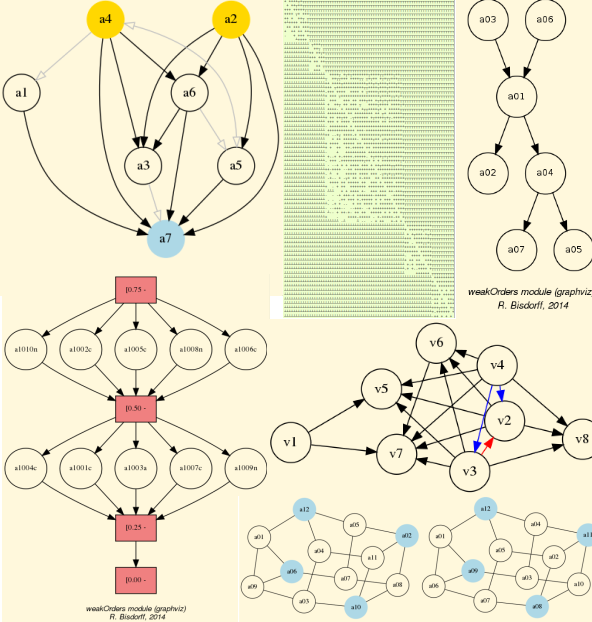
\includegraphics[scale=0.5]{introDoc3.png}
        \end{figure}

        \vspace{10mm}
        \textbf{\Huge {Tutorials and Advanced Topics}}

        \textbf{Raymond BISDORFF}

        \small Luxembourg,  2020

        \small  Last updated : \today
        
        \vspace{10mm}
        \begin{center}
        \emph{This documentation is dedicated to our}\\
        \emph{late colleague and dear friend}\\
         Prof. Marc ROUBENS.
        \end{center}

        %% \vfill adds at the bottom
        \vfill
        \textit{More documents are freely available }{\href{https://digraph3.readthedocs.io/en/latest}{here}}
    \end{titlepage}

    \clearpage
    \pagenumbering{arabic}

    
\pagestyle{plain}

    
    
\pagestyle{normal}
\phantomsection\label{\detokenize{pearls::doc}}
\begingroup
\sphinxsetup{%
      verbatimwithframe=false,
      VerbatimColor={named}{OldLace},
      %VerbatimHighlightColor={named}{Aqua},
      hintBorderColor={named}{LightCoral},
      attentionborder=3pt,
      attentionBorderColor={named}{Crimson},
      attentionBgColor={named}{FloralWhite},
      noteborder=2pt,
      noteBorderColor={named}{Olive},
      cautionborder=3pt,
      cautionBorderColor={named}{Cyan},
      cautionBgColor={named}{LightCyan}}


\phantomsection\label{\detokenize{pearls:pearls-label}}

\bigskip\hrule\bigskip


\textbf{\Large{B. Digraph3 Advanced Topics}}

\href{https://digraph3.readthedocs.io/en/latest/index.html}{HTML Version}
\vspace{5mm}

\sphinxAtStartPar
In this part of the \sphinxstylestrong{Digraph3} \sphinxstyleemphasis{documentation}, we provide an insight in computational enhancements one may get when working in a \sphinxstyleemphasis{bipolar\sphinxhyphen{}valued epistemic logic} framework, like \sphinxhyphen{} easily coping with \sphinxstyleemphasis{missing data} and uncertain criterion \sphinxstyleemphasis{significance weights}, \sphinxhyphen{} computing valued \sphinxstyleemphasis{ordinal correlations} between bipolar\sphinxhyphen{}valued outranking digraphs, \sphinxhyphen{} compting digraph kernels and solving bipolar\sphinxhyphen{}valued kernel equation systems and, \sphinxhyphen{} testing for stability and confidence of outranking statements when facing uncertain performance criteria significance weights or decision objectives’ importance weights.

\sphinxtableofcontents


\section{Enhancing the outranking based MCDA approach}
\label{\detokenize{pearls:enhancing-the-outranking-based-mcda-approach}}\label{\detokenize{pearls:enhancing-outranking-label}}\begin{quote}

\sphinxAtStartPar
“\sphinxstyleemphasis{The goal of our research was to design a resolution method} {[}..{]} \sphinxstyleemphasis{that is easy to put into practice, that requires as few and reliable hypotheses as possible, and that meets the needs} {[}of the decision maker{]}.”

\begin{flushright}
---Benayoun R, Roy B, Sussmann B %
\begin{footnote}[13]\sphinxAtStartFootnote
\sphinxcite{pearls:roy-1966p}
%
\end{footnote}
\end{flushright}
\end{quote}

\begin{sphinxShadowBox}
\begin{itemize}
\item {} 
\sphinxAtStartPar
\phantomsection\label{\detokenize{pearls:id84}}{\hyperref[\detokenize{pearls:on-confident-outrankings-with-uncertain-criteria-significance-weights}]{\sphinxcrossref{On confident outrankings with uncertain criteria significance weights}}} (\autopageref*{\detokenize{pearls:on-confident-outrankings-with-uncertain-criteria-significance-weights}})

\item {} 
\sphinxAtStartPar
\phantomsection\label{\detokenize{pearls:id85}}{\hyperref[\detokenize{pearls:on-stable-outrankings-with-ordinal-criteria-significance-weights}]{\sphinxcrossref{On stable outrankings with ordinal criteria significance weights}}} (\autopageref*{\detokenize{pearls:on-stable-outrankings-with-ordinal-criteria-significance-weights}})

\item {} 
\sphinxAtStartPar
\phantomsection\label{\detokenize{pearls:id86}}{\hyperref[\detokenize{pearls:on-unopposed-outrankings-with-multiple-decision-objectives}]{\sphinxcrossref{On unopposed outrankings with multiple decision objectives}}} (\autopageref*{\detokenize{pearls:on-unopposed-outrankings-with-multiple-decision-objectives}})

\end{itemize}
\end{sphinxShadowBox}


\subsection{On confident outrankings with uncertain criteria significance weights}
\label{\detokenize{pearls:on-confident-outrankings-with-uncertain-criteria-significance-weights}}\label{\detokenize{pearls:bipolar-valued-likelihood-tutorial-label}}
\begin{sphinxShadowBox}
\begin{itemize}
\item {} 
\sphinxAtStartPar
\phantomsection\label{\detokenize{pearls:id87}}{\hyperref[\detokenize{pearls:modelling-uncertain-criteria-significance-weights}]{\sphinxcrossref{Modelling uncertain criteria significance weights}}} (\autopageref*{\detokenize{pearls:modelling-uncertain-criteria-significance-weights}})

\item {} 
\sphinxAtStartPar
\phantomsection\label{\detokenize{pearls:id88}}{\hyperref[\detokenize{pearls:bipolar-valued-likelihood-of-at-least-as-good-as-situations}]{\sphinxcrossref{Bipolar\sphinxhyphen{}valued likelihood of ‘’at least as good as ” situations}}} (\autopageref*{\detokenize{pearls:bipolar-valued-likelihood-of-at-least-as-good-as-situations}})

\item {} 
\sphinxAtStartPar
\phantomsection\label{\detokenize{pearls:id89}}{\hyperref[\detokenize{pearls:confidence-level-of-outranking-situations}]{\sphinxcrossref{Confidence level of outranking situations}}} (\autopageref*{\detokenize{pearls:confidence-level-of-outranking-situations}})

\end{itemize}
\end{sphinxShadowBox}

\sphinxAtStartPar
When modelling preferences following the outranking approach, the signs of the majority margins do sharply distribute validation and invalidation of pairwise outranking situations. How can we be confident in the resulting outranking digraph, when we acknowledge the usual imprecise knowledge of criteria significance weights coupled with small majority margins?

\sphinxAtStartPar
To answer this question, one usually requires \sphinxstyleemphasis{qualified} majority margins for confirming outranking situations. But how to choose such a qualifying majority level: two third, three fourth of the significance weights ?

\sphinxAtStartPar
In this tutorial we propose to link the qualifying significance majority with a required alpha\%\sphinxhyphen{}confidence level. We model therefore the significance weights as random variables following more or less widespread distributions around an average significance value that corresponds to the given deterministic weight. As the bipolar\sphinxhyphen{}valued random credibility of an outranking statement hence results from the simple sum of positive or negative independent random variables, we may apply the Central Limit Theorem (CLT) for computing the \sphinxstyleemphasis{bipolar likelihood} that the expected majority margin will indeed be positive, respectively negative.


\subsubsection{Modelling uncertain criteria significance weights}
\label{\detokenize{pearls:modelling-uncertain-criteria-significance-weights}}
\sphinxAtStartPar
Let us consider the significance weights of a family \sphinxstyleemphasis{F} of \sphinxstyleemphasis{m} criteria to be \sphinxstylestrong{independent random variables} \sphinxstyleemphasis{Wj}, distributing the potential significance weights of each criterion \sphinxstyleemphasis{j} = 1, …, \sphinxstyleemphasis{m} around a mean value \sphinxstyleemphasis{E(Wj)} with variance \sphinxstyleemphasis{V(Wj)}.

\sphinxAtStartPar
Choosing a specific stochastic model of uncertainty is usually application specific. In the limited scope of this tutorial, we will illustrate the consequence of this design decision on the resulting outranking modelling with four slightly different models for taking into account the uncertainty with which we know the numerical significance weights: \sphinxstyleemphasis{uniform}, \sphinxstyleemphasis{triangular}, and two models of \sphinxstyleemphasis{Beta laws}, one more \sphinxstyleemphasis{widespread} and, the other, more \sphinxstyleemphasis{concentrated}.

\sphinxAtStartPar
When considering, for instance, that the potential range of a significance weight is distributed between 0 and two times its mean value, we obtain the following random variates:
\begin{enumerate}
\sphinxsetlistlabels{\arabic}{enumi}{enumii}{}{.}%
\item {} 
\sphinxAtStartPar
A continuous \sphinxstylestrong{uniform} distribution on the range 0 to \sphinxstyleemphasis{2E(Wj)}. Thus \sphinxstyleemphasis{Wj} \textasciitilde{} U(0, \sphinxstyleemphasis{2E(Wj)}) and \sphinxstyleemphasis{V(Wj)} = 1/3(\sphinxstyleemphasis{E(Wj)})\textasciicircum{}2;

\item {} 
\sphinxAtStartPar
A \sphinxstylestrong{symmetric beta} distribution with, for instance,
parameters  \sphinxstyleemphasis{alpha} = 2 and \sphinxstyleemphasis{beta} = 2. Thus, \sphinxstyleemphasis{Wi} \textasciitilde{}
Beta(2,2) * \sphinxstyleemphasis{2E(Wj)} and \sphinxstyleemphasis{V(Wj)} = 1/5(\sphinxstyleemphasis{E(Wj)})\textasciicircum{}2.

\item {} 
\sphinxAtStartPar
A \sphinxstylestrong{symmetric triangular} distribution on the same range with
mode \sphinxstyleemphasis{E(Wj)}. Thus \sphinxstyleemphasis{Wj} \textasciitilde{} Tr(0, \sphinxstyleemphasis{2E(Wj)}, \sphinxstyleemphasis{E(Wj)}) with
\sphinxstyleemphasis{V(Wj)} = 1/6(\sphinxstyleemphasis{E(Wj)})\textasciicircum{}2;

\item {} 
\sphinxAtStartPar
A \sphinxstylestrong{narrower beta} distribution with for instance
parameters \sphinxstyleemphasis{alpha} = 4 and \sphinxstyleemphasis{beta} = 4. Thus \sphinxstyleemphasis{Wj} \textasciitilde{} Beta(4,4) *
\sphinxstyleemphasis{2E(Wj)} , \sphinxstyleemphasis{V(Wj)} = 1/9(\sphinxstyleemphasis{E(Wj)})\textasciicircum{}2.

\end{enumerate}

\begin{figure}[H]
\centering
\capstart

\noindent\sphinxincludegraphics[width=450\sphinxpxdimen]{{weightDistributions}.png}
\caption{Four models of uncertain significance weights}\label{\detokenize{pearls:weightdistributions}}\end{figure}

\sphinxAtStartPar
It is worthwhile noticing that these four uncertainty models all admit the same expected value, \sphinxstyleemphasis{E(Wj)}, however, with a respective variance which goes decreasing from 1/3, to 1/9 of the square of \sphinxstyleemphasis{E(W)} (see \hyperref[\detokenize{pearls:weightdistributions}]{Fig.\@ \ref{\detokenize{pearls:weightdistributions}}}).


\subsubsection{Bipolar\sphinxhyphen{}valued likelihood of ‘’at least as good as ” situations}
\label{\detokenize{pearls:bipolar-valued-likelihood-of-at-least-as-good-as-situations}}
\sphinxAtStartPar
Let \sphinxstyleemphasis{A} = \{\sphinxstyleemphasis{x}, \sphinxstyleemphasis{y}, \sphinxstyleemphasis{z},…\} be a finite set of \sphinxstyleemphasis{n} potential decision actions, evaluated on \sphinxstyleemphasis{F} = \{1,…, \sphinxstyleemphasis{m}\}, a \sphinxstyleemphasis{finite} and \sphinxstyleemphasis{coherent} family of \sphinxstyleemphasis{m} performance criteria. On each criterion \sphinxstyleemphasis{j} in \sphinxstyleemphasis{F}, the decision actions are evaluated on a real performance scale {[}0; \sphinxstyleemphasis{Mj} {]}, supporting an upper\sphinxhyphen{}closed indifference threshold \sphinxstyleemphasis{indj} and a lower\sphinxhyphen{}closed preference threshold \sphinxstyleemphasis{prj} such that 0 \textless{}= \sphinxstyleemphasis{indj} \textless{} \sphinxstyleemphasis{prj} \textless{}= \sphinxstyleemphasis{Mj}. The marginal performance of object \sphinxstyleemphasis{x} on criterion \sphinxstyleemphasis{j} is denoted \sphinxstyleemphasis{xj}. Each criterion \sphinxstyleemphasis{j} is thus characterising a marginal double threshold order \(\geq_j\) on \sphinxstyleemphasis{A} (see \hyperref[\detokenize{pearls:rcharacteristic}]{Fig.\@ \ref{\detokenize{pearls:rcharacteristic}}}):
\begin{quote}
\begin{equation*}
\begin{split}r(x \geq_j y) \; = \; \begin{cases} +1 \quad \text{if} \quad x_j - y_j \geq -ind_j,\\  -1 \quad \text{if} \quad x_j - y_j \leq -pr_j,\\ 0 \quad \text{otherwise}. \end{cases}\end{split}
\end{equation*}\end{quote}
\begin{description}
\sphinxlineitem{Semantics of the marginal bipolar\sphinxhyphen{}valued characteristic function:}\begin{itemize}
\item {} 
\sphinxAtStartPar
+1 signifies \sphinxstyleemphasis{x} is performing at least as good as \sphinxstyleemphasis{y} on
criterion \sphinxstyleemphasis{j},

\item {} 
\sphinxAtStartPar
\sphinxhyphen{}1 signifies that \sphinxstyleemphasis{x} is not performing at least as good as \sphinxstyleemphasis{y} on
criterion \sphinxstyleemphasis{j},

\item {} 
\sphinxAtStartPar
0 signifies that it is
unclear whether, on criterion \sphinxstyleemphasis{j}, \sphinxstyleemphasis{x} is performing at least as good as \sphinxstyleemphasis{y}.

\end{itemize}

\end{description}

\begin{figure}[H]
\centering
\capstart

\noindent\sphinxincludegraphics[width=450\sphinxpxdimen]{{rCharacteristic}.png}
\caption{Bipolar\sphinxhyphen{}valued outranking characteristic function}\label{\detokenize{pearls:rcharacteristic}}\end{figure}

\sphinxAtStartPar
Each criterion \sphinxstyleemphasis{j} in \sphinxstyleemphasis{F} contributes the random significance \sphinxstyleemphasis{Wj} of his ‘\sphinxstyleemphasis{at least as good as}’ characteristic \(r(x \geq_j y)\) to the global characteristic \(\tilde{r}(x \geq y)\) in the following way:
\begin{quote}
\begin{equation*}
\begin{split}\tilde{r}(x \geq y) \; = \; \sum_{j \in F} W_j \times r(x \geq_j y) )\end{split}
\end{equation*}\end{quote}

\sphinxAtStartPar
Thus, \(\tilde{r}(x \geq y)\) becomes a simple sum of positive or negative independent random variables with known means and variances where \(\tilde{r}(x \geq y) \, > \, 0\) signifies \sphinxstyleemphasis{x} is globally performing at least as good as \sphinxstyleemphasis{y}, \(\tilde{r}(x \geq y) \, < \, 0\) signifies that \sphinxstyleemphasis{x} is not globally performing at least as good as \sphinxstyleemphasis{y}, and \(\tilde{r}(x \geq y)\,=\,0\) signifies that it is unclear whether \sphinxstyleemphasis{x} is globally performing at least as good as \sphinxstyleemphasis{y}.

\sphinxAtStartPar
From the \sphinxstyleemphasis{Central Limit Theorem} (CLT), we know that such a sum of random variables leads, with \sphinxstyleemphasis{m} getting large, to a Gaussian distribution \sphinxstyleemphasis{Y} with
\begin{quote}

\sphinxAtStartPar
\(E(Y ) = \sum_{j \in F} \big(\,E(W_j) \times r(x \geq_j y)\,\big)\), and

\sphinxAtStartPar
\(V(Y) = \sum_{j \in F} \big(\,V(W_j)\times |r(x \geq_j y)|\,\big)\).
\end{quote}

\sphinxAtStartPar
And the \sphinxstylestrong{likelihood of validation}, respectively \sphinxstylestrong{invalidation} of an ‘\sphinxstyleemphasis{at least as good as}’ situation, denoted \(lh(x \geq y)\),  may hence be assessed by the probability \sphinxstyleemphasis{P(Y\textgreater{}0)} = 1.0 \sphinxhyphen{} \sphinxstyleemphasis{P(Y\textless{}=0)} that \sphinxstyleemphasis{Y} takes a positive, resp. \sphinxstyleemphasis{P(Y\textless{}0)} takes a negative value. In the bipolar\sphinxhyphen{}valued case here, we can judiciously make usage of the standard Gaussian \sphinxstylestrong{error function} , i.e. the bipolar \sphinxstyleemphasis{2P(Z)} \sphinxhyphen{} 1.0 version of the standard Gaussian \sphinxstyleemphasis{P(Z)} probability distribution function:
\begin{quote}
\begin{equation*}
\begin{split}lh(x \geq y) \;=\; -\text{erf}\big(\frac{1}{\sqrt{2}}\frac{-E(Y)}{\sqrt{V(Y)}} \big)\end{split}
\end{equation*}\end{quote}

\sphinxAtStartPar
The range of the bipolar\sphinxhyphen{}valued \(lh(x \geq y)\) hence becomes {[}\sphinxhyphen{}1.0;+1.0{]}, and \(-lh(x \geq y) \,=\, lh(x \not\geq y)\) , i.e. a \sphinxstylestrong{negative likelihood} represents the likelihood of the correspondent \sphinxstylestrong{negated} ‘\sphinxstyleemphasis{at least as good as}’ situation. A likelihood of +1.0 (resp. \sphinxhyphen{}1.0) means the corresponding preferential situation appears \sphinxstylestrong{certainly validated} (resp. \sphinxstylestrong{invalidated}).

\sphinxAtStartPar
\sphinxstylestrong{Example}

\sphinxAtStartPar
Let \sphinxstyleemphasis{x} and \sphinxstyleemphasis{y} be evaluated wrt 7 equisignificant criteria; Four criteria positively support that \sphinxstyleemphasis{x} is \sphinxstyleemphasis{as least as good performing} than \sphinxstyleemphasis{y} and three criteria support that \sphinxstyleemphasis{x} is \sphinxstyleemphasis{not at least as good} performing than \sphinxstyleemphasis{y}. Suppose \sphinxstyleemphasis{E(Wj)} = \sphinxstyleemphasis{w} for \sphinxstyleemphasis{j} = 1,…,7 and \sphinxstyleemphasis{Wj} \textasciitilde{} Tr(0, \sphinxstyleemphasis{2w}, \sphinxstyleemphasis{w}) for \sphinxstyleemphasis{j} = 1,…7. The expected value of the global ‘\sphinxstyleemphasis{at least as good as}’ characteristic value becomes: \(E\big(\tilde{r}(x \geq y)\big)\, = \, 4w - 3w = w\) with a variance \(V\big(\tilde{r}(x \geq y)\big)\,=\, 7\frac{1}{6}w^2\).

\sphinxAtStartPar
If \sphinxstyleemphasis{w} = 1, \(E\big(\tilde{r}(x \geq y)\big)\, = \, 1\) and \(sd\big(\tilde{r}(x \geq y)\big)\,=\, 1.08\). By the CLT, the bipolar likelihood of the \sphinxstyleemphasis{at least as good} performing situation becomes: \(lh(x \geq y)\,=\, 0.66\), which corresponds to a global support of (0.66 + 1.0)/2 = 83\% of the criteria significance weights.

\sphinxAtStartPar
A \sphinxstyleemphasis{Monte Carlo} simulation with 10 000 runs empirically confirms the effective convergence to a Gaussian (see \hyperref[\detokenize{pearls:simullikelihood}]{Fig.\@ \ref{\detokenize{pearls:simullikelihood}}} realised with \sphinxstyleemphasis{gretl} %
\begin{footnote}[4]\sphinxAtStartFootnote
The \sphinxstyleemphasis{Gnu Regression, Econometrics and Time\sphinxhyphen{}series Library} \sphinxurl{http://gretl.sourceforge.net/}
%
\end{footnote} ).

\begin{figure}[H]
\centering
\capstart

\noindent\sphinxincludegraphics[width=550\sphinxpxdimen]{{simulLikelihood}.png}
\caption{Distribution of 10 000 random outranking characteristic values}\label{\detokenize{pearls:simullikelihood}}\end{figure}

\sphinxAtStartPar
Indeed, \(\tilde{r}(x \geq y) \leadsto Y = \mathcal{N}(1.03,1.089)\), with an empirical probability of observing a negative majority margin of about 17\%.


\subsubsection{Confidence level of outranking situations}
\label{\detokenize{pearls:confidence-level-of-outranking-situations}}
\sphinxAtStartPar
Now, following the classical outranking approach (see \sphinxcite{pearls:bis-2013p} ), we may say, from an epistemic perspective, that decision action \sphinxstyleemphasis{x} \sphinxstylestrong{outranks} decision action \sphinxstyleemphasis{y} at \sphinxstyleemphasis{confidence} level \sphinxstyleemphasis{alpha} \%, when
\begin{enumerate}
\sphinxsetlistlabels{\arabic}{enumi}{enumii}{}{.}%
\item {} 
\sphinxAtStartPar
an expected majority of criteria validates, at confidence level \sphinxstyleemphasis{alpha} \% or higher, a global ‘\sphinxstyleemphasis{at least as good as}’ situation between \sphinxstyleemphasis{x} and \sphinxstyleemphasis{y}, and

\item {} 
\sphinxAtStartPar
no considerably less performing is observed on a discordant criterion.

\end{enumerate}

\sphinxAtStartPar
Dually, decision action \sphinxstyleemphasis{x} \sphinxstylestrong{does not outrank} decision action \sphinxstyleemphasis{y} at
confidence level \sphinxstyleemphasis{alpha} \%, when
\begin{enumerate}
\sphinxsetlistlabels{\arabic}{enumi}{enumii}{}{.}%
\item {} 
\sphinxAtStartPar
an expected majority of criteria at confidence level \sphinxstyleemphasis{alpha} \% or higher, invalidates a global ‘\sphinxstyleemphasis{at least as good as}’ situation between \sphinxstyleemphasis{x} and \sphinxstyleemphasis{y}, and

\item {} 
\sphinxAtStartPar
no considerably better performing situation is observed on a concordant criterion.

\end{enumerate}

\sphinxAtStartPar
\sphinxstylestrong{Time for a coded example}

\sphinxAtStartPar
Let us consider the following random performance tableau.

\begin{sphinxVerbatim}[commandchars=\\\{\},numbers=left,firstnumber=1,stepnumber=1]
\PYG{g+gp}{\PYGZgt{}\PYGZgt{}\PYGZgt{} }\PYG{k+kn}{from} \PYG{n+nn}{randomPerfTabs} \PYG{k+kn}{import} \PYG{n}{RandomPerformanceTableau}
\PYG{g+gp}{\PYGZgt{}\PYGZgt{}\PYGZgt{} }\PYG{n}{t} \PYG{o}{=} \PYG{n}{RandomPerformanceTableau}\PYG{p}{(}
\PYG{g+gp}{... }         \PYG{n}{numberOfActions}\PYG{o}{=}\PYG{l+m+mi}{7}\PYG{p}{,}
\PYG{g+gp}{... }         \PYG{n}{numberOfCriteria}\PYG{o}{=}\PYG{l+m+mi}{7}\PYG{p}{,}\PYG{n}{seed}\PYG{o}{=}\PYG{l+m+mi}{100}\PYG{p}{)}

\PYG{g+gp}{\PYGZgt{}\PYGZgt{}\PYGZgt{} }\PYG{n}{t}\PYG{o}{.}\PYG{n}{showPerformanceTableau}\PYG{p}{(}\PYG{n}{Transposed}\PYG{o}{=}\PYG{k+kc}{True}\PYG{p}{)}
\PYG{g+go}{ *\PYGZhy{}\PYGZhy{}\PYGZhy{}\PYGZhy{}  performance tableau \PYGZhy{}\PYGZhy{}\PYGZhy{}\PYGZhy{}\PYGZhy{}*}
\PYG{g+go}{ criteria | weights |   \PYGZsq{}a1\PYGZsq{}   \PYGZsq{}a2\PYGZsq{}   \PYGZsq{}a3\PYGZsq{}   \PYGZsq{}a4\PYGZsq{}   \PYGZsq{}a5\PYGZsq{}   \PYGZsq{}a6\PYGZsq{}   \PYGZsq{}a7\PYGZsq{}}
\PYG{g+go}{ \PYGZhy{}\PYGZhy{}\PYGZhy{}\PYGZhy{}\PYGZhy{}\PYGZhy{}\PYGZhy{}\PYGZhy{}\PYGZhy{}|\PYGZhy{}\PYGZhy{}\PYGZhy{}\PYGZhy{}\PYGZhy{}\PYGZhy{}\PYGZhy{}\PYGZhy{}\PYGZhy{}\PYGZhy{}\PYGZhy{}\PYGZhy{}\PYGZhy{}\PYGZhy{}\PYGZhy{}\PYGZhy{}\PYGZhy{}\PYGZhy{}\PYGZhy{}\PYGZhy{}\PYGZhy{}\PYGZhy{}\PYGZhy{}\PYGZhy{}\PYGZhy{}\PYGZhy{}\PYGZhy{}\PYGZhy{}\PYGZhy{}\PYGZhy{}\PYGZhy{}\PYGZhy{}\PYGZhy{}\PYGZhy{}\PYGZhy{}\PYGZhy{}\PYGZhy{}\PYGZhy{}\PYGZhy{}\PYGZhy{}\PYGZhy{}\PYGZhy{}\PYGZhy{}\PYGZhy{}\PYGZhy{}\PYGZhy{}\PYGZhy{}\PYGZhy{}\PYGZhy{}\PYGZhy{}\PYGZhy{}\PYGZhy{}\PYGZhy{}\PYGZhy{}\PYGZhy{}\PYGZhy{}\PYGZhy{}\PYGZhy{}\PYGZhy{}\PYGZhy{}}
\PYG{g+go}{    \PYGZsq{}g1\PYGZsq{}  |     1   |  15.17  44.51  57.87  58.00  24.22  29.10  96.58}
\PYG{g+go}{    \PYGZsq{}g2\PYGZsq{}  |     1   |  82.29  43.90    NA   35.84  29.12  34.79  62.22}
\PYG{g+go}{    \PYGZsq{}g3\PYGZsq{}  |     1   |  44.23  19.10  27.73  41.46  22.41  21.52  56.90}
\PYG{g+go}{    \PYGZsq{}g4\PYGZsq{}  |     1   |  46.37  16.22  21.53  51.16  77.01  39.35  32.06}
\PYG{g+go}{    \PYGZsq{}g5\PYGZsq{}  |     1   |  47.67  14.81  79.70  67.48    NA   90.72  80.16}
\PYG{g+go}{    \PYGZsq{}g6\PYGZsq{}  |     1   |  69.62  45.49  22.03  33.83  31.83    NA   48.80}
\PYG{g+go}{    \PYGZsq{}g7\PYGZsq{}  |     1   |  82.88  41.66  12.82  21.92  75.74  15.45   6.05}
\end{sphinxVerbatim}

\sphinxAtStartPar
For the corresponding confident outranking digraph, we require a confidence level of \sphinxstyleemphasis{alpha} = 90\%. The \sphinxcode{\sphinxupquote{ConfidentBipolarOutrankingDigraph}} class provides such a construction.

\fvset{hllines={, 4,}}%
\begin{sphinxVerbatim}[commandchars=\\\{\},numbers=left,firstnumber=1,stepnumber=1]
\PYG{g+gp}{\PYGZgt{}\PYGZgt{}\PYGZgt{} }\PYG{k+kn}{from} \PYG{n+nn}{outrankingDigraphs} \PYG{k+kn}{import}\PYGZbs{}
\PYG{g+gp}{... }                      \PYG{n}{ConfidentBipolarOutrankingDigraph}

\PYG{g+gp}{\PYGZgt{}\PYGZgt{}\PYGZgt{} }\PYG{n}{g90} \PYG{o}{=} \PYG{n}{ConfidentBipolarOutrankingDigraph}\PYG{p}{(}\PYG{n}{t}\PYG{p}{,}\PYG{n}{confidence}\PYG{o}{=}\PYG{l+m+mi}{90}\PYG{p}{)}
\PYG{g+gp}{\PYGZgt{}\PYGZgt{}\PYGZgt{} }\PYG{n+nb}{print}\PYG{p}{(}\PYG{n}{g90}\PYG{p}{)}
\PYG{g+go}{ *\PYGZhy{}\PYGZhy{}\PYGZhy{}\PYGZhy{}\PYGZhy{}\PYGZhy{}\PYGZhy{} Object instance description \PYGZhy{}\PYGZhy{}\PYGZhy{}\PYGZhy{}\PYGZhy{}\PYGZhy{}*}
\PYG{g+go}{ Instance class      : ConfidentBipolarOutrankingDigraph}
\PYG{g+go}{ Instance name       : rel\PYGZus{}randomperftab\PYGZus{}CLT}
\PYG{g+go}{ \PYGZsh{} Actions           : 7}
\PYG{g+go}{ \PYGZsh{} Criteria          : 7}
\PYG{g+go}{ Size                : 15}
\PYG{g+go}{ Uncertainty model   : triangular(a=0,b=2w)}
\PYG{g+go}{ Likelihood domain   : [\PYGZhy{}1.0;+1.0]}
\PYG{g+go}{ Confidence level    : 0.80 (90.0\PYGZpc{})}
\PYG{g+go}{ Confident majority  : 0.14 (57.1\PYGZpc{})}
\PYG{g+go}{ Determinateness (\PYGZpc{}) : 62.07}
\PYG{g+go}{ Valuation domain    : [\PYGZhy{}1.00;1.00]}
\PYG{g+go}{ Attributes          : [\PYGZsq{}name\PYGZsq{}, \PYGZsq{}bipolarConfidenceLevel\PYGZsq{},}
\PYG{g+go}{                        \PYGZsq{}distribution\PYGZsq{}, \PYGZsq{}betaParameter\PYGZsq{}, \PYGZsq{}actions\PYGZsq{},}
\PYG{g+go}{                        \PYGZsq{}order\PYGZsq{}, \PYGZsq{}valuationdomain\PYGZsq{}, \PYGZsq{}criteria\PYGZsq{},}
\PYG{g+go}{                        \PYGZsq{}evaluation\PYGZsq{}, \PYGZsq{}concordanceRelation\PYGZsq{},}
\PYG{g+go}{                        \PYGZsq{}vetos\PYGZsq{}, \PYGZsq{}negativeVetos\PYGZsq{},}
\PYG{g+go}{                        \PYGZsq{}largePerformanceDifferencesCount\PYGZsq{},}
\PYG{g+go}{                        \PYGZsq{}likelihoods\PYGZsq{}, \PYGZsq{}confidenceCutLevel\PYGZsq{},}
\PYG{g+go}{                        \PYGZsq{}relation\PYGZsq{}, \PYGZsq{}gamma\PYGZsq{}, \PYGZsq{}notGamma\PYGZsq{}]}
\end{sphinxVerbatim}
\sphinxresetverbatimhllines

\sphinxAtStartPar
The resulting 90\% confident expected outranking relation is shown below.

\fvset{hllines={, 22, 23,}}%
\begin{sphinxVerbatim}[commandchars=\\\{\},numbers=left,firstnumber=1,stepnumber=1]
\PYG{g+gp}{\PYGZgt{}\PYGZgt{}\PYGZgt{} }\PYG{n}{g90}\PYG{o}{.}\PYG{n}{showRelationTable}\PYG{p}{(}\PYG{n}{LikelihoodDenotation}\PYG{o}{=}\PYG{k+kc}{True}\PYG{p}{)}
\PYG{g+go}{ * \PYGZhy{}\PYGZhy{}\PYGZhy{}\PYGZhy{} Outranking Relation Table \PYGZhy{}\PYGZhy{}\PYGZhy{}\PYGZhy{}\PYGZhy{}}
\PYG{g+go}{ r/(lh) |  \PYGZsq{}a1\PYGZsq{}       \PYGZsq{}a2\PYGZsq{}    \PYGZsq{}a3\PYGZsq{}    \PYGZsq{}a4\PYGZsq{}    \PYGZsq{}a5\PYGZsq{}    \PYGZsq{}a6\PYGZsq{}    \PYGZsq{}a7\PYGZsq{}}
\PYG{g+go}{ \PYGZhy{}\PYGZhy{}\PYGZhy{}\PYGZhy{}\PYGZhy{}\PYGZhy{}\PYGZhy{}|\PYGZhy{}\PYGZhy{}\PYGZhy{}\PYGZhy{}\PYGZhy{}\PYGZhy{}\PYGZhy{}\PYGZhy{}\PYGZhy{}\PYGZhy{}\PYGZhy{}\PYGZhy{}\PYGZhy{}\PYGZhy{}\PYGZhy{}\PYGZhy{}\PYGZhy{}\PYGZhy{}\PYGZhy{}\PYGZhy{}\PYGZhy{}\PYGZhy{}\PYGZhy{}\PYGZhy{}\PYGZhy{}\PYGZhy{}\PYGZhy{}\PYGZhy{}\PYGZhy{}\PYGZhy{}\PYGZhy{}\PYGZhy{}\PYGZhy{}\PYGZhy{}\PYGZhy{}\PYGZhy{}\PYGZhy{}\PYGZhy{}\PYGZhy{}\PYGZhy{}\PYGZhy{}\PYGZhy{}\PYGZhy{}\PYGZhy{}\PYGZhy{}\PYGZhy{}\PYGZhy{}\PYGZhy{}\PYGZhy{}\PYGZhy{}\PYGZhy{}\PYGZhy{}\PYGZhy{}\PYGZhy{}\PYGZhy{}\PYGZhy{}\PYGZhy{}\PYGZhy{}\PYGZhy{}\PYGZhy{}}
\PYG{g+go}{   \PYGZsq{}a1\PYGZsq{} | +0.00   +0.71   +0.29   +0.29   +0.29   +0.29   +0.00}
\PYG{g+go}{        | ( \PYGZhy{} )  (+1.00) (+0.95) (+0.95) (+0.95) (+0.95) (+0.65)}
\PYG{g+go}{   \PYGZsq{}a2\PYGZsq{} | \PYGZhy{}0.71   +0.00   \PYGZhy{}0.29   +0.00   +0.00   +0.29   \PYGZhy{}0.57}
\PYG{g+go}{        |(\PYGZhy{}1.00)  ( \PYGZhy{} )  (\PYGZhy{}0.95) (\PYGZhy{}0.65) (+0.73) (+0.95) (\PYGZhy{}1.00)}
\PYG{g+go}{   \PYGZsq{}a3\PYGZsq{} | \PYGZhy{}0.29   +0.29   +0.00   \PYGZhy{}0.29   +0.00   +0.00   \PYGZhy{}0.29}
\PYG{g+go}{        |(\PYGZhy{}0.95) (+0.95)  ( \PYGZhy{} )  (\PYGZhy{}0.95) (\PYGZhy{}0.73) (\PYGZhy{}0.00) (\PYGZhy{}0.95)}
\PYG{g+go}{   \PYGZsq{}a4\PYGZsq{} | +0.00   +0.00   +0.57   +0.00   +0.29   +0.57   \PYGZhy{}0.43}
\PYG{g+go}{        |(\PYGZhy{}0.00) (+0.65) (+1.00)  ( \PYGZhy{} )  (+0.95) (+1.00) (\PYGZhy{}0.99)}
\PYG{g+go}{   \PYGZsq{}a5\PYGZsq{} | \PYGZhy{}0.29   +0.00   +0.00   +0.00   +0.00   +0.29   \PYGZhy{}0.29}
\PYG{g+go}{        |(\PYGZhy{}0.95) (\PYGZhy{}0.00) (+0.73) (\PYGZhy{}0.00)  ( \PYGZhy{} )  (+0.99) (\PYGZhy{}0.95)}
\PYG{g+go}{   \PYGZsq{}a6\PYGZsq{} | \PYGZhy{}0.29   +0.00   +0.00   \PYGZhy{}0.29   +0.00   +0.00   +0.00}
\PYG{g+go}{        |(\PYGZhy{}0.95) (\PYGZhy{}0.00) (+0.73) (\PYGZhy{}0.95) (+0.73)  ( \PYGZhy{} )  (\PYGZhy{}0.00)}
\PYG{g+go}{   \PYGZsq{}a7\PYGZsq{} | +0.00   +0.71   +0.57   +0.43   +0.29   +0.00   +0.00}
\PYG{g+go}{        |(\PYGZhy{}0.65) (+1.00) (+1.00) (+0.99) (+0.95) (\PYGZhy{}0.00)  ( \PYGZhy{} )}
\PYG{g+go}{ Valuation domain   : [\PYGZhy{}1.000; +1.000]}
\PYG{g+go}{ Uncertainty model  : triangular(a=2.0,b=2.0)}
\PYG{g+go}{ Likelihood domain  : [\PYGZhy{}1.0;+1.0]}
\PYG{g+go}{ Confidence level   : 0.80 (90.0\PYGZpc{})}
\PYG{g+go}{ Confident majority : 0.14 (57.1\PYGZpc{})}
\PYG{g+go}{ Determinateness    : 0.24 (62.1\PYGZpc{})}
\end{sphinxVerbatim}
\sphinxresetverbatimhllines

\sphinxAtStartPar
The (\sphinxstyleemphasis{lh}) figures, indicated in the table above, correspond to bipolar likelihoods and the required bipolar confidence level equals (0.90+1.0)/2 = 0.80 (see Line 22 above). Action ‘\sphinxstyleemphasis{a1}’ thus confidently outranks all other actions, except ‘\sphinxstyleemphasis{a7}’ where the actual likelihood (+0.65) is lower than the required one (0.80) and we furthermore observe a considerable counter\sphinxhyphen{}performance on criterion ‘\sphinxstyleemphasis{g1}’.

\sphinxAtStartPar
Notice also the lack of confidence in the outranking situations we observe between action ‘\sphinxstyleemphasis{a2}’ and actions ‘\sphinxstyleemphasis{a4}’ and ‘\sphinxstyleemphasis{a5}’. In the deterministic case we would have \(r(a2 \geq a4) \,=\, -0.143\) and \(r(a2 \geq a5) \,=\, +0.143\) . All outranking situations with a characteristic value lower or equal to abs(0.143), i.e. a majority support of 1.143/2 = 57.1\% and less, appear indeed to be \sphinxstyleemphasis{not confident} at level 90\% (see Line 23 above).

\sphinxAtStartPar
We may draw the corresponding strict 90\%\sphinxhyphen{}confident outranking digraph, oriented by its initial and terminal \sphinxstyleemphasis{strict} prekernels (see \hyperref[\detokenize{pearls:confidentoutranking}]{Fig.\@ \ref{\detokenize{pearls:confidentoutranking}}}).

\fvset{hllines={, 1, 2,}}%
\begin{sphinxVerbatim}[commandchars=\\\{\},numbers=left,firstnumber=1,stepnumber=1]
\PYG{g+gp}{\PYGZgt{}\PYGZgt{}\PYGZgt{} }\PYG{n}{gcd90} \PYG{o}{=} \PYG{o}{\PYGZti{}} \PYG{p}{(}\PYG{o}{\PYGZhy{}}\PYG{n}{g90}\PYG{p}{)}
\PYG{g+gp}{\PYGZgt{}\PYGZgt{}\PYGZgt{} }\PYG{n}{gcd90}\PYG{o}{.}\PYG{n}{showPreKernels}\PYG{p}{(}\PYG{p}{)}
\PYG{g+go}{ *\PYGZhy{}\PYGZhy{}\PYGZhy{} Computing preKernels \PYGZhy{}\PYGZhy{}\PYGZhy{}*}
\PYG{g+go}{ Dominant preKernels :}
\PYG{g+go}{ [\PYGZsq{}a1\PYGZsq{}, \PYGZsq{}a7\PYGZsq{}]}
\PYG{g+go}{    independence :  0.0}
\PYG{g+go}{    dominance    :  0.2857}
\PYG{g+go}{    absorbency   :  \PYGZhy{}0.7143}
\PYG{g+go}{    covering     :  0.800}
\PYG{g+go}{ Absorbent preKernels :}
\PYG{g+go}{ [\PYGZsq{}a2\PYGZsq{}, \PYGZsq{}a5\PYGZsq{}, \PYGZsq{}a6\PYGZsq{}]}
\PYG{g+go}{    independence :  0.0}
\PYG{g+go}{    dominance    :  \PYGZhy{}0.2857}
\PYG{g+go}{    absorbency   :  0.2857}
\PYG{g+go}{    covered      :  0.583}
\PYG{g+gp}{\PYGZgt{}\PYGZgt{}\PYGZgt{} }\PYG{n}{gcd90}\PYG{o}{.}\PYG{n}{exportGraphViz}\PYG{p}{(}\PYG{n}{fileName}\PYG{o}{=}\PYG{l+s+s1}{\PYGZsq{}}\PYG{l+s+s1}{confidentOutranking}\PYG{l+s+s1}{\PYGZsq{}}\PYG{p}{,}
\PYG{g+gp}{... }    \PYG{n}{firstChoice}\PYG{o}{=}\PYG{p}{[}\PYG{l+s+s1}{\PYGZsq{}}\PYG{l+s+s1}{a1}\PYG{l+s+s1}{\PYGZsq{}}\PYG{p}{,} \PYG{l+s+s1}{\PYGZsq{}}\PYG{l+s+s1}{a7}\PYG{l+s+s1}{\PYGZsq{}}\PYG{p}{]}\PYG{p}{,}\PYG{n}{lastChoice}\PYG{o}{=}\PYG{p}{[}\PYG{l+s+s1}{\PYGZsq{}}\PYG{l+s+s1}{a2}\PYG{l+s+s1}{\PYGZsq{}}\PYG{p}{,} \PYG{l+s+s1}{\PYGZsq{}}\PYG{l+s+s1}{a5}\PYG{l+s+s1}{\PYGZsq{}}\PYG{p}{,} \PYG{l+s+s1}{\PYGZsq{}}\PYG{l+s+s1}{a6}\PYG{l+s+s1}{\PYGZsq{}}\PYG{p}{]}\PYG{p}{)}

\PYG{g+go}{ *\PYGZhy{}\PYGZhy{}\PYGZhy{}\PYGZhy{} exporting a dot file for GraphViz tools \PYGZhy{}\PYGZhy{}\PYGZhy{}\PYGZhy{}\PYGZhy{}\PYGZhy{}\PYGZhy{}\PYGZhy{}\PYGZhy{}*}
\PYG{g+go}{ Exporting to confidentOutranking.dot}
\PYG{g+go}{ dot \PYGZhy{}Grankdir=BT \PYGZhy{}Tpng confidentOutranking.dot \PYGZhy{}o confidentOutranking.png}
\end{sphinxVerbatim}
\sphinxresetverbatimhllines

\begin{figure}[H]
\centering
\capstart

\noindent\sphinxincludegraphics[width=350\sphinxpxdimen]{{confidentOutranking}.png}
\caption{Strict 90\%\sphinxhyphen{}confident outranking digraph oriented by its prekernels}\label{\detokenize{pearls:confidentoutranking}}\end{figure}

\sphinxAtStartPar
Now, what becomes this 90\%\sphinxhyphen{}confident outranking digraph when we require a stronger confidence level of, say 99\% ?

\fvset{hllines={, 6, 25,}}%
\begin{sphinxVerbatim}[commandchars=\\\{\},numbers=left,firstnumber=1,stepnumber=1]
\PYG{g+gp}{\PYGZgt{}\PYGZgt{}\PYGZgt{} }\PYG{n}{g99} \PYG{o}{=} \PYG{n}{ConfidentBipolarOutrankingDigraph}\PYG{p}{(}\PYG{n}{t}\PYG{p}{,}\PYG{n}{confidence}\PYG{o}{=}\PYG{l+m+mi}{99}\PYG{p}{)}
\PYG{g+gp}{\PYGZgt{}\PYGZgt{}\PYGZgt{} }\PYG{n}{g99}\PYG{o}{.}\PYG{n}{showRelationTable}\PYG{p}{(}\PYG{p}{)}
\PYG{g+go}{ * \PYGZhy{}\PYGZhy{}\PYGZhy{}\PYGZhy{} Outranking Relation Table \PYGZhy{}\PYGZhy{}\PYGZhy{}\PYGZhy{}\PYGZhy{}}
\PYG{g+go}{ r/(lh) |  \PYGZsq{}a1\PYGZsq{}       \PYGZsq{}a2\PYGZsq{}    \PYGZsq{}a3\PYGZsq{}    \PYGZsq{}a4\PYGZsq{}    \PYGZsq{}a5\PYGZsq{}    \PYGZsq{}a6\PYGZsq{}    \PYGZsq{}a7\PYGZsq{}}
\PYG{g+go}{ \PYGZhy{}\PYGZhy{}\PYGZhy{}\PYGZhy{}\PYGZhy{}\PYGZhy{}\PYGZhy{}|\PYGZhy{}\PYGZhy{}\PYGZhy{}\PYGZhy{}\PYGZhy{}\PYGZhy{}\PYGZhy{}\PYGZhy{}\PYGZhy{}\PYGZhy{}\PYGZhy{}\PYGZhy{}\PYGZhy{}\PYGZhy{}\PYGZhy{}\PYGZhy{}\PYGZhy{}\PYGZhy{}\PYGZhy{}\PYGZhy{}\PYGZhy{}\PYGZhy{}\PYGZhy{}\PYGZhy{}\PYGZhy{}\PYGZhy{}\PYGZhy{}\PYGZhy{}\PYGZhy{}\PYGZhy{}\PYGZhy{}\PYGZhy{}\PYGZhy{}\PYGZhy{}\PYGZhy{}\PYGZhy{}\PYGZhy{}\PYGZhy{}\PYGZhy{}\PYGZhy{}\PYGZhy{}\PYGZhy{}\PYGZhy{}\PYGZhy{}\PYGZhy{}\PYGZhy{}\PYGZhy{}\PYGZhy{}\PYGZhy{}\PYGZhy{}\PYGZhy{}\PYGZhy{}\PYGZhy{}\PYGZhy{}\PYGZhy{}\PYGZhy{}\PYGZhy{}\PYGZhy{}\PYGZhy{}\PYGZhy{}}
\PYG{g+go}{  \PYGZsq{}a1\PYGZsq{} |  +0.00   +0.71   +0.00   +0.00   +0.00   +0.00   +0.00}
\PYG{g+go}{       |  ( \PYGZhy{} )  (+1.00) (+0.95) (+0.95) (+0.95) (+0.95) (+0.65)}
\PYG{g+go}{  \PYGZsq{}a2\PYGZsq{} |  \PYGZhy{}0.71   +0.00   +0.00   +0.00   +0.00   +0.00   \PYGZhy{}0.57}
\PYG{g+go}{       | (\PYGZhy{}1.00)  ( \PYGZhy{} )  (\PYGZhy{}0.95) (\PYGZhy{}0.65) (+0.73) (+0.95) (\PYGZhy{}1.00)}
\PYG{g+go}{  \PYGZsq{}a3\PYGZsq{} |  +0.00   +0.00   +0.00   +0.00   +0.00   +0.00   +0.00}
\PYG{g+go}{       | (\PYGZhy{}0.95) (+0.95)  ( \PYGZhy{} )  (\PYGZhy{}0.95) (\PYGZhy{}0.73) (\PYGZhy{}0.00) (\PYGZhy{}0.95)}
\PYG{g+go}{  \PYGZsq{}a4\PYGZsq{} |  +0.00   +0.00   +0.57   +0.00   +0.00   +0.57   \PYGZhy{}0.43}
\PYG{g+go}{       | (\PYGZhy{}0.00) (+0.65) (+1.00)  ( \PYGZhy{} )  (+0.95) (+1.00) (\PYGZhy{}0.99)}
\PYG{g+go}{  \PYGZsq{}a5\PYGZsq{} |  +0.00   +0.00   +0.00   +0.00   +0.00   +0.29   +0.00}
\PYG{g+go}{       | (\PYGZhy{}0.95) (\PYGZhy{}0.00) (+0.73) (\PYGZhy{}0.00)  ( \PYGZhy{} )  (+0.99) (\PYGZhy{}0.95)}
\PYG{g+go}{  \PYGZsq{}a6\PYGZsq{} |  +0.00   +0.00   +0.00   +0.00   +0.00   +0.00   +0.00}
\PYG{g+go}{       | (\PYGZhy{}0.95) (\PYGZhy{}0.00) (+0.73) (\PYGZhy{}0.95) (+0.73)  ( \PYGZhy{} )  (\PYGZhy{}0.00)}
\PYG{g+go}{  \PYGZsq{}a7\PYGZsq{} |  +0.00   +0.71   +0.57   +0.43   +0.00   +0.00   +0.00}
\PYG{g+go}{       | (\PYGZhy{}0.65) (+1.00) (+1.00) (+0.99) (+0.95) (\PYGZhy{}0.00)  ( \PYGZhy{} )}
\PYG{g+go}{ Valuation domain   : [\PYGZhy{}1.000; +1.000]}
\PYG{g+go}{ Uncertainty model  : triangular(a=2.0,b=2.0)}
\PYG{g+go}{ Likelihood domain  : [\PYGZhy{}1.0;+1.0]}
\PYG{g+go}{ Confidence level   : 0.98 (99.0\PYGZpc{})}
\PYG{g+go}{ Confident majority : 0.29 (64.3\PYGZpc{})}
\PYG{g+go}{ Determinateness    : 0.13 (56.6\PYGZpc{})}
\end{sphinxVerbatim}
\sphinxresetverbatimhllines

\sphinxAtStartPar
At 99\% confidence, the minimal required significance majority support amounts to 64.3\% (see Line 24 above). As a result, most outranking situations don’t get anymore validated, like the outranking situations between action ‘\sphinxstyleemphasis{a1}’ and actions ‘\sphinxstyleemphasis{a3}’, ‘\sphinxstyleemphasis{a4}’, ‘\sphinxstyleemphasis{a5}’ and ‘\sphinxstyleemphasis{a6}’ (see Line 5 above). The overall epistemic determination of the digraph consequently drops from 62.1\% to 56.6\% (see Line 25).

\sphinxAtStartPar
Finally, what becomes the previous 90\%\sphinxhyphen{}confident outranking digraph if the uncertainty concerning the criteria significance weights is modelled with a larger variance, like \sphinxstyleemphasis{uniform} variates (see Line 2 below).

\fvset{hllines={, 2, 25,}}%
\begin{sphinxVerbatim}[commandchars=\\\{\},numbers=left,firstnumber=1,stepnumber=1]
\PYG{g+gp}{\PYGZgt{}\PYGZgt{}\PYGZgt{} }\PYG{n}{gu90} \PYG{o}{=} \PYG{n}{ConfidentBipolarOutrankingDigraph}\PYG{p}{(}\PYG{n}{t}\PYG{p}{,}
\PYG{g+gp}{... }          \PYG{n}{confidence}\PYG{o}{=}\PYG{l+m+mi}{90}\PYG{p}{,}\PYG{n}{distribution}\PYG{o}{=}\PYG{l+s+s1}{\PYGZsq{}}\PYG{l+s+s1}{uniform}\PYG{l+s+s1}{\PYGZsq{}}\PYG{p}{)}

\PYG{g+gp}{\PYGZgt{}\PYGZgt{}\PYGZgt{} }\PYG{n}{gu90}\PYG{o}{.}\PYG{n}{showRelationTable}\PYG{p}{(}\PYG{p}{)}
\PYG{g+go}{ * \PYGZhy{}\PYGZhy{}\PYGZhy{}\PYGZhy{} Outranking Relation Table \PYGZhy{}\PYGZhy{}\PYGZhy{}\PYGZhy{}\PYGZhy{}}
\PYG{g+go}{ r/(lh) |  \PYGZsq{}a1\PYGZsq{}       \PYGZsq{}a2\PYGZsq{}    \PYGZsq{}a3\PYGZsq{}    \PYGZsq{}a4\PYGZsq{}    \PYGZsq{}a5\PYGZsq{}    \PYGZsq{}a6\PYGZsq{}    \PYGZsq{}a7\PYGZsq{}}
\PYG{g+go}{ \PYGZhy{}\PYGZhy{}\PYGZhy{}\PYGZhy{}\PYGZhy{}\PYGZhy{}\PYGZhy{}|\PYGZhy{}\PYGZhy{}\PYGZhy{}\PYGZhy{}\PYGZhy{}\PYGZhy{}\PYGZhy{}\PYGZhy{}\PYGZhy{}\PYGZhy{}\PYGZhy{}\PYGZhy{}\PYGZhy{}\PYGZhy{}\PYGZhy{}\PYGZhy{}\PYGZhy{}\PYGZhy{}\PYGZhy{}\PYGZhy{}\PYGZhy{}\PYGZhy{}\PYGZhy{}\PYGZhy{}\PYGZhy{}\PYGZhy{}\PYGZhy{}\PYGZhy{}\PYGZhy{}\PYGZhy{}\PYGZhy{}\PYGZhy{}\PYGZhy{}\PYGZhy{}\PYGZhy{}\PYGZhy{}\PYGZhy{}\PYGZhy{}\PYGZhy{}\PYGZhy{}\PYGZhy{}\PYGZhy{}\PYGZhy{}\PYGZhy{}\PYGZhy{}\PYGZhy{}\PYGZhy{}\PYGZhy{}\PYGZhy{}\PYGZhy{}\PYGZhy{}\PYGZhy{}\PYGZhy{}\PYGZhy{}\PYGZhy{}\PYGZhy{}\PYGZhy{}\PYGZhy{}\PYGZhy{}\PYGZhy{}}
\PYG{g+go}{  \PYGZsq{}a1\PYGZsq{} |  +0.00   +0.71   +0.29   +0.29   +0.29   +0.29   +0.00}
\PYG{g+go}{       |  ( \PYGZhy{} )  (+1.00) (+0.84) (+0.84) (+0.84) (+0.84) (+0.49)}
\PYG{g+go}{  \PYGZsq{}a2\PYGZsq{} |  \PYGZhy{}0.71   +0.00   \PYGZhy{}0.29   +0.00   +0.00   +0.29   \PYGZhy{}0.57}
\PYG{g+go}{       | (\PYGZhy{}1.00)  ( \PYGZhy{} )  (\PYGZhy{}0.84) (\PYGZhy{}0.49) (+0.56) (+0.84) (\PYGZhy{}1.00)}
\PYG{g+go}{  \PYGZsq{}a3\PYGZsq{} |  \PYGZhy{}0.29   +0.29   +0.00   \PYGZhy{}0.29   +0.00   +0.00   \PYGZhy{}0.29}
\PYG{g+go}{       | (\PYGZhy{}0.84) (+0.84)  ( \PYGZhy{} )  (\PYGZhy{}0.84) (\PYGZhy{}0.56) (\PYGZhy{}0.00) (\PYGZhy{}0.84)}
\PYG{g+go}{  \PYGZsq{}a4\PYGZsq{} |  +0.00   +0.00   +0.57   +0.00   +0.29   +0.57   \PYGZhy{}0.43}
\PYG{g+go}{       | (\PYGZhy{}0.00) (+0.49) (+1.00)  ( \PYGZhy{} )  (+0.84) (+1.00) (\PYGZhy{}0.95)}
\PYG{g+go}{  \PYGZsq{}a5\PYGZsq{} |  \PYGZhy{}0.29   +0.00   +0.00   +0.00   +0.00   +0.29   \PYGZhy{}0.29}
\PYG{g+go}{       | (\PYGZhy{}0.84) (\PYGZhy{}0.00) (+0.56) (\PYGZhy{}0.00)  ( \PYGZhy{} )  (+0.92) (\PYGZhy{}0.84)}
\PYG{g+go}{  \PYGZsq{}a6\PYGZsq{} |  \PYGZhy{}0.29   +0.00   +0.00   \PYGZhy{}0.29   +0.00   +0.00   +0.00}
\PYG{g+go}{       | (\PYGZhy{}0.84) (\PYGZhy{}0.00) (+0.56) (\PYGZhy{}0.84) (+0.56)  ( \PYGZhy{} )  (\PYGZhy{}0.00)}
\PYG{g+go}{  \PYGZsq{}a7\PYGZsq{} |  +0.00   +0.71   +0.57   +0.43   +0.29   +0.00   +0.00}
\PYG{g+go}{       | (\PYGZhy{}0.49) (+1.00) (+1.00) (+0.95) (+0.84) (\PYGZhy{}0.00)  ( \PYGZhy{} )}
\PYG{g+go}{ Valuation domain   : [\PYGZhy{}1.000; +1.000]}
\PYG{g+go}{ Uncertainty model  : uniform(a=2.0,b=2.0)}
\PYG{g+go}{ Likelihood domain  : [\PYGZhy{}1.0;+1.0]}
\PYG{g+go}{ Confidence level   : 0.80 (90.0\PYGZpc{})}
\PYG{g+go}{ Confident majority : 0.14 (57.1\PYGZpc{})}
\PYG{g+go}{ Determinateness    : 0.24 (62.1\PYGZpc{})}
\end{sphinxVerbatim}
\sphinxresetverbatimhllines

\sphinxAtStartPar
Despite lower likelihood values (see the \sphinxstyleemphasis{g90} relation table above), we keep the same confident majority level of 57.1\% (see Line 25 above) and, hence, also the same 90\%\sphinxhyphen{}confident outranking digraph.

\begin{sphinxadmonition}{note}{Note:}
\sphinxAtStartPar
For concluding, it is worthwhile noticing again that it is in fact the \sphinxstylestrong{neutral} value of our \sphinxstyleemphasis{bipolar\sphinxhyphen{}valued epistemic logic} that allows us to easily handle alpha\% confidence or not of outranking situations when confronted with uncertain criteria significance weights. Remarkable furthermore is the usage, the standard \sphinxstylestrong{Gaussian error function} (erf) provides by delivering \sphinxstyleemphasis{signed likelihood values} immediately concerning either a \sphinxstyleemphasis{positive} relational statement, or when negative, its \sphinxstyleemphasis{negated} version.
\end{sphinxadmonition}

\sphinxAtStartPar
Back to {\hyperref[\detokenize{pearls:pearls-label}]{\sphinxcrossref{\DUrole{std,std-ref}{Content Table}}}} (\autopageref*{\detokenize{pearls:pearls-label}})


\bigskip\hrule\bigskip



\subsection{On stable outrankings with ordinal criteria significance weights}
\label{\detokenize{pearls:on-stable-outrankings-with-ordinal-criteria-significance-weights}}\label{\detokenize{pearls:stable-outranking-tutorial-label}}
\begin{sphinxShadowBox}
\begin{itemize}
\item {} 
\sphinxAtStartPar
\phantomsection\label{\detokenize{pearls:id90}}{\hyperref[\detokenize{pearls:cardinal-or-ordinal-criteria-significance-weights}]{\sphinxcrossref{Cardinal or ordinal criteria significance weights}}} (\autopageref*{\detokenize{pearls:cardinal-or-ordinal-criteria-significance-weights}})

\item {} 
\sphinxAtStartPar
\phantomsection\label{\detokenize{pearls:id91}}{\hyperref[\detokenize{pearls:qualifying-the-stability-of-outranking-situations}]{\sphinxcrossref{Qualifying the stability of outranking situations}}} (\autopageref*{\detokenize{pearls:qualifying-the-stability-of-outranking-situations}})

\item {} 
\sphinxAtStartPar
\phantomsection\label{\detokenize{pearls:id92}}{\hyperref[\detokenize{pearls:computing-the-stability-denotation-of-outranking-situations}]{\sphinxcrossref{Computing the stability denotation of outranking situations}}} (\autopageref*{\detokenize{pearls:computing-the-stability-denotation-of-outranking-situations}})

\item {} 
\sphinxAtStartPar
\phantomsection\label{\detokenize{pearls:id93}}{\hyperref[\detokenize{pearls:robust-bipolar-valued-outranking-digraphs}]{\sphinxcrossref{Robust bipolar\sphinxhyphen{}valued outranking digraphs}}} (\autopageref*{\detokenize{pearls:robust-bipolar-valued-outranking-digraphs}})

\end{itemize}
\end{sphinxShadowBox}


\subsubsection{Cardinal or ordinal criteria significance weights}
\label{\detokenize{pearls:cardinal-or-ordinal-criteria-significance-weights}}
\sphinxAtStartPar
The required cardinal significance weights of the performance criteria represent the \sphinxstyleemphasis{Achilles}’ heel of the outranking approach. Rarely will indeed a decision maker be cognitively competent for suggesting precise decimal\sphinxhyphen{}valued criteria significance weights. More often, the decision problem will involve more or less equally important decision objectives with more or less equi\sphinxhyphen{}significant criteria. A random example of such a decision problem may be generated with the \sphinxcode{\sphinxupquote{Random3ObjectivesPerformanceTableau}} class.
\sphinxSetupCaptionForVerbatim{Random 3 Objectives Performance Tableau}
\def\sphinxLiteralBlockLabel{\label{\detokenize{pearls:objexample}}}
\fvset{hllines={, 24, 29, 33,}}%
\begin{sphinxVerbatim}[commandchars=\\\{\},numbers=left,firstnumber=1,stepnumber=1]
\PYG{g+gp}{\PYGZgt{}\PYGZgt{}\PYGZgt{} }\PYG{k+kn}{from} \PYG{n+nn}{randomPerfTabs} \PYG{k+kn}{import} \PYGZbs{}
\PYG{g+gp}{... }          \PYG{n}{Random3ObjectivesPerformanceTableau}

\PYG{g+gp}{\PYGZgt{}\PYGZgt{}\PYGZgt{} }\PYG{n}{t} \PYG{o}{=} \PYG{n}{Random3ObjectivesPerformanceTableau}\PYG{p}{(}
\PYG{g+gp}{... }          \PYG{n}{numberOfActions}\PYG{o}{=}\PYG{l+m+mi}{7}\PYG{p}{,}
\PYG{g+gp}{... }          \PYG{n}{numberOfCriteria}\PYG{o}{=}\PYG{l+m+mi}{9}\PYG{p}{,}\PYG{n}{seed}\PYG{o}{=}\PYG{l+m+mi}{102}\PYG{p}{)}

\PYG{g+gp}{\PYGZgt{}\PYGZgt{}\PYGZgt{} }\PYG{n}{t}
\PYG{g+go}{ *\PYGZhy{}\PYGZhy{}\PYGZhy{}\PYGZhy{}\PYGZhy{}\PYGZhy{}\PYGZhy{} PerformanceTableau instance description \PYGZhy{}\PYGZhy{}\PYGZhy{}\PYGZhy{}\PYGZhy{}\PYGZhy{}*}
\PYG{g+go}{ Instance class   : Random3ObjectivesPerformanceTableau}
\PYG{g+go}{ Seed             : 102}
\PYG{g+go}{ Instance name    : random3ObjectivesPerfTab}
\PYG{g+go}{ \PYGZsh{} Actions        : 7}
\PYG{g+go}{ \PYGZsh{} Objectives     : 3}
\PYG{g+go}{ \PYGZsh{} Criteria       : 9}
\PYG{g+go}{ Attributes       : [\PYGZsq{}name\PYGZsq{}, \PYGZsq{}valueDigits\PYGZsq{}, \PYGZsq{}BigData\PYGZsq{}, \PYGZsq{}OrdinalScales\PYGZsq{},}
\PYG{g+go}{                     \PYGZsq{}missingDataProbability\PYGZsq{}, \PYGZsq{}negativeWeightProbability\PYGZsq{},}
\PYG{g+go}{                     \PYGZsq{}randomSeed\PYGZsq{}, \PYGZsq{}sumWeights\PYGZsq{}, \PYGZsq{}valuationPrecision\PYGZsq{},}
\PYG{g+go}{                     \PYGZsq{}commonScale\PYGZsq{}, \PYGZsq{}objectiveSupportingTypes\PYGZsq{}, \PYGZsq{}actions\PYGZsq{},}
\PYG{g+go}{                     \PYGZsq{}objectives\PYGZsq{}, \PYGZsq{}criteriaWeightMode\PYGZsq{}, \PYGZsq{}criteria\PYGZsq{},}
\PYG{g+go}{                     \PYGZsq{}evaluation\PYGZsq{}, \PYGZsq{}weightPreorder\PYGZsq{}]}
\PYG{g+gp}{\PYGZgt{}\PYGZgt{}\PYGZgt{} }\PYG{n}{t}\PYG{o}{.}\PYG{n}{showObjectives}\PYG{p}{(}\PYG{p}{)}
\PYG{g+go}{ *\PYGZhy{}\PYGZhy{}\PYGZhy{}\PYGZhy{}\PYGZhy{}\PYGZhy{} show objectives \PYGZhy{}\PYGZhy{}\PYGZhy{}\PYGZhy{}\PYGZhy{}\PYGZhy{}\PYGZhy{}\PYGZdq{}}
\PYG{g+go}{ Eco: Economical aspect}
\PYG{g+go}{    ec1 criterion of objective Eco 8}
\PYG{g+go}{    ec4 criterion of objective Eco 8}
\PYG{g+go}{    ec8 criterion of objective Eco 8}
\PYG{g+go}{   Total weight: 24.00 (3 criteria)}
\PYG{g+go}{ Soc: Societal aspect}
\PYG{g+go}{    so2 criterion of objective Soc 12}
\PYG{g+go}{    so7 criterion of objective Soc 12}
\PYG{g+go}{   Total weight: 24.00 (2 criteria)}
\PYG{g+go}{ Env: Environmental aspect}
\PYG{g+go}{    en3 criterion of objective Env 6}
\PYG{g+go}{    en5 criterion of objective Env 6}
\PYG{g+go}{    en6 criterion of objective Env 6}
\PYG{g+go}{    en9 criterion of objective Env 6}
\PYG{g+go}{   Total weight: 24.00 (4 criteria)}
\end{sphinxVerbatim}
\sphinxresetverbatimhllines

\sphinxAtStartPar
In this example (see \hyperref[\detokenize{pearls:objexample}]{Listing \ref{\detokenize{pearls:objexample}}}), we face seven decision alternatives that are assessed with respect to three \sphinxstyleemphasis{equally important} decision objectives concerning: first, an \sphinxstyleemphasis{economical} aspect (Line 24) with a coalition of three performance criteria of significance weight 8, secondly, a \sphinxstyleemphasis{societal} aspect (Line 29) with a coalition of two performance criteria of significance weight 12, and thirdly, an \sphinxstyleemphasis{environmental} aspect (Line 33) with a coalition four performance criteria of significance weight 6.

\sphinxAtStartPar
The question we tackle is the following: How \sphinxstyleemphasis{dependent} on the actual values of the significance weights appears the corresponding bipolar\sphinxhyphen{}valued outranking digraph ? In the previous section, we assumed that the criteria significance weights were random variables. Here, we shall assume that we know for sure only the preordering of the significance weights. In our example we see indeed three increasing weight equivalence classes (\hyperref[\detokenize{pearls:weightspreorder}]{Listing \ref{\detokenize{pearls:weightspreorder}}}).
\sphinxSetupCaptionForVerbatim{Significance weights preorder}
\def\sphinxLiteralBlockLabel{\label{\detokenize{pearls:weightspreorder}}}
\begin{sphinxVerbatim}[commandchars=\\\{\},numbers=left,firstnumber=1,stepnumber=1]
\PYG{g+gp}{\PYGZgt{}\PYGZgt{}\PYGZgt{} }\PYG{n}{t}\PYG{o}{.}\PYG{n}{showWeightPreorder}\PYG{p}{(}\PYG{p}{)}
\PYG{g+go}{ [\PYGZsq{}en3\PYGZsq{}, \PYGZsq{}en5\PYGZsq{}, \PYGZsq{}en6\PYGZsq{}, \PYGZsq{}en9\PYGZsq{}] (6) \PYGZlt{}}
\PYG{g+go}{ [\PYGZsq{}ec1\PYGZsq{}, \PYGZsq{}ec4\PYGZsq{}, \PYGZsq{}ec8\PYGZsq{}] (8) \PYGZlt{}}
\PYG{g+go}{ [\PYGZsq{}so2\PYGZsq{}, \PYGZsq{}so7\PYGZsq{}] (12)}
\end{sphinxVerbatim}

\sphinxAtStartPar
How stable appear now the outranking situations when assuming only ordinal significance weights?


\subsubsection{Qualifying the stability of outranking situations}
\label{\detokenize{pearls:qualifying-the-stability-of-outranking-situations}}
\sphinxAtStartPar
Let us construct the normalized bipolar\sphinxhyphen{}valued outranking digraph corresponding with the previous 3 Objectives performance tableau \sphinxstyleemphasis{t}.
\sphinxSetupCaptionForVerbatim{Example Bipolar Outranking Digraph}
\def\sphinxLiteralBlockLabel{\label{\detokenize{pearls:exbg}}}
\fvset{hllines={, 2,}}%
\begin{sphinxVerbatim}[commandchars=\\\{\},numbers=left,firstnumber=1,stepnumber=1]
\PYG{g+gp}{\PYGZgt{}\PYGZgt{}\PYGZgt{} }\PYG{k+kn}{from} \PYG{n+nn}{outrankingDigraphs} \PYG{k+kn}{import} \PYG{n}{BipolarOutrankingDigraph}
\PYG{g+gp}{\PYGZgt{}\PYGZgt{}\PYGZgt{} }\PYG{n}{g} \PYG{o}{=} \PYG{n}{BipolarOutrankingDigraph}\PYG{p}{(}\PYG{n}{t}\PYG{p}{,}\PYG{n}{Normalized}\PYG{o}{=}\PYG{k+kc}{True}\PYG{p}{)}
\PYG{g+gp}{\PYGZgt{}\PYGZgt{}\PYGZgt{} }\PYG{n}{g}\PYG{o}{.}\PYG{n}{showRelationTable}\PYG{p}{(}\PYG{p}{)}
\PYG{g+go}{ * \PYGZhy{}\PYGZhy{}\PYGZhy{}\PYGZhy{} Relation Table \PYGZhy{}\PYGZhy{}\PYGZhy{}\PYGZhy{}\PYGZhy{}}
\PYG{g+go}{ r(\PYGZgt{}=) |  \PYGZsq{}p1\PYGZsq{}   \PYGZsq{}p2\PYGZsq{}   \PYGZsq{}p3\PYGZsq{}   \PYGZsq{}p4\PYGZsq{}   \PYGZsq{}p5\PYGZsq{}   \PYGZsq{}p6\PYGZsq{}   \PYGZsq{}p7\PYGZsq{}}
\PYG{g+go}{ \PYGZhy{}\PYGZhy{}\PYGZhy{}\PYGZhy{}\PYGZhy{}\PYGZhy{}|\PYGZhy{}\PYGZhy{}\PYGZhy{}\PYGZhy{}\PYGZhy{}\PYGZhy{}\PYGZhy{}\PYGZhy{}\PYGZhy{}\PYGZhy{}\PYGZhy{}\PYGZhy{}\PYGZhy{}\PYGZhy{}\PYGZhy{}\PYGZhy{}\PYGZhy{}\PYGZhy{}\PYGZhy{}\PYGZhy{}\PYGZhy{}\PYGZhy{}\PYGZhy{}\PYGZhy{}\PYGZhy{}\PYGZhy{}\PYGZhy{}\PYGZhy{}\PYGZhy{}\PYGZhy{}\PYGZhy{}\PYGZhy{}\PYGZhy{}\PYGZhy{}\PYGZhy{}\PYGZhy{}\PYGZhy{}\PYGZhy{}\PYGZhy{}\PYGZhy{}\PYGZhy{}\PYGZhy{}\PYGZhy{}\PYGZhy{}\PYGZhy{}\PYGZhy{}\PYGZhy{}\PYGZhy{}}
\PYG{g+go}{  \PYGZsq{}p1\PYGZsq{} | +1.00  \PYGZhy{}0.42  +0.00  \PYGZhy{}0.69  +0.39  +0.11  \PYGZhy{}0.06}
\PYG{g+go}{  \PYGZsq{}p2\PYGZsq{} | +0.58  +1.00  +0.83  +0.00  +0.58  +0.58  +0.58}
\PYG{g+go}{  \PYGZsq{}p3\PYGZsq{} | +0.25  \PYGZhy{}0.33  +1.00  +0.00  +0.50  +1.00  +0.25}
\PYG{g+go}{  \PYGZsq{}p4\PYGZsq{} | +0.78  +0.00  +0.61  +1.00  +1.00  +1.00  +0.67}
\PYG{g+go}{  \PYGZsq{}p5\PYGZsq{} | \PYGZhy{}0.11  \PYGZhy{}0.50  \PYGZhy{}0.25  \PYGZhy{}0.89  +1.00  +0.11  \PYGZhy{}0.14}
\PYG{g+go}{  \PYGZsq{}p6\PYGZsq{} | +0.22  \PYGZhy{}0.42  +0.00  \PYGZhy{}1.00  +0.17  +1.00  \PYGZhy{}0.11}
\PYG{g+go}{  \PYGZsq{}p7\PYGZsq{} | +0.22  \PYGZhy{}0.50  +0.17  \PYGZhy{}0.06  +0.78  +0.42  +1.00}
\end{sphinxVerbatim}
\sphinxresetverbatimhllines

\sphinxAtStartPar
We notice on the principal diagonal, the \sphinxstyleemphasis{certainly validated} reflexive terms +1.00 (see \hyperref[\detokenize{pearls:exbg}]{Listing \ref{\detokenize{pearls:exbg}}} Lines 7\sphinxhyphen{}13). Now, we know for sure that \sphinxstyleemphasis{unanimous} outranking situations are completely independent of the significance weights. Similarly, all outranking situations that are supported by a \sphinxstyleemphasis{majority} significance in \sphinxstyleemphasis{each} coalition of equi\sphinxhyphen{}significant criteria are also in fact independent of the actual importance we attach to each individual criteria coalition. But we are also able to test (see \sphinxcite{pearls:bis-2014p}) if an outranking situation is independent of all the potential significance weights that respect the given \sphinxstyleemphasis{preordering} of the weights. Mind that there are, for sure, always outranking situations that are indeed \sphinxstyleemphasis{dependent} on the very values we allocate to the criteria significance weights.

\sphinxAtStartPar
Such a stability denotation of outranking situations is readily available with the common \sphinxcode{\sphinxupquote{showRelationTable()}} method.
\sphinxSetupCaptionForVerbatim{Relation Table with Stability Denotation}
\def\sphinxLiteralBlockLabel{\label{\detokenize{pearls:stabdenot}}}
\fvset{hllines={, 6, 8, 10, 12, 14, 16,}}%
\begin{sphinxVerbatim}[commandchars=\\\{\},numbers=left,firstnumber=1,stepnumber=1]
\PYG{g+gp}{\PYGZgt{}\PYGZgt{}\PYGZgt{} }\PYG{n}{g}\PYG{o}{.}\PYG{n}{showRelationTable}\PYG{p}{(}\PYG{n}{StabilityDenotation}\PYG{o}{=}\PYG{k+kc}{True}\PYG{p}{)}
\PYG{g+go}{* \PYGZhy{}\PYGZhy{}\PYGZhy{}\PYGZhy{} Relation Table \PYGZhy{}\PYGZhy{}\PYGZhy{}\PYGZhy{}\PYGZhy{}}
\PYG{g+go}{r/(stab)  |  \PYGZsq{}p1\PYGZsq{}  \PYGZsq{}p2\PYGZsq{}  \PYGZsq{}p3\PYGZsq{}  \PYGZsq{}p4\PYGZsq{}  \PYGZsq{}p5\PYGZsq{}  \PYGZsq{}p6\PYGZsq{}  \PYGZsq{}p7\PYGZsq{}}
\PYG{g+go}{\PYGZhy{}\PYGZhy{}\PYGZhy{}\PYGZhy{}\PYGZhy{}\PYGZhy{}\PYGZhy{}\PYGZhy{}\PYGZhy{}\PYGZhy{}|\PYGZhy{}\PYGZhy{}\PYGZhy{}\PYGZhy{}\PYGZhy{}\PYGZhy{}\PYGZhy{}\PYGZhy{}\PYGZhy{}\PYGZhy{}\PYGZhy{}\PYGZhy{}\PYGZhy{}\PYGZhy{}\PYGZhy{}\PYGZhy{}\PYGZhy{}\PYGZhy{}\PYGZhy{}\PYGZhy{}\PYGZhy{}\PYGZhy{}\PYGZhy{}\PYGZhy{}\PYGZhy{}\PYGZhy{}\PYGZhy{}\PYGZhy{}\PYGZhy{}\PYGZhy{}\PYGZhy{}\PYGZhy{}\PYGZhy{}\PYGZhy{}\PYGZhy{}\PYGZhy{}\PYGZhy{}\PYGZhy{}\PYGZhy{}\PYGZhy{}\PYGZhy{}\PYGZhy{}}
\PYG{g+go}{  \PYGZsq{}p1\PYGZsq{}    | +1.00 \PYGZhy{}0.42 +0.00 \PYGZhy{}0.69 +0.39 +0.11 \PYGZhy{}0.06}
\PYG{g+go}{          |  (+4)  (\PYGZhy{}2)  (+0)  (\PYGZhy{}3)  (+2)  (+2)  (\PYGZhy{}1)}
\PYG{g+go}{  \PYGZsq{}p2\PYGZsq{}    | +0.58 +1.00 +0.83  0.00 +0.58 +0.58 +0.58}
\PYG{g+go}{          |  (+2)  (+4)  (+3)  (+2)  (+2)  (+2)  (+2)}
\PYG{g+go}{  \PYGZsq{}p3\PYGZsq{}    | +0.25 \PYGZhy{}0.33 +1.00  0.00 +0.50 +1.00 +0.25}
\PYG{g+go}{          |  (+2)  (\PYGZhy{}2)  (+4)   (0)  (+2)  (+2)  (+1)}
\PYG{g+go}{  \PYGZsq{}p4\PYGZsq{}    | +0.78  0.00 +0.61 +1.00 +1.00 +1.00 +0.67}
\PYG{g+go}{          |  (+3)  (\PYGZhy{}1)  (+3)  (+4)  (+4)  (+4)  (+2)}
\PYG{g+go}{  \PYGZsq{}p5\PYGZsq{}    | \PYGZhy{}0.11 \PYGZhy{}0.50 \PYGZhy{}0.25 \PYGZhy{}0.89 +1.00 +0.11 \PYGZhy{}0.14}
\PYG{g+go}{          |  (\PYGZhy{}2)  (\PYGZhy{}2)  (\PYGZhy{}2)  (\PYGZhy{}3)  (+4)  (+2)  (\PYGZhy{}2)}
\PYG{g+go}{  \PYGZsq{}p6\PYGZsq{}    | +0.22 \PYGZhy{}0.42  0.00 \PYGZhy{}1.00 +0.17 +1.00 \PYGZhy{}0.11}
\PYG{g+go}{          |  (+2)  (\PYGZhy{}2)  (+1)  (\PYGZhy{}2)  (+2)  (+4)  (\PYGZhy{}2)}
\PYG{g+go}{  \PYGZsq{}p7\PYGZsq{}    | +0.22 \PYGZhy{}0.50 +0.17 \PYGZhy{}0.06 +0.78 +0.42 +1.00}
\PYG{g+go}{          |  (+2)  (\PYGZhy{}2)  (+1)  (\PYGZhy{}1)  (+3)  (+2)  (+4)}
\end{sphinxVerbatim}
\sphinxresetverbatimhllines
\begin{description}
\sphinxlineitem{We may thus distinguish the following bipolar\sphinxhyphen{}valued stability levels:}\begin{itemize}
\item {} 
\sphinxAtStartPar
\sphinxstylestrong{+4 | \sphinxhyphen{}4} : \sphinxstyleemphasis{unanimous} outranking | outranked situation. The pairwise trivial reflexive outrankings, for instance, all show this stability level;

\item {} 
\sphinxAtStartPar
\sphinxstylestrong{+3 | \sphinxhyphen{}3} : \sphinxstyleemphasis{validated} outranking | outranked situation in \sphinxstyleemphasis{each} coalition of equisignificant criteria. This is, for instance, the case for the outranking situation observed between alternatives \sphinxstyleemphasis{p1} and \sphinxstyleemphasis{p4} (see \hyperref[\detokenize{pearls:stabdenot}]{Listing \ref{\detokenize{pearls:stabdenot}}} Lines 6 and 12);

\item {} 
\sphinxAtStartPar
\sphinxstylestrong{+2 | \sphinxhyphen{}2} : outranking | outranked situation \sphinxstyleemphasis{validated} with \sphinxstyleemphasis{all} potential significance weights that are \sphinxstyleemphasis{compatible} with the given significance \sphinxstyleemphasis{preorder} (see \hyperref[\detokenize{pearls:weightspreorder}]{Listing \ref{\detokenize{pearls:weightspreorder}}}. This is case for the comparison of alternatives \sphinxstyleemphasis{p1} and \sphinxstyleemphasis{p2}  (see \hyperref[\detokenize{pearls:stabdenot}]{Listing \ref{\detokenize{pearls:stabdenot}}} Lines 6 and 8);

\item {} 
\sphinxAtStartPar
\sphinxstylestrong{+1 | \sphinxhyphen{}1} : \sphinxstyleemphasis{validated} outranking | outranked situation with the given significance weights, a situation we may observe between alternatives \sphinxstyleemphasis{p3} and \sphinxstyleemphasis{p7} (see \hyperref[\detokenize{pearls:stabdenot}]{Listing \ref{\detokenize{pearls:stabdenot}}} Lines 10 and 16);

\item {} 
\sphinxAtStartPar
\sphinxstylestrong{0} : \sphinxstyleemphasis{indeterminate} relational situation, like the one between alternatives \sphinxstyleemphasis{p1} and \sphinxstyleemphasis{p3} (see \hyperref[\detokenize{pearls:stabdenot}]{Listing \ref{\detokenize{pearls:stabdenot}}} Lines 6 and 10).

\end{itemize}

\end{description}

\sphinxAtStartPar
It is worthwhile noticing that, in the one limit case where all performance criteria appear equi\sphinxhyphen{}significant, i.e. there is given a single equivalence class containing all the performance criteria, we may only distinguish stability levels +4 and +3 (rep. \sphinxhyphen{}4 and \sphinxhyphen{}3). Furthermore, when in such a case an outranking (resp. outranked) situation is validated at level +3 (resp. \sphinxhyphen{}3), no potential preordering of the criteria significance weights exists that could qualify the same situation as outranked (resp. outranking) at level \sphinxhyphen{}2 (resp. +2).

\sphinxAtStartPar
In the other limit case, when all performance criteria admit different significance weights, i.e. the significance weights may be linearly ordered, no stability level +3 or \sphinxhyphen{}3 may be observed.

\sphinxAtStartPar
As mentioned above, all \sphinxstyleemphasis{reflexive} comparisons confirm an unanimous outranking situation: all decision alternatives are indeed trivially \sphinxstyleemphasis{as well performing as} themselves. But there appear also two non reflexive unanimous outranking situations: when comparing, for instance, alternative \sphinxstyleemphasis{p4} with alternatives \sphinxstyleemphasis{p5} and \sphinxstyleemphasis{p6} (see \hyperref[\detokenize{pearls:stabdenot}]{Listing \ref{\detokenize{pearls:stabdenot}}} Lines 14 and 16).

\sphinxAtStartPar
Let us inspect the details of how alternatives \sphinxstyleemphasis{p4} and \sphinxstyleemphasis{p5} compare.
\sphinxSetupCaptionForVerbatim{Comparing Decision Alternatives \sphinxstyleemphasis{a4} and \sphinxstyleemphasis{a5}}
\def\sphinxLiteralBlockLabel{\label{\detokenize{pearls:excomp45}}}
\begin{sphinxVerbatim}[commandchars=\\\{\},numbers=left,firstnumber=1,stepnumber=1]
\PYG{g+gp}{\PYGZgt{}\PYGZgt{}\PYGZgt{} }\PYG{n}{g}\PYG{o}{.}\PYG{n}{showPairwiseComparison}\PYG{p}{(}\PYG{l+s+s1}{\PYGZsq{}}\PYG{l+s+s1}{p4}\PYG{l+s+s1}{\PYGZsq{}}\PYG{p}{,}\PYG{l+s+s1}{\PYGZsq{}}\PYG{l+s+s1}{p5}\PYG{l+s+s1}{\PYGZsq{}}\PYG{p}{)}
\PYG{g+go}{ *\PYGZhy{}\PYGZhy{}\PYGZhy{}\PYGZhy{}\PYGZhy{}\PYGZhy{}\PYGZhy{}\PYGZhy{}\PYGZhy{}\PYGZhy{}\PYGZhy{}\PYGZhy{}  pairwise comparison \PYGZhy{}\PYGZhy{}\PYGZhy{}\PYGZhy{}*}
\PYG{g+go}{ Comparing actions : (p4, p5)}
\PYG{g+go}{ crit. wght.  g(x)  g(y)    diff  | ind   pref    r()        |}
\PYG{g+go}{ ec1   8.00  85.19  46.75  +38.44 | 5.00  10.00   +8.00      |}
\PYG{g+go}{ ec4   8.00  72.26   8.96  +63.30 | 5.00  10.00   +8.00      |}
\PYG{g+go}{ ec8   8.00  44.62  35.91   +8.71 | 5.00  10.00   +8.00      |}
\PYG{g+go}{ en3   6.00  80.81  31.05  +49.76 | 5.00  10.00   +6.00      |}
\PYG{g+go}{ en5   6.00  49.69  29.52  +20.17 | 5.00  10.00   +6.00      |}
\PYG{g+go}{ en6   6.00  66.21  31.22  +34.99 | 5.00  10.00   +6.00      |}
\PYG{g+go}{ en9   6.00  50.92   9.83  +41.09 | 5.00  10.00   +6.00      |}
\PYG{g+go}{ so2  12.00  49.05  12.36  +36.69 | 5.00  10.00  +12.00      |}
\PYG{g+go}{ so7  12.00  55.57  44.92  +10.65 | 5.00  10.00  +12.00      |}
\PYG{g+go}{ Valuation in range: \PYGZhy{}72.00 to +72.00; global concordance: +72.00}
\end{sphinxVerbatim}

\sphinxAtStartPar
Alternative \sphinxstyleemphasis{p4} is indeed performing unanimously \sphinxstyleemphasis{at least as well as} alternative \sphinxstyleemphasis{p5}: \sphinxstyleemphasis{r(p4 outranks p5) = +1.00} (see \hyperref[\detokenize{pearls:stabdenot}]{Listing \ref{\detokenize{pearls:stabdenot}}} Line 11).

\sphinxAtStartPar
The converse comparison does not, however, deliver such an unanimous \sphinxstyleemphasis{outranked} situation. This comparison only qualifies at stability level \sphinxhyphen{}3 (see \hyperref[\detokenize{pearls:stabdenot}]{Listing \ref{\detokenize{pearls:stabdenot}}} Line 13 \sphinxstyleemphasis{r(p5 outranks p4) = 0.89}).
\sphinxSetupCaptionForVerbatim{Comparing Decision Alternatives \sphinxstyleemphasis{p5} and \sphinxstyleemphasis{p4}}
\def\sphinxLiteralBlockLabel{\label{\detokenize{pearls:excomp54}}}
\fvset{hllines={, 7,}}%
\begin{sphinxVerbatim}[commandchars=\\\{\},numbers=left,firstnumber=1,stepnumber=1]
\PYG{g+gp}{\PYGZgt{}\PYGZgt{}\PYGZgt{} }\PYG{n}{g}\PYG{o}{.}\PYG{n}{showPairwiseComparison}\PYG{p}{(}\PYG{l+s+s1}{\PYGZsq{}}\PYG{l+s+s1}{p5}\PYG{l+s+s1}{\PYGZsq{}}\PYG{p}{,}\PYG{l+s+s1}{\PYGZsq{}}\PYG{l+s+s1}{p4}\PYG{l+s+s1}{\PYGZsq{}}\PYG{p}{)}
\PYG{g+go}{ *\PYGZhy{}\PYGZhy{}\PYGZhy{}\PYGZhy{}\PYGZhy{}\PYGZhy{}\PYGZhy{}\PYGZhy{}\PYGZhy{}\PYGZhy{}\PYGZhy{}\PYGZhy{}  pairwise comparison \PYGZhy{}\PYGZhy{}\PYGZhy{}\PYGZhy{}*}
\PYG{g+go}{ Comparing actions : (p5, p4)}
\PYG{g+go}{ crit. wght.  g(x)  g(y)    diff  | ind   pref    r()        |}
\PYG{g+go}{ ec1   8.00  46.75  85.19  \PYGZhy{}38.44 | 5.00  10.00   \PYGZhy{}8.00      |}
\PYG{g+go}{ ec4   8.00   8.96  72.26  \PYGZhy{}63.30 | 5.00  10.00   \PYGZhy{}8.00      |}
\PYG{g+go}{ ec8   8.00  35.91  44.62   \PYGZhy{}8.71 | 5.00  10.00   +0.00      |}
\PYG{g+go}{ en3   6.00  31.05  80.81  \PYGZhy{}49.76 | 5.00  10.00   \PYGZhy{}6.00      |}
\PYG{g+go}{ en5   6.00  29.52  49.69  \PYGZhy{}20.17 | 5.00  10.00   \PYGZhy{}6.00      |}
\PYG{g+go}{ en6   6.00  31.22  66.21  \PYGZhy{}34.99 | 5.00  10.00   \PYGZhy{}6.00      |}
\PYG{g+go}{ en9   6.00   9.83  50.92  \PYGZhy{}41.09 | 5.00  10.00   \PYGZhy{}6.00      |}
\PYG{g+go}{ so2  12.00  12.36  49.05  \PYGZhy{}36.69 | 5.00  10.00  \PYGZhy{}12.00      |}
\PYG{g+go}{ so7  12.00  44.92  55.57  \PYGZhy{}10.65 | 5.00  10.00  \PYGZhy{}12.00      |}
\PYG{g+go}{ Valuation in range: \PYGZhy{}72.00 to +72.00; global concordance: \PYGZhy{}64.00}
\end{sphinxVerbatim}
\sphinxresetverbatimhllines

\sphinxAtStartPar
Indeed, on criterion \sphinxstyleemphasis{ec8} we observe a small negative performance difference of \sphinxhyphen{}8.71 (see \hyperref[\detokenize{pearls:excomp54}]{Listing \ref{\detokenize{pearls:excomp54}}} Line 7) which is effectively below the supposed \sphinxstyleemphasis{preference discrimination threshold} of 10.00. Yet, the outranked situation is supported by a majority of criteria in each decision objective. Hence, the reported preferential situation is completely independent of any chosen significance weights.

\sphinxAtStartPar
Let us now consider a comparison, like the one between alternatives \sphinxstyleemphasis{p2} and \sphinxstyleemphasis{p1}, that is only qualified at stability level +2, resp. \sphinxhyphen{}2.
\sphinxSetupCaptionForVerbatim{Comparing Decision Alternatives \sphinxstyleemphasis{p2} and \sphinxstyleemphasis{p1}}
\def\sphinxLiteralBlockLabel{\label{\detokenize{pearls:excomp21}}}
\begin{sphinxVerbatim}[commandchars=\\\{\},numbers=left,firstnumber=1,stepnumber=1]
\PYG{g+gp}{\PYGZgt{}\PYGZgt{}\PYGZgt{} }\PYG{n}{g}\PYG{o}{.}\PYG{n}{showPairwiseOutrankings}\PYG{p}{(}\PYG{l+s+s1}{\PYGZsq{}}\PYG{l+s+s1}{p2}\PYG{l+s+s1}{\PYGZsq{}}\PYG{p}{,}\PYG{l+s+s1}{\PYGZsq{}}\PYG{l+s+s1}{p1}\PYG{l+s+s1}{\PYGZsq{}}\PYG{p}{)}
\PYG{g+go}{ *\PYGZhy{}\PYGZhy{}\PYGZhy{}\PYGZhy{}\PYGZhy{}\PYGZhy{}\PYGZhy{}\PYGZhy{}\PYGZhy{}\PYGZhy{}\PYGZhy{}\PYGZhy{}  pairwise comparison \PYGZhy{}\PYGZhy{}\PYGZhy{}\PYGZhy{}*}
\PYG{g+go}{ Comparing actions : (p2, p1)}
\PYG{g+go}{ crit. wght.  g(x)  g(y)    diff  | ind   pref     r()       |}
\PYG{g+go}{ ec1   8.00  89.77  38.11  +51.66 | 5.00  10.00   +8.00      |}
\PYG{g+go}{ ec4   8.00  86.00  22.65  +63.35 | 5.00  10.00   +8.00      |}
\PYG{g+go}{ ec8   8.00  89.43  77.02  +12.41 | 5.00  10.00   +8.00      |}
\PYG{g+go}{ en3   6.00  20.79  58.16  \PYGZhy{}37.37 | 5.00  10.00   \PYGZhy{}6.00      |}
\PYG{g+go}{ en5   6.00  23.83  31.40   \PYGZhy{}7.57 | 5.00  10.00   +0.00      |}
\PYG{g+go}{ en6   6.00  18.66  11.41   +7.25 | 5.00  10.00   +6.00      |}
\PYG{g+go}{ en9   6.00  26.65  44.37  \PYGZhy{}17.72 | 5.00  10.00   \PYGZhy{}6.00      |}
\PYG{g+go}{ so2  12.00  89.12  22.43  +66.69 | 5.00  10.00  +12.00      |}
\PYG{g+go}{ so7  12.00  84.73  28.41  +56.32 | 5.00  10.00  +12.00      |}
\PYG{g+go}{ Valuation in range: \PYGZhy{}72.00 to +72.00; global concordance: +42.00}
\PYG{g+go}{ *\PYGZhy{}\PYGZhy{}\PYGZhy{}\PYGZhy{}\PYGZhy{}\PYGZhy{}\PYGZhy{}\PYGZhy{}\PYGZhy{}\PYGZhy{}\PYGZhy{}\PYGZhy{}  pairwise comparison \PYGZhy{}\PYGZhy{}\PYGZhy{}\PYGZhy{}*}
\PYG{g+go}{ Comparing actions : (p1, p2)}
\PYG{g+go}{ crit. wght.  g(x)  g(y)    diff  | ind   pref    r()        |}
\PYG{g+go}{ ec1   8.00  38.11  89.77  \PYGZhy{}51.66 | 5.00  10.00   \PYGZhy{}8.00      |}
\PYG{g+go}{ ec4   8.00  22.65  86.00  \PYGZhy{}63.35 | 5.00  10.00   \PYGZhy{}8.00      |}
\PYG{g+go}{ ec8   8.00  77.02  89.43  \PYGZhy{}12.41 | 5.00  10.00   \PYGZhy{}8.00      |}
\PYG{g+go}{ en3   6.00  58.16  20.79  +37.37 | 5.00  10.00   +6.00      |}
\PYG{g+go}{ en5   6.00  31.40  23.83   +7.57 | 5.00  10.00   +6.00      |}
\PYG{g+go}{ en6   6.00  11.41  18.66   \PYGZhy{}7.25 | 5.00  10.00   +0.00      |}
\PYG{g+go}{ en9   6.00  44.37  26.65  +17.72 | 5.00  10.00   +6.00      |}
\PYG{g+go}{ so2  12.00  22.43  89.12  \PYGZhy{}66.69 | 5.00  10.00  \PYGZhy{}12.00      |}
\PYG{g+go}{ so7  12.00  28.41  84.73  \PYGZhy{}56.32 | 5.00  10.00  \PYGZhy{}12.00      |}
\PYG{g+go}{ Valuation in range: \PYGZhy{}72.00 to +72.00; global concordance: \PYGZhy{}30.00}
\end{sphinxVerbatim}

\sphinxAtStartPar
In both comparisons, the performances observed with respect to the environmental decision objective are not validating with a significant majority the otherwise unanimous outranking, resp. outranked situations. Hence, the stability of the reported preferential situations is in fact dependent on choosing significance weights that are compatible with the given significance weights preorder (see {\hyperref[\detokenize{pearls:weightspreorder}]{\sphinxcrossref{\DUrole{std,std-ref}{Significance weights preorder}}}} (\autopageref*{\detokenize{pearls:weightspreorder}})).

\sphinxAtStartPar
Let us finally inspect a comparison that is only qualified at stability level +1, like the one between alternatives \sphinxstyleemphasis{p7} and \sphinxstyleemphasis{p3} (see \hyperref[\detokenize{pearls:excomp73}]{Listing \ref{\detokenize{pearls:excomp73}}}).
\sphinxSetupCaptionForVerbatim{Comparing Decision Alternatives \sphinxstyleemphasis{p7} and \sphinxstyleemphasis{p3}}
\def\sphinxLiteralBlockLabel{\label{\detokenize{pearls:excomp73}}}
\begin{sphinxVerbatim}[commandchars=\\\{\},numbers=left,firstnumber=1,stepnumber=1]
\PYG{g+gp}{\PYGZgt{}\PYGZgt{}\PYGZgt{} }\PYG{n}{g}\PYG{o}{.}\PYG{n}{showPairwiseOutrankings}\PYG{p}{(}\PYG{l+s+s1}{\PYGZsq{}}\PYG{l+s+s1}{p7}\PYG{l+s+s1}{\PYGZsq{}}\PYG{p}{,}\PYG{l+s+s1}{\PYGZsq{}}\PYG{l+s+s1}{p3}\PYG{l+s+s1}{\PYGZsq{}}\PYG{p}{)}
\PYG{g+go}{*\PYGZhy{}\PYGZhy{}\PYGZhy{}\PYGZhy{}\PYGZhy{}\PYGZhy{}\PYGZhy{}\PYGZhy{}\PYGZhy{}\PYGZhy{}\PYGZhy{}\PYGZhy{}  pairwise comparison \PYGZhy{}\PYGZhy{}\PYGZhy{}\PYGZhy{}*}
\PYG{g+go}{Comparing actions : (p7, p3)}
\PYG{g+go}{crit. wght.  g(x)  g(y)    diff  | ind   pref    r()         |}
\PYG{g+go}{ec1   8.00  15.33  80.19  \PYGZhy{}64.86 | 5.00  10.00   \PYGZhy{}8.00       |}
\PYG{g+go}{ec4   8.00  36.31  68.70  \PYGZhy{}32.39 | 5.00  10.00   \PYGZhy{}8.00       |}
\PYG{g+go}{ec8   8.00  38.31  91.94  \PYGZhy{}53.63 | 5.00  10.00   \PYGZhy{}8.00       |}
\PYG{g+go}{en3   6.00  30.70  46.78  \PYGZhy{}16.08 | 5.00  10.00   \PYGZhy{}6.00       |}
\PYG{g+go}{en5   6.00  35.52  27.25   +8.27 | 5.00  10.00   +6.00       |}
\PYG{g+go}{en6   6.00  69.71   1.65  +68.06 | 5.00  10.00   +6.00       |}
\PYG{g+go}{en9   6.00  13.10  14.85   \PYGZhy{}1.75 | 5.00  10.00   +6.00       |}
\PYG{g+go}{so2  12.00  68.06  58.85   +9.21 | 5.00  10.00  +12.00       |}
\PYG{g+go}{so7  12.00  58.45  15.49  +42.96 | 5.00  10.00  +12.00       |}
\PYG{g+go}{Valuation in range: \PYGZhy{}72.00 to +72.00; global concordance: +12.00}
\PYG{g+go}{*\PYGZhy{}\PYGZhy{}\PYGZhy{}\PYGZhy{}\PYGZhy{}\PYGZhy{}\PYGZhy{}\PYGZhy{}\PYGZhy{}\PYGZhy{}\PYGZhy{}\PYGZhy{}  pairwise comparison \PYGZhy{}\PYGZhy{}\PYGZhy{}\PYGZhy{}*}
\PYG{g+go}{Comparing actions : (p3, p7)}
\PYG{g+go}{crit. wght.  g(x)  g(y)    diff  | ind   pref    r()         |}
\PYG{g+go}{ec1   8.00  80.19  15.33  +64.86 | 5.00  10.00   +8.00       |}
\PYG{g+go}{ec4   8.00  68.70  36.31  +32.39 | 5.00  10.00   +8.00       |}
\PYG{g+go}{ec8   8.00  91.94  38.31  +53.63 | 5.00  10.00   +8.00       |}
\PYG{g+go}{en3   6.00  46.78  30.70  +16.08 | 5.00  10.00   +6.00       |}
\PYG{g+go}{en5   6.00  27.25  35.52   \PYGZhy{}8.27 | 5.00  10.00   +0.00       |}
\PYG{g+go}{en6   6.00   1.65  69.71  \PYGZhy{}68.06 | 5.00  10.00   \PYGZhy{}6.00       |}
\PYG{g+go}{en9   6.00  14.85  13.10   +1.75 | 5.00  10.00   +6.00       |}
\PYG{g+go}{so2  12.00  58.85  68.06   \PYGZhy{}9.21 | 5.00  10.00   +0.00       |}
\PYG{g+go}{so7  12.00  15.49  58.45  \PYGZhy{}42.96 | 5.00  10.00  \PYGZhy{}12.00       |}
\PYG{g+go}{Valuation in range: \PYGZhy{}72.00 to +72.00; global concordance: +18.00}
\end{sphinxVerbatim}

\sphinxAtStartPar
In both cases, choosing significance weights that are just compatible with the given weights preorder will not always result in positively validated  outranking situations.


\subsubsection{Computing the stability denotation of outranking situations}
\label{\detokenize{pearls:computing-the-stability-denotation-of-outranking-situations}}
\sphinxAtStartPar
Stability levels 4 and 3 are easy to detect, the case given. Detecting a stability level 2 is far less obvious.  Now, it is precisely again the bipolar\sphinxhyphen{}valued epistemic characteristic domain that will give us a way to implement an effective test for stability level +2 and \sphinxhyphen{}2 (see \sphinxcite{pearls:bis-2004-1p}, \sphinxcite{pearls:bis-2004-2p}).

\sphinxAtStartPar
Let us consider the significance equivalence classes we observe in the given weights preorder. Here we observe three classes: 6, 8, and 12, in increasing order (see \hyperref[\detokenize{pearls:weightspreorder}]{Listing \ref{\detokenize{pearls:weightspreorder}}}). In the pairwise comparisons shown above these equivalence classes may appear positively or negatively, besides the indeterminate significance of value \sphinxstyleemphasis{0}. We thus get the following ordered bipolar list of significance weights:

\sphinxAtStartPar
\sphinxstyleemphasis{W} = {[}\sphinxhyphen{}12. \sphinxhyphen{}8. \sphinxhyphen{}6, 0, 6, 8, 12{]}.

\sphinxAtStartPar
In all the pairwise marginal comparisons shown in the previous Section, we may observe that each one of the nine criteria assigns one precise item out of this list \sphinxstyleemphasis{W}. Let us denote \sphinxstyleemphasis{q{[}i{]}} the number of criteria assigning item \sphinxstyleemphasis{W{[}i{]}}, and \sphinxstyleemphasis{Q{[}i{]}} the cumulative sums of these \sphinxstyleemphasis{q{[}i{]}} counts, where \sphinxstyleemphasis{i} is an index in the range of the length of list \sphinxstyleemphasis{W}.

\sphinxAtStartPar
In the comparison of alternatives \sphinxstyleemphasis{a2} and \sphinxstyleemphasis{a1}, for instance (see \hyperref[\detokenize{pearls:excomp21}]{Listing \ref{\detokenize{pearls:excomp21}}}), we observe the following counts:


\begin{savenotes}\sphinxattablestart
\sphinxthistablewithglobalstyle
\centering
\begin{tabulary}{\linewidth}[t]{TTTTTTTT}
\sphinxtoprule
\sphinxstyletheadfamily 
\sphinxAtStartPar
\sphinxstyleemphasis{W{[}i{]}}
&\sphinxstyletheadfamily 
\sphinxAtStartPar
\sphinxhyphen{}12
&\sphinxstyletheadfamily 
\sphinxAtStartPar
\sphinxhyphen{}8
&\sphinxstyletheadfamily 
\sphinxAtStartPar
\sphinxhyphen{}6
&\sphinxstyletheadfamily 
\sphinxAtStartPar
0
&\sphinxstyletheadfamily 
\sphinxAtStartPar
6
&\sphinxstyletheadfamily 
\sphinxAtStartPar
8
&\sphinxstyletheadfamily 
\sphinxAtStartPar
12
\\
\sphinxmidrule
\sphinxtableatstartofbodyhook
\sphinxAtStartPar
\sphinxstyleemphasis{q{[}i{]}}
&
\sphinxAtStartPar
0
&
\sphinxAtStartPar
0
&
\sphinxAtStartPar
2
&
\sphinxAtStartPar
1
&
\sphinxAtStartPar
1
&
\sphinxAtStartPar
3
&
\sphinxAtStartPar
2
\\
\sphinxhline
\sphinxAtStartPar
\sphinxstyleemphasis{Q{[}i{]}}
&
\sphinxAtStartPar
0
&
\sphinxAtStartPar
0
&
\sphinxAtStartPar
2
&
\sphinxAtStartPar
3
&
\sphinxAtStartPar
4
&
\sphinxAtStartPar
7
&
\sphinxAtStartPar
9
\\
\sphinxbottomrule
\end{tabulary}
\sphinxtableafterendhook\par
\sphinxattableend\end{savenotes}

\sphinxAtStartPar
Let use denote \sphinxstyleemphasis{\sphinxhyphen{}q} and \sphinxstyleemphasis{\sphinxhyphen{}Q} the reversed versions of the \sphinxstyleemphasis{q} and the \sphinxstyleemphasis{Q} lists. We thus obtain the following result.


\begin{savenotes}\sphinxattablestart
\sphinxthistablewithglobalstyle
\centering
\begin{tabulary}{\linewidth}[t]{TTTTTTTT}
\sphinxtoprule
\sphinxstyletheadfamily 
\sphinxAtStartPar
\sphinxstyleemphasis{W{[}i{]}}
&\sphinxstyletheadfamily 
\sphinxAtStartPar
\sphinxhyphen{}12
&\sphinxstyletheadfamily 
\sphinxAtStartPar
\sphinxhyphen{}8
&\sphinxstyletheadfamily 
\sphinxAtStartPar
\sphinxhyphen{}6
&\sphinxstyletheadfamily 
\sphinxAtStartPar
0
&\sphinxstyletheadfamily 
\sphinxAtStartPar
6
&\sphinxstyletheadfamily 
\sphinxAtStartPar
8
&\sphinxstyletheadfamily 
\sphinxAtStartPar
12
\\
\sphinxmidrule
\sphinxtableatstartofbodyhook
\sphinxAtStartPar
\sphinxstyleemphasis{\sphinxhyphen{}q{[}i{]}}
&
\sphinxAtStartPar
2
&
\sphinxAtStartPar
3
&
\sphinxAtStartPar
1
&
\sphinxAtStartPar
1
&
\sphinxAtStartPar
2
&
\sphinxAtStartPar
0
&
\sphinxAtStartPar
0
\\
\sphinxhline
\sphinxAtStartPar
\sphinxstyleemphasis{\sphinxhyphen{}Q{[}i{]}}
&
\sphinxAtStartPar
2
&
\sphinxAtStartPar
5
&
\sphinxAtStartPar
6
&
\sphinxAtStartPar
7
&
\sphinxAtStartPar
9
&
\sphinxAtStartPar
9
&
\sphinxAtStartPar
9
\\
\sphinxbottomrule
\end{tabulary}
\sphinxtableafterendhook\par
\sphinxattableend\end{savenotes}

\sphinxAtStartPar
Now, a pairwise outranking situation will be qualified at stability level +2, i.e. positively validated with any significance weights that are compatible with the given weights preorder, when for all \sphinxstyleemphasis{i}, we observe \sphinxstyleemphasis{Q{[}i{]}} \textless{}= \sphinxstyleemphasis{\sphinxhyphen{}Q{[}i{]}} and there exists one \sphinxstyleemphasis{i} such that \sphinxstyleemphasis{Q{[}i{]}} \textless{} \sphinxstyleemphasis{\sphinxhyphen{}Q{[}i{]}}. Similarly, a pairwise outranked situation will be qualified at stability level \sphinxhyphen{}2, when for all \sphinxstyleemphasis{i}, we observe \sphinxstyleemphasis{Q{[}i{]}} \textgreater{}= \sphinxstyleemphasis{\sphinxhyphen{}Q{[}i{]}} and there exists one \sphinxstyleemphasis{i} such that \sphinxstyleemphasis{Q{[}i{]}} \textgreater{} \sphinxstyleemphasis{\sphinxhyphen{}Q{[}i{]}} (see \sphinxcite{pearls:bis-2004-2p}).

\sphinxAtStartPar
We may verify, for instance, that the outranking situation observed between \sphinxstyleemphasis{a2} and \sphinxstyleemphasis{a1} does indeed verify this \sphinxstyleemphasis{first order distributional dominance} condition.


\begin{savenotes}\sphinxattablestart
\sphinxthistablewithglobalstyle
\centering
\begin{tabulary}{\linewidth}[t]{TTTTTTTT}
\sphinxtoprule
\sphinxstyletheadfamily 
\sphinxAtStartPar
\sphinxstyleemphasis{W{[}i{]}}
&\sphinxstyletheadfamily 
\sphinxAtStartPar
\sphinxhyphen{}12
&\sphinxstyletheadfamily 
\sphinxAtStartPar
\sphinxhyphen{}8
&\sphinxstyletheadfamily 
\sphinxAtStartPar
\sphinxhyphen{}6
&\sphinxstyletheadfamily 
\sphinxAtStartPar
0
&\sphinxstyletheadfamily 
\sphinxAtStartPar
6
&\sphinxstyletheadfamily 
\sphinxAtStartPar
8
&\sphinxstyletheadfamily 
\sphinxAtStartPar
12
\\
\sphinxmidrule
\sphinxtableatstartofbodyhook
\sphinxAtStartPar
\sphinxstyleemphasis{Q{[}i{]}}
&
\sphinxAtStartPar
0
&
\sphinxAtStartPar
0
&
\sphinxAtStartPar
2
&
\sphinxAtStartPar
3
&
\sphinxAtStartPar
4
&
\sphinxAtStartPar
7
&
\sphinxAtStartPar
9
\\
\sphinxhline
\sphinxAtStartPar
\sphinxstyleemphasis{\sphinxhyphen{}Q{[}i{]}}
&
\sphinxAtStartPar
2
&
\sphinxAtStartPar
5
&
\sphinxAtStartPar
6
&
\sphinxAtStartPar
7
&
\sphinxAtStartPar
9
&
\sphinxAtStartPar
9
&
\sphinxAtStartPar
9
\\
\sphinxbottomrule
\end{tabulary}
\sphinxtableafterendhook\par
\sphinxattableend\end{savenotes}

\sphinxAtStartPar
Notice that outranking situations qualified at stability levels 4 and 3, evidently also verify the stability level 2 test above. The outranking situation between alternatives \sphinxstyleemphasis{a7} and \sphinxstyleemphasis{a3} does not, however, verify this test (see \hyperref[\detokenize{pearls:excomp73}]{Listing \ref{\detokenize{pearls:excomp73}}}).


\begin{savenotes}\sphinxattablestart
\sphinxthistablewithglobalstyle
\centering
\begin{tabulary}{\linewidth}[t]{TTTTTTTT}
\sphinxtoprule
\sphinxstyletheadfamily 
\sphinxAtStartPar
\sphinxstyleemphasis{W{[}i{]}}
&\sphinxstyletheadfamily 
\sphinxAtStartPar
\sphinxhyphen{}12
&\sphinxstyletheadfamily 
\sphinxAtStartPar
\sphinxhyphen{}8
&\sphinxstyletheadfamily 
\sphinxAtStartPar
\sphinxhyphen{}6
&\sphinxstyletheadfamily 
\sphinxAtStartPar
0
&\sphinxstyletheadfamily 
\sphinxAtStartPar
6
&\sphinxstyletheadfamily 
\sphinxAtStartPar
8
&\sphinxstyletheadfamily 
\sphinxAtStartPar
12
\\
\sphinxmidrule
\sphinxtableatstartofbodyhook
\sphinxAtStartPar
\sphinxstyleemphasis{q{[}i{]}}
&
\sphinxAtStartPar
0
&
\sphinxAtStartPar
3
&
\sphinxAtStartPar
1
&
\sphinxAtStartPar
0
&
\sphinxAtStartPar
3
&
\sphinxAtStartPar
0
&
\sphinxAtStartPar
2
\\
\sphinxhline
\sphinxAtStartPar
\sphinxstyleemphasis{Q{[}i{]}}
&
\sphinxAtStartPar
0
&
\sphinxAtStartPar
3
&
\sphinxAtStartPar
4
&
\sphinxAtStartPar
4
&
\sphinxAtStartPar
7
&
\sphinxAtStartPar
7
&
\sphinxAtStartPar
9
\\
\sphinxhline
\sphinxAtStartPar
\sphinxstyleemphasis{\sphinxhyphen{}Q{[}i{]}}
&
\sphinxAtStartPar
2
&
\sphinxAtStartPar
2
&
\sphinxAtStartPar
5
&
\sphinxAtStartPar
5
&
\sphinxAtStartPar
6
&
\sphinxAtStartPar
9
&
\sphinxAtStartPar
9
\\
\sphinxbottomrule
\end{tabulary}
\sphinxtableafterendhook\par
\sphinxattableend\end{savenotes}

\sphinxAtStartPar
This time, \sphinxstyleemphasis{not} all the \sphinxstyleemphasis{Q{[}i{]}} are \sphinxstyleemphasis{lower or equal} than the corresponding \sphinxstyleemphasis{\sphinxhyphen{}Q{[}i{]}} terms. Hence the outranking situation between \sphinxstyleemphasis{a7} and \sphinxstyleemphasis{a3} is not positively validated with all potential significance weights that are compatible with the given weights preorder.

\sphinxAtStartPar
Using this stability denotation, we may, hence, define the following \sphinxstylestrong{robust} version of a bipolar\sphinxhyphen{}valued outranking digraph.


\subsubsection{Robust bipolar\sphinxhyphen{}valued outranking digraphs}
\label{\detokenize{pearls:robust-bipolar-valued-outranking-digraphs}}
\sphinxAtStartPar
We say that decision alternative \sphinxstyleemphasis{x} \sphinxstylestrong{robustly outranks} decision alternative \sphinxstyleemphasis{y} when
\begin{itemize}
\item {} 
\sphinxAtStartPar
\sphinxstyleemphasis{x} positively outranks \sphinxstyleemphasis{y} at stability level \sphinxstyleemphasis{higher or equal to 2} and we may not observe any \sphinxstyleemphasis{considerable counter\sphinxhyphen{}performance} of \sphinxstyleemphasis{x} on a discordant criterion.

\end{itemize}

\sphinxAtStartPar
Dually, we say that decision alternative \sphinxstyleemphasis{x} \sphinxstylestrong{does not robustly outrank} decision alternative \sphinxstyleemphasis{y} when
\begin{itemize}
\item {} 
\sphinxAtStartPar
\sphinxstyleemphasis{x} negatively outranks \sphinxstyleemphasis{y} at stability level \sphinxstyleemphasis{lower or equal to \sphinxhyphen{}2} and we may not observe any considerable \sphinxstyleemphasis{better performance} of \sphinxstyleemphasis{x} on a discordant criterion.

\end{itemize}

\sphinxAtStartPar
The corresponding \sphinxstyleemphasis{robust} outranking digraph may be computed with the \sphinxcode{\sphinxupquote{RobustOutrankingDigraph}} class as follows.
\sphinxSetupCaptionForVerbatim{Robust outranking digraph}
\def\sphinxLiteralBlockLabel{\label{\detokenize{pearls:robg}}}
\fvset{hllines={, 22, 24, 26, 28, 32, 34,}}%
\begin{sphinxVerbatim}[commandchars=\\\{\},numbers=left,firstnumber=1,stepnumber=1]
\PYG{g+gp}{\PYGZgt{}\PYGZgt{}\PYGZgt{} }\PYG{k+kn}{from} \PYG{n+nn}{outrankingDigraphs} \PYG{k+kn}{import} \PYG{n}{RobustOutrankingDigraph}
\PYG{g+gp}{\PYGZgt{}\PYGZgt{}\PYGZgt{} }\PYG{n}{rg} \PYG{o}{=} \PYG{n}{RobustOutrankingDigraph}\PYG{p}{(}\PYG{n}{t}\PYG{p}{)} \PYG{c+c1}{\PYGZsh{} same t as before}
\PYG{g+gp}{\PYGZgt{}\PYGZgt{}\PYGZgt{} }\PYG{n}{rg}
\PYG{g+go}{ *\PYGZhy{}\PYGZhy{}\PYGZhy{}\PYGZhy{}\PYGZhy{}\PYGZhy{}\PYGZhy{} Object instance description \PYGZhy{}\PYGZhy{}\PYGZhy{}\PYGZhy{}\PYGZhy{}\PYGZhy{}*}
\PYG{g+go}{ Instance class      : RobustOutrankingDigraph}
\PYG{g+go}{ Instance name       : robust\PYGZus{}random3ObjectivesPerfTab}
\PYG{g+go}{ \PYGZsh{} Actions           : 7}
\PYG{g+go}{ \PYGZsh{} Criteria          : 9}
\PYG{g+go}{ Size                : 22}
\PYG{g+go}{ Determinateness (\PYGZpc{}) : 68.45}
\PYG{g+go}{ Valuation domain    : [\PYGZhy{}1.00;1.00]}
\PYG{g+go}{ Attributes          : [\PYGZsq{}name\PYGZsq{}, \PYGZsq{}methodData\PYGZsq{}, \PYGZsq{}actions\PYGZsq{}, \PYGZsq{}order\PYGZsq{},}
\PYG{g+go}{                        \PYGZsq{}criteria\PYGZsq{}, \PYGZsq{}evaluation\PYGZsq{}, \PYGZsq{}vetos\PYGZsq{},}
\PYG{g+go}{                        \PYGZsq{}valuationdomain\PYGZsq{}, \PYGZsq{}cardinalRelation\PYGZsq{},}
\PYG{g+go}{                        \PYGZsq{}ordinalRelation\PYGZsq{}, \PYGZsq{}equisignificantRelation\PYGZsq{},}
\PYG{g+go}{                        \PYGZsq{}unanimousRelation\PYGZsq{}, \PYGZsq{}relation\PYGZsq{},}
\PYG{g+go}{                        \PYGZsq{}gamma\PYGZsq{}, \PYGZsq{}notGamma\PYGZsq{}]}
\PYG{g+gp}{\PYGZgt{}\PYGZgt{}\PYGZgt{} }\PYG{n}{rg}\PYG{o}{.}\PYG{n}{showRelationTable}\PYG{p}{(}\PYG{n}{StabilityDenotation}\PYG{o}{=}\PYG{k+kc}{True}\PYG{p}{)}
\PYG{g+go}{ * \PYGZhy{}\PYGZhy{}\PYGZhy{}\PYGZhy{} Relation Table \PYGZhy{}\PYGZhy{}\PYGZhy{}\PYGZhy{}\PYGZhy{}}
\PYG{g+go}{ r/(stab) |  \PYGZsq{}p1\PYGZsq{}   \PYGZsq{}p2\PYGZsq{}   \PYGZsq{}p3\PYGZsq{}   \PYGZsq{}p4\PYGZsq{}   \PYGZsq{}p5\PYGZsq{}   \PYGZsq{}p6\PYGZsq{}   \PYGZsq{}p7\PYGZsq{}}
\PYG{g+go}{ \PYGZhy{}\PYGZhy{}\PYGZhy{}\PYGZhy{}\PYGZhy{}\PYGZhy{}\PYGZhy{}\PYGZhy{}\PYGZhy{}|\PYGZhy{}\PYGZhy{}\PYGZhy{}\PYGZhy{}\PYGZhy{}\PYGZhy{}\PYGZhy{}\PYGZhy{}\PYGZhy{}\PYGZhy{}\PYGZhy{}\PYGZhy{}\PYGZhy{}\PYGZhy{}\PYGZhy{}\PYGZhy{}\PYGZhy{}\PYGZhy{}\PYGZhy{}\PYGZhy{}\PYGZhy{}\PYGZhy{}\PYGZhy{}\PYGZhy{}\PYGZhy{}\PYGZhy{}\PYGZhy{}\PYGZhy{}\PYGZhy{}\PYGZhy{}\PYGZhy{}\PYGZhy{}\PYGZhy{}\PYGZhy{}\PYGZhy{}\PYGZhy{}\PYGZhy{}\PYGZhy{}\PYGZhy{}\PYGZhy{}\PYGZhy{}\PYGZhy{}\PYGZhy{}\PYGZhy{}\PYGZhy{}\PYGZhy{}\PYGZhy{}\PYGZhy{}\PYGZhy{}\PYGZhy{}\PYGZhy{}\PYGZhy{}\PYGZhy{}\PYGZhy{}\PYGZhy{}\PYGZhy{}\PYGZhy{}\PYGZhy{}\PYGZhy{}\PYGZhy{}}
\PYG{g+go}{   \PYGZsq{}p1\PYGZsq{}   | +1.00  \PYGZhy{}0.42  +0.00  \PYGZhy{}0.69  +0.39  +0.11  +0.00}
\PYG{g+go}{          |  (+4)   (\PYGZhy{}2)   (+0)   (\PYGZhy{}3)   (+2)   (+2)   (\PYGZhy{}1)}
\PYG{g+go}{   \PYGZsq{}p2\PYGZsq{}   | +0.58  +1.00  +0.83  +0.00  +0.58  +0.58  +0.58}
\PYG{g+go}{          |  (+2)   (+4)   (+3)   (+2)   (+2)   (+2)   (+2)}
\PYG{g+go}{   \PYGZsq{}p3\PYGZsq{}   | +0.25  \PYGZhy{}0.33  +1.00  +0.00  +0.50  +1.00  +0.00}
\PYG{g+go}{          |  (+2)   (\PYGZhy{}2)   (+4)   (+0)   (+2)   (+2)   (+1)}
\PYG{g+go}{   \PYGZsq{}p4\PYGZsq{}   | +0.78  +0.00  +0.61  +1.00  +1.00  +1.00  +0.67}
\PYG{g+go}{          |  (+3)   (\PYGZhy{}1)   (+3)   (+4)   (+4)   (+4)   (+2)}
\PYG{g+go}{   \PYGZsq{}p5\PYGZsq{}   | \PYGZhy{}0.11  \PYGZhy{}0.50  \PYGZhy{}0.25  \PYGZhy{}0.89  +1.00  +0.11  \PYGZhy{}0.14}
\PYG{g+go}{          |  (\PYGZhy{}2)   (\PYGZhy{}2)   (\PYGZhy{}2)   (\PYGZhy{}3)   (+4)   (+2)   (\PYGZhy{}2)}
\PYG{g+go}{   \PYGZsq{}p6\PYGZsq{}   | +0.22  \PYGZhy{}0.42  +0.00  \PYGZhy{}1.00  +0.17  +1.00  \PYGZhy{}0.11}
\PYG{g+go}{          |  (+2)   (\PYGZhy{}2)   (+1)   (\PYGZhy{}2)   (+2)   (+4)   (\PYGZhy{}2)}
\PYG{g+go}{   \PYGZsq{}p7\PYGZsq{}   | +0.22  \PYGZhy{}0.50  +0.00  +0.00  +0.78  +0.42  +1.00}
\PYG{g+go}{          |  (+2)   (\PYGZhy{}2)   (+1)   (\PYGZhy{}1)   (+3)   (+2)   (+4)}
\end{sphinxVerbatim}
\sphinxresetverbatimhllines

\sphinxAtStartPar
We may notice that all outranking situations, qualified at stability level +1 or \sphinxhyphen{}1, are now put to an \sphinxstyleemphasis{indeterminate} status. In the example here, we actually drop three positive outrankings: between \sphinxstyleemphasis{p3} and \sphinxstyleemphasis{p7}, between \sphinxstyleemphasis{p7} and \sphinxstyleemphasis{p3}, and between \sphinxstyleemphasis{p6} and \sphinxstyleemphasis{p3}, where the last situation is actually already put to doubt by a veto situation (see \hyperref[\detokenize{pearls:robg}]{Listing \ref{\detokenize{pearls:robg}}} Lines 22\sphinxhyphen{}35). We drop as well three negative outrankings: between \sphinxstyleemphasis{p1} and \sphinxstyleemphasis{p7}, between \sphinxstyleemphasis{p4} and \sphinxstyleemphasis{p2}, and between \sphinxstyleemphasis{p7} and \sphinxstyleemphasis{p4} (see \hyperref[\detokenize{pearls:robg}]{Listing \ref{\detokenize{pearls:robg}}} Lines 22\sphinxhyphen{}35).

\sphinxAtStartPar
Notice by the way that outranking (resp. outranked) situations, although qualified at level +2 or +3 (resp. \sphinxhyphen{}2 or \sphinxhyphen{}3) may nevertheless be put to doubt by considerable performance differences. We may observe such an outranking situation when comparing, for instance, alternatives \sphinxstyleemphasis{p2} and \sphinxstyleemphasis{p4} (see \hyperref[\detokenize{pearls:robg}]{Listing \ref{\detokenize{pearls:robg}}} Lines 24\sphinxhyphen{}25).
\sphinxSetupCaptionForVerbatim{Comparing alternatives \sphinxstyleemphasis{p2} and \sphinxstyleemphasis{p4}}
\def\sphinxLiteralBlockLabel{\label{\detokenize{pearls:excomp24}}}
\fvset{hllines={, 9,}}%
\begin{sphinxVerbatim}[commandchars=\\\{\},numbers=left,firstnumber=1,stepnumber=1]
\PYG{g+gp}{\PYGZgt{}\PYGZgt{}\PYGZgt{} }\PYG{n}{rg}\PYG{o}{.}\PYG{n}{showPairwiseComparison}\PYG{p}{(}\PYG{l+s+s1}{\PYGZsq{}}\PYG{l+s+s1}{p2}\PYG{l+s+s1}{\PYGZsq{}}\PYG{p}{,}\PYG{l+s+s1}{\PYGZsq{}}\PYG{l+s+s1}{p4}\PYG{l+s+s1}{\PYGZsq{}}\PYG{p}{)}
\PYG{g+go}{ *\PYGZhy{}\PYGZhy{}\PYGZhy{}\PYGZhy{}\PYGZhy{}\PYGZhy{}\PYGZhy{}\PYGZhy{}\PYGZhy{}\PYGZhy{}\PYGZhy{}\PYGZhy{}  pairwise comparison \PYGZhy{}\PYGZhy{}\PYGZhy{}\PYGZhy{}*}
\PYG{g+go}{ Comparing actions : (p2, p4)}
\PYG{g+go}{ crit. wght.  g(x)  g(y)    diff     | ind   pref    r()     |   v    veto}
\PYG{g+go}{ \PYGZhy{}\PYGZhy{}\PYGZhy{}\PYGZhy{}\PYGZhy{}\PYGZhy{}\PYGZhy{}\PYGZhy{}\PYGZhy{}\PYGZhy{}\PYGZhy{}\PYGZhy{}\PYGZhy{}\PYGZhy{}\PYGZhy{}\PYGZhy{}\PYGZhy{}\PYGZhy{}\PYGZhy{}\PYGZhy{}\PYGZhy{}\PYGZhy{}\PYGZhy{}\PYGZhy{}\PYGZhy{}\PYGZhy{}\PYGZhy{}\PYGZhy{}\PYGZhy{}\PYGZhy{}\PYGZhy{}\PYGZhy{}\PYGZhy{}\PYGZhy{}\PYGZhy{}\PYGZhy{}\PYGZhy{}\PYGZhy{}\PYGZhy{}\PYGZhy{}\PYGZhy{}\PYGZhy{}\PYGZhy{}\PYGZhy{}\PYGZhy{}\PYGZhy{}\PYGZhy{}\PYGZhy{}\PYGZhy{}\PYGZhy{}\PYGZhy{}\PYGZhy{}\PYGZhy{}\PYGZhy{}\PYGZhy{}\PYGZhy{}\PYGZhy{}\PYGZhy{}\PYGZhy{}\PYGZhy{}\PYGZhy{}\PYGZhy{}\PYGZhy{}\PYGZhy{}\PYGZhy{}\PYGZhy{}\PYGZhy{}\PYGZhy{}\PYGZhy{}\PYGZhy{}\PYGZhy{}\PYGZhy{}\PYGZhy{}}
\PYG{g+go}{ ec1   8.00  89.77  85.19  +4.58     | 5.00  10.00   +8.00   |}
\PYG{g+go}{ ec4   8.00  86.00  72.26  +13.74    | 5.00  10.00   +8.00   |}
\PYG{g+go}{ ec8   8.00  89.43  44.62  +44.81    | 5.00  10.00   +8.00   |}
\PYG{g+go}{ en3   6.00  20.79  80.81  \PYGZhy{}60.02    | 5.00  10.00   \PYGZhy{}6.00   | 60.00 \PYGZhy{}1.00}
\PYG{g+go}{ en5   6.00  23.83  49.69  \PYGZhy{}25.86    | 5.00  10.00   \PYGZhy{}6.00   |}
\PYG{g+go}{ en6   6.00  18.66  66.21  \PYGZhy{}47.55    | 5.00  10.00   \PYGZhy{}6.00   |}
\PYG{g+go}{ en9   6.00  26.65  50.92  \PYGZhy{}24.27    | 5.00  10.00   \PYGZhy{}6.00   |}
\PYG{g+go}{ so2   12.00  89.12  49.05  +40.07   | 5.00  10.00  +12.00   |}
\PYG{g+go}{ so7   12.00  84.73  55.57  +29.16   | 5.00  10.00  +12.00   |}
\PYG{g+go}{ Valuation in range: \PYGZhy{}72.00 to +72.00; global concordance: +24.00}
\end{sphinxVerbatim}
\sphinxresetverbatimhllines

\sphinxAtStartPar
Despite being robust, the apparent positive outranking situation between alternatives \sphinxstyleemphasis{p2} and \sphinxstyleemphasis{p4} is indeed put to doubt by a considerable counter\sphinxhyphen{}performance (\sphinxhyphen{}60.02) of \sphinxstyleemphasis{p2} on criterion \sphinxstyleemphasis{en3}, a negative difference which exceeds slightly the assumed veto discrimination threshold \sphinxstyleemphasis{v = 60.00} (see \hyperref[\detokenize{pearls:excomp24}]{Listing \ref{\detokenize{pearls:excomp24}}} Line 9).

\sphinxAtStartPar
We may finally compare in \hyperref[\detokenize{pearls:robstdstrictog}]{Fig.\@ \ref{\detokenize{pearls:robstdstrictog}}} the \sphinxstyleemphasis{standard} and the \sphinxstyleemphasis{robust} version of the corresponding strict outranking digraphs, both oriented by their respective identical initial and terminal prekernels.

\begin{figure}[H]
\centering
\capstart

\noindent\sphinxincludegraphics[width=600\sphinxpxdimen]{{robStdStrictOutranking}.png}
\caption{Standard versus robust strict outranking digraphs oriented by their initial and terminal prekernels}\label{\detokenize{pearls:robstdstrictog}}\end{figure}

\sphinxAtStartPar
The robust version drops two strict outranking situations: between \sphinxstyleemphasis{p4} and \sphinxstyleemphasis{p7} and between \sphinxstyleemphasis{p7} and \sphinxstyleemphasis{p1}. The remaining 14 strict outranking (resp. outranked) situations are now all verified at a stability level of +2 and more (resp. \sphinxhyphen{}2 and less). They are, hence, only depending on potential significance weights that must respect the given significance preorder (see \hyperref[\detokenize{pearls:weightspreorder}]{Listing \ref{\detokenize{pearls:weightspreorder}}}).

\sphinxAtStartPar
To appreciate the apparent orientation of the standard and robust strict outranking digraphs shown in \hyperref[\detokenize{pearls:robstdstrictog}]{Fig.\@ \ref{\detokenize{pearls:robstdstrictog}}}, let us have a final heat map view on the underlying performance tableau ordered by the \sphinxstyleemphasis{NetFlows} ranking rule.

\begin{sphinxVerbatim}[commandchars=\\\{\}]
\PYG{g+gp}{\PYGZgt{}\PYGZgt{}\PYGZgt{} }\PYG{n}{t}\PYG{o}{.}\PYG{n}{showHTMLPerformanceHeatmap}\PYG{p}{(}\PYG{n}{Correlations}\PYG{o}{=}\PYG{k+kc}{True}\PYG{p}{,}
\PYG{g+gp}{... }                             \PYG{n}{rankingRule}\PYG{o}{=}\PYG{l+s+s1}{\PYGZsq{}}\PYG{l+s+s1}{NetFlows}\PYG{l+s+s1}{\PYGZsq{}}\PYG{p}{)}
\end{sphinxVerbatim}

\begin{figure}[H]
\centering
\capstart

\noindent\sphinxincludegraphics[width=600\sphinxpxdimen]{{robustHeatmap}.png}
\caption{Heat map of the random 3 objectives performance tableau ordered by the \sphinxstyleemphasis{NetFlows} ranking rule}\label{\detokenize{pearls:robustheatmap}}\end{figure}

\sphinxAtStartPar
As the inital prekernel is here validated at stability level +2, recommending alternatives \sphinxstyleemphasis{p4}, as well as \sphinxstyleemphasis{p2}, as potential first choices, appears well justified. Alternative \sphinxstyleemphasis{a4} represents indeed an overall \sphinxstyleemphasis{best compromise choice} between all decision objectives, whereas alternative \sphinxstyleemphasis{p2} gives an unanimous best choice with respect to two out of three decision objectives. Up to the decision maker to make his final choice.

\sphinxAtStartPar
For concluding, let us mention that it is precisely again our bipolar\sphinxhyphen{}valued \sphinxstyleemphasis{logical characteristic framework} that provides us here with a \sphinxstylestrong{first order distributional dominance} test for effectively qualifying the stability level 2 \sphinxstyleemphasis{robustness} of an outranking digraph when facing performance tableaux with criteria of only ordinal\sphinxhyphen{}valued significance weights. A real world application of our stability analysis with such a kind of performance tableau may be consulted in \sphinxcite{pearls:bis-2015p}.

\sphinxAtStartPar
Back to {\hyperref[\detokenize{pearls:pearls-label}]{\sphinxcrossref{\DUrole{std,std-ref}{Content Table}}}} (\autopageref*{\detokenize{pearls:pearls-label}})


\bigskip\hrule\bigskip



\subsection{On unopposed outrankings with multiple decision objectives}
\label{\detokenize{pearls:on-unopposed-outrankings-with-multiple-decision-objectives}}\label{\detokenize{pearls:unopposed-outranking-tutorial-label}}
\begin{sphinxShadowBox}
\begin{itemize}
\item {} 
\sphinxAtStartPar
\phantomsection\label{\detokenize{pearls:id94}}{\hyperref[\detokenize{pearls:characterising-unopposed-multiobjective-outranking-situations}]{\sphinxcrossref{Characterising unopposed multiobjective outranking situations}}} (\autopageref*{\detokenize{pearls:characterising-unopposed-multiobjective-outranking-situations}})

\item {} 
\sphinxAtStartPar
\phantomsection\label{\detokenize{pearls:id95}}{\hyperref[\detokenize{pearls:computing-unopposed-multiobjective-choice-recommendations}]{\sphinxcrossref{Computing unopposed multiobjective choice recommendations}}} (\autopageref*{\detokenize{pearls:computing-unopposed-multiobjective-choice-recommendations}})

\end{itemize}
\end{sphinxShadowBox}

\sphinxAtStartPar
When facing a performance tableau involving multiple decision objectives, the robustness level \sphinxstylestrong{+/\sphinxhyphen{}3}, introduced in the previous Section, may lead to distinguishing what we call \sphinxstylestrong{unopposed} outranking situations, like the one shown between alternative \sphinxstyleemphasis{p4} and \sphinxstyleemphasis{p1} (\(r(p4 \succsim p1) = +0.78\), see \hyperref[\detokenize{pearls:stabdenot}]{Listing \ref{\detokenize{pearls:stabdenot}}} Line11), namely preferential situations that are more or less validated or invalidated by all the decision objectives.


\subsubsection{Characterising unopposed multiobjective outranking situations}
\label{\detokenize{pearls:characterising-unopposed-multiobjective-outranking-situations}}
\sphinxAtStartPar
Formally, we say that decision alternative \sphinxstyleemphasis{x} \sphinxstylestrong{outranks} decision alternative \sphinxstyleemphasis{y} \sphinxstylestrong{unopposed} when
\begin{itemize}
\item {} 
\sphinxAtStartPar
\sphinxstyleemphasis{x} positively outranks \sphinxstyleemphasis{y} on one or more decision objective without \sphinxstyleemphasis{x} being positively outranked by \sphinxstyleemphasis{y} on any decision objective.

\end{itemize}

\sphinxAtStartPar
Dually, we say that decision alternative \sphinxstyleemphasis{x} \sphinxstylestrong{does not outrank} decision alternative \sphinxstyleemphasis{y} \sphinxstylestrong{unopposed} when
\begin{itemize}
\item {} 
\sphinxAtStartPar
\sphinxstyleemphasis{x} is positively outranked by \sphinxstyleemphasis{y} on one or more decision objective without \sphinxstyleemphasis{x} outranking \sphinxstyleemphasis{y} on any decision objective.

\end{itemize}

\sphinxAtStartPar
Let us reconsider, for instance, the previous performance tableau with three decision objectives (see \hyperref[\detokenize{pearls:objexample}]{Listing \ref{\detokenize{pearls:objexample}}}):
\sphinxSetupCaptionForVerbatim{Performance tableau with three decision objectives}
\def\sphinxLiteralBlockLabel{\label{\detokenize{pearls:unopposed1}}}
\fvset{hllines={, 10, 15, 19,}}%
\begin{sphinxVerbatim}[commandchars=\\\{\},numbers=left,firstnumber=1,stepnumber=1]
\PYG{g+gp}{\PYGZgt{}\PYGZgt{}\PYGZgt{} }\PYG{k+kn}{from} \PYG{n+nn}{randomPerfTabs} \PYG{k+kn}{import}\PYGZbs{}
\PYG{g+gp}{... }          \PYG{n}{Random3ObjectivesPerformanceTableau}

\PYG{g+gp}{\PYGZgt{}\PYGZgt{}\PYGZgt{} }\PYG{n}{t} \PYG{o}{=} \PYG{n}{Random3ObjectivesPerformanceTableau}\PYG{p}{(}
\PYG{g+gp}{... }          \PYG{n}{numberOfActions}\PYG{o}{=}\PYG{l+m+mi}{7}\PYG{p}{,}
\PYG{g+gp}{... }          \PYG{n}{numberOfCriteria}\PYG{o}{=}\PYG{l+m+mi}{9}\PYG{p}{,}\PYG{n}{seed}\PYG{o}{=}\PYG{l+m+mi}{102}\PYG{p}{)}

\PYG{g+gp}{\PYGZgt{}\PYGZgt{}\PYGZgt{} }\PYG{n}{t}\PYG{o}{.}\PYG{n}{showObjectives}\PYG{p}{(}\PYG{p}{)}
\PYG{g+go}{ *\PYGZhy{}\PYGZhy{}\PYGZhy{}\PYGZhy{}\PYGZhy{}\PYGZhy{} show objectives \PYGZhy{}\PYGZhy{}\PYGZhy{}\PYGZhy{}\PYGZhy{}\PYGZhy{}\PYGZhy{}\PYGZdq{}}
\PYG{g+go}{ Eco: Economical aspect}
\PYG{g+go}{  ec1 criterion of objective Eco 8}
\PYG{g+go}{  ec4 criterion of objective Eco 8}
\PYG{g+go}{  ec8 criterion of objective Eco 8}
\PYG{g+go}{ Total weight: 24.00 (3 criteria)}
\PYG{g+go}{ Soc: Societal aspect}
\PYG{g+go}{  so2 criterion of objective Soc 12}
\PYG{g+go}{  so7 criterion of objective Soc 12}
\PYG{g+go}{ Total weight: 24.00 (2 criteria)}
\PYG{g+go}{ Env: Environmental aspect}
\PYG{g+go}{  en3 criterion of objective Env 6}
\PYG{g+go}{  en5 criterion of objective Env 6}
\PYG{g+go}{  en6 criterion of objective Env 6}
\PYG{g+go}{  en9 criterion of objective Env 6}
\PYG{g+go}{ Total weight: 24.00 (4 criteria)}
\end{sphinxVerbatim}
\sphinxresetverbatimhllines

\sphinxAtStartPar
We notice in this example three decision objectives of equal importance (see \hyperref[\detokenize{pearls:unopposed1}]{Listing \ref{\detokenize{pearls:unopposed1}}} Lines 10,15,19). What will be the outranking situations that are positively (resp.  negatively) validated for each one of the decision objectives taken individually ?

\sphinxAtStartPar
We may obtain such \sphinxstyleemphasis{unopposed multiobjective} outranking situations by operating an \sphinxstylestrong{epistemic o\sphinxhyphen{}average fusion} (see the \sphinxcode{\sphinxupquote{\textasciitilde{}digraphsTools.symmetricAverage}} method) of the marginal outranking digraphs restricted to the coalition of criteria supporting each one of the decision objectives (see \hyperref[\detokenize{pearls:unopposed2}]{Listing \ref{\detokenize{pearls:unopposed2}}} below).
\sphinxSetupCaptionForVerbatim{Computing unopposed outranking situations}
\def\sphinxLiteralBlockLabel{\label{\detokenize{pearls:unopposed2}}}
\fvset{hllines={, 17,}}%
\begin{sphinxVerbatim}[commandchars=\\\{\},numbers=left,firstnumber=1,stepnumber=1]
\PYG{g+gp}{\PYGZgt{}\PYGZgt{}\PYGZgt{} }\PYG{k+kn}{from} \PYG{n+nn}{outrankingDigraphs} \PYG{k+kn}{import} \PYG{n}{BipolarOutrankingDigraph}
\PYG{g+gp}{\PYGZgt{}\PYGZgt{}\PYGZgt{} }\PYG{n}{geco} \PYG{o}{=} \PYG{n}{BipolarOutrankingDigraph}\PYG{p}{(}\PYG{n}{t}\PYG{p}{,}\PYG{n}{objectivesSubset}\PYG{o}{=}\PYG{p}{[}\PYG{l+s+s1}{\PYGZsq{}}\PYG{l+s+s1}{Eco}\PYG{l+s+s1}{\PYGZsq{}}\PYG{p}{]}\PYG{p}{)}
\PYG{g+gp}{\PYGZgt{}\PYGZgt{}\PYGZgt{} }\PYG{n}{gsoc} \PYG{o}{=} \PYG{n}{BipolarOutrankingDigraph}\PYG{p}{(}\PYG{n}{t}\PYG{p}{,}\PYG{n}{objectivesSubset}\PYG{o}{=}\PYG{p}{[}\PYG{l+s+s1}{\PYGZsq{}}\PYG{l+s+s1}{Soc}\PYG{l+s+s1}{\PYGZsq{}}\PYG{p}{]}\PYG{p}{)}
\PYG{g+gp}{\PYGZgt{}\PYGZgt{}\PYGZgt{} }\PYG{n}{genv} \PYG{o}{=} \PYG{n}{BipolarOutrankingDigraph}\PYG{p}{(}\PYG{n}{t}\PYG{p}{,}\PYG{n}{objectivesSubset}\PYG{o}{=}\PYG{p}{[}\PYG{l+s+s1}{\PYGZsq{}}\PYG{l+s+s1}{Env}\PYG{l+s+s1}{\PYGZsq{}}\PYG{p}{]}\PYG{p}{)}
\PYG{g+gp}{\PYGZgt{}\PYGZgt{}\PYGZgt{} }\PYG{k+kn}{from} \PYG{n+nn}{digraphs} \PYG{k+kn}{import} \PYG{n}{FusionLDigraph}
\PYG{g+gp}{\PYGZgt{}\PYGZgt{}\PYGZgt{} }\PYG{n}{objectiveWeights} \PYG{o}{=} \PYGZbs{}
\PYG{g+gp}{... }  \PYG{p}{[}\PYG{n}{t}\PYG{o}{.}\PYG{n}{objectives}\PYG{p}{[}\PYG{n}{obj}\PYG{p}{]}\PYG{p}{[}\PYG{l+s+s1}{\PYGZsq{}}\PYG{l+s+s1}{weight}\PYG{l+s+s1}{\PYGZsq{}}\PYG{p}{]} \PYG{k}{for} \PYG{n}{obj} \PYG{o+ow}{in} \PYG{n}{t}\PYG{o}{.}\PYG{n}{objectives}\PYG{p}{]}

\PYG{g+gp}{\PYGZgt{}\PYGZgt{}\PYGZgt{} }\PYG{n}{uopg} \PYG{o}{=} \PYG{n}{FusionLDigraph}\PYG{p}{(}\PYG{p}{[}\PYG{n}{geco}\PYG{p}{,}\PYG{n}{gsoc}\PYG{p}{,}\PYG{n}{genv}\PYG{p}{]}\PYG{p}{,}
\PYG{g+gp}{... }                \PYG{n}{operator}\PYG{o}{=}\PYG{l+s+s1}{\PYGZsq{}}\PYG{l+s+s1}{o\PYGZhy{}average}\PYG{l+s+s1}{\PYGZsq{}}\PYG{p}{,}
\PYG{g+gp}{... }                \PYG{n}{weights}\PYG{o}{=}\PYG{n}{objectiveWeights}\PYG{p}{)}

\PYG{g+gp}{\PYGZgt{}\PYGZgt{}\PYGZgt{} }\PYG{n}{uopg}\PYG{o}{.}\PYG{n}{showRelationTable}\PYG{p}{(}\PYG{n}{ReflexiveTerms}\PYG{o}{=}\PYG{k+kc}{False}\PYG{p}{)}
\PYG{g+go}{* \PYGZhy{}\PYGZhy{}\PYGZhy{}\PYGZhy{} Relation Table \PYGZhy{}\PYGZhy{}\PYGZhy{}\PYGZhy{}\PYGZhy{}}
\PYG{g+go}{ r   |  \PYGZsq{}p1\PYGZsq{}   \PYGZsq{}p2\PYGZsq{}   \PYGZsq{}p3\PYGZsq{}   \PYGZsq{}p4\PYGZsq{}   \PYGZsq{}p5\PYGZsq{}   \PYGZsq{}p6\PYGZsq{}   \PYGZsq{}p7\PYGZsq{}}
\PYG{g+go}{\PYGZhy{}\PYGZhy{}\PYGZhy{}\PYGZhy{}\PYGZhy{}|\PYGZhy{}\PYGZhy{}\PYGZhy{}\PYGZhy{}\PYGZhy{}\PYGZhy{}\PYGZhy{}\PYGZhy{}\PYGZhy{}\PYGZhy{}\PYGZhy{}\PYGZhy{}\PYGZhy{}\PYGZhy{}\PYGZhy{}\PYGZhy{}\PYGZhy{}\PYGZhy{}\PYGZhy{}\PYGZhy{}\PYGZhy{}\PYGZhy{}\PYGZhy{}\PYGZhy{}\PYGZhy{}\PYGZhy{}\PYGZhy{}\PYGZhy{}\PYGZhy{}\PYGZhy{}\PYGZhy{}\PYGZhy{}\PYGZhy{}\PYGZhy{}\PYGZhy{}\PYGZhy{}\PYGZhy{}\PYGZhy{}\PYGZhy{}\PYGZhy{}\PYGZhy{}\PYGZhy{}\PYGZhy{}\PYGZhy{}\PYGZhy{}\PYGZhy{}\PYGZhy{}\PYGZhy{}\PYGZhy{}\PYGZhy{}\PYGZhy{}\PYGZhy{}\PYGZhy{}\PYGZhy{}\PYGZhy{}\PYGZhy{}\PYGZhy{}\PYGZhy{}\PYGZhy{}\PYGZhy{}}
\PYG{g+go}{\PYGZsq{}p1\PYGZsq{} |    \PYGZhy{}   +0.00  +0.00  \PYGZhy{}0.69  +0.39  +0.11  +0.00}
\PYG{g+go}{\PYGZsq{}p2\PYGZsq{} | +0.00    \PYGZhy{}    +0.83  +0.00  +0.00  +0.00  +0.00}
\PYG{g+go}{\PYGZsq{}p3\PYGZsq{} | +0.00  \PYGZhy{}0.33    \PYGZhy{}    +0.00  +0.50  +0.00  +0.00}
\PYG{g+go}{\PYGZsq{}p4\PYGZsq{} | +0.78  +0.00  +0.61    \PYGZhy{}    +1.00  +1.00  +0.67}
\PYG{g+go}{\PYGZsq{}p5\PYGZsq{} | \PYGZhy{}0.11  +0.00  +0.00  \PYGZhy{}0.89    \PYGZhy{}    +0.11  +0.00}
\PYG{g+go}{\PYGZsq{}p6\PYGZsq{} | +0.00  +0.00  +0.00  \PYGZhy{}0.44  +0.17    \PYGZhy{}    +0.00}
\PYG{g+go}{\PYGZsq{}p7\PYGZsq{} | +0.00  +0.00  +0.00  +0.00  +0.78  +0.42    \PYGZhy{}}
\PYG{g+go}{Valuation domain: [\PYGZhy{}1.000; 1.000]}
\end{sphinxVerbatim}
\sphinxresetverbatimhllines

\sphinxAtStartPar
Positive (resp. negative) \(r(x \succsim y)\) characteristic values, like \(r(p1 \succsim p5) = 0.39\) (see \hyperref[\detokenize{pearls:unopposed2}]{Listing \ref{\detokenize{pearls:unopposed2}}} Line 17), show hence only outranking situations being validated (resp. invalidated) by one or more decision objectives without being invalidated (resp. validated) by any other decision objective.

\sphinxAtStartPar
For easily computing this kind of \sphinxstyleemphasis{unopposed multiobjective} outranking digraphs, the \sphinxcode{\sphinxupquote{outrankingDigraphs module}} conveniently provides a corresponding \sphinxcode{\sphinxupquote{UnOpposedBipolarOutrankingDigraph}} constructor.
\sphinxSetupCaptionForVerbatim{Unopposed outranking digraph constructor}
\def\sphinxLiteralBlockLabel{\label{\detokenize{pearls:unopposed3}}}
\fvset{hllines={, 12, 13,}}%
\begin{sphinxVerbatim}[commandchars=\\\{\},numbers=left,firstnumber=1,stepnumber=1]
\PYG{g+gp}{\PYGZgt{}\PYGZgt{}\PYGZgt{} }\PYG{k+kn}{from} \PYG{n+nn}{outrankingDigraphs} \PYG{k+kn}{import}\PYGZbs{}
\PYG{g+gp}{... }       \PYG{n}{UnOpposedBipolarOutrankingDigraph}

\PYG{g+gp}{\PYGZgt{}\PYGZgt{}\PYGZgt{} }\PYG{n}{uopg} \PYG{o}{=} \PYG{n}{UnOpposedBipolarOutrankingDigraph}\PYG{p}{(}\PYG{n}{t}\PYG{p}{)}
\PYG{g+gp}{\PYGZgt{}\PYGZgt{}\PYGZgt{} }\PYG{n}{uopg}
\PYG{g+go}{ *\PYGZhy{}\PYGZhy{}\PYGZhy{}\PYGZhy{}\PYGZhy{}\PYGZhy{}\PYGZhy{} Object instance description \PYGZhy{}\PYGZhy{}\PYGZhy{}\PYGZhy{}\PYGZhy{}\PYGZhy{}*}
\PYG{g+go}{ Instance class      : UnOpposedBipolarOutrankingDigraph}
\PYG{g+go}{ Instance name       : unopposed\PYGZus{}outrankings}
\PYG{g+go}{ \PYGZsh{} Actions           : 7}
\PYG{g+go}{ \PYGZsh{} Criteria          : 9}
\PYG{g+go}{ Size                : 13}
\PYG{g+go}{ Oppositeness (\PYGZpc{})    : 43.48}
\PYG{g+go}{ Determinateness (\PYGZpc{}) : 61.71}
\PYG{g+go}{ Valuation domain    : [\PYGZhy{}1.00;1.00]}
\PYG{g+go}{ Attributes          : [\PYGZsq{}name\PYGZsq{}, \PYGZsq{}actions\PYGZsq{}, \PYGZsq{}valuationdomain\PYGZsq{}, \PYGZsq{}objectives\PYGZsq{},}
\PYG{g+go}{                        \PYGZsq{}criteria\PYGZsq{}, \PYGZsq{}methodData\PYGZsq{}, \PYGZsq{}evaluation\PYGZsq{}, \PYGZsq{}order\PYGZsq{},}
\PYG{g+go}{                        \PYGZsq{}runTimes\PYGZsq{}, \PYGZsq{}relation\PYGZsq{}, \PYGZsq{}marginalRelationsRelations\PYGZsq{},}
\PYG{g+go}{                        \PYGZsq{}gamma\PYGZsq{}, \PYGZsq{}notGamma\PYGZsq{}]}
\PYG{g+gp}{\PYGZgt{}\PYGZgt{}\PYGZgt{} }\PYG{n}{uopg}\PYG{o}{.}\PYG{n}{computeOppositeness}\PYG{p}{(}\PYG{n}{InPercents}\PYG{o}{=}\PYG{k+kc}{True}\PYG{p}{)}
\PYG{g+go}{ \PYGZob{}\PYGZsq{}standardSize\PYGZsq{}: 23, \PYGZsq{}unopposedSize\PYGZsq{}: 13,}
\PYG{g+go}{  \PYGZsq{}oppositeness\PYGZsq{}: 43.47826086956522\PYGZcb{}}
\end{sphinxVerbatim}
\sphinxresetverbatimhllines

\sphinxAtStartPar
The resulting \sphinxstyleemphasis{unopposed} outranking digraph keeps in fact 13 (see \hyperref[\detokenize{pearls:unopposed3}]{Listing \ref{\detokenize{pearls:unopposed3}}} Lines 12\sphinxhyphen{}13) out of the 23 positively validated \sphinxstyleemphasis{standard} outranking situations, leading to a degree of \sphinxstylestrong{oppositeness} \sphinxhyphen{}preferential disagreement between decision objectives\sphinxhyphen{} of \((1.0 - 13/23)\,=\,0.4348\).

\sphinxAtStartPar
We may now, for instance, verify the unopposed status of the outranking situation observed between alternatives \sphinxstyleemphasis{p1} and \sphinxstyleemphasis{p5}.
\sphinxSetupCaptionForVerbatim{Example of unopposed multiobjective outranking situation}
\def\sphinxLiteralBlockLabel{\label{\detokenize{pearls:unopposed4}}}
\begin{sphinxVerbatim}[commandchars=\\\{\},numbers=left,firstnumber=1,stepnumber=1]
\PYG{g+gp}{\PYGZgt{}\PYGZgt{}\PYGZgt{} }\PYG{n}{uopg}\PYG{o}{.}\PYG{n}{showPairwiseComparison}\PYG{p}{(}\PYG{l+s+s1}{\PYGZsq{}}\PYG{l+s+s1}{p1}\PYG{l+s+s1}{\PYGZsq{}}\PYG{p}{,}\PYG{l+s+s1}{\PYGZsq{}}\PYG{l+s+s1}{p5}\PYG{l+s+s1}{\PYGZsq{}}\PYG{p}{)}
\PYG{g+go}{ *\PYGZhy{}\PYGZhy{}\PYGZhy{}\PYGZhy{}\PYGZhy{}\PYGZhy{}\PYGZhy{}\PYGZhy{}\PYGZhy{}\PYGZhy{}\PYGZhy{}\PYGZhy{}  pairwise comparison \PYGZhy{}\PYGZhy{}\PYGZhy{}\PYGZhy{}*}
\PYG{g+go}{ Comparing actions : (p1, p5)}
\PYG{g+go}{ crit. wght.  g(x)  g(y)    diff     | ind   pref    r()     |}
\PYG{g+go}{ ec1   8.00  38.11  46.75  \PYGZhy{}8.64     | 5.00  10.00   +0.00   |}
\PYG{g+go}{ ec4   8.00  22.65  8.96  +13.69     | 5.00  10.00   +8.00   |}
\PYG{g+go}{ ec8   8.00  77.02  35.91  +41.11    | 5.00  10.00   +8.00   |}
\PYG{g+go}{ en3   6.00  58.16  31.05  +27.11    | 5.00  10.00   +6.00   |}
\PYG{g+go}{ en5   6.00  31.40  29.52  +1.88     | 5.00  10.00   +6.00   |}
\PYG{g+go}{ en6   6.00  11.41  31.22  \PYGZhy{}19.81    | 5.00  10.00   \PYGZhy{}6.00   |}
\PYG{g+go}{ en9   6.00  44.37  9.83  +34.54     | 5.00  10.00   +6.00   |}
\PYG{g+go}{ so2   12.00  22.43  12.36  +10.07   | 5.00  10.00   +12.00  |}
\PYG{g+go}{ so7   12.00  28.41  44.92  \PYGZhy{}16.51   | 5.00  10.00   \PYGZhy{}12.00  |}
\PYG{g+go}{  Valuation in range: \PYGZhy{}72.00 to +72.00; global concordance: +28.00}
\end{sphinxVerbatim}

\sphinxAtStartPar
In \hyperref[\detokenize{pearls:unopposed4}]{Listing \ref{\detokenize{pearls:unopposed4}}} we see that alternative \sphinxstyleemphasis{p1} does indeed positively outrank alternative \sphinxstyleemphasis{p5} from the economic perspective (\(r(p1 \succsim_{Eco} p5) = +16/24\)) as well as from the environmental perspective (\(r(p1 \succsim_{Env} p5) = +12/24\)). Whereas, from the societal perspective, both alternatives appear incomparable (\(r(p1 \succsim_{Soc} p5) = 0/24\)).

\sphinxAtStartPar
When fixed proportional criteria significance weights per objective are given, these outranking situations appear hence \sphinxstylestrong{stable} with respect to all possible importance weights we could allocate to the decision objectives.

\sphinxAtStartPar
This gives way for computing multiobjective choice recommendations.


\subsubsection{Computing unopposed multiobjective choice recommendations}
\label{\detokenize{pearls:computing-unopposed-multiobjective-choice-recommendations}}
\sphinxAtStartPar
Indeed, best choice recommendations, computed from an \sphinxstyleemphasis{unopposed multiobjective} outranking digraph, will in fact deliver \sphinxstylestrong{efficient} choice recommendations.
\sphinxSetupCaptionForVerbatim{Efficient multiobjective choice recommendation}
\def\sphinxLiteralBlockLabel{\label{\detokenize{pearls:unopposed5}}}
\fvset{hllines={, 6, 13,}}%
\begin{sphinxVerbatim}[commandchars=\\\{\},numbers=left,firstnumber=1,stepnumber=1]
\PYG{g+gp}{\PYGZgt{}\PYGZgt{}\PYGZgt{} }\PYG{n}{uopg}\PYG{o}{.}\PYG{n}{showBestChoiceRecommendation}\PYG{p}{(}\PYG{p}{)}
\PYG{g+go}{ Best choice recommendation(s) (BCR)}
\PYG{g+go}{  (in decreasing order of determinateness)}
\PYG{g+go}{ Credibility domain: [\PYGZhy{}1.00,1.00]}
\PYG{g+go}{  === \PYGZgt{}\PYGZgt{} potential first choice(s)}
\PYG{g+go}{  choice              : [\PYGZsq{}p2\PYGZsq{}, \PYGZsq{}p4\PYGZsq{}, \PYGZsq{}p7\PYGZsq{}]}
\PYG{g+go}{   independence        : 0.00}
\PYG{g+go}{   dominance           : 0.33}
\PYG{g+go}{   absorbency          : 0.00}
\PYG{g+go}{   covering (\PYGZpc{})        : 33.33}
\PYG{g+go}{   determinateness (\PYGZpc{}) : 50.00}
\PYG{g+go}{  === \PYGZgt{}\PYGZgt{} potential last choice(s)}
\PYG{g+go}{  choice              : [\PYGZsq{}p3\PYGZsq{}, \PYGZsq{}p5\PYGZsq{}, \PYGZsq{}p6\PYGZsq{}, \PYGZsq{}p7\PYGZsq{}]}
\PYG{g+go}{   independence        : 0.00}
\PYG{g+go}{   dominance           : \PYGZhy{}0.61}
\PYG{g+go}{   absorbency          : 0.11}
\PYG{g+go}{   covered (\PYGZpc{})         : 33.33}
\PYG{g+go}{   determinateness (\PYGZpc{}) : 50.00}
\end{sphinxVerbatim}
\sphinxresetverbatimhllines

\sphinxAtStartPar
Our previous \sphinxstyleemphasis{robust best choice recommendation} (\sphinxstyleemphasis{p2} and \sphinxstyleemphasis{p4}, see \hyperref[\detokenize{pearls:robstdstrictog}]{Fig.\@ \ref{\detokenize{pearls:robstdstrictog}}}) remains, in this example here, \sphinxstylestrong{stable}. We recover indeed the best choice recommendation {[}‘p2’, ‘p4’, ‘p7’{]} (see \hyperref[\detokenize{pearls:unopposed5}]{Listing \ref{\detokenize{pearls:unopposed5}}} Line 6). Yet, notice that decision alternative \sphinxstyleemphasis{p7} appears to be at the same time a potential \sphinxstyleemphasis{first} as well as a potential \sphinxstyleemphasis{last} choice recommendation (see Line 13), a consequence of \sphinxstyleemphasis{p7} being completely \sphinxstyleemphasis{incomparable} to the other decision alternatives when restricting the comparability to only unopposed strict outranking situations.

\sphinxAtStartPar
We may visualize this kind of \sphinxstylestrong{efficient} choice recommendation in \hyperref[\detokenize{pearls:unopdigraph}]{Fig.\@ \ref{\detokenize{pearls:unopdigraph}}} below.

\begin{sphinxVerbatim}[commandchars=\\\{\},numbers=left,firstnumber=1,stepnumber=1]
\PYG{g+gp}{\PYGZgt{}\PYGZgt{}\PYGZgt{} }\PYG{p}{(}\PYG{o}{\PYGZti{}}\PYG{p}{(}\PYG{o}{\PYGZhy{}}\PYG{n}{uopg}\PYG{p}{)}\PYG{p}{)}\PYG{o}{.}\PYG{n}{exportGraphViz}\PYG{p}{(}\PYG{n}{fileName} \PYG{o}{=} \PYG{l+s+s1}{\PYGZsq{}}\PYG{l+s+s1}{unopDigraph}\PYG{l+s+s1}{\PYGZsq{}}\PYG{p}{,}
\PYG{g+gp}{... }             \PYG{n}{firstChoice} \PYG{o}{=} \PYG{p}{[}\PYG{l+s+s1}{\PYGZsq{}}\PYG{l+s+s1}{p2}\PYG{l+s+s1}{\PYGZsq{}}\PYG{p}{,} \PYG{l+s+s1}{\PYGZsq{}}\PYG{l+s+s1}{p4}\PYG{l+s+s1}{\PYGZsq{}}\PYG{p}{]}\PYG{p}{,}
\PYG{g+gp}{... }             \PYG{n}{lastChoice} \PYG{o}{=} \PYG{p}{[}\PYG{l+s+s1}{\PYGZsq{}}\PYG{l+s+s1}{p3}\PYG{l+s+s1}{\PYGZsq{}}\PYG{p}{,} \PYG{l+s+s1}{\PYGZsq{}}\PYG{l+s+s1}{p5}\PYG{l+s+s1}{\PYGZsq{}}\PYG{p}{,} \PYG{l+s+s1}{\PYGZsq{}}\PYG{l+s+s1}{p6}\PYG{l+s+s1}{\PYGZsq{}}\PYG{p}{]}\PYG{p}{)}
\PYG{g+go}{ *\PYGZhy{}\PYGZhy{}\PYGZhy{}\PYGZhy{} exporting a dot file for GraphViz tools \PYGZhy{}\PYGZhy{}\PYGZhy{}\PYGZhy{}\PYGZhy{}\PYGZhy{}\PYGZhy{}\PYGZhy{}\PYGZhy{}*}
\PYG{g+go}{  Exporting to unopDigraph.dot}
\PYG{g+go}{  dot \PYGZhy{}Grankdir=BT \PYGZhy{}Tpng unopDigraph.dot \PYGZhy{}o unopDigraph.png}
\end{sphinxVerbatim}

\begin{figure}[H]
\centering
\capstart

\noindent\sphinxincludegraphics[width=600\sphinxpxdimen]{{unopDigraph}.png}
\caption{Standard versus \sphinxstyleemphasis{unopposed} strict outranking digraphs oriented by first and last choice recommendations}\label{\detokenize{pearls:unopdigraph}}\end{figure}

\sphinxAtStartPar
In order to make now an eventual best unique choice, a decision maker will necessarily have to weight, in a second stage of the decision aiding process, the relative importance of the individual decision objectives (see tutorial on \DUrole{xref,std,std-ref}{computing a best choice recommendation}).

\sphinxAtStartPar
Back to {\hyperref[\detokenize{pearls:pearls-label}]{\sphinxcrossref{\DUrole{std,std-ref}{Content Table}}}} (\autopageref*{\detokenize{pearls:pearls-label}})


\bigskip\hrule\bigskip



\section{Enhancing social choice procedures}
\label{\detokenize{pearls:enhancing-social-choice-procedures}}\label{\detokenize{pearls:enhancing-social-choice-label}}
\begin{sphinxShadowBox}
\begin{itemize}
\item {} 
\sphinxAtStartPar
\phantomsection\label{\detokenize{pearls:id96}}{\hyperref[\detokenize{pearls:condorcet-s-critical-perspective-on-the-simple-plurality-voting-rule}]{\sphinxcrossref{\sphinxstyleemphasis{Condorcet}’s critical perspective on the simple plurality voting rule}}} (\autopageref*{\detokenize{pearls:condorcet-s-critical-perspective-on-the-simple-plurality-voting-rule}})

\item {} 
\sphinxAtStartPar
\phantomsection\label{\detokenize{pearls:id97}}{\hyperref[\detokenize{pearls:two-stage-elections-with-multipartisan-primary-selection}]{\sphinxcrossref{Two\sphinxhyphen{}stage elections with multipartisan primary selection}}} (\autopageref*{\detokenize{pearls:two-stage-elections-with-multipartisan-primary-selection}})

\item {} 
\sphinxAtStartPar
\phantomsection\label{\detokenize{pearls:id98}}{\hyperref[\detokenize{pearls:tempering-plurality-tyranny-effects-with-bipolar-approval-voting}]{\sphinxcrossref{Tempering plurality tyranny effects with bipolar approval voting}}} (\autopageref*{\detokenize{pearls:tempering-plurality-tyranny-effects-with-bipolar-approval-voting}})

\item {} 
\sphinxAtStartPar
\phantomsection\label{\detokenize{pearls:id99}}{\hyperref[\detokenize{pearls:selecting-the-winner-of-a-primary-election-a-critical-commentary}]{\sphinxcrossref{Selecting the winner of a primary election: a critical commentary}}} (\autopageref*{\detokenize{pearls:selecting-the-winner-of-a-primary-election-a-critical-commentary}})

\end{itemize}
\end{sphinxShadowBox}


\subsection{\sphinxstyleemphasis{Condorcet}’s critical perspective on the simple plurality voting rule}
\label{\detokenize{pearls:condorcet-s-critical-perspective-on-the-simple-plurality-voting-rule}}\label{\detokenize{pearls:condorcet-tutorial-label}}\begin{quote}

\sphinxAtStartPar
“\sphinxstyleemphasis{In order to meet both essential conditions for making} {[}social{]} \sphinxstyleemphasis{choices \textendash{}the probability to obtain a decision \& the one that the decision may be correct\textendash{} it is required} {[}…{]}, \sphinxstyleemphasis{in case of decisions on complicated questions, to thouroughly develop the system of simple propositions that make them up, that every potential opinion is well explained, that the opinion of each voter is collected on each one of the propositions that make up each question \& not only on the global result}.”

\begin{flushright}
---Condorcet, Jean\sphinxhyphen{}Antoine\sphinxhyphen{}Nicolas de Caritat marquis de (1785) %
\begin{footnote}[12]\sphinxAtStartFootnote
“\sphinxstyleemphasis{Pour réunir les deux conditions essentielles à toute décision} {[}publique{]}, \sphinxstyleemphasis{la probabilité d’avoir une décision, \& celle que la décision obtenue sera vraie, il faut} {[}….{]} \sphinxstyleemphasis{dans le cas des décisions sur des questions compliquées, faire en sorte que le système des propositions simples qui les forment soit rigoureusement développé, que chaque avis possible soit bien exposé, que la voix de chaque Votant soit prise sur chacune des propositions qui forment cet avis, \& non sur le résultat seul.}” \sphinxcite{pearls:con-1785p} P. lxix
%
\end{footnote}
\end{flushright}
\end{quote}

\begin{sphinxShadowBox}
\begin{itemize}
\item {} 
\sphinxAtStartPar
\phantomsection\label{\detokenize{pearls:id100}}{\hyperref[\detokenize{pearls:bipolar-approval-voting-of-motions}]{\sphinxcrossref{Bipolar approval voting of motions}}} (\autopageref*{\detokenize{pearls:bipolar-approval-voting-of-motions}})

\item {} 
\sphinxAtStartPar
\phantomsection\label{\detokenize{pearls:id101}}{\hyperref[\detokenize{pearls:who-wins-the-election}]{\sphinxcrossref{Who wins the election?}}} (\autopageref*{\detokenize{pearls:who-wins-the-election}})

\item {} 
\sphinxAtStartPar
\phantomsection\label{\detokenize{pearls:id102}}{\hyperref[\detokenize{pearls:resolving-circular-social-preferences}]{\sphinxcrossref{Resolving circular social preferences}}} (\autopageref*{\detokenize{pearls:resolving-circular-social-preferences}})

\item {} 
\sphinxAtStartPar
\phantomsection\label{\detokenize{pearls:id103}}{\hyperref[\detokenize{pearls:the-borda-rank-analysis-method}]{\sphinxcrossref{The \sphinxstyleemphasis{Borda} rank analysis method}}} (\autopageref*{\detokenize{pearls:the-borda-rank-analysis-method}})

\end{itemize}
\end{sphinxShadowBox}

\sphinxAtStartPar
In his seminal 1785 critical perspective on simple plurality voting rules for solving social choice problems, \sphinxstyleemphasis{Condorcet} developed several case studies for supporting his analysis. A first case concerns the decision to be taken by a Committee on two motions (\sphinxcite{pearls:con-1785p} P. xlvij).


\subsubsection{Bipolar approval voting of motions}
\label{\detokenize{pearls:bipolar-approval-voting-of-motions}}
\sphinxAtStartPar
Suppose that an Assembly of 33 voters has to decide on two motions \sphinxstyleemphasis{A} and \sphinxstyleemphasis{B}. 11 voters are in favour of both, 10 voters support \sphinxstyleemphasis{A} and reject \sphinxstyleemphasis{B}, 3 voters reject \sphinxstyleemphasis{A} and support \sphinxstyleemphasis{B}, and 9 voters reject both. Following naively a simple plurality rule, the decision of the Assembly would be to accept both motion \sphinxstyleemphasis{A} and motion \sphinxstyleemphasis{B}, as a plurality of 11 voters apparently supports them both. Is this the correct social decision?

\sphinxAtStartPar
To investigate the question, we model the given preference data in the format of a \sphinxcode{\sphinxupquote{BipolarApprovalVotingProfile}} object. The corresponding content, shown in \hyperref[\detokenize{pearls:condorcet1}]{Listing \ref{\detokenize{pearls:condorcet1}}}, is contained in a file named \sphinxstyleemphasis{condorcet1.py} to be found in the \sphinxstyleemphasis{examples} directory of the Digraph3 resources.
\sphinxSetupCaptionForVerbatim{Bipolar approval\sphinxhyphen{}disapproval voting profile}
\def\sphinxLiteralBlockLabel{\label{\detokenize{pearls:condorcet1}}}
\begin{sphinxVerbatim}[commandchars=\\\{\},numbers=left,firstnumber=1,stepnumber=1]
 \PYG{c+c1}{\PYGZsh{} BipolarApprovalVotingProfile:}
 \PYG{c+c1}{\PYGZsh{} Condorcet 1785, p. lviij}
 \PYG{k+kn}{from} \PYG{n+nn}{collections} \PYG{k+kn}{import} \PYG{n}{OrderedDict}
 \PYG{n}{candidates} \PYG{o}{=} \PYG{n}{OrderedDict}\PYG{p}{(}\PYG{p}{[}
 \PYG{p}{(}\PYG{l+s+s1}{\PYGZsq{}}\PYG{l+s+s1}{A}\PYG{l+s+s1}{\PYGZsq{}}\PYG{p}{,} \PYG{p}{\PYGZob{}}\PYG{l+s+s1}{\PYGZsq{}}\PYG{l+s+s1}{name}\PYG{l+s+s1}{\PYGZsq{}}\PYG{p}{:} \PYG{l+s+s1}{\PYGZsq{}}\PYG{l+s+s1}{A}\PYG{l+s+s1}{\PYGZsq{}}\PYG{p}{\PYGZcb{}}\PYG{p}{)}\PYG{p}{,}
 \PYG{p}{(}\PYG{l+s+s1}{\PYGZsq{}}\PYG{l+s+s1}{B}\PYG{l+s+s1}{\PYGZsq{}}\PYG{p}{,} \PYG{p}{\PYGZob{}}\PYG{l+s+s1}{\PYGZsq{}}\PYG{l+s+s1}{name}\PYG{l+s+s1}{\PYGZsq{}}\PYG{p}{:} \PYG{l+s+s1}{\PYGZsq{}}\PYG{l+s+s1}{B}\PYG{l+s+s1}{\PYGZsq{}}\PYG{p}{\PYGZcb{}}\PYG{p}{)} \PYG{p}{]}\PYG{p}{)}
 \PYG{n}{voters} \PYG{o}{=} \PYG{n}{OrderedDict}\PYG{p}{(}\PYG{p}{[}
 \PYG{p}{(}\PYG{l+s+s1}{\PYGZsq{}}\PYG{l+s+s1}{v1}\PYG{l+s+s1}{\PYGZsq{}}\PYG{p}{,} \PYG{p}{\PYGZob{}}\PYG{l+s+s1}{\PYGZsq{}}\PYG{l+s+s1}{weight}\PYG{l+s+s1}{\PYGZsq{}}\PYG{p}{:}\PYG{l+m+mi}{11}\PYG{p}{\PYGZcb{}}\PYG{p}{)}\PYG{p}{,}
 \PYG{p}{(}\PYG{l+s+s1}{\PYGZsq{}}\PYG{l+s+s1}{v2}\PYG{l+s+s1}{\PYGZsq{}}\PYG{p}{,} \PYG{p}{\PYGZob{}}\PYG{l+s+s1}{\PYGZsq{}}\PYG{l+s+s1}{weight}\PYG{l+s+s1}{\PYGZsq{}}\PYG{p}{:}\PYG{l+m+mi}{10}\PYG{p}{\PYGZcb{}}\PYG{p}{)}\PYG{p}{,}
 \PYG{p}{(}\PYG{l+s+s1}{\PYGZsq{}}\PYG{l+s+s1}{v3}\PYG{l+s+s1}{\PYGZsq{}}\PYG{p}{,} \PYG{p}{\PYGZob{}}\PYG{l+s+s1}{\PYGZsq{}}\PYG{l+s+s1}{weight}\PYG{l+s+s1}{\PYGZsq{}}\PYG{p}{:} \PYG{l+m+mi}{3}\PYG{p}{\PYGZcb{}}\PYG{p}{)}\PYG{p}{,}
 \PYG{p}{(}\PYG{l+s+s1}{\PYGZsq{}}\PYG{l+s+s1}{v4}\PYG{l+s+s1}{\PYGZsq{}}\PYG{p}{,} \PYG{p}{\PYGZob{}}\PYG{l+s+s1}{\PYGZsq{}}\PYG{l+s+s1}{weight}\PYG{l+s+s1}{\PYGZsq{}}\PYG{p}{:} \PYG{l+m+mi}{9}\PYG{p}{\PYGZcb{}}\PYG{p}{)} \PYG{p}{]}\PYG{p}{)}
 \PYG{n}{approvalBallot} \PYG{o}{=} \PYG{p}{\PYGZob{}}
 \PYG{l+s+s1}{\PYGZsq{}}\PYG{l+s+s1}{v1}\PYG{l+s+s1}{\PYGZsq{}}\PYG{p}{:} \PYG{p}{\PYGZob{}}\PYG{l+s+s1}{\PYGZsq{}}\PYG{l+s+s1}{A}\PYG{l+s+s1}{\PYGZsq{}}\PYG{p}{:}  \PYG{l+m+mi}{1}\PYG{p}{,}\PYG{l+s+s1}{\PYGZsq{}}\PYG{l+s+s1}{B}\PYG{l+s+s1}{\PYGZsq{}}\PYG{p}{:}  \PYG{l+m+mi}{1}\PYG{p}{\PYGZcb{}}\PYG{p}{,}
 \PYG{l+s+s1}{\PYGZsq{}}\PYG{l+s+s1}{v2}\PYG{l+s+s1}{\PYGZsq{}}\PYG{p}{:} \PYG{p}{\PYGZob{}}\PYG{l+s+s1}{\PYGZsq{}}\PYG{l+s+s1}{A}\PYG{l+s+s1}{\PYGZsq{}}\PYG{p}{:}  \PYG{l+m+mi}{1}\PYG{p}{,}\PYG{l+s+s1}{\PYGZsq{}}\PYG{l+s+s1}{B}\PYG{l+s+s1}{\PYGZsq{}}\PYG{p}{:} \PYG{o}{\PYGZhy{}}\PYG{l+m+mi}{1}\PYG{p}{\PYGZcb{}}\PYG{p}{,}
 \PYG{l+s+s1}{\PYGZsq{}}\PYG{l+s+s1}{v3}\PYG{l+s+s1}{\PYGZsq{}}\PYG{p}{:} \PYG{p}{\PYGZob{}}\PYG{l+s+s1}{\PYGZsq{}}\PYG{l+s+s1}{A}\PYG{l+s+s1}{\PYGZsq{}}\PYG{p}{:} \PYG{o}{\PYGZhy{}}\PYG{l+m+mi}{1}\PYG{p}{,}\PYG{l+s+s1}{\PYGZsq{}}\PYG{l+s+s1}{B}\PYG{l+s+s1}{\PYGZsq{}}\PYG{p}{:}  \PYG{l+m+mi}{1}\PYG{p}{\PYGZcb{}}\PYG{p}{,}
 \PYG{l+s+s1}{\PYGZsq{}}\PYG{l+s+s1}{v4}\PYG{l+s+s1}{\PYGZsq{}}\PYG{p}{:} \PYG{p}{\PYGZob{}}\PYG{l+s+s1}{\PYGZsq{}}\PYG{l+s+s1}{A}\PYG{l+s+s1}{\PYGZsq{}}\PYG{p}{:} \PYG{o}{\PYGZhy{}}\PYG{l+m+mi}{1}\PYG{p}{,}\PYG{l+s+s1}{\PYGZsq{}}\PYG{l+s+s1}{B}\PYG{l+s+s1}{\PYGZsq{}}\PYG{p}{:} \PYG{o}{\PYGZhy{}}\PYG{l+m+mi}{1}\PYG{p}{\PYGZcb{}} \PYG{p}{\PYGZcb{}}
\end{sphinxVerbatim}

\sphinxAtStartPar
We can inspect this data with the \sphinxcode{\sphinxupquote{BipolarApprovalVotingProfile}} class, as shown in \hyperref[\detokenize{pearls:condorcet2}]{Listing \ref{\detokenize{pearls:condorcet2}}} Line 3 below.
\sphinxSetupCaptionForVerbatim{Bipolar approval\sphinxhyphen{}disapproval voting profile}
\def\sphinxLiteralBlockLabel{\label{\detokenize{pearls:condorcet2}}}
\fvset{hllines={, 3, 14, 20, 24, 25,}}%
\begin{sphinxVerbatim}[commandchars=\\\{\},numbers=left,firstnumber=1,stepnumber=1]
\PYG{g+gp}{\PYGZgt{}\PYGZgt{}\PYGZgt{} }\PYG{k+kn}{from} \PYG{n+nn}{votingProfiles} \PYG{k+kn}{import}\PYGZbs{}
\PYG{g+gp}{... }                  \PYG{n}{BipolarApprovalVotingProfile}
\PYG{g+gp}{\PYGZgt{}\PYGZgt{}\PYGZgt{} }\PYG{n}{v1} \PYG{o}{=} \PYG{n}{BipolarApprovalVotingProfile}\PYG{p}{(}\PYG{l+s+s1}{\PYGZsq{}}\PYG{l+s+s1}{condorcet1}\PYG{l+s+s1}{\PYGZsq{}}\PYG{p}{)}
\PYG{g+gp}{\PYGZgt{}\PYGZgt{}\PYGZgt{} }\PYG{n}{v1}
\PYG{g+go}{ *\PYGZhy{}\PYGZhy{}\PYGZhy{}\PYGZhy{}\PYGZhy{}\PYGZhy{}\PYGZhy{} VotingProfile instance description \PYGZhy{}\PYGZhy{}\PYGZhy{}\PYGZhy{}\PYGZhy{}\PYGZhy{}*}
\PYG{g+go}{  Instance class   : BipolarApprovalVotingProfile}
\PYG{g+go}{  Instance name    : condorcet1}
\PYG{g+go}{  Candidates       : 2}
\PYG{g+go}{  Voters           : 4}
\PYG{g+go}{  Attributes       : [\PYGZsq{}name\PYGZsq{}, \PYGZsq{}candidates\PYGZsq{}, \PYGZsq{}voters\PYGZsq{},}
\PYG{g+go}{        \PYGZsq{}approvalBallot\PYGZsq{}, \PYGZsq{}netApprovalScores\PYGZsq{}, \PYGZsq{}ballot\PYGZsq{}]}
\PYG{g+go}{ \PYGZgt{}\PYGZgt{}\PYGZgt{} v1.showApprovalResults()}
\PYG{g+go}{  Approval results}
\PYG{g+go}{   Candidate: A obtains 21 votes}
\PYG{g+go}{   Candidate: B obtains 14 votes}
\PYG{g+go}{  Total approval votes: 35}
\PYG{g+go}{ \PYGZgt{}\PYGZgt{}\PYGZgt{} v1.showDisapprovalResults()}
\PYG{g+go}{  Disapproval results}
\PYG{g+go}{   Candidate: A obtains 12 votes}
\PYG{g+go}{   Candidate: B obtains 19 votes}
\PYG{g+go}{  Total disapproval votes: 31}
\PYG{g+go}{ \PYGZgt{}\PYGZgt{}\PYGZgt{} v1.showNetApprovalScores()}
\PYG{g+go}{  Net Approval Scores}
\PYG{g+go}{   Candidate: A obtains 9 net approvals}
\PYG{g+go}{   Candidate: B obtains \PYGZhy{}5 net approvals}
\end{sphinxVerbatim}
\sphinxresetverbatimhllines

\sphinxAtStartPar
Actually, a majority of 60\%  supports motion \sphinxstyleemphasis{A} (21/35, see Line 14) whereas a majority of 54\% rejects motion \sphinxstyleemphasis{B} (19/35, see Line 20). The simple plurality rule violates thus clearly the voters actual preferences. The \sphinxstyleemphasis{correct} decision —accepting \sphinxstyleemphasis{A} and rejecting \sphinxstyleemphasis{B} as promoted by \sphinxstyleemphasis{Condorcet}\textendash{} is indeed correctly modelled by the net approval scores obtained by both motions (see Lines 24\sphinxhyphen{}25).

\sphinxAtStartPar
A second example of incorrect simple plurality rule results, developed by \sphinxstyleemphasis{Condorcet} in 1785, concerns uninominal general elections (\sphinxcite{pearls:con-1785p} P. lviij)


\subsubsection{Who wins the election?}
\label{\detokenize{pearls:who-wins-the-election}}
\sphinxAtStartPar
Suppose an Assembly of 60 voters has to select a winner among three potential candidates \sphinxstyleemphasis{A}, \sphinxstyleemphasis{B}, and \sphinxstyleemphasis{C}. 23 voters vote for \sphinxstyleemphasis{A}, 19 for \sphinxstyleemphasis{B} and 18 for \sphinxstyleemphasis{C}. Suppose furthermore that the 23 voters voting for \sphinxstyleemphasis{A} prefer \sphinxstyleemphasis{C} over \sphinxstyleemphasis{B}, the 19 voters voting for \sphinxstyleemphasis{B} prefer \sphinxstyleemphasis{C} over \sphinxstyleemphasis{A} and among the 18 voters voting for \sphinxstyleemphasis{C}, 16 prefer \sphinxstyleemphasis{B} over \sphinxstyleemphasis{A} and only 2 prefer \sphinxstyleemphasis{A} over \sphinxstyleemphasis{B}.

\sphinxAtStartPar
We may organize this data in the format of the following \sphinxcode{\sphinxupquote{LinearVotingProfile}} object.
\sphinxSetupCaptionForVerbatim{Linear voting profile}
\def\sphinxLiteralBlockLabel{\label{\detokenize{pearls:condorcet3}}}
\begin{sphinxVerbatim}[commandchars=\\\{\},numbers=left,firstnumber=1,stepnumber=1]
 \PYG{k+kn}{from} \PYG{n+nn}{collections} \PYG{k+kn}{import} \PYG{n}{OrderedDict}
 \PYG{n}{candidates} \PYG{o}{=} \PYG{n}{OrderedDict}\PYG{p}{(}\PYG{p}{[}
 \PYG{p}{(}\PYG{l+s+s1}{\PYGZsq{}}\PYG{l+s+s1}{A}\PYG{l+s+s1}{\PYGZsq{}}\PYG{p}{,} \PYG{p}{\PYGZob{}}\PYG{l+s+s1}{\PYGZsq{}}\PYG{l+s+s1}{name}\PYG{l+s+s1}{\PYGZsq{}}\PYG{p}{:} \PYG{l+s+s1}{\PYGZsq{}}\PYG{l+s+s1}{Candidate A}\PYG{l+s+s1}{\PYGZsq{}}\PYG{p}{\PYGZcb{}}\PYG{p}{)}\PYG{p}{,}
 \PYG{p}{(}\PYG{l+s+s1}{\PYGZsq{}}\PYG{l+s+s1}{B}\PYG{l+s+s1}{\PYGZsq{}}\PYG{p}{,} \PYG{p}{\PYGZob{}}\PYG{l+s+s1}{\PYGZsq{}}\PYG{l+s+s1}{name}\PYG{l+s+s1}{\PYGZsq{}}\PYG{p}{:} \PYG{l+s+s1}{\PYGZsq{}}\PYG{l+s+s1}{Candidate B}\PYG{l+s+s1}{\PYGZsq{}}\PYG{p}{\PYGZcb{}}\PYG{p}{)}\PYG{p}{,}
 \PYG{p}{(}\PYG{l+s+s1}{\PYGZsq{}}\PYG{l+s+s1}{C}\PYG{l+s+s1}{\PYGZsq{}}\PYG{p}{,} \PYG{p}{\PYGZob{}}\PYG{l+s+s1}{\PYGZsq{}}\PYG{l+s+s1}{name}\PYG{l+s+s1}{\PYGZsq{}}\PYG{p}{:} \PYG{l+s+s1}{\PYGZsq{}}\PYG{l+s+s1}{Candidate C}\PYG{l+s+s1}{\PYGZsq{}}\PYG{p}{\PYGZcb{}}\PYG{p}{)} \PYG{p}{]}\PYG{p}{)}
 \PYG{n}{voters} \PYG{o}{=} \PYG{n}{OrderedDict}\PYG{p}{(}\PYG{p}{[}
 \PYG{p}{(}\PYG{l+s+s1}{\PYGZsq{}}\PYG{l+s+s1}{v1}\PYG{l+s+s1}{\PYGZsq{}}\PYG{p}{,} \PYG{p}{\PYGZob{}}\PYG{l+s+s1}{\PYGZsq{}}\PYG{l+s+s1}{weight}\PYG{l+s+s1}{\PYGZsq{}}\PYG{p}{:}\PYG{l+m+mi}{23}\PYG{p}{\PYGZcb{}}\PYG{p}{)}\PYG{p}{,}
 \PYG{p}{(}\PYG{l+s+s1}{\PYGZsq{}}\PYG{l+s+s1}{v2}\PYG{l+s+s1}{\PYGZsq{}}\PYG{p}{,} \PYG{p}{\PYGZob{}}\PYG{l+s+s1}{\PYGZsq{}}\PYG{l+s+s1}{weight}\PYG{l+s+s1}{\PYGZsq{}}\PYG{p}{:}\PYG{l+m+mi}{19}\PYG{p}{\PYGZcb{}}\PYG{p}{)}\PYG{p}{,}
 \PYG{p}{(}\PYG{l+s+s1}{\PYGZsq{}}\PYG{l+s+s1}{v3}\PYG{l+s+s1}{\PYGZsq{}}\PYG{p}{,} \PYG{p}{\PYGZob{}}\PYG{l+s+s1}{\PYGZsq{}}\PYG{l+s+s1}{weight}\PYG{l+s+s1}{\PYGZsq{}}\PYG{p}{:}\PYG{l+m+mi}{16}\PYG{p}{\PYGZcb{}}\PYG{p}{)}\PYG{p}{,}
 \PYG{p}{(}\PYG{l+s+s1}{\PYGZsq{}}\PYG{l+s+s1}{v4}\PYG{l+s+s1}{\PYGZsq{}}\PYG{p}{,} \PYG{p}{\PYGZob{}}\PYG{l+s+s1}{\PYGZsq{}}\PYG{l+s+s1}{weight}\PYG{l+s+s1}{\PYGZsq{}}\PYG{p}{:}\PYG{l+m+mi}{2}\PYG{p}{\PYGZcb{}}\PYG{p}{)} \PYG{p}{]}\PYG{p}{)}
 \PYG{n}{linearBallot} \PYG{o}{=} \PYG{p}{\PYGZob{}}
 \PYG{l+s+s1}{\PYGZsq{}}\PYG{l+s+s1}{v1}\PYG{l+s+s1}{\PYGZsq{}}\PYG{p}{:} \PYG{p}{[}\PYG{l+s+s1}{\PYGZsq{}}\PYG{l+s+s1}{A}\PYG{l+s+s1}{\PYGZsq{}}\PYG{p}{,}\PYG{l+s+s1}{\PYGZsq{}}\PYG{l+s+s1}{C}\PYG{l+s+s1}{\PYGZsq{}}\PYG{p}{,}\PYG{l+s+s1}{\PYGZsq{}}\PYG{l+s+s1}{B}\PYG{l+s+s1}{\PYGZsq{}}\PYG{p}{]}\PYG{p}{,}
 \PYG{l+s+s1}{\PYGZsq{}}\PYG{l+s+s1}{v2}\PYG{l+s+s1}{\PYGZsq{}}\PYG{p}{:} \PYG{p}{[}\PYG{l+s+s1}{\PYGZsq{}}\PYG{l+s+s1}{B}\PYG{l+s+s1}{\PYGZsq{}}\PYG{p}{,}\PYG{l+s+s1}{\PYGZsq{}}\PYG{l+s+s1}{C}\PYG{l+s+s1}{\PYGZsq{}}\PYG{p}{,}\PYG{l+s+s1}{\PYGZsq{}}\PYG{l+s+s1}{A}\PYG{l+s+s1}{\PYGZsq{}}\PYG{p}{]}\PYG{p}{,}
 \PYG{l+s+s1}{\PYGZsq{}}\PYG{l+s+s1}{v3}\PYG{l+s+s1}{\PYGZsq{}}\PYG{p}{:} \PYG{p}{[}\PYG{l+s+s1}{\PYGZsq{}}\PYG{l+s+s1}{C}\PYG{l+s+s1}{\PYGZsq{}}\PYG{p}{,}\PYG{l+s+s1}{\PYGZsq{}}\PYG{l+s+s1}{B}\PYG{l+s+s1}{\PYGZsq{}}\PYG{p}{,}\PYG{l+s+s1}{\PYGZsq{}}\PYG{l+s+s1}{A}\PYG{l+s+s1}{\PYGZsq{}}\PYG{p}{]}\PYG{p}{,}
 \PYG{l+s+s1}{\PYGZsq{}}\PYG{l+s+s1}{v4}\PYG{l+s+s1}{\PYGZsq{}}\PYG{p}{:} \PYG{p}{[}\PYG{l+s+s1}{\PYGZsq{}}\PYG{l+s+s1}{C}\PYG{l+s+s1}{\PYGZsq{}}\PYG{p}{,}\PYG{l+s+s1}{\PYGZsq{}}\PYG{l+s+s1}{A}\PYG{l+s+s1}{\PYGZsq{}}\PYG{p}{,}\PYG{l+s+s1}{\PYGZsq{}}\PYG{l+s+s1}{B}\PYG{l+s+s1}{\PYGZsq{}}\PYG{p}{]} \PYG{p}{\PYGZcb{}}
\end{sphinxVerbatim}

\sphinxAtStartPar
With an uninominal plurality rule, it is candidate \sphinxstyleemphasis{A} who is elected. Is this decision correctly reflecting the actual preference of the Assembly ?

\sphinxAtStartPar
The linear voting profile shown in \hyperref[\detokenize{pearls:condorcet3}]{Listing \ref{\detokenize{pearls:condorcet3}}} is contained in a file named \sphinxstyleemphasis{condorcet2.py} provided in the \sphinxstyleemphasis{examples} directory of the Digraph3 resources. With the \sphinxcode{\sphinxupquote{LinearVotingProfile}} class, this file may be inspected as follows.
\sphinxSetupCaptionForVerbatim{Computing the winner}
\def\sphinxLiteralBlockLabel{\label{\detokenize{pearls:condorcet4}}}
\fvset{hllines={, 3, 12, 13, 14, 15, 24, 31,}}%
\begin{sphinxVerbatim}[commandchars=\\\{\},numbers=left,firstnumber=1,stepnumber=1]
\PYG{g+gp}{\PYGZgt{}\PYGZgt{}\PYGZgt{} }\PYG{k+kn}{from} \PYG{n+nn}{votingProfiles} \PYG{k+kn}{import}\PYGZbs{}
\PYG{g+gp}{... }                  \PYG{n}{LinearVotingProfile}
\PYG{g+gp}{\PYGZgt{}\PYGZgt{}\PYGZgt{} }\PYG{n}{v2} \PYG{o}{=} \PYG{n}{LinearVotingProfile}\PYG{p}{(}\PYG{l+s+s1}{\PYGZsq{}}\PYG{l+s+s1}{condorcet2}\PYG{l+s+s1}{\PYGZsq{}}\PYG{p}{)}
\PYG{g+gp}{\PYGZgt{}\PYGZgt{}\PYGZgt{} }\PYG{n}{v2}\PYG{o}{.}\PYG{n}{showLinearBallots}\PYG{p}{(}\PYG{p}{)}
\PYG{g+go}{  voters           marginal}
\PYG{g+go}{  (weight)    candidates rankings}
\PYG{g+go}{   v1(23):    [\PYGZsq{}A\PYGZsq{}, \PYGZsq{}C\PYGZsq{}, \PYGZsq{}B\PYGZsq{}]}
\PYG{g+go}{   v2(19):    [\PYGZsq{}B\PYGZsq{}, \PYGZsq{}C\PYGZsq{}, \PYGZsq{}A\PYGZsq{}]}
\PYG{g+go}{   v3(16):    [\PYGZsq{}C\PYGZsq{}, \PYGZsq{}B\PYGZsq{}, \PYGZsq{}A\PYGZsq{}]}
\PYG{g+go}{   v4( 2):    [\PYGZsq{}C\PYGZsq{}, \PYGZsq{}A\PYGZsq{}, \PYGZsq{}B\PYGZsq{}]}
\PYG{g+go}{  Nbr of voters:  60.0}
\PYG{g+gp}{\PYGZgt{}\PYGZgt{}\PYGZgt{} }\PYG{n}{v2}\PYG{o}{.}\PYG{n}{computeUninominalVotes}\PYG{p}{(}\PYG{p}{)}
\PYG{g+go}{ \PYGZob{}\PYGZsq{}A\PYGZsq{}: 23, \PYGZsq{}B\PYGZsq{}: 19, \PYGZsq{}C\PYGZsq{}: 18\PYGZcb{}}
\PYG{g+gp}{\PYGZgt{}\PYGZgt{}\PYGZgt{} }\PYG{n}{v2}\PYG{o}{.}\PYG{n}{computeSimpleMajorityWinner}\PYG{p}{(}\PYG{p}{)}
\PYG{g+go}{ [\PYGZsq{}A\PYGZsq{}]}
\PYG{g+gp}{\PYGZgt{}\PYGZgt{}\PYGZgt{} }\PYG{n}{v2}\PYG{o}{.}\PYG{n}{computeInstantRunoffWinner}\PYG{p}{(}\PYG{n}{Comments}\PYG{o}{=}\PYG{k+kc}{True}\PYG{p}{)}
\PYG{g+go}{ Total number of votes =  60.000}
\PYG{g+go}{ Half of the Votes =  30.00}
\PYG{g+go}{  ==\PYGZgt{} stage =  1}
\PYG{g+go}{     remaining candidates [\PYGZsq{}A\PYGZsq{}, \PYGZsq{}B\PYGZsq{}, \PYGZsq{}C\PYGZsq{}]}
\PYG{g+go}{     uninominal votes \PYGZob{}\PYGZsq{}A\PYGZsq{}: 23, \PYGZsq{}B\PYGZsq{}: 19, \PYGZsq{}C\PYGZsq{}: 18\PYGZcb{}}
\PYG{g+go}{     minimal number of votes =  18}
\PYG{g+go}{     maximal number of votes =  23}
\PYG{g+go}{     candidate to remove =  C}
\PYG{g+go}{     remaining candidates =  [\PYGZsq{}A\PYGZsq{}, \PYGZsq{}B\PYGZsq{}]}
\PYG{g+go}{  ==\PYGZgt{} stage =  2}
\PYG{g+go}{     remaining candidates [\PYGZsq{}A\PYGZsq{}, \PYGZsq{}B\PYGZsq{}]}
\PYG{g+go}{     uninominal votes \PYGZob{}\PYGZsq{}A\PYGZsq{}: 25, \PYGZsq{}B\PYGZsq{}: 35\PYGZcb{}}
\PYG{g+go}{     minimal number of votes =  25}
\PYG{g+go}{     maximal number of votes =  35}
\PYG{g+go}{     candidate B obtains an absolute majority}
\PYG{g+go}{ [\PYGZsq{}B\PYGZsq{}]}
\end{sphinxVerbatim}
\sphinxresetverbatimhllines

\sphinxAtStartPar
In ordinary elections, only the votes for first\sphinxhyphen{}ranked candidates are communicated and counted, so that candidate \sphinxstyleemphasis{A} with a plurality of 23 votes would actually win the election. As \sphinxstyleemphasis{A} does not obtain an absolute majority of votes (23/60 38.3\%), it is often common practice to organise a runoff voting. In this case, candidate \sphinxstyleemphasis{C} with the lowest uninominal votes will be eliminated in the first stage (see Line 24). If the voters do not change their preferences in between the election stages, candidate \sphinxstyleemphasis{B} eventually wins against \sphinxstyleemphasis{A} with a  58.3\% (35/60) majority of votes (see Line 31). Is candidate \sphinxstyleemphasis{B} now a more convincing winner than candidate \sphinxstyleemphasis{A} ?

\sphinxAtStartPar
Disposing supposedly here of a complete linear voting profile, \sphinxstyleemphasis{Condorcet}, in order to answer this question, recommends to compute an election result for all 6 pairwise comparisons of the candidates. This may be done with the \sphinxcode{\sphinxupquote{MajorityMarginsDigraph}} class constructor as shown in \hyperref[\detokenize{pearls:condorcet5}]{Listing \ref{\detokenize{pearls:condorcet5}}}.
\sphinxSetupCaptionForVerbatim{Computing the Condorcet winner}
\def\sphinxLiteralBlockLabel{\label{\detokenize{pearls:condorcet5}}}
\fvset{hllines={, 3, 10, 13,}}%
\begin{sphinxVerbatim}[commandchars=\\\{\},numbers=left,firstnumber=1,stepnumber=1]
\PYG{g+gp}{\PYGZgt{}\PYGZgt{}\PYGZgt{} }\PYG{k+kn}{from} \PYG{n+nn}{votingProfiles} \PYG{k+kn}{import}\PYGZbs{}
\PYG{g+gp}{... }               \PYG{n}{MajorityMarginsDigraph}
\PYG{g+gp}{\PYGZgt{}\PYGZgt{}\PYGZgt{} }\PYG{n}{mm} \PYG{o}{=} \PYG{n}{MajorityMarginsDigraph}\PYG{p}{(}\PYG{n}{v2}\PYG{p}{)}
\PYG{g+gp}{\PYGZgt{}\PYGZgt{}\PYGZgt{} }\PYG{n}{mm}\PYG{o}{.}\PYG{n}{showMajorityMargins}\PYG{p}{(}\PYG{p}{)}
\PYG{g+go}{ * \PYGZhy{}\PYGZhy{}\PYGZhy{}\PYGZhy{} Relation Table \PYGZhy{}\PYGZhy{}\PYGZhy{}\PYGZhy{}\PYGZhy{}}
\PYG{g+go}{   S   |  \PYGZsq{}A\PYGZsq{}  \PYGZsq{}B\PYGZsq{}   \PYGZsq{}C\PYGZsq{}}
\PYG{g+go}{ \PYGZhy{}\PYGZhy{}\PYGZhy{}\PYGZhy{}\PYGZhy{}\PYGZhy{}|\PYGZhy{}\PYGZhy{}\PYGZhy{}\PYGZhy{}\PYGZhy{}\PYGZhy{}\PYGZhy{}\PYGZhy{}\PYGZhy{}\PYGZhy{}\PYGZhy{}\PYGZhy{}\PYGZhy{}\PYGZhy{}\PYGZhy{}\PYGZhy{}\PYGZhy{}}
\PYG{g+go}{  \PYGZsq{}A\PYGZsq{}  |    0  \PYGZhy{}10   \PYGZhy{}14}
\PYG{g+go}{  \PYGZsq{}B\PYGZsq{}  |  +10    0   \PYGZhy{}22}
\PYG{g+go}{  \PYGZsq{}C\PYGZsq{}  |  +14  +22     0}
\PYG{g+go}{ Valuation domain: [\PYGZhy{}60;+60]}
\PYG{g+gp}{\PYGZgt{}\PYGZgt{}\PYGZgt{} }\PYG{n}{mm}\PYG{o}{.}\PYG{n}{computeCondorcetWinners}\PYG{p}{(}\PYG{p}{)}
\PYG{g+go}{ [\PYGZsq{}C\PYGZsq{}]}
\end{sphinxVerbatim}
\sphinxresetverbatimhllines

\sphinxAtStartPar
In a pairwise competition, candidate \sphinxstyleemphasis{C} beats both candidate \sphinxstyleemphasis{A} with a majority of 61.5\% (37/60) as well as candidate \sphinxstyleemphasis{B} with a majority of 68.3\% (41/60). Candidate \sphinxstyleemphasis{C} represents in fact the absolute majority supported candidate. \sphinxstyleemphasis{C} is what we call now a \sphinxstyleemphasis{Condorcet Winner} (see Lines 10 and 13 above).

\sphinxAtStartPar
Yet, is \sphinxstyleemphasis{Condorcet}’s approach always a decisive social choice rule?


\subsubsection{Resolving circular social preferences}
\label{\detokenize{pearls:resolving-circular-social-preferences}}
\sphinxAtStartPar
Let us this time suppose that the 23 voters voting for \sphinxstyleemphasis{A} prefer \sphinxstyleemphasis{B} over \sphinxstyleemphasis{C}, that the 19 voters voting for \sphinxstyleemphasis{B} prefer \sphinxstyleemphasis{C} over \sphinxstyleemphasis{A}, and that the 18 voters voting for \sphinxstyleemphasis{C} actually prefer \sphinxstyleemphasis{A} over \sphinxstyleemphasis{B}.

\sphinxAtStartPar
This resulting linear voting profile, as shown in \hyperref[\detokenize{pearls:condorcet6}]{Listing \ref{\detokenize{pearls:condorcet6}}}, is contained in a file named \sphinxstyleemphasis{condorcet3.py} provided in the \sphinxstyleemphasis{examples} directory of the Digraph3 resources and may be inspected as follows.
\sphinxSetupCaptionForVerbatim{A circular linear voting profile}
\def\sphinxLiteralBlockLabel{\label{\detokenize{pearls:condorcet6}}}
\fvset{hllines={, 3, 7, 8, 9, 11, 12, 13, 14, 20, 21, 22,}}%
\begin{sphinxVerbatim}[commandchars=\\\{\},numbers=left,firstnumber=1,stepnumber=1]
\PYG{g+gp}{\PYGZgt{}\PYGZgt{}\PYGZgt{} }\PYG{k+kn}{from} \PYG{n+nn}{votingProfiles} \PYG{k+kn}{import}\PYGZbs{}
\PYG{g+gp}{... }                  \PYG{n}{LinearVotingProfile}
\PYG{g+gp}{\PYGZgt{}\PYGZgt{}\PYGZgt{} }\PYG{n}{v3} \PYG{o}{=} \PYG{n}{LinearVotingProfile}\PYG{p}{(}\PYG{l+s+s1}{\PYGZsq{}}\PYG{l+s+s1}{condorcet3}\PYG{l+s+s1}{\PYGZsq{}}\PYG{p}{)}
\PYG{g+gp}{\PYGZgt{}\PYGZgt{}\PYGZgt{} }\PYG{n}{v3}\PYG{o}{.}\PYG{n}{showLinearBallots}\PYG{p}{(}\PYG{p}{)}
\PYG{g+go}{  voters           marginal}
\PYG{g+go}{  (weight)    candidates rankings}
\PYG{g+go}{   v1(23):    [\PYGZsq{}A\PYGZsq{}, \PYGZsq{}B\PYGZsq{}, \PYGZsq{}C\PYGZsq{}]}
\PYG{g+go}{   v2(19):    [\PYGZsq{}B\PYGZsq{}, \PYGZsq{}C\PYGZsq{}, \PYGZsq{}A\PYGZsq{}]}
\PYG{g+go}{   v3(18):    [\PYGZsq{}C\PYGZsq{}, \PYGZsq{}A\PYGZsq{}, \PYGZsq{}B\PYGZsq{}]}
\PYG{g+go}{  Nbr of voters:  60.0}
\PYG{g+gp}{\PYGZgt{}\PYGZgt{}\PYGZgt{} }\PYG{n}{v3}\PYG{o}{.}\PYG{n}{computeSimpleMajorityWinner}\PYG{p}{(}\PYG{p}{)}
\PYG{g+go}{ [\PYGZsq{}A\PYGZsq{}]}
\PYG{g+gp}{\PYGZgt{}\PYGZgt{}\PYGZgt{} }\PYG{n}{v3}\PYG{o}{.}\PYG{n}{computeInstantRunoffWinner}\PYG{p}{(}\PYG{p}{)}
\PYG{g+go}{ [\PYGZsq{}A\PYGZsq{}]}
\PYG{g+gp}{\PYGZgt{}\PYGZgt{}\PYGZgt{} }\PYG{n}{m3} \PYG{o}{=} \PYG{n}{MajorityMarginsDigraph}\PYG{p}{(}\PYG{n}{v3}\PYG{p}{)}
\PYG{g+gp}{\PYGZgt{}\PYGZgt{}\PYGZgt{} }\PYG{n}{m3}\PYG{o}{.}\PYG{n}{showMajorityMargins}\PYG{p}{(}\PYG{p}{)}
\PYG{g+go}{ *\PYGZhy{}\PYGZhy{}\PYGZhy{}\PYGZhy{} Relation Table \PYGZhy{}\PYGZhy{}\PYGZhy{}\PYGZhy{}\PYGZhy{}}
\PYG{g+go}{    S   |  \PYGZsq{}A\PYGZsq{}  \PYGZsq{}B\PYGZsq{}  \PYGZsq{}C\PYGZsq{}}
\PYG{g+go}{  \PYGZhy{}\PYGZhy{}\PYGZhy{}\PYGZhy{}\PYGZhy{}\PYGZhy{}|\PYGZhy{}\PYGZhy{}\PYGZhy{}\PYGZhy{}\PYGZhy{}\PYGZhy{}\PYGZhy{}\PYGZhy{}\PYGZhy{}\PYGZhy{}\PYGZhy{}\PYGZhy{}\PYGZhy{}\PYGZhy{}\PYGZhy{}\PYGZhy{}}
\PYG{g+go}{   \PYGZsq{}A\PYGZsq{}  |   0   +24  \PYGZhy{}22}
\PYG{g+go}{   \PYGZsq{}B\PYGZsq{}  |  \PYGZhy{}24   0   +14}
\PYG{g+go}{   \PYGZsq{}C\PYGZsq{}  |  +22  \PYGZhy{}14   0}
\PYG{g+go}{  Valuation domain: [\PYGZhy{}60;+60]}
\end{sphinxVerbatim}
\sphinxresetverbatimhllines

\sphinxAtStartPar
We may notice in \hyperref[\detokenize{pearls:condorcet6}]{Listing \ref{\detokenize{pearls:condorcet6}}} Lines 7\sphinxhyphen{}9 that we thus circularly swap in each linear ranking the first with the last candidate. This time, the majority margins do not show anymore a \sphinxstyleemphasis{Condorcet} winner (see Lines 20\sphinxhyphen{}22) and the plurality supported social preferences appear to be circular as illustrated in \hyperref[\detokenize{pearls:condorcet7}]{Fig.\@ \ref{\detokenize{pearls:condorcet7}}}:

\begin{sphinxVerbatim}[commandchars=\\\{\},numbers=left,firstnumber=1,stepnumber=1]
\PYG{g+gp}{\PYGZgt{}\PYGZgt{}\PYGZgt{} }\PYG{n}{m3}\PYG{o}{.}\PYG{n}{exportGraphViz}\PYG{p}{(}\PYG{l+s+s1}{\PYGZsq{}}\PYG{l+s+s1}{circularPreference}\PYG{l+s+s1}{\PYGZsq{}}\PYG{p}{)}
\PYG{g+go}{ *\PYGZhy{}\PYGZhy{}\PYGZhy{}\PYGZhy{} exporting a dot file for GraphViz tools \PYGZhy{}\PYGZhy{}\PYGZhy{}\PYGZhy{}\PYGZhy{}\PYGZhy{}\PYGZhy{}\PYGZhy{}\PYGZhy{}*}
\PYG{g+go}{  Exporting to circularPreference.dot}
\PYG{g+go}{  dot \PYGZhy{}Grankdir=BT \PYGZhy{}Tpng circularPreference.dot\PYGZbs{}}
\PYG{g+go}{               \PYGZhy{}o circularPreference.png}
\end{sphinxVerbatim}

\begin{figure}[H]
\centering
\capstart

\noindent\sphinxincludegraphics[width=250\sphinxpxdimen]{{circularPreference}.png}
\caption{Circular majority margins}\label{\detokenize{pearls:condorcet7}}\end{figure}

\sphinxAtStartPar
\sphinxstyleemphasis{Condorcet} did recognize this potential failure of the decisiveness of his approach and proposed, in order to effectively solve such a circular decision problem, a kind of prudent \sphinxstyleemphasis{RankedPairs} rule where a potential majority margins circuit is broken up at its weakest margin. In this example, the weakest positive majority margin in the apparent circuit \textendash{}\sphinxstyleemphasis{C} \textgreater{} \sphinxstyleemphasis{A} \textgreater{} \sphinxstyleemphasis{B} \textgreater{} \sphinxstyleemphasis{C}\textendash{}  is the last one, characterising \sphinxstyleemphasis{B} \textgreater{} \sphinxstyleemphasis{C} (+14, see \hyperref[\detokenize{pearls:condorcet6}]{Listing \ref{\detokenize{pearls:condorcet6}}} Line 21).

\sphinxAtStartPar
We may use the \sphinxcode{\sphinxupquote{RankedPairsRanking}} class from the \sphinxcode{\sphinxupquote{linearOrders}} module to apply such a rule to our majority margins digraph \sphinxstyleemphasis{m3} (see \hyperref[\detokenize{pearls:condorcet8}]{Listing \ref{\detokenize{pearls:condorcet8}}}).
\sphinxSetupCaptionForVerbatim{Prudent ranked pairs rule based ranking}
\def\sphinxLiteralBlockLabel{\label{\detokenize{pearls:condorcet8}}}
\fvset{hllines={, 2, 20, 21, 22, 23, 28,}}%
\begin{sphinxVerbatim}[commandchars=\\\{\},numbers=left,firstnumber=1,stepnumber=1]
\PYG{g+gp}{\PYGZgt{}\PYGZgt{}\PYGZgt{} }\PYG{k+kn}{from} \PYG{n+nn}{linearOrders} \PYG{k+kn}{import} \PYG{n}{RankedPairsRanking}
\PYG{g+gp}{\PYGZgt{}\PYGZgt{}\PYGZgt{} }\PYG{n}{rp} \PYG{o}{=} \PYG{n}{RankedPairsRanking}\PYG{p}{(}\PYG{n}{m3}\PYG{p}{,}\PYG{n}{Comments}\PYG{o}{=}\PYG{k+kc}{True}\PYG{p}{)}
\PYG{g+go}{ Starting the ranked pairs rule with the following partial order:}
\PYG{g+go}{ * \PYGZhy{}\PYGZhy{}\PYGZhy{}\PYGZhy{} Relation Table \PYGZhy{}\PYGZhy{}\PYGZhy{}\PYGZhy{}\PYGZhy{}}
\PYG{g+go}{   S   |  \PYGZsq{}A\PYGZsq{}   \PYGZsq{}B\PYGZsq{}   \PYGZsq{}C\PYGZsq{}}
\PYG{g+go}{ \PYGZhy{}\PYGZhy{}\PYGZhy{}\PYGZhy{}\PYGZhy{}\PYGZhy{}|\PYGZhy{}\PYGZhy{}\PYGZhy{}\PYGZhy{}\PYGZhy{}\PYGZhy{}\PYGZhy{}\PYGZhy{}\PYGZhy{}\PYGZhy{}\PYGZhy{}\PYGZhy{}\PYGZhy{}\PYGZhy{}\PYGZhy{}\PYGZhy{}\PYGZhy{}\PYGZhy{}}
\PYG{g+go}{  \PYGZsq{}A\PYGZsq{} |  0.00  0.00  0.00}
\PYG{g+go}{  \PYGZsq{}B\PYGZsq{} |  0.00  0.00  0.00}
\PYG{g+go}{  \PYGZsq{}C\PYGZsq{} |  0.00  0.00  0.00}
\PYG{g+go}{ Valuation domain: [\PYGZhy{}1.00;1.00]}
\PYG{g+go}{ (Decimal(\PYGZsq{}48.0\PYGZsq{}), (\PYGZsq{}A\PYGZsq{}, \PYGZsq{}B\PYGZsq{}), \PYGZsq{}A\PYGZsq{}, \PYGZsq{}B\PYGZsq{})}
\PYG{g+go}{ next pair:  (\PYGZsq{}A\PYGZsq{}, \PYGZsq{}B\PYGZsq{}) 24.0}
\PYG{g+go}{ added: (A,B) characteristic: 24.00 (1.0)}
\PYG{g+go}{ added: (B,A) characteristic: \PYGZhy{}24.00 (\PYGZhy{}1.0)}
\PYG{g+go}{ (Decimal(\PYGZsq{}44.0\PYGZsq{}), (\PYGZsq{}C\PYGZsq{}, \PYGZsq{}A\PYGZsq{}), \PYGZsq{}C\PYGZsq{}, \PYGZsq{}A\PYGZsq{})}
\PYG{g+go}{ next pair:  (\PYGZsq{}C\PYGZsq{}, \PYGZsq{}A\PYGZsq{}) 22.0}
\PYG{g+go}{ added: (C,A) characteristic: 22.00 (1.0)}
\PYG{g+go}{ added: (A,C) characteristic: \PYGZhy{}22.00 (\PYGZhy{}1.0)}
\PYG{g+go}{ (Decimal(\PYGZsq{}28.0\PYGZsq{}), (\PYGZsq{}B\PYGZsq{}, \PYGZsq{}C\PYGZsq{}), \PYGZsq{}B\PYGZsq{}, \PYGZsq{}C\PYGZsq{})}
\PYG{g+go}{ next pair:  (\PYGZsq{}B\PYGZsq{}, \PYGZsq{}C\PYGZsq{}) 14.0}
\PYG{g+go}{ Circuit detected !!}
\PYG{g+go}{ (Decimal(\PYGZsq{}\PYGZhy{}28.0\PYGZsq{}), (\PYGZsq{}C\PYGZsq{}, \PYGZsq{}B\PYGZsq{}), \PYGZsq{}C\PYGZsq{}, \PYGZsq{}B\PYGZsq{})}
\PYG{g+go}{ next pair:  (\PYGZsq{}C\PYGZsq{}, \PYGZsq{}B\PYGZsq{}) \PYGZhy{}14.0}
\PYG{g+go}{ added: (C,B) characteristic: \PYGZhy{}14.00 (1.0)}
\PYG{g+go}{ added: (B,C) characteristic: 14.00 (\PYGZhy{}1.0)}
\PYG{g+go}{ (Decimal(\PYGZsq{}\PYGZhy{}44.0\PYGZsq{}), (\PYGZsq{}A\PYGZsq{}, \PYGZsq{}C\PYGZsq{}), \PYGZsq{}A\PYGZsq{}, \PYGZsq{}C\PYGZsq{})}
\PYG{g+go}{ (Decimal(\PYGZsq{}\PYGZhy{}48.0\PYGZsq{}), (\PYGZsq{}B\PYGZsq{}, \PYGZsq{}A\PYGZsq{}), \PYGZsq{}B\PYGZsq{}, \PYGZsq{}A\PYGZsq{})}
\PYG{g+go}{ Ranked Pairs Ranking =  [\PYGZsq{}C\PYGZsq{}, \PYGZsq{}A\PYGZsq{}, \PYGZsq{}B\PYGZsq{}]}
\end{sphinxVerbatim}
\sphinxresetverbatimhllines

\sphinxAtStartPar
The \sphinxstyleemphasis{RankedPairs} rule drops indeed the \sphinxstyleemphasis{B} \textgreater{} \sphinxstyleemphasis{C} majority margin in favour of the converse \sphinxstyleemphasis{C} \textgreater{} \sphinxstyleemphasis{B} situation (Lines 20\sphinxhyphen{}23) and delivers hence the linear ranking \sphinxstyleemphasis{C} \textgreater{} \sphinxstyleemphasis{A} \textgreater{} \sphinxstyleemphasis{B} (Line 28). And, it is eventually candidate \sphinxstyleemphasis{C} \textendash{}neither the uninominal simple plurality candidate nor the instant runoff winner (see \hyperref[\detokenize{pearls:condorcet6}]{Listing \ref{\detokenize{pearls:condorcet6}}} Lines 11\sphinxhyphen{}14)\textendash{} who is, despite the apparent circular social preference, still winning this sample election game.

\sphinxAtStartPar
\sphinxstyleemphasis{Condorcet}’s last example concerns the \sphinxstyleemphasis{Borda} rule. The Chevalier \sphinxstyleemphasis{Jean\sphinxhyphen{}Charles de Borda}, geometer and French navy officer, contemporary colleague of \sphinxstyleemphasis{Condorcet} in the French “Academie des Sciences” correctly contested already in 1784 the actual decisiveness of \sphinxstyleemphasis{Condorcet}’s pairwise majority margins approach when facing circular social preferences. He proposed instead the now famous \sphinxstyleemphasis{rank analysis} method named after him %
\begin{footnote}[17]\sphinxAtStartFootnote
\sphinxstyleemphasis{Borda} (1733\sphinxhyphen{}1799) was an early and most active promoter of the introduction of an universal \sphinxstyleemphasis{metric} measurement system. He even elaborated a metric angle measurement system but eventually failed to convince his fellow geometers. See \sphinxurl{https://fr.wikipedia.org/wiki/Jean-Charles\_de\_Borda} and \sphinxcite{pearls:bri-2008p}
%
\end{footnote}.


\subsubsection{The \sphinxstyleemphasis{Borda} rank analysis method}
\label{\detokenize{pearls:the-borda-rank-analysis-method}}
\sphinxAtStartPar
To defend his pairwise voting approach, \sphinxstyleemphasis{Condorcet} showed with a simple example that the \sphinxstyleemphasis{rank analysis} method may give a \sphinxstyleemphasis{Borda} winner who eliminates a candidate who is in fact supported by an absolute majority of voters %
\begin{footnote}[18]\sphinxAtStartFootnote
\sphinxcite{pearls:con-1785p} P. clxxvij
%
\end{footnote}. He proposed therefore the following example of a linear voting profile, stored in a file named \sphinxstyleemphasis{condorcet4.py} available in the \sphinxstyleemphasis{examples} directory of the \sphinxstyleemphasis{Digraph3} resources.

\begin{sphinxVerbatim}[commandchars=\\\{\},numbers=left,firstnumber=1,stepnumber=1]
\PYG{g+gp}{\PYGZgt{}\PYGZgt{}\PYGZgt{} }\PYG{k+kn}{from} \PYG{n+nn}{votingProfiles} \PYG{k+kn}{import} \PYG{n}{LinearVotingProfile}
\PYG{g+gp}{\PYGZgt{}\PYGZgt{}\PYGZgt{} }\PYG{n}{lv} \PYG{o}{=} \PYG{n}{LinearVotingProfile}\PYG{p}{(}\PYG{l+s+s1}{\PYGZsq{}}\PYG{l+s+s1}{condorcet4}\PYG{l+s+s1}{\PYGZsq{}}\PYG{p}{)}
\PYG{g+gp}{\PYGZgt{}\PYGZgt{}\PYGZgt{} }\PYG{n}{lv}\PYG{o}{.}\PYG{n}{showLinearBallots}\PYG{p}{(}\PYG{p}{)}
\PYG{g+go}{  voters           marginal}
\PYG{g+go}{ (weight)     candidates rankings}
\PYG{g+go}{  v1(30):     [\PYGZsq{}A\PYGZsq{}, \PYGZsq{}B\PYGZsq{}, \PYGZsq{}C\PYGZsq{}]}
\PYG{g+go}{  v2(1):      [\PYGZsq{}A\PYGZsq{}, \PYGZsq{}C\PYGZsq{}, \PYGZsq{}B\PYGZsq{}]}
\PYG{g+go}{  v3(10):     [\PYGZsq{}C\PYGZsq{}, \PYGZsq{}A\PYGZsq{}, \PYGZsq{}B\PYGZsq{}]}
\PYG{g+go}{  v4(29):     [\PYGZsq{}B\PYGZsq{}, \PYGZsq{}A\PYGZsq{}, \PYGZsq{}C\PYGZsq{}]}
\PYG{g+go}{  v5(10):     [\PYGZsq{}B\PYGZsq{}, \PYGZsq{}C\PYGZsq{}, \PYGZsq{}A\PYGZsq{}]}
\PYG{g+go}{  v6(1):      [\PYGZsq{}C\PYGZsq{}, \PYGZsq{}B\PYGZsq{}, \PYGZsq{}A\PYGZsq{}]}
\PYG{g+go}{  \PYGZsh{} voters:  81.0}
\PYG{g+gp}{\PYGZgt{}\PYGZgt{}\PYGZgt{} }\PYG{n}{lv}\PYG{o}{.}\PYG{n}{computeUninominalVotes}\PYG{p}{(}\PYG{p}{)}
\PYG{g+go}{ \PYGZob{}\PYGZsq{}A\PYGZsq{}: 31, \PYGZsq{}B\PYGZsq{}: 39, \PYGZsq{}C\PYGZsq{}: 11\PYGZcb{}}
\end{sphinxVerbatim}

\sphinxAtStartPar
In this example, the simple uninominal plurality winner, with a plurality of 39 votes, is Candidate \sphinxstyleemphasis{B} (see last Line above). When we apply now \sphinxstyleemphasis{Borda}’s rank analysis method we will indeed confirm this Candidate \sphinxstyleemphasis{B} with the smallest \sphinxstyleemphasis{Borda} score \textendash{}\((39 \times 1)\,+\,(31 \times 2)\,+\,(11 \times 3)\;=\;134\)\textendash{} as the actual \sphinxstyleemphasis{Borda} winner (see Line 6 below).

\fvset{hllines={, 6, 7,}}%
\begin{sphinxVerbatim}[commandchars=\\\{\},numbers=left,firstnumber=1,stepnumber=1]
\PYG{g+gp}{\PYGZgt{}\PYGZgt{}\PYGZgt{} }\PYG{n}{lv}\PYG{o}{.}\PYG{n}{showRankAnalysisTable}\PYG{p}{(}\PYG{p}{)}
\PYG{g+go}{ *\PYGZhy{}\PYGZhy{}\PYGZhy{}\PYGZhy{}  Borda rank analysis tableau \PYGZhy{}\PYGZhy{}\PYGZhy{}\PYGZhy{}\PYGZhy{}*}
\PYG{g+go}{  candi\PYGZhy{} | alternative\PYGZhy{}to\PYGZhy{}rank |      Borda}
\PYG{g+go}{  dates  |   1      2      3   | score  average}
\PYG{g+go}{  \PYGZhy{}\PYGZhy{}\PYGZhy{}\PYGZhy{}\PYGZhy{}\PYGZhy{}\PYGZhy{}|\PYGZhy{}\PYGZhy{}\PYGZhy{}\PYGZhy{}\PYGZhy{}\PYGZhy{}\PYGZhy{}\PYGZhy{}\PYGZhy{}\PYGZhy{}\PYGZhy{}\PYGZhy{}\PYGZhy{}\PYGZhy{}\PYGZhy{}\PYGZhy{}\PYGZhy{}\PYGZhy{}\PYGZhy{}\PYGZhy{}\PYGZhy{}\PYGZhy{}\PYGZhy{}\PYGZhy{}\PYGZhy{}\PYGZhy{}\PYGZhy{}\PYGZhy{}\PYGZhy{}\PYGZhy{}\PYGZhy{}\PYGZhy{}\PYGZhy{}\PYGZhy{}\PYGZhy{}\PYGZhy{}\PYGZhy{}}
\PYG{g+go}{   \PYGZsq{}B\PYGZsq{}   |  39     31     11   |  134     1.65}
\PYG{g+go}{   \PYGZsq{}A\PYGZsq{}   |  31     39     11   |  142     1.75}
\PYG{g+go}{   \PYGZsq{}C\PYGZsq{}   |  11     11     59   |  210     2.59}
\end{sphinxVerbatim}
\sphinxresetverbatimhllines

\sphinxAtStartPar
However, if we compute the corresponding majority margins digraph, we get the following result.

\fvset{hllines={, 7,}}%
\begin{sphinxVerbatim}[commandchars=\\\{\},numbers=left,firstnumber=1,stepnumber=1]
\PYG{g+gp}{\PYGZgt{}\PYGZgt{}\PYGZgt{} }\PYG{k+kn}{from} \PYG{n+nn}{votingProfiles} \PYG{k+kn}{import} \PYG{n}{MajorityMarginsDigraph}
\PYG{g+gp}{\PYGZgt{}\PYGZgt{}\PYGZgt{} }\PYG{n}{mm} \PYG{o}{=} \PYG{n}{MajorityMarginsDigraph}\PYG{p}{(}\PYG{n}{lv}\PYG{p}{)}
\PYG{g+gp}{\PYGZgt{}\PYGZgt{}\PYGZgt{} }\PYG{n}{mm}\PYG{o}{.}\PYG{n}{showRelationTable}\PYG{p}{(}\PYG{p}{)}
\PYG{g+go}{ * \PYGZhy{}\PYGZhy{}\PYGZhy{}\PYGZhy{} Relation Table \PYGZhy{}\PYGZhy{}\PYGZhy{}\PYGZhy{}\PYGZhy{}}
\PYG{g+go}{   S   |  \PYGZsq{}A\PYGZsq{}  \PYGZsq{}B\PYGZsq{}  \PYGZsq{}C\PYGZsq{}}
\PYG{g+go}{ \PYGZhy{}\PYGZhy{}\PYGZhy{}\PYGZhy{}\PYGZhy{}\PYGZhy{}|\PYGZhy{}\PYGZhy{}\PYGZhy{}\PYGZhy{}\PYGZhy{}\PYGZhy{}\PYGZhy{}\PYGZhy{}\PYGZhy{}\PYGZhy{}\PYGZhy{}\PYGZhy{}\PYGZhy{}\PYGZhy{}\PYGZhy{}\PYGZhy{}}
\PYG{g+go}{  \PYGZsq{}A\PYGZsq{}  |   0   +1  +39}
\PYG{g+go}{  \PYGZsq{}B\PYGZsq{}  |  \PYGZhy{}1    0  +57}
\PYG{g+go}{  \PYGZsq{}C\PYGZsq{}  | \PYGZhy{}39  \PYGZhy{}57    0}
\PYG{g+go}{  Valuation domain: [\PYGZhy{}81;+81]}
\end{sphinxVerbatim}
\sphinxresetverbatimhllines

\sphinxAtStartPar
With solely positive pairwise majority margins, Candidate \sphinxstyleemphasis{A} beats in fact both the other two candidates with an absolute majority of votes (see Line 7 above) and gives the \sphinxstyleemphasis{Condorcet} winner. Candidate \sphinxstyleemphasis{A} is hence in this example a more convincing election winner than the one that would result from \sphinxstyleemphasis{Borda}’s rank analysis method and from the uninominal plurality rule.

\sphinxAtStartPar
Could different integer weights allocated to each rank position avoid such a failure of \sphinxstyleemphasis{Borda}’s method? No, as convincingly shown by Condorcet with the help of this example. Indeed, Candidate \sphinxstyleemphasis{A} is 8 times more often than Candidate \sphinxstyleemphasis{B} in the second rank position (39 \sphinxhyphen{} 31), whereas Candidate \sphinxstyleemphasis{B} is 8 times more often than Candidate \sphinxstyleemphasis{A} in the first rank position (39 \sphinxhyphen{} 31). On the third rank position they both obtain the same score 11 (see Lines 6\sphinxhyphen{}7 in the rank analysis table above). As the weight of a first rank must in any case be srictly lower than the weight of a second rank, there does not exist in this example any possible weighing of the rank positions that would make Candidate \sphinxstyleemphasis{A} win over Candidate \sphinxstyleemphasis{B}.

\sphinxAtStartPar
\sphinxstyleemphasis{Condorcet} did nonetheless aknowledge in his 1785 essay the actual merits of \sphinxstyleemphasis{Borda} and his rank analysis approach which he qualifies as \sphinxstyleemphasis{ingenious} and easy to put into practice %
\begin{footnote}[19]\sphinxAtStartFootnote
” … \sphinxstyleemphasis{j’ai cru devoir citer} {[}Borda{]}, \sphinxstyleemphasis{1. parce qu’il est le premier qui ait observé que la méthode commune} {[}simple pluralité uninominale{]} \sphinxstyleemphasis{de faire des élections étoit défectueuse; 2. parce que celle qu’il a proposé d’y substituer est très ingénieuse, quelle seroit très\sphinxhyphen{}simple dans la pratique} … ” \sphinxcite{pearls:con-1785p} P. clxxiX
%
\end{footnote}.

\begin{sphinxadmonition}{note}{Note:}
\sphinxAtStartPar
Mind that nearly 250 years after \sphinxstyleemphasis{Condorcet}, most of our modern election systems are still relying either on uninominal plurality rules like the UK Parliament elections or on multi\sphinxhyphen{}stage runoff rules like the two stage French presidential elections, which, as convincingly shown by \sphinxstyleemphasis{Condorcet} already in 1785, risk very often to do not deliver correct democratic decisions. No wonder that many of our modern democracies show difficulties to make well accepted social choices.
\end{sphinxadmonition}

\sphinxAtStartPar
Back to {\hyperref[\detokenize{pearls:pearls-label}]{\sphinxcrossref{\DUrole{std,std-ref}{Content Table}}}} (\autopageref*{\detokenize{pearls:pearls-label}})


\bigskip\hrule\bigskip



\subsection{Two\sphinxhyphen{}stage elections with multipartisan primary selection}
\label{\detokenize{pearls:two-stage-elections-with-multipartisan-primary-selection}}\label{\detokenize{pearls:two-stage-elections-label}}
\begin{sphinxShadowBox}
\begin{itemize}
\item {} 
\sphinxAtStartPar
\phantomsection\label{\detokenize{pearls:id104}}{\hyperref[\detokenize{pearls:converting-voting-profiles-into-performance-tableaux}]{\sphinxcrossref{Converting voting profiles into performance tableaux}}} (\autopageref*{\detokenize{pearls:converting-voting-profiles-into-performance-tableaux}})

\item {} 
\sphinxAtStartPar
\phantomsection\label{\detokenize{pearls:id105}}{\hyperref[\detokenize{pearls:multipartisan-primary-selection-of-eligible-candidates}]{\sphinxcrossref{Multipartisan primary selection of eligible candidates}}} (\autopageref*{\detokenize{pearls:multipartisan-primary-selection-of-eligible-candidates}})

\item {} 
\sphinxAtStartPar
\phantomsection\label{\detokenize{pearls:id106}}{\hyperref[\detokenize{pearls:secondary-election-winner-determination}]{\sphinxcrossref{Secondary election winner determination}}} (\autopageref*{\detokenize{pearls:secondary-election-winner-determination}})

\item {} 
\sphinxAtStartPar
\phantomsection\label{\detokenize{pearls:id107}}{\hyperref[\detokenize{pearls:multipartisan-preferences-in-divisive-politics}]{\sphinxcrossref{Multipartisan preferences in divisive politics}}} (\autopageref*{\detokenize{pearls:multipartisan-preferences-in-divisive-politics}})

\end{itemize}
\end{sphinxShadowBox}

\sphinxAtStartPar
In a \sphinxstyleemphasis{social choice} context, where decision objectives would match different political parties, \sphinxstyleemphasis{efficient multiobjective choice recommendations} represent in fact \sphinxstylestrong{multipartisan social choices} that could judiciously deliver the primary selection in a two stage election system.

\sphinxAtStartPar
To compute such efficient social choice recommendations we need to, first, convert a given linear voting profile (with polls) into a corresponding performance tableau.


\subsubsection{Converting voting profiles into performance tableaux}
\label{\detokenize{pearls:converting-voting-profiles-into-performance-tableaux}}
\sphinxAtStartPar
We shall illustrate this point with a voting profile we discuss in the tutorial on \DUrole{xref,std,std-ref}{generating random linear voting profiles}.
\sphinxSetupCaptionForVerbatim{Example of a 3 parties voting profile}
\def\sphinxLiteralBlockLabel{\label{\detokenize{pearls:example3partiesvotingprofile}}}
\fvset{hllines={, 22, 23, 24, 28, 29,}}%
\begin{sphinxVerbatim}[commandchars=\\\{\},numbers=left,firstnumber=1,stepnumber=1]
\PYG{g+gp}{\PYGZgt{}\PYGZgt{}\PYGZgt{} }\PYG{k+kn}{from} \PYG{n+nn}{votingProfiles} \PYG{k+kn}{import} \PYG{n}{RandomLinearVotingProfile}
\PYG{g+gp}{\PYGZgt{}\PYGZgt{}\PYGZgt{} }\PYG{n}{lvp} \PYG{o}{=} \PYG{n}{RandomLinearVotingProfile}\PYG{p}{(}\PYG{n}{numberOfCandidates}\PYG{o}{=}\PYG{l+m+mi}{15}\PYG{p}{,}
\PYG{g+gp}{... }                        \PYG{n}{numberOfVoters}\PYG{o}{=}\PYG{l+m+mi}{1000}\PYG{p}{,}
\PYG{g+gp}{... }                        \PYG{n}{WithPolls}\PYG{o}{=}\PYG{k+kc}{True}\PYG{p}{,}
\PYG{g+gp}{... }                        \PYG{n}{partyRepartition}\PYG{o}{=}\PYG{l+m+mf}{0.5}\PYG{p}{,}
\PYG{g+gp}{... }                        \PYG{n}{other}\PYG{o}{=}\PYG{l+m+mf}{0.1}\PYG{p}{,}
\PYG{g+gp}{... }                        \PYG{n}{seed}\PYG{o}{=}\PYG{l+m+mf}{0.9189670954954139}\PYG{p}{)}

\PYG{g+gp}{\PYGZgt{}\PYGZgt{}\PYGZgt{} }\PYG{n}{lvp}
\PYG{g+go}{ *\PYGZhy{}\PYGZhy{}\PYGZhy{}\PYGZhy{}\PYGZhy{}\PYGZhy{}\PYGZhy{} VotingProfile instance description \PYGZhy{}\PYGZhy{}\PYGZhy{}\PYGZhy{}\PYGZhy{}\PYGZhy{}*}
\PYG{g+go}{ Instance class   : RandomLinearVotingProfile}
\PYG{g+go}{ Instance name    : randLinearProfile}
\PYG{g+go}{ \PYGZsh{} Candidates     : 15}
\PYG{g+go}{ \PYGZsh{} Voters         : 1000}
\PYG{g+go}{ Attributes       : [\PYGZsq{}name\PYGZsq{}, \PYGZsq{}seed\PYGZsq{}, \PYGZsq{}candidates\PYGZsq{},}
\PYG{g+go}{                     \PYGZsq{}voters\PYGZsq{}, \PYGZsq{}WithPolls\PYGZsq{}, \PYGZsq{}RandomWeights\PYGZsq{},}
\PYG{g+go}{                     \PYGZsq{}sumWeights\PYGZsq{}, \PYGZsq{}poll1\PYGZsq{}, \PYGZsq{}poll2\PYGZsq{},}
\PYG{g+go}{                     \PYGZsq{}other\PYGZsq{}, partyRepartition,}
\PYG{g+go}{                     \PYGZsq{}linearBallot\PYGZsq{}, \PYGZsq{}ballot\PYGZsq{}]}
\PYG{g+gp}{\PYGZgt{}\PYGZgt{}\PYGZgt{} }\PYG{n}{lvp}\PYG{o}{.}\PYG{n}{showRandomPolls}\PYG{p}{(}\PYG{p}{)}
\PYG{g+go}{ Random repartition of voters}
\PYG{g+go}{  Party\PYGZus{}1 supporters : 460 (46.0\PYGZpc{})}
\PYG{g+go}{  Party\PYGZus{}2 supporters : 436 (43.6\PYGZpc{})}
\PYG{g+go}{  Other voters       : 104 (10.4\PYGZpc{})}
\PYG{g+go}{ *\PYGZhy{}\PYGZhy{}\PYGZhy{}\PYGZhy{}\PYGZhy{}\PYGZhy{}\PYGZhy{}\PYGZhy{}\PYGZhy{}\PYGZhy{}\PYGZhy{}\PYGZhy{}\PYGZhy{}\PYGZhy{}\PYGZhy{}\PYGZhy{} random polls \PYGZhy{}\PYGZhy{}\PYGZhy{}\PYGZhy{}\PYGZhy{}\PYGZhy{}\PYGZhy{}\PYGZhy{}\PYGZhy{}\PYGZhy{}\PYGZhy{}\PYGZhy{}\PYGZhy{}\PYGZhy{}\PYGZhy{}}
\PYG{g+go}{  Party\PYGZus{}1(46.0\PYGZpc{}) | Party\PYGZus{}2(43.6\PYGZpc{})|  expected}
\PYG{g+go}{ \PYGZhy{}\PYGZhy{}\PYGZhy{}\PYGZhy{}\PYGZhy{}\PYGZhy{}\PYGZhy{}\PYGZhy{}\PYGZhy{}\PYGZhy{}\PYGZhy{}\PYGZhy{}\PYGZhy{}\PYGZhy{}\PYGZhy{}\PYGZhy{}\PYGZhy{}\PYGZhy{}\PYGZhy{}\PYGZhy{}\PYGZhy{}\PYGZhy{}\PYGZhy{}\PYGZhy{}\PYGZhy{}\PYGZhy{}\PYGZhy{}\PYGZhy{}\PYGZhy{}\PYGZhy{}\PYGZhy{}\PYGZhy{}\PYGZhy{}\PYGZhy{}\PYGZhy{}\PYGZhy{}\PYGZhy{}\PYGZhy{}\PYGZhy{}\PYGZhy{}\PYGZhy{}\PYGZhy{}\PYGZhy{}\PYGZhy{}\PYGZhy{}\PYGZhy{}\PYGZhy{}}
\PYG{g+go}{   a06 : 19.91\PYGZpc{}  | a11 : 22.94\PYGZpc{}  | a06 : 15.00\PYGZpc{}}
\PYG{g+go}{   a07 : 14.27\PYGZpc{}  | a08 : 15.65\PYGZpc{}  | a11 : 13.08\PYGZpc{}}
\PYG{g+go}{   a03 : 10.02\PYGZpc{}  | a04 : 15.07\PYGZpc{}  | a08 : 09.01\PYGZpc{}}
\PYG{g+go}{   a13 : 08.39\PYGZpc{}  | a06 : 13.40\PYGZpc{}  | a07 : 08.79\PYGZpc{}}
\PYG{g+go}{   a15 : 08.39\PYGZpc{}  | a03 : 06.49\PYGZpc{}  | a03 : 07.44\PYGZpc{}}
\PYG{g+go}{   a11 : 06.70\PYGZpc{}  | a09 : 05.63\PYGZpc{}  | a04 : 07.11\PYGZpc{}}
\PYG{g+go}{   a01 : 06.17\PYGZpc{}  | a07 : 05.10\PYGZpc{}  | a01 : 05.06\PYGZpc{}}
\PYG{g+go}{   a12 : 04.81\PYGZpc{}  | a01 : 05.09\PYGZpc{}  | a13 : 05.04\PYGZpc{}}
\PYG{g+go}{   a08 : 04.75\PYGZpc{}  | a12 : 03.43\PYGZpc{}  | a15 : 04.23\PYGZpc{}}
\PYG{g+go}{   a10 : 04.66\PYGZpc{}  | a13 : 02.71\PYGZpc{}  | a12 : 03.71\PYGZpc{}}
\PYG{g+go}{   a14 : 04.42\PYGZpc{}  | a14 : 02.70\PYGZpc{}  | a14 : 03.21\PYGZpc{}}
\PYG{g+go}{   a05 : 04.01\PYGZpc{}  | a15 : 00.86\PYGZpc{}  | a09 : 03.10\PYGZpc{}}
\PYG{g+go}{   a09 : 01.40\PYGZpc{}  | a10 : 00.44\PYGZpc{}  | a10 : 02.34\PYGZpc{}}
\PYG{g+go}{   a04 : 01.18\PYGZpc{}  | a05 : 00.29\PYGZpc{}  | a05 : 01.97\PYGZpc{}}
\PYG{g+go}{   a02 : 00.90\PYGZpc{}  | a02 : 00.21\PYGZpc{}  | a02 : 00.51\PYGZpc{}}
\end{sphinxVerbatim}
\sphinxresetverbatimhllines

\sphinxAtStartPar
In this example (see \sphinxcode{\sphinxupquote{linearVotingProfileWithPolls}} Lines 18\sphinxhyphen{}), we obtained 460 Party\_1 supporters (46\%), 436 Party\_2 supporters (43.6\%) and 104 other voters (10.4\%). Favorite candidates of \sphinxstyleemphasis{Party\_1} supporters, with more than 10\%, appeared to be \sphinxstyleemphasis{a06} (19.91\%), \sphinxstyleemphasis{a07} (14.27\%) and \sphinxstyleemphasis{a03} (10.02\%). Whereas for \sphinxstyleemphasis{Party\_2} supporters, favorite candidates appeared to be \sphinxstyleemphasis{a11} (22.94\%), followed by \sphinxstyleemphasis{a08} (15.65\%), \sphinxstyleemphasis{a04} (15.07\%) and \sphinxstyleemphasis{a06} (13.4\%).

\sphinxAtStartPar
We may convert this linear voting profile into a PerformanceTableau object where each party corresponds to a decision objective.
\sphinxSetupCaptionForVerbatim{Converting a voting profile into a performance tableau}
\def\sphinxLiteralBlockLabel{\label{\detokenize{pearls:convertvotingprofile2perftab}}}
\fvset{hllines={, 1, 3,}}%
\begin{sphinxVerbatim}[commandchars=\\\{\},numbers=left,firstnumber=1,stepnumber=1]
\PYG{g+gp}{\PYGZgt{}\PYGZgt{}\PYGZgt{} }\PYG{n}{lvp}\PYG{o}{.}\PYG{n}{save2PerfTab}\PYG{p}{(}\PYG{l+s+s1}{\PYGZsq{}}\PYG{l+s+s1}{votingPerfTab}\PYG{l+s+s1}{\PYGZsq{}}\PYG{p}{)}
\PYG{g+gp}{\PYGZgt{}\PYGZgt{}\PYGZgt{} }\PYG{k+kn}{from} \PYG{n+nn}{perfTabs} \PYG{k+kn}{import} \PYG{n}{PerformanceTableau}
\PYG{g+gp}{\PYGZgt{}\PYGZgt{}\PYGZgt{} }\PYG{n}{vpt} \PYG{o}{=} \PYG{n}{PerformanceTableau}\PYG{p}{(}\PYG{l+s+s1}{\PYGZsq{}}\PYG{l+s+s1}{votingPerfTab}\PYG{l+s+s1}{\PYGZsq{}}\PYG{p}{)}
\PYG{g+gp}{\PYGZgt{}\PYGZgt{}\PYGZgt{} }\PYG{n}{vpt}
\PYG{g+go}{ *\PYGZhy{}\PYGZhy{}\PYGZhy{}\PYGZhy{}\PYGZhy{}\PYGZhy{}\PYGZhy{} PerformanceTableau instance description \PYGZhy{}\PYGZhy{}\PYGZhy{}\PYGZhy{}\PYGZhy{}\PYGZhy{}*}
\PYG{g+go}{  Instance class   : PerformanceTableau}
\PYG{g+go}{  Instance name    : votingPerfTab}
\PYG{g+go}{  \PYGZsh{} Actions        : 15}
\PYG{g+go}{  \PYGZsh{} Objectives     : 3}
\PYG{g+go}{  \PYGZsh{} Criteria       : 1000}
\PYG{g+go}{  Attributes       : [\PYGZsq{}name\PYGZsq{}, \PYGZsq{}actions\PYGZsq{}, \PYGZsq{}objectives\PYGZsq{},}
\PYG{g+go}{                      \PYGZsq{}criteria\PYGZsq{}, \PYGZsq{}weightPreorder\PYGZsq{}, \PYGZsq{}evaluation\PYGZsq{}]}
\PYG{g+gp}{\PYGZgt{}\PYGZgt{}\PYGZgt{} }\PYG{n}{vpt}\PYG{o}{.}\PYG{n}{objectives}
\PYG{g+go}{OrderedDict([}
\PYG{g+go}{ (\PYGZsq{}party0\PYGZsq{}, \PYGZob{}\PYGZsq{}name\PYGZsq{}: \PYGZsq{}other\PYGZsq{}, \PYGZsq{}weight\PYGZsq{}: Decimal(\PYGZsq{}104\PYGZsq{}),}
\PYG{g+go}{  \PYGZsq{}criteria\PYGZsq{}: [\PYGZsq{}v0003\PYGZsq{}, \PYGZsq{}v0008\PYGZsq{}, \PYGZsq{}v0011\PYGZsq{}, ... \PYGZsq{}]\PYGZcb{}),}
\PYG{g+go}{ (\PYGZsq{}party1\PYGZsq{}, \PYGZob{}\PYGZsq{}name\PYGZsq{}: \PYGZsq{}party 1\PYGZsq{}, \PYGZsq{}weight\PYGZsq{}: Decimal(\PYGZsq{}460\PYGZsq{}),}
\PYG{g+go}{  \PYGZsq{}criteria\PYGZsq{}: [\PYGZsq{}v0002\PYGZsq{}, \PYGZsq{}v0006\PYGZsq{}, \PYGZsq{}v0007\PYGZsq{}, ...]\PYGZcb{}),}
\PYG{g+go}{ (\PYGZsq{}party2\PYGZsq{}, \PYGZob{}\PYGZsq{}name\PYGZsq{}: \PYGZsq{}party 2\PYGZsq{}, \PYGZsq{}weight\PYGZsq{}: Decimal(\PYGZsq{}436\PYGZsq{}),}
\PYG{g+go}{   \PYGZsq{}criteria\PYGZsq{}: [\PYGZsq{}v0001\PYGZsq{}, \PYGZsq{}v0004\PYGZsq{}, \PYGZsq{}v0005\PYGZsq{}, ... ]\PYGZcb{})}
\PYG{g+go}{ ])}
\end{sphinxVerbatim}
\sphinxresetverbatimhllines

\sphinxAtStartPar
In \hyperref[\detokenize{pearls:convertvotingprofile2perftab}]{Listing \ref{\detokenize{pearls:convertvotingprofile2perftab}}} we first store the linear voting in a \sphinxcode{\sphinxupquote{PerformanceTableau}} format (see Line 1). In Line 3, we reload this performance tableau data. The three parties of the linear voting profile represent three decision objectives and the voters are distributed as performance criteria according to the party they support.


\subsubsection{Multipartisan primary selection of eligible candidates}
\label{\detokenize{pearls:multipartisan-primary-selection-of-eligible-candidates}}
\sphinxAtStartPar
In order to make now a \sphinxstylestrong{primary multipartisan selection} of potential election winners, we compute the corresponding \sphinxstyleemphasis{unopposed multiobjective outranking} digraph.
\sphinxSetupCaptionForVerbatim{Computing unopposed multiobjective outranking situations}
\def\sphinxLiteralBlockLabel{\label{\detokenize{pearls:computingunopposedvotingresult}}}
\fvset{hllines={, 4, 11, 12,}}%
\begin{sphinxVerbatim}[commandchars=\\\{\},numbers=left,firstnumber=1,stepnumber=1]
\PYG{g+gp}{\PYGZgt{}\PYGZgt{}\PYGZgt{} }\PYG{k+kn}{from} \PYG{n+nn}{outrankingDigraphs} \PYG{k+kn}{import} \PYGZbs{}
\PYG{g+gp}{... }      \PYG{n}{UnOpposedBipolarOutrankingDigraph}

\PYG{g+gp}{\PYGZgt{}\PYGZgt{}\PYGZgt{} }\PYG{n}{uog} \PYG{o}{=} \PYG{n}{UnOpposedBipolarOutrankingDigraph}\PYG{p}{(}\PYG{n}{vpt}\PYG{p}{)}
\PYG{g+gp}{\PYGZgt{}\PYGZgt{}\PYGZgt{} }\PYG{n}{uog}
\PYG{g+go}{ *\PYGZhy{}\PYGZhy{}\PYGZhy{}\PYGZhy{}\PYGZhy{}\PYGZhy{}\PYGZhy{} Object instance description \PYGZhy{}\PYGZhy{}\PYGZhy{}\PYGZhy{}\PYGZhy{}\PYGZhy{}*}
\PYG{g+go}{  Instance class      : UnOpposedBipolarOutrankingDigraph}
\PYG{g+go}{  Instance name       : unopposed\PYGZus{}outrankings}
\PYG{g+go}{  \PYGZsh{} Actions           : 15}
\PYG{g+go}{  \PYGZsh{} Criteria          : 1000}
\PYG{g+go}{  Size                : 34}
\PYG{g+go}{  Oppositeness (\PYGZpc{})    : 67.31}
\PYG{g+go}{  Determinateness (\PYGZpc{}) : 57.61}
\PYG{g+go}{  Valuation domain    : [\PYGZhy{}1.00;1.00]}
\PYG{g+go}{  Attributes          : [\PYGZsq{}name\PYGZsq{}, \PYGZsq{}actions\PYGZsq{}, \PYGZsq{}valuationdomain\PYGZsq{},}
\PYG{g+go}{                         \PYGZsq{}objectives\PYGZsq{}, \PYGZsq{}criteria\PYGZsq{}, \PYGZsq{}methodData\PYGZsq{},}
\PYG{g+go}{                         \PYGZsq{}evaluation\PYGZsq{}, \PYGZsq{}order\PYGZsq{}, \PYGZsq{}runTimes\PYGZsq{}, \PYGZsq{}}
\PYG{g+go}{                         relation\PYGZsq{}, \PYGZsq{}marginalRelationsRelations\PYGZsq{},}
\PYG{g+go}{                         \PYGZsq{}gamma\PYGZsq{}, \PYGZsq{}notGamma\PYGZsq{}]}
\end{sphinxVerbatim}
\sphinxresetverbatimhllines

\sphinxAtStartPar
From the potential 105 pairwise outranking situations, we keep 34 positively validated outranking situations, leading to a degree of \sphinxstyleemphasis{oppositeness} between political parties of 67.31\%.

\sphinxAtStartPar
We may visualize the corresponding bipolar\sphinxhyphen{}valued relation table by orienting the list of candidates with the help of the \sphinxstyleemphasis{initial} and the \sphinxstyleemphasis{terminal prekernels}.
\sphinxSetupCaptionForVerbatim{Visualizing the unopposed outranking relation}
\def\sphinxLiteralBlockLabel{\label{\detokenize{pearls:visualisingunopposedoutrankings}}}
\begin{sphinxVerbatim}[commandchars=\\\{\},numbers=left,firstnumber=1,stepnumber=1]
\PYG{g+gp}{\PYGZgt{}\PYGZgt{}\PYGZgt{} }\PYG{n}{uog}\PYG{o}{.}\PYG{n}{showPreKernels}\PYG{p}{(}\PYG{p}{)}
\PYG{g+go}{ *\PYGZhy{}\PYGZhy{}\PYGZhy{} Computing preKernels \PYGZhy{}\PYGZhy{}\PYGZhy{}*}
\PYG{g+go}{ Dominant preKernels :}
\PYG{g+go}{ [\PYGZsq{}a11\PYGZsq{}, \PYGZsq{}a06\PYGZsq{}, \PYGZsq{}a13\PYGZsq{}, \PYGZsq{}a15\PYGZsq{}]}
\PYG{g+go}{    independence :  0.0}
\PYG{g+go}{    dominance    :  0.18}
\PYG{g+go}{    absorbency   :  \PYGZhy{}0.66}
\PYG{g+go}{    covering     :  0.43}
\PYG{g+go}{ Absorbent preKernels :}
\PYG{g+go}{ [\PYGZsq{}a02\PYGZsq{}, \PYGZsq{}a04\PYGZsq{}, \PYGZsq{}a14\PYGZsq{}, \PYGZsq{}a03\PYGZsq{}]}
\PYG{g+go}{    independence :  0.0}
\PYG{g+go}{    dominance    :  0.0}
\PYG{g+go}{    absorbency   :  0.37}
\PYG{g+go}{    covered      :  0.46}
\PYG{g+gp}{\PYGZgt{}\PYGZgt{}\PYGZgt{} }\PYG{n}{orientedCandidatesList} \PYG{o}{=} \PYG{p}{[}\PYG{l+s+s1}{\PYGZsq{}}\PYG{l+s+s1}{a06}\PYG{l+s+s1}{\PYGZsq{}}\PYG{p}{,}\PYG{l+s+s1}{\PYGZsq{}}\PYG{l+s+s1}{a11}\PYG{l+s+s1}{\PYGZsq{}}\PYG{p}{,}\PYG{l+s+s1}{\PYGZsq{}}\PYG{l+s+s1}{a13}\PYG{l+s+s1}{\PYGZsq{}}\PYG{p}{,}\PYG{l+s+s1}{\PYGZsq{}}\PYG{l+s+s1}{a15}\PYG{l+s+s1}{\PYGZsq{}}\PYG{p}{,}
\PYG{g+gp}{... }        \PYG{l+s+s1}{\PYGZsq{}}\PYG{l+s+s1}{a01}\PYG{l+s+s1}{\PYGZsq{}}\PYG{p}{,}\PYG{l+s+s1}{\PYGZsq{}}\PYG{l+s+s1}{a05}\PYG{l+s+s1}{\PYGZsq{}}\PYG{p}{,}\PYG{l+s+s1}{\PYGZsq{}}\PYG{l+s+s1}{a07}\PYG{l+s+s1}{\PYGZsq{}}\PYG{p}{,}\PYG{l+s+s1}{\PYGZsq{}}\PYG{l+s+s1}{a08}\PYG{l+s+s1}{\PYGZsq{}}\PYG{p}{,}\PYG{l+s+s1}{\PYGZsq{}}\PYG{l+s+s1}{a09}\PYG{l+s+s1}{\PYGZsq{}}\PYG{p}{,}\PYG{l+s+s1}{\PYGZsq{}}\PYG{l+s+s1}{a10}\PYG{l+s+s1}{\PYGZsq{}}\PYG{p}{,}\PYG{l+s+s1}{\PYGZsq{}}\PYG{l+s+s1}{a12}\PYG{l+s+s1}{\PYGZsq{}}\PYG{p}{,}
\PYG{g+gp}{... }        \PYG{l+s+s1}{\PYGZsq{}}\PYG{l+s+s1}{a02}\PYG{l+s+s1}{\PYGZsq{}}\PYG{p}{,}\PYG{l+s+s1}{\PYGZsq{}}\PYG{l+s+s1}{a03}\PYG{l+s+s1}{\PYGZsq{}}\PYG{p}{,}\PYG{l+s+s1}{\PYGZsq{}}\PYG{l+s+s1}{a04}\PYG{l+s+s1}{\PYGZsq{}}\PYG{p}{,}\PYG{l+s+s1}{\PYGZsq{}}\PYG{l+s+s1}{a14}\PYG{l+s+s1}{\PYGZsq{}}\PYG{p}{]}

\PYG{g+gp}{\PYGZgt{}\PYGZgt{}\PYGZgt{} }\PYG{n}{uog}\PYG{o}{.}\PYG{n}{showHTMLRelationTable}\PYG{p}{(}
\PYG{g+gp}{... }    \PYG{n}{actionsList}\PYG{o}{=}\PYG{n}{orientedCandidatesList}\PYG{p}{,}
\PYG{g+gp}{... }    \PYG{n}{tableTitle}\PYG{o}{=}\PYG{l+s+s1}{\PYGZsq{}}\PYG{l+s+s1}{Unopposed three\PYGZhy{}partisan outrankings}\PYG{l+s+s1}{\PYGZsq{}}\PYG{p}{)}
\end{sphinxVerbatim}

\begin{figure}[H]
\centering
\capstart

\noindent\sphinxincludegraphics[width=600\sphinxpxdimen]{{unOpposedOutrankings}.png}
\caption{Relation table of multipartisan outranking digraph}\label{\detokenize{pearls:unopposedoutrankings}}\end{figure}

\sphinxAtStartPar
In \hyperref[\detokenize{pearls:unopposedoutrankings}]{Fig.\@ \ref{\detokenize{pearls:unopposedoutrankings}}}, we may notice that the dominating outranking prekernel \sphinxstylestrong{{[}‘a06’, ‘a11’, ‘a13’, ‘a15’{]}} gathers in fact a \sphinxstylestrong{multipartisan selection} of potential election winners. It is worthwhile noticing that in \hyperref[\detokenize{pearls:unopposedoutrankings}]{Fig.\@ \ref{\detokenize{pearls:unopposedoutrankings}}} the majority margins obtained from a linear voting profile do verify the zero\sphinxhyphen{}sum rule \(\big(\,r(x \succsim y) \,+\, r(y \succsim x) \;=\; 0.0\,\big)\). To each positive outranking situation corresponds indeed an equivalent negative converse situation and the resulting outranking and strict outranking digraphs are the same.


\subsubsection{Secondary election winner determination}
\label{\detokenize{pearls:secondary-election-winner-determination}}
\sphinxAtStartPar
When restricting now, in a secondary election stage, the set of eligible candidates to this dominating prekernel, we may compute the actual best social choice.
\sphinxSetupCaptionForVerbatim{Secondary election winner recommendation}
\def\sphinxLiteralBlockLabel{\label{\detokenize{pearls:bestchoicerecommendation}}}
\begin{sphinxVerbatim}[commandchars=\\\{\},numbers=left,firstnumber=1,stepnumber=1]
\PYG{g+gp}{\PYGZgt{}\PYGZgt{}\PYGZgt{} }\PYG{k+kn}{from} \PYG{n+nn}{outrankingDigraphs} \PYG{k+kn}{import} \PYG{n}{BipolarOutrankingDigraph}
\PYG{g+gp}{\PYGZgt{}\PYGZgt{}\PYGZgt{} }\PYG{n}{g2} \PYG{o}{=} \PYG{n}{BipolarOutrankingDigraph}\PYG{p}{(}\PYG{n}{vpt}\PYG{p}{,}
\PYG{g+gp}{... }              \PYG{n}{actionsSubset}\PYG{o}{=}\PYG{p}{[}\PYG{l+s+s1}{\PYGZsq{}}\PYG{l+s+s1}{a06}\PYG{l+s+s1}{\PYGZsq{}}\PYG{p}{,}\PYG{l+s+s1}{\PYGZsq{}}\PYG{l+s+s1}{a11}\PYG{l+s+s1}{\PYGZsq{}}\PYG{p}{,}\PYG{l+s+s1}{\PYGZsq{}}\PYG{l+s+s1}{a13}\PYG{l+s+s1}{\PYGZsq{}}\PYG{p}{,}\PYG{l+s+s1}{\PYGZsq{}}\PYG{l+s+s1}{a15}\PYG{l+s+s1}{\PYGZsq{}}\PYG{p}{]}\PYG{p}{)}

\PYG{g+gp}{\PYGZgt{}\PYGZgt{}\PYGZgt{} }\PYG{n}{g2}\PYG{o}{.}\PYG{n}{showRelationTable}\PYG{p}{(}\PYG{n}{ReflexiveTerms}\PYG{o}{=}\PYG{k+kc}{False}\PYG{p}{)}
\PYG{g+go}{ * \PYGZhy{}\PYGZhy{}\PYGZhy{}\PYGZhy{} Relation Table \PYGZhy{}\PYGZhy{}\PYGZhy{}\PYGZhy{}\PYGZhy{}}
\PYG{g+go}{   r    | \PYGZsq{}a06\PYGZsq{}  \PYGZsq{}a11\PYGZsq{}  \PYGZsq{}a13\PYGZsq{}  \PYGZsq{}a15\PYGZsq{}}
\PYG{g+go}{ .\PYGZhy{}\PYGZhy{}\PYGZhy{}\PYGZhy{}\PYGZhy{}\PYGZhy{}|\PYGZhy{}\PYGZhy{}\PYGZhy{}\PYGZhy{}\PYGZhy{}\PYGZhy{}\PYGZhy{}\PYGZhy{}\PYGZhy{}\PYGZhy{}\PYGZhy{}\PYGZhy{}\PYGZhy{}\PYGZhy{}\PYGZhy{}\PYGZhy{}\PYGZhy{}\PYGZhy{}\PYGZhy{}\PYGZhy{}\PYGZhy{}\PYGZhy{}\PYGZhy{}\PYGZhy{}\PYGZhy{}\PYGZhy{}\PYGZhy{}\PYGZhy{}\PYGZhy{}\PYGZhy{}\PYGZhy{}}
\PYG{g+go}{  \PYGZsq{}a06\PYGZsq{} |   \PYGZhy{}    +0.10  +0.48  +0.52}
\PYG{g+go}{  \PYGZsq{}a11\PYGZsq{} | \PYGZhy{}0.10    \PYGZhy{}    +0.27  +0.29}
\PYG{g+go}{  \PYGZsq{}a13\PYGZsq{} | \PYGZhy{}0.48  \PYGZhy{}0.27    \PYGZhy{}    +0.19}
\PYG{g+go}{  \PYGZsq{}a15\PYGZsq{} | \PYGZhy{}0.52  \PYGZhy{}0.29  \PYGZhy{}0.19    \PYGZhy{}}
\PYG{g+go}{ Valuation domain: [\PYGZhy{}1.000; 1.000]}
\PYG{g+gp}{\PYGZgt{}\PYGZgt{}\PYGZgt{} }\PYG{n}{g2}\PYG{o}{.}\PYG{n}{computeCondorcetWinners}\PYG{p}{(}\PYG{p}{)}
\PYG{g+go}{ [\PYGZsq{}a06\PYGZsq{}]}
\PYG{g+gp}{\PYGZgt{}\PYGZgt{}\PYGZgt{} }\PYG{n}{g2}\PYG{o}{.}\PYG{n}{computeCopelandRanking}\PYG{p}{(}\PYG{p}{)}
\PYG{g+go}{ [\PYGZsq{}a06\PYGZsq{}, \PYGZsq{}a11\PYGZsq{}, \PYGZsq{}a13\PYGZsq{}, \PYGZsq{}a15\PYGZsq{}]}
\end{sphinxVerbatim}

\sphinxAtStartPar
Candidate \sphinxstyleemphasis{a06} appears clearly to be the winner of this election. Notice by the way that the restricted pairwise outranking relation shown in \hyperref[\detokenize{pearls:bestchoicerecommendation}]{Listing \ref{\detokenize{pearls:bestchoicerecommendation}}} represents a linear ordering of the preselected candidates.

\sphinxAtStartPar
We may eventually check the quality of this best choice by noticing that candidate \sphinxstyleemphasis{a06} represents indeed the \sphinxstyleemphasis{simple majority} winner, the \sphinxstyleemphasis{instant\sphinxhyphen{}run\sphinxhyphen{}off} winner, the \sphinxstyleemphasis{Borda}, as well as the \sphinxstyleemphasis{Condorcet winner} of the initially given linear voting profile \sphinxstyleemphasis{lvp} (see \hyperref[\detokenize{pearls:example3partiesvotingprofile}]{Listing \ref{\detokenize{pearls:example3partiesvotingprofile}}}).
\sphinxSetupCaptionForVerbatim{Secondary election winner recommendation verification}
\def\sphinxLiteralBlockLabel{\label{\detokenize{pearls:verificationbestchoice}}}
\begin{sphinxVerbatim}[commandchars=\\\{\},numbers=left,firstnumber=1,stepnumber=1]
\PYG{g+gp}{\PYGZgt{}\PYGZgt{}\PYGZgt{} }\PYG{n}{lvp}\PYG{o}{.}\PYG{n}{computeSimpleMajorityWinner}\PYG{p}{(}\PYG{p}{)}
\PYG{g+go}{ [\PYGZsq{}a06\PYGZsq{}]}
\PYG{g+gp}{\PYGZgt{}\PYGZgt{}\PYGZgt{} }\PYG{n}{lvp}\PYG{o}{.}\PYG{n}{computeInstantRunoffWinner}\PYG{p}{(}\PYG{p}{)}
\PYG{g+go}{ [\PYGZsq{}a06\PYGZsq{}]}
\PYG{g+gp}{\PYGZgt{}\PYGZgt{}\PYGZgt{} }\PYG{n}{lvp}\PYG{o}{.}\PYG{n}{computeBordaWinners}\PYG{p}{(}\PYG{p}{)}
\PYG{g+go}{ [\PYGZsq{}a06\PYGZsq{}]}
\PYG{g+gp}{\PYGZgt{}\PYGZgt{}\PYGZgt{} }\PYG{k+kn}{from} \PYG{n+nn}{votingProfiles} \PYG{k+kn}{import} \PYG{n}{MajorityMarginsDigraph}
\PYG{g+gp}{\PYGZgt{}\PYGZgt{}\PYGZgt{} }\PYG{n}{cd} \PYG{o}{=} \PYG{n}{MajorityMarginsDigraph}\PYG{p}{(}\PYG{n}{lvp}\PYG{p}{)}
\PYG{g+gp}{\PYGZgt{}\PYGZgt{}\PYGZgt{} }\PYG{n}{cd}\PYG{o}{.}\PYG{n}{computeCondorcetWinners}\PYG{p}{(}\PYG{p}{)}
\PYG{g+go}{ [\PYGZsq{}a06\PYGZsq{}]}
\end{sphinxVerbatim}

\sphinxAtStartPar
In our example voting profile here, the multipartisan primary selection stage appears quite effective in reducing the number of eligible candidates to four out of a set of 15 candidates without btw rejecting the actual winning candidate.


\subsubsection{Multipartisan preferences in divisive politics}
\label{\detokenize{pearls:multipartisan-preferences-in-divisive-politics}}
\sphinxAtStartPar
However, in a very \sphinxstylestrong{divisive two major party system}, like in the US, where preferences of the supporters of one party appear to be very opposite to the preferences of the supporters of the other major party, the multipartisan outranking digraph will become nearly indeterminate.

\sphinxAtStartPar
In \hyperref[\detokenize{pearls:divisivepolitics}]{Listing \ref{\detokenize{pearls:divisivepolitics}}} below we generate such a divisive kind of linear voting profile with the help of the \sphinxstyleemphasis{DivisivePolitics} flag  %
\begin{footnote}[5]\sphinxAtStartFootnote
The \sphinxcode{\sphinxupquote{RandomLinearVotingProfile}} constructor provides a \sphinxstyleemphasis{DivisivePolitics} flag (\sphinxstyleemphasis{False} by default) for generating random linear voting profiles based on a divisive polls strucure
%
\end{footnote} (see Lines 4 and 13\sphinxhyphen{}19). When now converting the voting profile into a performance tableau (Lines 20\sphinxhyphen{}21), we may compute the corresponding unopposed outranking digraph.
\sphinxSetupCaptionForVerbatim{A divisive two\sphinxhyphen{}party example of a random linear voting profile}
\def\sphinxLiteralBlockLabel{\label{\detokenize{pearls:divisivepolitics}}}
\fvset{hllines={, 33, 34,}}%
\begin{sphinxVerbatim}[commandchars=\\\{\},numbers=left,firstnumber=1,stepnumber=1]
\PYG{g+gp}{\PYGZgt{}\PYGZgt{}\PYGZgt{} }\PYG{k+kn}{from} \PYG{n+nn}{votingProfiles} \PYG{k+kn}{import} \PYG{n}{RandomLinearVotingProfile}
\PYG{g+gp}{\PYGZgt{}\PYGZgt{}\PYGZgt{} }\PYG{n}{lvp} \PYG{o}{=} \PYG{n}{RandomLinearVotingProfile}\PYG{p}{(}
\PYG{g+gp}{... }       \PYG{n}{numberOfCandidates}\PYG{o}{=}\PYG{l+m+mi}{7}\PYG{p}{,}\PYG{n}{numberOfVoters}\PYG{o}{=}\PYG{l+m+mi}{500}\PYG{p}{,}
\PYG{g+gp}{... }       \PYG{n}{WithPolls}\PYG{o}{=}\PYG{k+kc}{True}\PYG{p}{,} \PYG{n}{partyRepartition}\PYG{o}{=}\PYG{l+m+mf}{0.4}\PYG{p}{,}\PYG{n}{other}\PYG{o}{=}\PYG{l+m+mf}{0.2}\PYG{p}{,}
\PYG{g+gp}{... }       \PYG{n}{DivisivePolitics}\PYG{o}{=}\PYG{k+kc}{True}\PYG{p}{,} \PYG{n}{seed}\PYG{o}{=}\PYG{l+m+mi}{1}\PYG{p}{)}

\PYG{g+gp}{\PYGZgt{}\PYGZgt{}\PYGZgt{} }\PYG{n}{lvp}\PYG{o}{.}\PYG{n}{showRandomPolls}\PYG{p}{(}\PYG{p}{)}
\PYG{g+go}{  Random repartition of voters}
\PYG{g+go}{   Party\PYGZus{}1 supporters : 240 (48.00\PYGZpc{})}
\PYG{g+go}{   Party\PYGZus{}2 supporters : 160 (32.00\PYGZpc{})}
\PYG{g+go}{   Other voters       : 100 (20.00\PYGZpc{})}
\PYG{g+go}{  *\PYGZhy{}\PYGZhy{}\PYGZhy{}\PYGZhy{}\PYGZhy{}\PYGZhy{}\PYGZhy{}\PYGZhy{}\PYGZhy{}\PYGZhy{}\PYGZhy{}\PYGZhy{}\PYGZhy{}\PYGZhy{}\PYGZhy{}\PYGZhy{} random polls \PYGZhy{}\PYGZhy{}\PYGZhy{}\PYGZhy{}\PYGZhy{}\PYGZhy{}\PYGZhy{}\PYGZhy{}\PYGZhy{}\PYGZhy{}\PYGZhy{}\PYGZhy{}\PYGZhy{}\PYGZhy{}\PYGZhy{}}
\PYG{g+go}{  Party\PYGZus{}1(48.0\PYGZpc{}) | Party\PYGZus{}2(32.0\PYGZpc{})|   expected}
\PYG{g+go}{  \PYGZhy{}\PYGZhy{}\PYGZhy{}\PYGZhy{}\PYGZhy{}\PYGZhy{}\PYGZhy{}\PYGZhy{}\PYGZhy{}\PYGZhy{}\PYGZhy{}\PYGZhy{}\PYGZhy{}\PYGZhy{}\PYGZhy{}\PYGZhy{}\PYGZhy{}\PYGZhy{}\PYGZhy{}\PYGZhy{}\PYGZhy{}\PYGZhy{}\PYGZhy{}\PYGZhy{}\PYGZhy{}\PYGZhy{}\PYGZhy{}\PYGZhy{}\PYGZhy{}\PYGZhy{}\PYGZhy{}\PYGZhy{}\PYGZhy{}\PYGZhy{}\PYGZhy{}\PYGZhy{}\PYGZhy{}\PYGZhy{}\PYGZhy{}\PYGZhy{}\PYGZhy{}\PYGZhy{}\PYGZhy{}\PYGZhy{}\PYGZhy{}\PYGZhy{}\PYGZhy{}}
\PYG{g+go}{   a2 : 30.84\PYGZpc{}  |  a1 : 30.84\PYGZpc{}  |  a2 : 15.56\PYGZpc{}}
\PYG{g+go}{   a3 : 23.67\PYGZpc{}  |  a4 : 23.67\PYGZpc{}  |  a3 : 12.91\PYGZpc{}}
\PYG{g+go}{   a7 : 17.29\PYGZpc{}  |  a6 : 17.29\PYGZpc{}  |  a7 : 11.43\PYGZpc{}}
\PYG{g+go}{   a5 : 11.22\PYGZpc{}  |  a5 : 11.22\PYGZpc{}  |  a1 : 11.00\PYGZpc{}}
\PYG{g+go}{   a6 : 09.79\PYGZpc{}  |  a7 : 09.79\PYGZpc{}  |  a6 : 10.23\PYGZpc{}}
\PYG{g+go}{   a4 : 04.83\PYGZpc{}  |  a3 : 04.83\PYGZpc{}  |  a4 : 09.89\PYGZpc{}}
\PYG{g+go}{   a1 : 02.37\PYGZpc{}  |  a2 : 02.37\PYGZpc{}  |  a5 : 08.98\PYGZpc{}}
\PYG{g+gp}{\PYGZgt{}\PYGZgt{}\PYGZgt{} }\PYG{n}{lvp}\PYG{o}{.}\PYG{n}{save2PerfTab}\PYG{p}{(}\PYG{l+s+s1}{\PYGZsq{}}\PYG{l+s+s1}{divisiveExample}\PYG{l+s+s1}{\PYGZsq{}}\PYG{p}{)}
\PYG{g+gp}{\PYGZgt{}\PYGZgt{}\PYGZgt{} }\PYG{n}{dvp} \PYG{o}{=} \PYG{n}{PerformanceTableau}\PYG{p}{(}\PYG{l+s+s1}{\PYGZsq{}}\PYG{l+s+s1}{divisiveExample}\PYG{l+s+s1}{\PYGZsq{}}\PYG{p}{)}
\PYG{g+gp}{\PYGZgt{}\PYGZgt{}\PYGZgt{} }\PYG{k+kn}{from} \PYG{n+nn}{outrankingDigraphs} \PYG{k+kn}{import} \PYGZbs{}
\PYG{g+gp}{... }       \PYG{n}{UnOpposedBipolarOutrankingDigraph}

\PYG{g+gp}{\PYGZgt{}\PYGZgt{}\PYGZgt{} }\PYG{n}{uodg} \PYG{o}{=} \PYG{n}{UnOpposedBipolarOutrankingDigraph}\PYG{p}{(}\PYG{n}{dvp}\PYG{p}{)}
\PYG{g+gp}{\PYGZgt{}\PYGZgt{}\PYGZgt{} }\PYG{n}{uodg}
\PYG{g+go}{ *\PYGZhy{}\PYGZhy{}\PYGZhy{}\PYGZhy{}\PYGZhy{}\PYGZhy{}\PYGZhy{} Object instance description \PYGZhy{}\PYGZhy{}\PYGZhy{}\PYGZhy{}\PYGZhy{}\PYGZhy{}*}
\PYG{g+go}{  Instance class      : UnOpposedBipolarOutrankingDigraph}
\PYG{g+go}{  Instance name       : unopposed\PYGZus{}outrankings}
\PYG{g+go}{  \PYGZsh{} Actions           : 7}
\PYG{g+go}{  \PYGZsh{} Criteria          : 500}
\PYG{g+go}{  Size                : 0}
\PYG{g+go}{  Oppositeness (\PYGZpc{})    : 100.00}
\PYG{g+go}{  Determinateness (\PYGZpc{}) : 50.00}
\PYG{g+go}{  Valuation domain    : [\PYGZhy{}1.00;1.00]}
\end{sphinxVerbatim}
\sphinxresetverbatimhllines

\sphinxAtStartPar
With an oppositeness degree of 100.0\% (see \hyperref[\detokenize{pearls:divisivepolitics}]{Listing \ref{\detokenize{pearls:divisivepolitics}}} Lines 33\sphinxhyphen{}34), the preferential disagreement between the political parties is complete, and the unopposed outranking digraph \sphinxstyleemphasis{uodg} becomes completely \sphinxstylestrong{indeterminate} as shown in the relation table below.

\begin{sphinxVerbatim}[commandchars=\\\{\},numbers=left,firstnumber=1,stepnumber=1]
\PYG{g+go}{ \PYGZgt{}\PYGZgt{}\PYGZgt{} uodg.showRelationTable(ReflexiveTerms=False)}
\PYG{g+go}{ * \PYGZhy{}\PYGZhy{}\PYGZhy{}\PYGZhy{} Relation Table \PYGZhy{}\PYGZhy{}\PYGZhy{}\PYGZhy{}\PYGZhy{}}
\PYG{g+go}{  r   |  \PYGZsq{}a1\PYGZsq{}   \PYGZsq{}a2\PYGZsq{}   \PYGZsq{}a3\PYGZsq{}   \PYGZsq{}a4\PYGZsq{}   \PYGZsq{}a5\PYGZsq{}   \PYGZsq{}a6\PYGZsq{}   \PYGZsq{}a7\PYGZsq{}}
\PYG{g+go}{ \PYGZhy{}\PYGZhy{}\PYGZhy{}\PYGZhy{}\PYGZhy{}|\PYGZhy{}\PYGZhy{}\PYGZhy{}\PYGZhy{}\PYGZhy{}\PYGZhy{}\PYGZhy{}\PYGZhy{}\PYGZhy{}\PYGZhy{}\PYGZhy{}\PYGZhy{}\PYGZhy{}\PYGZhy{}\PYGZhy{}\PYGZhy{}\PYGZhy{}\PYGZhy{}\PYGZhy{}\PYGZhy{}\PYGZhy{}\PYGZhy{}\PYGZhy{}\PYGZhy{}\PYGZhy{}\PYGZhy{}\PYGZhy{}\PYGZhy{}\PYGZhy{}\PYGZhy{}\PYGZhy{}\PYGZhy{}\PYGZhy{}\PYGZhy{}\PYGZhy{}\PYGZhy{}\PYGZhy{}\PYGZhy{}\PYGZhy{}\PYGZhy{}\PYGZhy{}\PYGZhy{}\PYGZhy{}\PYGZhy{}\PYGZhy{}\PYGZhy{}\PYGZhy{}\PYGZhy{}\PYGZhy{}}
\PYG{g+go}{ \PYGZsq{}a1\PYGZsq{} |     \PYGZhy{}   +0.00  +0.00  +0.00  +0.00  +0.00  +0.00}
\PYG{g+go}{ \PYGZsq{}a2\PYGZsq{} |  +0.00    \PYGZhy{}    +0.00  +0.00  +0.00  +0.00  +0.00}
\PYG{g+go}{ \PYGZsq{}a3\PYGZsq{} |  +0.00  +0.00    \PYGZhy{}    +0.00  +0.00  +0.00  +0.00}
\PYG{g+go}{ \PYGZsq{}a4\PYGZsq{} |  +0.00  +0.00  +0.00    \PYGZhy{}    +0.00  +0.00  +0.00}
\PYG{g+go}{ \PYGZsq{}a5\PYGZsq{} |  +0.00  +0.00  +0.00  +0.00    \PYGZhy{}    +0.00  +0.00}
\PYG{g+go}{ \PYGZsq{}a6\PYGZsq{} |  +0.00  +0.00  +0.00  +0.00  +0.00    \PYGZhy{}    +0.00}
\PYG{g+go}{ \PYGZsq{}a7\PYGZsq{} |  +0.00  +0.00  +0.00  +0.00  +0.00  +0.00    \PYGZhy{}}
\PYG{g+go}{ Valuation domain: [\PYGZhy{}1.000; 1.000]}
\end{sphinxVerbatim}

\sphinxAtStartPar
As a consequence, a \sphinxstylestrong{multipartisan primary selection}, computed with a \sphinxcode{\sphinxupquote{showBestChoiceRecommendation()}} method,  will keep the complete initial set of eligible candidates and, hence, becomes \sphinxstylestrong{ineffective} (see \hyperref[\detokenize{pearls:ineffectiveprimaryselection}]{Listing \ref{\detokenize{pearls:ineffectiveprimaryselection}}} Line 6).
\sphinxSetupCaptionForVerbatim{Example of ineffective primary multipartisan selection}
\def\sphinxLiteralBlockLabel{\label{\detokenize{pearls:ineffectiveprimaryselection}}}
\begin{sphinxVerbatim}[commandchars=\\\{\},numbers=left,firstnumber=1,stepnumber=1]
\PYG{g+gp}{\PYGZgt{}\PYGZgt{}\PYGZgt{} }\PYG{n}{uodg}\PYG{o}{.}\PYG{n}{showBestChoiceRecommendation}\PYG{p}{(}\PYG{p}{)}
\PYG{g+go}{ Rubis best choice recommendation(s) (BCR)}
\PYG{g+go}{  (in decreasing order of determinateness)}
\PYG{g+go}{ Credibility domain: [\PYGZhy{}1.00,1.00]}
\PYG{g+go}{ === \PYGZgt{}\PYGZgt{} ambiguous choice(s)}
\PYG{g+go}{ choice              : [\PYGZsq{}a1\PYGZsq{},\PYGZsq{}a2\PYGZsq{},\PYGZsq{}a3\PYGZsq{},\PYGZsq{}a4\PYGZsq{},\PYGZsq{}a5\PYGZsq{},\PYGZsq{}a6\PYGZsq{},\PYGZsq{}a7\PYGZsq{}]}
\PYG{g+go}{ independence        : 0.00}
\PYG{g+go}{ dominance           : 1.00}
\PYG{g+go}{ absorbency          : 1.00}
\PYG{g+go}{ covered (\PYGZpc{})         : 100.00}
\PYG{g+go}{ determinateness (\PYGZpc{}) : 50.00}
\PYG{g+go}{  \PYGZhy{} most credible action(s) = \PYGZob{} \PYGZcb{}}
\end{sphinxVerbatim}

\sphinxAtStartPar
With such kind of divisive voting profile, there may not always exist an obvious winner. In \hyperref[\detokenize{pearls:uncertainwinner}]{Listing \ref{\detokenize{pearls:uncertainwinner}}} below, we see, for instance, that the \sphinxstyleemphasis{simple majority} winnner is \sphinxstyleemphasis{a2} (Line 2), whereas the \sphinxstyleemphasis{instant\sphinxhyphen{}run\sphinxhyphen{}off} winner is \sphinxstyleemphasis{a6} (Line 4).
\sphinxSetupCaptionForVerbatim{Example of secondary selection}
\def\sphinxLiteralBlockLabel{\label{\detokenize{pearls:uncertainwinner}}}
\fvset{hllines={, 2, 4, 6, 13, 20, 22, 24,}}%
\begin{sphinxVerbatim}[commandchars=\\\{\},numbers=left,firstnumber=1,stepnumber=1]
\PYG{g+gp}{\PYGZgt{}\PYGZgt{}\PYGZgt{} }\PYG{n}{lvp}\PYG{o}{.}\PYG{n}{computeSimpleMajorityWinner}\PYG{p}{(}\PYG{p}{)}
\PYG{g+go}{ [\PYGZsq{}a2\PYGZsq{}]}
\PYG{g+gp}{\PYGZgt{}\PYGZgt{}\PYGZgt{} }\PYG{n}{lvp}\PYG{o}{.}\PYG{n}{computeInstantRunoffWinner}\PYG{p}{(}\PYG{p}{)}
\PYG{g+go}{ [\PYGZsq{}a6\PYGZsq{}]}
\PYG{g+gp}{\PYGZgt{}\PYGZgt{}\PYGZgt{} }\PYG{k+kn}{from} \PYG{n+nn}{votingProfiles} \PYG{k+kn}{import} \PYG{n}{MajorityMarginsDigraph}
\PYG{g+gp}{\PYGZgt{}\PYGZgt{}\PYGZgt{} }\PYG{n}{cg} \PYG{o}{=} \PYG{n}{MajorityMarginsDigraph}\PYG{p}{(}\PYG{n}{lvp}\PYG{p}{)}
\PYG{g+gp}{\PYGZgt{}\PYGZgt{}\PYGZgt{} }\PYG{n}{cg}\PYG{o}{.}\PYG{n}{showRelationTable}\PYG{p}{(}\PYG{n}{ReflexiveTerms}\PYG{o}{=}\PYG{k+kc}{False}\PYG{p}{)}
\PYG{g+go}{ * \PYGZhy{}\PYGZhy{}\PYGZhy{}\PYGZhy{} Relation Table \PYGZhy{}\PYGZhy{}\PYGZhy{}\PYGZhy{}\PYGZhy{}}
\PYG{g+go}{   S   |  \PYGZsq{}a1\PYGZsq{} \PYGZsq{}a2\PYGZsq{} \PYGZsq{}a3\PYGZsq{} \PYGZsq{}a4\PYGZsq{} \PYGZsq{}a5\PYGZsq{} \PYGZsq{}a6\PYGZsq{} \PYGZsq{}a7\PYGZsq{}}
\PYG{g+go}{ \PYGZhy{}\PYGZhy{}\PYGZhy{}\PYGZhy{}\PYGZhy{}\PYGZhy{}|\PYGZhy{}\PYGZhy{}\PYGZhy{}\PYGZhy{}\PYGZhy{}\PYGZhy{}\PYGZhy{}\PYGZhy{}\PYGZhy{}\PYGZhy{}\PYGZhy{}\PYGZhy{}\PYGZhy{}\PYGZhy{}\PYGZhy{}\PYGZhy{}\PYGZhy{}\PYGZhy{}\PYGZhy{}\PYGZhy{}\PYGZhy{}\PYGZhy{}\PYGZhy{}\PYGZhy{}\PYGZhy{}\PYGZhy{}\PYGZhy{}\PYGZhy{}\PYGZhy{}\PYGZhy{}\PYGZhy{}\PYGZhy{}\PYGZhy{}\PYGZhy{}\PYGZhy{}\PYGZhy{}}
\PYG{g+go}{  \PYGZsq{}a1\PYGZsq{} |   \PYGZhy{}   \PYGZhy{}68  \PYGZhy{}90  \PYGZhy{}46  \PYGZhy{}68  \PYGZhy{}88  \PYGZhy{}84}
\PYG{g+go}{  \PYGZsq{}a2\PYGZsq{} |  +68   \PYGZhy{}   \PYGZhy{}32  +80  +46   \PYGZhy{}6  \PYGZhy{}24}
\PYG{g+go}{  \PYGZsq{}a3\PYGZsq{} |  +90  +32   \PYGZhy{}   +58  +46   +4   +8}
\PYG{g+go}{  \PYGZsq{}a4\PYGZsq{} |   +4  \PYGZhy{}80  \PYGZhy{}58   \PYGZhy{}   \PYGZhy{}16  \PYGZhy{}68  \PYGZhy{}72}
\PYG{g+go}{  \PYGZsq{}a5\PYGZsq{} |  +68  \PYGZhy{}46  \PYGZhy{}46  +16   \PYGZhy{}   \PYGZhy{}26  \PYGZhy{}64}
\PYG{g+go}{  \PYGZsq{}a6\PYGZsq{} |  +88   +6   \PYGZhy{}4  +68  \PYGZdq{}26   \PYGZhy{}    \PYGZhy{}2}
\PYG{g+go}{  \PYGZsq{}a7\PYGZsq{} |  +84  +24   \PYGZhy{}8  +72  \PYGZdq{}64   \PYGZdq{}2   \PYGZhy{}}
\PYG{g+go}{ Valuation domain: [\PYGZhy{}500;+500]}
\PYG{g+gp}{\PYGZgt{}\PYGZgt{}\PYGZgt{} }\PYG{n}{cg}\PYG{o}{.}\PYG{n}{computeCondorcetWinners}\PYG{p}{(}\PYG{p}{)}
\PYG{g+go}{ [\PYGZsq{}a3\PYGZsq{}]}
\PYG{g+gp}{\PYGZgt{}\PYGZgt{}\PYGZgt{} }\PYG{n}{lvp}\PYG{o}{.}\PYG{n}{computeBordaWinners}\PYG{p}{(}\PYG{p}{)}
\PYG{g+go}{ [\PYGZsq{}a3\PYGZsq{},\PYGZsq{}a7\PYGZsq{}]}
\PYG{g+gp}{\PYGZgt{}\PYGZgt{}\PYGZgt{} }\PYG{n}{cg}\PYG{o}{.}\PYG{n}{computeCopelandRanking}\PYG{p}{(}\PYG{p}{)}
\PYG{g+go}{ [\PYGZsq{}a3\PYGZsq{}, \PYGZsq{}a7\PYGZsq{}, \PYGZsq{}a6\PYGZsq{}, \PYGZsq{}a2\PYGZsq{}, \PYGZsq{}a5\PYGZsq{}, \PYGZsq{}a4\PYGZsq{}, \PYGZsq{}a1\PYGZsq{}]}
\end{sphinxVerbatim}
\sphinxresetverbatimhllines

\sphinxAtStartPar
But in our example here, we are lucky. When constructing with the \sphinxstyleemphasis{pairwise majority margins} digraph (Line 6), a \sphinxstyleemphasis{Condorcet winner}, namely \sphinxstyleemphasis{a3} becomes apparent (Lines 13,20), which is also one of the two \sphinxstyleemphasis{Borda} winners (Line 22). More interesting even is to notice that the apparent majority margins digraph models in fact a linear ranking \sphinxstyleemphasis{{[}‘a3’, ‘a7’, ‘a6’, ‘a2’, ‘a5’, ‘a4’, ‘a1’{]}} of all the eligible candidates, as shown with a Copeland ranking rule (Line 24).

\sphinxAtStartPar
We may eventually visualize in \hyperref[\detokenize{pearls:drawingranking}]{Listing \ref{\detokenize{pearls:drawingranking}}} this linear ranking with a graphviz drawing where we drop all transitive arcs (Line 1) and orient the drawing with \sphinxstyleemphasis{Condorcet} winner \sphinxstyleemphasis{a3} and loser \sphinxstyleemphasis{a1} (Lines 2).
\sphinxSetupCaptionForVerbatim{Drawing the linear ordering}
\def\sphinxLiteralBlockLabel{\label{\detokenize{pearls:drawingranking}}}
\begin{sphinxVerbatim}[commandchars=\\\{\},numbers=left,firstnumber=1,stepnumber=1]
\PYG{g+gp}{\PYGZgt{}\PYGZgt{}\PYGZgt{} }\PYG{n}{cg}\PYG{o}{.}\PYG{n}{closeTransitive}\PYG{p}{(}\PYG{n}{Reverse}\PYG{o}{=}\PYG{k+kc}{True}\PYG{p}{)}
\PYG{g+gp}{\PYGZgt{}\PYGZgt{}\PYGZgt{} }\PYG{n}{cg}\PYG{o}{.}\PYG{n}{exportGraphViz}\PYG{p}{(}\PYG{l+s+s1}{\PYGZsq{}}\PYG{l+s+s1}{divGraph}\PYG{l+s+s1}{\PYGZsq{}}\PYG{p}{,}\PYG{n}{firstChoice}\PYG{o}{=}\PYG{p}{[}\PYG{l+s+s1}{\PYGZsq{}}\PYG{l+s+s1}{a3}\PYG{l+s+s1}{\PYGZsq{}}\PYG{p}{]}\PYG{p}{,}\PYG{n}{lastChoice}\PYG{o}{=}\PYG{p}{[}\PYG{l+s+s1}{\PYGZsq{}}\PYG{l+s+s1}{a1}\PYG{l+s+s1}{\PYGZsq{}}\PYG{p}{]}\PYG{p}{)}
\PYG{g+go}{ *\PYGZhy{}\PYGZhy{}\PYGZhy{}\PYGZhy{} exporting a dot file for GraphViz tools \PYGZhy{}\PYGZhy{}\PYGZhy{}\PYGZhy{}\PYGZhy{}\PYGZhy{}\PYGZhy{}\PYGZhy{}\PYGZhy{}*}
\PYG{g+go}{  Exporting to divGraph.dot}
\PYG{g+go}{  dot \PYGZhy{}Grankdir=BT \PYGZhy{}Tpng divGraph.dot \PYGZhy{}o divGraph.png}
\end{sphinxVerbatim}

\begin{figure}[H]
\centering
\capstart

\noindent\sphinxincludegraphics[width=250\sphinxpxdimen]{{divGraph}.png}
\caption{Linear ordering of the eligible candidates}\label{\detokenize{pearls:divisivegraph}}\end{figure}

\sphinxAtStartPar
Back to {\hyperref[\detokenize{pearls:pearls-label}]{\sphinxcrossref{\DUrole{std,std-ref}{Content Table}}}} (\autopageref*{\detokenize{pearls:pearls-label}})


\bigskip\hrule\bigskip



\subsection{Tempering plurality tyranny effects with bipolar approval voting}
\label{\detokenize{pearls:tempering-plurality-tyranny-effects-with-bipolar-approval-voting}}\label{\detokenize{pearls:tempering-plurality-label}}\begin{quote}

\sphinxAtStartPar
\sphinxstyleemphasis{The choice of a voting procedure shapes the democracy in which we live}.

\begin{flushright}
---Baujard A., Gavrel F., Igersheim H., Laslier J.\sphinxhyphen{}F. and Lebon I. \sphinxcite{pearls:bau-2013p}.
\end{flushright}
\end{quote}

\begin{sphinxShadowBox}
\begin{itemize}
\item {} 
\sphinxAtStartPar
\phantomsection\label{\detokenize{pearls:id108}}{\hyperref[\detokenize{pearls:bipolar-approval-voting-systems}]{\sphinxcrossref{Bipolar approval voting systems}}} (\autopageref*{\detokenize{pearls:bipolar-approval-voting-systems}})

\item {} 
\sphinxAtStartPar
\phantomsection\label{\detokenize{pearls:id109}}{\hyperref[\detokenize{pearls:pairwise-comparison-of-bipolar-approval-votes}]{\sphinxcrossref{Pairwise comparison of bipolar approval votes}}} (\autopageref*{\detokenize{pearls:pairwise-comparison-of-bipolar-approval-votes}})

\item {} 
\sphinxAtStartPar
\phantomsection\label{\detokenize{pearls:id110}}{\hyperref[\detokenize{pearls:three-valued-evaluative-voting-system}]{\sphinxcrossref{Three\sphinxhyphen{}valued evaluative voting system}}} (\autopageref*{\detokenize{pearls:three-valued-evaluative-voting-system}})

\item {} 
\sphinxAtStartPar
\phantomsection\label{\detokenize{pearls:id111}}{\hyperref[\detokenize{pearls:favouring-multipartisan-candidates}]{\sphinxcrossref{Favouring multipartisan candidates}}} (\autopageref*{\detokenize{pearls:favouring-multipartisan-candidates}})

\end{itemize}
\end{sphinxShadowBox}


\subsubsection{Bipolar approval voting systems}
\label{\detokenize{pearls:bipolar-approval-voting-systems}}
\sphinxAtStartPar
In the \sphinxcode{\sphinxupquote{votingProfiles}} module we provide a \sphinxcode{\sphinxupquote{BipolarApprovalVotingProfile}} class for handling voting results where, for each eligible candidate \sphinxstyleemphasis{c}, the voters are invited  to \sphinxstylestrong{approve} (+1), \sphinxstylestrong{disapprove} (\sphinxhyphen{}1), or \sphinxstylestrong{ignore} (0) the statement that \sphinxstyleemphasis{candidate C should win the election}.

\sphinxAtStartPar
File \sphinxhref{\_static/bpApVotingProfile.py}{bpApVotingProfile.py} contains such a bipolar approval voting profile concerning 100 voters and 15 eligible candidates. We may inspect its content as follows.

\fvset{hllines={, 10,}}%
\begin{sphinxVerbatim}[commandchars=\\\{\},numbers=left,firstnumber=1,stepnumber=1]
\PYG{g+gp}{\PYGZgt{}\PYGZgt{}\PYGZgt{} }\PYG{k+kn}{from} \PYG{n+nn}{votingProfiles} \PYG{k+kn}{import} \PYG{n}{BipolarApprovalVotingProfile}
\PYG{g+gp}{\PYGZgt{}\PYGZgt{}\PYGZgt{} }\PYG{n}{bavp} \PYG{o}{=} \PYG{n}{BipolarApprovalVotingProfile}\PYG{p}{(}\PYG{l+s+s1}{\PYGZsq{}}\PYG{l+s+s1}{bpApVotingProfile}\PYG{l+s+s1}{\PYGZsq{}}\PYG{p}{)}
\PYG{g+gp}{\PYGZgt{}\PYGZgt{}\PYGZgt{} }\PYG{n}{bavp}
\PYG{g+go}{ *\PYGZhy{}\PYGZhy{}\PYGZhy{}\PYGZhy{}\PYGZhy{}\PYGZhy{}\PYGZhy{} VotingProfile instance description \PYGZhy{}\PYGZhy{}\PYGZhy{}\PYGZhy{}\PYGZhy{}\PYGZhy{}*}
\PYG{g+go}{  Instance class   : BipolarApprovalVotingProfile}
\PYG{g+go}{  Instance name    : bpApVotingProfile}
\PYG{g+go}{  \PYGZsh{} Candidates     : 15}
\PYG{g+go}{  \PYGZsh{} Voters         : 100}
\PYG{g+go}{  Attributes       : [\PYGZsq{}name\PYGZsq{}, \PYGZsq{}candidates\PYGZsq{}, \PYGZsq{}voters\PYGZsq{},}
\PYG{g+go}{                      \PYGZsq{}approvalBallot\PYGZsq{}, \PYGZsq{}netApprovalScores\PYGZsq{},}
\PYG{g+go}{                      \PYGZsq{}ballot\PYGZsq{}]}
\end{sphinxVerbatim}
\sphinxresetverbatimhllines

\sphinxAtStartPar
Beside the \sphinxstyleemphasis{bavp.candidates} and \sphinxstyleemphasis{bavp.voters} attributes, we discover in Line 10 above the \sphinxstyleemphasis{bavp.approvalBallot} attribute which gathers bipolar approval votes. Its content is the following.
\sphinxSetupCaptionForVerbatim{Inspecting a bipolar approval ballot}
\def\sphinxLiteralBlockLabel{\label{\detokenize{pearls:bipolarapprovalvotingprofile}}}
\fvset{hllines={, 5, 10,}}%
\begin{sphinxVerbatim}[commandchars=\\\{\},numbers=left,firstnumber=1,stepnumber=1]
\PYG{g+gp}{\PYGZgt{}\PYGZgt{}\PYGZgt{} }\PYG{n}{bavp}\PYG{o}{.}\PYG{n}{approvalBallot}
\PYG{g+go}{ \PYGZob{}\PYGZsq{}v001\PYGZsq{}:}
\PYG{g+go}{   \PYGZob{}\PYGZsq{}a01\PYGZsq{}: Decimal(\PYGZsq{}0\PYGZsq{}),}
\PYG{g+go}{    ...}
\PYG{g+go}{    \PYGZsq{}a04\PYGZsq{}: Decimal(\PYGZsq{}1\PYGZsq{}),}
\PYG{g+go}{    ...}
\PYG{g+go}{    \PYGZsq{}a15\PYGZsq{}: Decimal(\PYGZsq{}0\PYGZsq{})}
\PYG{g+go}{   \PYGZcb{},}
\PYG{g+go}{  \PYGZsq{}v002\PYGZsq{}:}
\PYG{g+go}{    \PYGZob{}\PYGZsq{}a01\PYGZsq{}: Decimal(\PYGZsq{}\PYGZhy{}1\PYGZsq{}),}
\PYG{g+go}{     \PYGZsq{}a02\PYGZsq{}: Decimal(\PYGZsq{}0\PYGZsq{}),}
\PYG{g+go}{     ...}
\PYG{g+go}{     \PYGZsq{}a15\PYGZsq{}: Decimal(\PYGZsq{}1\PYGZsq{})}
\PYG{g+go}{    \PYGZcb{},}
\PYG{g+go}{   ...}
\PYG{g+go}{  v100\PYGZsq{}:}
\PYG{g+go}{  \PYGZob{}\PYGZsq{}a01\PYGZsq{}: Decimal(\PYGZsq{}0\PYGZsq{}),}
\PYG{g+go}{   \PYGZsq{}a02\PYGZsq{}: Decimal(\PYGZsq{}1\PYGZsq{}),}
\PYG{g+go}{   ...}
\PYG{g+go}{   \PYGZsq{}a15\PYGZsq{}: Decimal(\PYGZsq{}1\PYGZsq{})}
\PYG{g+go}{  \PYGZcb{}}
\PYG{g+go}{ \PYGZcb{}}
\end{sphinxVerbatim}
\sphinxresetverbatimhllines

\sphinxAtStartPar
Let us denote \(A_v\) the set of candidates approved by voter \sphinxstyleemphasis{v}. In \hyperref[\detokenize{pearls:bipolarapprovalvotingprofile}]{Listing \ref{\detokenize{pearls:bipolarapprovalvotingprofile}}} we hence record in fact the bipolar\sphinxhyphen{}valued truth characteristic values \(r(c \in A_v)\) of the statements that candidate \sphinxstyleemphasis{c} \sphinxstylestrong{is approved} by voter \sphinxstyleemphasis{v}. In Line 5, we observe for instance that voter \sphinxstyleemphasis{v001} \sphinxstylestrong{positively approves} candidate \sphinxstyleemphasis{a04}. And, in Line 10, we see that voter \sphinxstyleemphasis{v002} \sphinxstylestrong{negatively approves}, i.e. \sphinxstylestrong{positively disapproves} candidate \sphinxstyleemphasis{a01}. We may now consult how many approvals or disapprovals each candidate receives.

\fvset{hllines={, 3, 22,}}%
\begin{sphinxVerbatim}[commandchars=\\\{\},numbers=left,firstnumber=1,stepnumber=1]
\PYG{g+gp}{\PYGZgt{}\PYGZgt{}\PYGZgt{} }\PYG{n}{bavp}\PYG{o}{.}\PYG{n}{showApprovalResults}\PYG{p}{(}\PYG{p}{)}
\PYG{g+go}{ Approval results}
\PYG{g+go}{  Candidate: a12 obtains 34 votes}
\PYG{g+go}{  Candidate: a05 obtains 30 votes}
\PYG{g+go}{  Candidate: a03 obtains 28 votes}
\PYG{g+go}{  Candidate: a14 obtains 27 votes}
\PYG{g+go}{  Candidate: a11 obtains 27 votes}
\PYG{g+go}{  Candidate: a04 obtains 27 votes}
\PYG{g+go}{  Candidate: a01 obtains 27 votes}
\PYG{g+go}{  Candidate: a13 obtains 24 votes}
\PYG{g+go}{  Candidate: a07 obtains 24 votes}
\PYG{g+go}{  Candidate: a15 obtains 23 votes}
\PYG{g+go}{  Candidate: a02 obtains 23 votes}
\PYG{g+go}{  Candidate: a09 obtains 22 votes}
\PYG{g+go}{  Candidate: a08 obtains 22 votes}
\PYG{g+go}{  Candidate: a10 obtains 21 votes}
\PYG{g+go}{  Candidate: a06 obtains 21 votes}
\PYG{g+go}{ Total approval votes: 380}
\PYG{g+go}{ Approval proportion: 380/1500 = 0.25}
\PYG{g+gp}{\PYGZgt{}\PYGZgt{}\PYGZgt{} }\PYG{n}{bavp}\PYG{o}{.}\PYG{n}{showDisapprovalResults}\PYG{p}{(}\PYG{p}{)}
\PYG{g+go}{ Disapproval results}
\PYG{g+go}{  Candidate: a12 obtains 16 votes}
\PYG{g+go}{  Candidate: a03 obtains 22 votes}
\PYG{g+go}{  Candidate: a09 obtains 23 votes}
\PYG{g+go}{  Candidate: a04 obtains 24 votes}
\PYG{g+go}{  Candidate: a06 obtains 24 votes}
\PYG{g+go}{  Candidate: a13 obtains 24 votes}
\PYG{g+go}{  Candidate: a11 obtains 25 votes}
\PYG{g+go}{  Candidate: a02 obtains 26 votes}
\PYG{g+go}{  Candidate: a07 obtains 26 votes}
\PYG{g+go}{  Candidate: a08 obtains 26 votes}
\PYG{g+go}{  Candidate: a05 obtains 27 votes}
\PYG{g+go}{  Candidate: a10 obtains 27 votes}
\PYG{g+go}{  Candidate: a14 obtains 27 votes}
\PYG{g+go}{  Candidate: a15 obtains 27 votes}
\PYG{g+go}{  Candidate: a01 obtains 32 votes}
\PYG{g+go}{ Total disapproval votes: 376}
\PYG{g+go}{ Disapproval proportion: 376/1500 = 0.25}
\end{sphinxVerbatim}
\sphinxresetverbatimhllines

\sphinxAtStartPar
In Lines 3 and 22 above, we may see that, of all potential candidates, it is Candidate \sphinxstyleemphasis{a12} who receives the highest number of approval votes (34) and the lowest number of disapproval votes (16). Total number of approval, respectively disapproval, votes approaches more or less a proportion of 25\% of the 100*15 = 1500 potential approval votes. About 50\% of the latter remain hence ignored.

\sphinxAtStartPar
When operating now, for each candidate \sphinxstyleemphasis{c}, the difference between the number of approval and the number of disapproval votes he receives, we obtain per candidate a corresponding \sphinxstylestrong{net approval} score; in fact, the bipolar truth characteristic value of the statement \sphinxstyleemphasis{candidate c should win the election}.
\begin{quote}

\sphinxAtStartPar
r(\sphinxstyleemphasis{Candidate c should win the election}) = \(\sum_v \big(r(c \in A_v)\big)\)
\end{quote}

\sphinxAtStartPar
These bipolar characteristic values are stored in the \sphinxstyleemphasis{bavp.netApprovalScores} attribute and may be printed out as follows.

\fvset{hllines={, 3, 4,}}%
\begin{sphinxVerbatim}[commandchars=\\\{\},numbers=left,firstnumber=1,stepnumber=1]
\PYG{g+gp}{\PYGZgt{}\PYGZgt{}\PYGZgt{} }\PYG{n}{bavp}\PYG{o}{.}\PYG{n}{showNetApprovalScores}\PYG{p}{(}\PYG{p}{)}
\PYG{g+go}{ Net Approval Scores}
\PYG{g+go}{  Candidate: a12 obtains 18 net approvals}
\PYG{g+go}{  Candidate: a03 obtains 6 net approvals}
\PYG{g+go}{  Candidate: a05 obtains 3 net approvals}
\PYG{g+go}{  Candidate: a04 obtains 3 net approvals}
\PYG{g+go}{  Candidate: a11 obtains 2 net approvals}
\PYG{g+go}{  Candidate: a14 obtains 0 net approvals}
\PYG{g+go}{  Candidate: a13 obtains 0 net approvals}
\PYG{g+go}{  Candidate: a09 obtains \PYGZhy{}1 net approvals}
\PYG{g+go}{  Candidate: a07 obtains \PYGZhy{}2 net approvals}
\PYG{g+go}{  Candidate: a06 obtains \PYGZhy{}3 net approvals}
\PYG{g+go}{  Candidate: a02 obtains \PYGZhy{}3 net approvals}
\PYG{g+go}{  Candidate: a15 obtains \PYGZhy{}4 net approvals}
\PYG{g+go}{  Candidate: a08 obtains \PYGZhy{}4 net approvals}
\PYG{g+go}{  Candidate: a01 obtains \PYGZhy{}5 net approvals}
\PYG{g+go}{  Candidate: a10 obtains \PYGZhy{}6 net approvals}
\end{sphinxVerbatim}
\sphinxresetverbatimhllines

\sphinxAtStartPar
We observe in Line 3 above that Candidate \sphinxstyleemphasis{a12}, with a net approval score of 34 \sphinxhyphen{} 16 = 18, represents indeed the \sphinxstylestrong{best approved} candidate for winning the election. With a net approval score of 28\sphinxhyphen{}22 = 6, Candidate \sphinxstyleemphasis{a03} appears \sphinxstylestrong{2nd\sphinxhyphen{}best approved}. The net approval scores define hence a potentially weak ranking on the set of eligible election candidates, and the winner(s) of the election is(are) determined by the first\sphinxhyphen{}ranked candidate(s).


\subsubsection{Pairwise comparison of bipolar approval votes}
\label{\detokenize{pearls:pairwise-comparison-of-bipolar-approval-votes}}
\sphinxAtStartPar
The approval votes of each voter define now on the set of eligible candidates three ordered categories: his approved (+1), his ignored (0) and his disapproved (\sphinxhyphen{}1) ones. Within each of these three categories we consider the voter’s actual preferences as \sphinxstylestrong{not communicated}, i.e. as \sphinxstyleemphasis{missing data}. This gives for each voter a \sphinxstyleemphasis{partially determined strict order} which we find in the \sphinxstyleemphasis{bavp.ballot} attribute.

\begin{sphinxVerbatim}[commandchars=\\\{\},numbers=left,firstnumber=1,stepnumber=1]
\PYG{g+gp}{\PYGZgt{}\PYGZgt{}\PYGZgt{} }\PYG{n}{bavp}\PYG{o}{.}\PYG{n}{ballot}\PYG{p}{[}\PYG{l+s+s1}{\PYGZsq{}}\PYG{l+s+s1}{v001}\PYG{l+s+s1}{\PYGZsq{}}\PYG{p}{]}\PYG{p}{[}\PYG{l+s+s1}{\PYGZsq{}}\PYG{l+s+s1}{a12}\PYG{l+s+s1}{\PYGZsq{}}\PYG{p}{]}
\PYG{g+go}{ \PYGZob{}\PYGZsq{}a02\PYGZsq{}: Decimal(\PYGZsq{}1\PYGZsq{}), \PYGZsq{}a11\PYGZsq{}: Decimal(\PYGZsq{}1\PYGZsq{}),}
\PYG{g+go}{  \PYGZsq{}a14\PYGZsq{}: Decimal(\PYGZsq{}1\PYGZsq{}), \PYGZsq{}a04\PYGZsq{}: Decimal(\PYGZsq{}0\PYGZsq{}),}
\PYG{g+go}{  \PYGZsq{}a06\PYGZsq{}: Decimal(\PYGZsq{}1\PYGZsq{}), \PYGZsq{}a05\PYGZsq{}: Decimal(\PYGZsq{}1\PYGZsq{}),}
\PYG{g+go}{  \PYGZsq{}a12\PYGZsq{}: Decimal(\PYGZsq{}0\PYGZsq{}), \PYGZsq{}a13\PYGZsq{}: Decimal(\PYGZsq{}0\PYGZsq{}),}
\PYG{g+go}{  \PYGZsq{}a15\PYGZsq{}: Decimal(\PYGZsq{}1\PYGZsq{}), \PYGZsq{}a01\PYGZsq{}: Decimal(\PYGZsq{}1\PYGZsq{}),}
\PYG{g+go}{  \PYGZsq{}a08\PYGZsq{}: Decimal(\PYGZsq{}1\PYGZsq{}), \PYGZsq{}a07\PYGZsq{}: Decimal(\PYGZsq{}1\PYGZsq{}),}
\PYG{g+go}{  \PYGZsq{}a09\PYGZsq{}: Decimal(\PYGZsq{}0\PYGZsq{}), \PYGZsq{}a03\PYGZsq{}: Decimal(\PYGZsq{}1\PYGZsq{}),}
\PYG{g+go}{  \PYGZsq{}a10\PYGZsq{}: Decimal(\PYGZsq{}0\PYGZsq{})\PYGZcb{}}
\end{sphinxVerbatim}

\sphinxAtStartPar
For voter \sphinxstyleemphasis{v001}, for instance, the best approved candidate \sphinxstyleemphasis{a12} is strictly preferred to candidates: \sphinxstyleemphasis{a01}, \sphinxstyleemphasis{a02}, \sphinxstyleemphasis{a03}, \sphinxstyleemphasis{a05}, \sphinxstyleemphasis{a06}, \sphinxstyleemphasis{a07}, \sphinxstyleemphasis{a08}, \sphinxstyleemphasis{a11}, \sphinxstyleemphasis{a14} and \sphinxstyleemphasis{15}. No candidate is preferred to \sphinxstyleemphasis{a12} and the comparison with \sphinxstyleemphasis{a04}, \sphinxstyleemphasis{a09}, \sphinxstyleemphasis{a10} and \sphinxstyleemphasis{a13} is not communicated, hence indeterminate. Mind by the way that the reflexive comparison of \sphinxstyleemphasis{a12} with itself is, as usual, is ignored, i.e. indeterminate. Each voter \sphinxstyleemphasis{v} defines thus a partially determined transitive strict preference relation denoted \(\succ_v\) on the eligible candidates.

\sphinxAtStartPar
For each pair of eligible candidates, we aggregate the previous individual voter’s preferences into a truth characteristic of the statement: candidate \sphinxstyleemphasis{x} is \sphinxstyleemphasis{better approved than} candidate \sphinxstyleemphasis{y}, denoted \(r(x \succ y)\)

\sphinxAtStartPar
\(r(x \succ y)\;=\; \sum_v \big(\,r(x \succ_v y)\, \big)\).

\sphinxAtStartPar
We say that candidate \sphinxstyleemphasis{x} is \sphinxstyleemphasis{better approved than} Candidate \sphinxstyleemphasis{y} when \(r(x \succ y)\;>\;0\), i.e. there is a \sphinxstyleemphasis{majority} of voters who \sphinxstyleemphasis{approve} \sphinxstylestrong{more} and \sphinxstyleemphasis{disapprove} \sphinxstylestrong{less} \sphinxstyleemphasis{x} than \sphinxstyleemphasis{y}. Vice\sphinxhyphen{}versa, we say that candidate \sphinxstyleemphasis{x} is \sphinxstyleemphasis{not better approved than} candidate \sphinxstyleemphasis{y} when \(r(x \succ y)\;<\;0\), i.e. there is a majority of voters who disapprove more and approve less \sphinxstyleemphasis{x} than \sphinxstyleemphasis{y}. This computation is achieved with the \sphinxcode{\sphinxupquote{MajorityMarginsDigraph}} constructor.

\fvset{hllines={, 8, 9,}}%
\begin{sphinxVerbatim}[commandchars=\\\{\},numbers=left,firstnumber=1,stepnumber=1]
\PYG{g+gp}{\PYGZgt{}\PYGZgt{}\PYGZgt{} }\PYG{k+kn}{from} \PYG{n+nn}{votingProfiles} \PYG{k+kn}{import} \PYG{n}{MajorityMarginsDigraph}
\PYG{g+gp}{\PYGZgt{}\PYGZgt{}\PYGZgt{} }\PYG{n}{m} \PYG{o}{=} \PYG{n}{MajorityMarginsDigraph}\PYG{p}{(}\PYG{n}{bavp}\PYG{p}{)}
\PYG{g+gp}{\PYGZgt{}\PYGZgt{}\PYGZgt{} }\PYG{n}{m}
\PYG{g+go}{ *\PYGZhy{}\PYGZhy{}\PYGZhy{}\PYGZhy{}\PYGZhy{}\PYGZhy{}\PYGZhy{} Digraph instance description \PYGZhy{}\PYGZhy{}\PYGZhy{}\PYGZhy{}\PYGZhy{}\PYGZhy{}*}
\PYG{g+go}{  Instance class      : MajorityMarginsDigraph}
\PYG{g+go}{  Instance name       : rel\PYGZus{}bpApVotingProfile}
\PYG{g+go}{  Digraph Order       : 15}
\PYG{g+go}{  Digraph Size        : 97}
\PYG{g+go}{  Valuation domain    : [\PYGZhy{}100.00;100.00]}
\PYG{g+go}{  Determinateness (\PYGZpc{}) : 52.55}
\PYG{g+go}{  Attributes          : [\PYGZsq{}name\PYGZsq{}, \PYGZsq{}actions\PYGZsq{}, \PYGZsq{}criteria\PYGZsq{},}
\PYG{g+go}{                         \PYGZsq{}ballot\PYGZsq{}, \PYGZsq{}valuationdomain\PYGZsq{}, \PYGZsq{}}
\PYG{g+go}{                         relation\PYGZsq{}, \PYGZsq{}order\PYGZsq{},}
\PYG{g+go}{                         \PYGZsq{}gamma\PYGZsq{}, \PYGZsq{}notGamma\PYGZsq{}]}
\end{sphinxVerbatim}
\sphinxresetverbatimhllines

\sphinxAtStartPar
The resulting digraph \sphinxstyleemphasis{m} contains 97 positively validated relations (see Line 8 above) and (see Line 9) for all pairs \((x,y)\) of eligible candidates, \(r(x \succ y)\) takes value in an valuation range from \sphinxhyphen{}100.00 (all voters opposed) to +100.00 (unanimously supported).

\sphinxAtStartPar
We may inspect these pairwise \(r(x \succ y)\) values in a browser view.

\begin{sphinxVerbatim}[commandchars=\\\{\}]
\PYG{g+gp}{\PYGZgt{}\PYGZgt{}\PYGZgt{} }\PYG{n}{m}\PYG{o}{.}\PYG{n}{showHTMLRelationTable}\PYG{p}{(}\PYG{n}{relationName}\PYG{o}{=}\PYG{l+s+s1}{\PYGZsq{}}\PYG{l+s+s1}{r(x \PYGZgt{} y)}\PYG{l+s+s1}{\PYGZsq{}}\PYG{p}{)}
\end{sphinxVerbatim}

\begin{figure}[H]
\centering
\capstart

\noindent\sphinxincludegraphics[width=550\sphinxpxdimen]{{majMargAV}.png}
\caption{The bipolar\sphinxhyphen{}valued pairwise majority margins}\label{\detokenize{pearls:majmargav}}\end{figure}

\sphinxAtStartPar
It gets easily apparent that candidate \sphinxstyleemphasis{a12} constitutes a \sphinxstyleemphasis{Condorcet} winner, i.e. the candidate who beats all the other candidates and, with the given voting profile \sphinxstyleemphasis{gavp}, should without doubt win the election. This strongly confirms the first\sphinxhyphen{}ranked result obtained with the previous net approval scoring.

\sphinxAtStartPar
Let us eventually compute, with the help of the \DUrole{xref,std,std-ref}{NetFlows ranking rule}), a linear ranking of the 15 eligible candidates and compare the result with the net approval scores’ ranking.

\begin{sphinxVerbatim}[commandchars=\\\{\},numbers=left,firstnumber=1,stepnumber=1]
\PYG{g+gp}{\PYGZgt{}\PYGZgt{}\PYGZgt{} }\PYG{k+kn}{from} \PYG{n+nn}{linearOrders} \PYG{k+kn}{import} \PYG{n}{NetFlowsOrder}
\PYG{g+gp}{\PYGZgt{}\PYGZgt{}\PYGZgt{} }\PYG{n}{nf} \PYG{o}{=} \PYG{n}{NetFlowsOrder}\PYG{p}{(}\PYG{n}{m}\PYG{p}{,}\PYG{n}{Comments}\PYG{o}{=}\PYG{k+kc}{True}\PYG{p}{)}
\PYG{g+gp}{\PYGZgt{}\PYGZgt{}\PYGZgt{} }\PYG{n+nb}{print}\PYG{p}{(}\PYG{l+s+s1}{\PYGZsq{}}\PYG{l+s+s1}{NetFlows versus Net Approval Ranking}\PYG{l+s+s1}{\PYGZsq{}}\PYG{p}{)}
\PYG{g+gp}{\PYGZgt{}\PYGZgt{}\PYGZgt{} }\PYG{n+nb}{print}\PYG{p}{(}\PYG{l+s+s1}{\PYGZsq{}}\PYG{l+s+s1}{Candidate}\PYG{l+s+se}{\PYGZbs{}t}\PYG{l+s+s1}{NetFlows score}\PYG{l+s+se}{\PYGZbs{}t}\PYG{l+s+s1}{Net Approval score}\PYG{l+s+s1}{\PYGZsq{}}\PYG{p}{)}
\PYG{g+gp}{\PYGZgt{}\PYGZgt{}\PYGZgt{} }\PYG{k}{for} \PYG{n}{item} \PYG{o+ow}{in} \PYG{n}{nf}\PYG{o}{.}\PYG{n}{netFlows}\PYG{p}{:}
\PYG{g+gp}{... }    \PYG{n+nb}{print}\PYG{p}{(} \PYG{l+s+s1}{\PYGZsq{}}\PYG{l+s+si}{\PYGZpc{}9s}\PYG{l+s+se}{\PYGZbs{}t}\PYG{l+s+s1}{  }\PYG{l+s+si}{\PYGZpc{}+.3f}\PYG{l+s+se}{\PYGZbs{}t}\PYG{l+s+s1}{ }\PYG{l+s+si}{\PYGZpc{}+.1f}\PYG{l+s+s1}{\PYGZsq{}} \PYG{o}{\PYGZpc{}}\PYGZbs{}
\PYG{g+gp}{... }       \PYG{p}{(}\PYG{n}{item}\PYG{p}{[}\PYG{l+m+mi}{1}\PYG{p}{]}\PYG{p}{,} \PYG{n}{item}\PYG{p}{[}\PYG{l+m+mi}{0}\PYG{p}{]}\PYG{p}{,} \PYG{n}{bavp}\PYG{o}{.}\PYG{n}{netApprovalScores}\PYG{p}{[}\PYG{n}{item}\PYG{p}{[}\PYG{l+m+mi}{1}\PYG{p}{]}\PYG{p}{]}\PYG{p}{)} \PYG{p}{)}

\PYG{g+go}{ NetFlows versus Net Approval Ranking}
\PYG{g+go}{ Candidate   NetFlows score  Net Approval score}
\PYG{g+go}{       a12     +410.000       +18.0}
\PYG{g+go}{       a03     +142.000        +6.0}
\PYG{g+go}{       a04      +98.000        +3.0}
\PYG{g+go}{       a05      +54.000        +3.0}
\PYG{g+go}{       a11      +34.000        +2.0}
\PYG{g+go}{       a09      \PYGZhy{}16.000        \PYGZhy{}1.0}
\PYG{g+go}{       a14      \PYGZhy{}20.000        +0.0}
\PYG{g+go}{       a13      \PYGZhy{}22.000        +0.0}
\PYG{g+go}{       a06      \PYGZhy{}50.000        \PYGZhy{}3.0}
\PYG{g+go}{       a07      \PYGZhy{}74.000        \PYGZhy{}2.0}
\PYG{g+go}{       a02      \PYGZhy{}96.000        \PYGZhy{}3.0}
\PYG{g+go}{       a08      \PYGZhy{}102.000       \PYGZhy{}4.0}
\PYG{g+go}{       a15      \PYGZhy{}110.000       \PYGZhy{}4.0}
\PYG{g+go}{       a10      \PYGZhy{}122.000       \PYGZhy{}6.0}
\PYG{g+go}{       a01      \PYGZhy{}126.000       \PYGZhy{}5.0}
\end{sphinxVerbatim}

\sphinxAtStartPar
On the \sphinxstyleemphasis{better approved than} majority margins digraph \sphinxstyleemphasis{m}, the \sphinxstyleemphasis{NetFlows} rule delivers a ranking that is very similar to the one previously obtained with the corresponding \sphinxstyleemphasis{Net Approval} scores. Only minor inversions do appear, like in the midfield, where candidate \sphinxstyleemphasis{a09} advances before candidates \sphinxstyleemphasis{a13} and \sphinxstyleemphasis{a14} and \sphinxstyleemphasis{a6} and \sphinxstyleemphasis{a07} swap their positions 9 and 10. And, the two last\sphinxhyphen{}ranked candidates also swap their positions.

\sphinxAtStartPar
This confirms again the pertinence of the net approval scoring approach for finding the winner in a bipolar approving voting system. Yet, voting by approving (+1), disapproving (\sphinxhyphen{}1) or ignoring (0) eligible candidates, may also be seen as a performance evaluation of the eligible candidates on a \{\sphinxhyphen{}1, 0, 1\}\sphinxhyphen{}graded ordinal scale.


\subsubsection{Three\sphinxhyphen{}valued evaluative voting system}
\label{\detokenize{pearls:three-valued-evaluative-voting-system}}
\sphinxAtStartPar
Following such an epistemic perspective, we may effectively convert the given \sphinxcode{\sphinxupquote{BipolarApprovalVotingProfile}} instance into a \sphinxcode{\sphinxupquote{PerformanceTableau}} instance, so as to get access to a corresponding \sphinxstyleemphasis{outranking} decision aiding approach.

\sphinxAtStartPar
Mind that, contrary to the majority margins of the \sphinxstyleemphasis{better approved than} relation, all voters consider now the approved candidates to be all equivalent (+1). Same is true for the disapproved (\sphinxhyphen{}1), respectively the ignored candidates (0). The voter’s marginal preferences model this time a complete preorder with three equivalence classes.

\sphinxAtStartPar
From the saved file \sphinxstyleemphasis{AVPerfTab.py} (see Line 1 below), we may construct an outranking relation on the eligible candidates with our standard \sphinxcode{\sphinxupquote{BipolarOutrankingDigraph}} constructor. The semantics of this outranking relation are the following:
\begin{itemize}
\item {} 
\sphinxAtStartPar
We say that Candidate \sphinxstyleemphasis{x} \sphinxstylestrong{outranks} Candidate \sphinxstyleemphasis{y} when there is a majority of voters who consider \sphinxstyleemphasis{x} \sphinxstylestrong{at least as well evaluated as} \sphinxstyleemphasis{y}.(see Line3 below).

\item {} 
\sphinxAtStartPar
We say that Candidate \sphinxstyleemphasis{x} \sphinxstylestrong{is not outranked by} Candidate \sphinxstyleemphasis{y} when there is a majority of voters who consider \sphinxstyleemphasis{x} \sphinxstylestrong{not at least as well evaluated as} \sphinxstyleemphasis{y}.

\end{itemize}

\fvset{hllines={, 11,}}%
\begin{sphinxVerbatim}[commandchars=\\\{\},numbers=left,firstnumber=1,stepnumber=1]
\PYG{g+gp}{\PYGZgt{}\PYGZgt{}\PYGZgt{} }\PYG{n}{bavp}\PYG{o}{.}\PYG{n}{save2PerfTab}\PYG{p}{(}\PYG{n}{fileName}\PYG{o}{=}\PYG{l+s+s1}{\PYGZsq{}}\PYG{l+s+s1}{AVPerfTab}\PYG{l+s+s1}{\PYGZsq{}}\PYG{p}{,}\PYG{n}{valueDigits}\PYG{o}{=}\PYG{l+m+mi}{0}\PYG{p}{)}
\PYG{g+go}{ *\PYGZhy{}\PYGZhy{}\PYGZhy{} Saving as performance tableau in file: \PYGZlt{}AVPerfTab.py\PYGZgt{} \PYGZhy{}\PYGZhy{}\PYGZhy{}*}
\PYG{g+gp}{\PYGZgt{}\PYGZgt{}\PYGZgt{} }\PYG{k+kn}{from} \PYG{n+nn}{outrankingDigraphs} \PYG{k+kn}{import} \PYG{n}{BipolarOutrankingDigraph}
\PYG{g+gp}{\PYGZgt{}\PYGZgt{}\PYGZgt{} }\PYG{n}{odg} \PYG{o}{=} \PYG{n}{BipolarOutrankingDigraph}\PYG{p}{(}\PYG{l+s+s1}{\PYGZsq{}}\PYG{l+s+s1}{AVPerfTab}\PYG{l+s+s1}{\PYGZsq{}}\PYG{p}{)}
\PYG{g+gp}{\PYGZgt{}\PYGZgt{}\PYGZgt{} }\PYG{n}{odg}
\PYG{g+go}{ *\PYGZhy{}\PYGZhy{}\PYGZhy{}\PYGZhy{}\PYGZhy{}\PYGZhy{}\PYGZhy{} Object instance description \PYGZhy{}\PYGZhy{}\PYGZhy{}\PYGZhy{}\PYGZhy{}\PYGZhy{}*}
\PYG{g+go}{   Instance class       : BipolarOutrankingDigraph}
\PYG{g+go}{   Instance name        : rel\PYGZus{}AVPerfTab}
\PYG{g+go}{   \PYGZsh{} Actions            : 15}
\PYG{g+go}{   \PYGZsh{} Criteria           : 100}
\PYG{g+go}{   Size                 : 210}
\PYG{g+go}{   Determinateness (\PYGZpc{})  : 69.29}
\PYG{g+go}{   Valuation domain     : [\PYGZhy{}1.00;1.00]}
\PYG{g+go}{   Attributes           : [\PYGZsq{}name\PYGZsq{}, \PYGZsq{}actions\PYGZsq{}, \PYGZsq{}order,}
\PYG{g+go}{                           \PYGZsq{}criteria\PYGZsq{}, \PYGZsq{}evaluation\PYGZsq{}, \PYGZsq{}NA\PYGZsq{},}
\PYG{g+go}{                           \PYGZsq{}valuationdomain\PYGZsq{}, \PYGZsq{}relation\PYGZsq{},}
\PYG{g+go}{                           \PYGZsq{}gamma\PYGZsq{}, \PYGZsq{}notGamma\PYGZsq{}, ...]}
\end{sphinxVerbatim}
\sphinxresetverbatimhllines

\sphinxAtStartPar
The size (210 = 15*14) of the resulting outranking digraph \sphinxstyleemphasis{odg}, shown in Line 11 above, reveals that the corresponding \sphinxstyleemphasis{at least as good evaluated as} (outranking) relation models actually a trivial \sphinxstyleemphasis{complete} digraph. All candidates appear to be \sphinxstylestrong{equally} \sphinxstyleemphasis{at least as well evaluated} and the \sphinxstyleemphasis{better evaluated than} (strict outranking) \sphinxstyleemphasis{codual} outranking digraph becomes in fact empty. The converted performance tableau does apparently not contain sufficiently discriminatory performance evaluations for supporting any strict preference situations.

\sphinxAtStartPar
Yet, we may nevertheless try to apply again the \sphinxstyleemphasis{NetFlows} ranking rule to this complete outranking digraph \sphinxstyleemphasis{g} and print side by side the corresponding \sphinxstyleemphasis{NetFlows} scores and the previous \sphinxstyleemphasis{Net Approval} scores.

\begin{sphinxVerbatim}[commandchars=\\\{\},numbers=left,firstnumber=1,stepnumber=1]
\PYG{g+gp}{\PYGZgt{}\PYGZgt{}\PYGZgt{} }\PYG{k+kn}{from} \PYG{n+nn}{linearOrders} \PYG{k+kn}{import} \PYG{n}{NetFlowsOrder}
\PYG{g+gp}{\PYGZgt{}\PYGZgt{}\PYGZgt{} }\PYG{n}{nf} \PYG{o}{=} \PYG{n}{NetFlowsOrder}\PYG{p}{(}\PYG{n}{odg}\PYG{p}{)}
\PYG{g+gp}{\PYGZgt{}\PYGZgt{}\PYGZgt{} }\PYG{n+nb}{print}\PYG{p}{(}\PYG{l+s+s1}{\PYGZsq{}}\PYG{l+s+s1}{NetFlows versus Net Approval Ranking}\PYG{l+s+s1}{\PYGZsq{}}\PYG{p}{)}
\PYG{g+gp}{\PYGZgt{}\PYGZgt{}\PYGZgt{} }\PYG{n+nb}{print}\PYG{p}{(}\PYG{l+s+s1}{\PYGZsq{}}\PYG{l+s+s1}{Candidate}\PYG{l+s+se}{\PYGZbs{}t}\PYG{l+s+s1}{NetFlows Score}\PYG{l+s+se}{\PYGZbs{}t}\PYG{l+s+s1}{Net Approval Score}\PYG{l+s+s1}{\PYGZsq{}}\PYG{p}{)}
\PYG{g+gp}{\PYGZgt{}\PYGZgt{}\PYGZgt{} }\PYG{k}{for} \PYG{n}{item} \PYG{o+ow}{in} \PYG{n}{nf}\PYG{o}{.}\PYG{n}{netFlows}\PYG{p}{:}
\PYG{g+gp}{... }    \PYG{n+nb}{print}\PYG{p}{(}\PYG{l+s+s1}{\PYGZsq{}}\PYG{l+s+si}{\PYGZpc{}9s}\PYG{l+s+se}{\PYGZbs{}t}\PYG{l+s+s1}{  }\PYG{l+s+si}{\PYGZpc{}+.3f}\PYG{l+s+se}{\PYGZbs{}t}\PYG{l+s+s1}{ }\PYG{l+s+si}{\PYGZpc{}+.0f}\PYG{l+s+s1}{\PYGZsq{}} \PYG{o}{\PYGZpc{}}\PYGZbs{}
\PYG{g+gp}{... }        \PYG{p}{(}\PYG{n}{item}\PYG{p}{[}\PYG{l+m+mi}{1}\PYG{p}{]}\PYG{p}{,} \PYG{n}{item}\PYG{p}{[}\PYG{l+m+mi}{0}\PYG{p}{]}\PYG{p}{,}\PYG{n}{bavp}\PYG{o}{.}\PYG{n}{netApprovalScores}\PYG{p}{[}\PYG{n}{item}\PYG{p}{[}\PYG{l+m+mi}{1}\PYG{p}{]}\PYG{p}{]}\PYG{p}{)} \PYG{p}{)}

\PYG{g+go}{ NetFlows versus Net Approval Ranking}
\PYG{g+go}{ Candidate    NetFlows score Net Approval score}
\PYG{g+go}{       a12     +4.100         +18.0}
\PYG{g+go}{       a03     +1.420         +6.0}
\PYG{g+go}{       a04     +0.980         +3.0}
\PYG{g+go}{       a05     +0.540         +3.0}
\PYG{g+go}{       a11     +0.340         +2.0}
\PYG{g+go}{       a09     \PYGZhy{}0.160         \PYGZhy{}1.0}
\PYG{g+go}{       a14     \PYGZhy{}0.200         +0.0}
\PYG{g+go}{       a13     \PYGZhy{}0.220         +0.0}
\PYG{g+go}{       a06     \PYGZhy{}0.500         \PYGZhy{}3.0}
\PYG{g+go}{       a07     \PYGZhy{}0.740         \PYGZhy{}2.0}
\PYG{g+go}{       a02     \PYGZhy{}0.960         \PYGZhy{}3.0}
\PYG{g+go}{       a08     \PYGZhy{}1.020         \PYGZhy{}4.0}
\PYG{g+go}{       a15     \PYGZhy{}1.100         \PYGZhy{}4.0}
\PYG{g+go}{       a10     \PYGZhy{}1.220         \PYGZhy{}6.0}
\PYG{g+go}{       a01     \PYGZhy{}1.260         \PYGZhy{}5.0}
\end{sphinxVerbatim}

\sphinxAtStartPar
Despite its apparent poor strict preference discriminating power, we obtain here \sphinxstyleemphasis{NetFlows} scores that are directly proportional (divided by 100) to the scores obtained with the \sphinxstyleemphasis{better approved than} majority margins digraph \sphinxstyleemphasis{m}.

\sphinxAtStartPar
Encouraged by this positive result, we may furthermore try to compute as well a \sphinxstyleemphasis{best choice recommendation}.

\fvset{hllines={, 6, 7, 8, 9, 16, 31,}}%
\begin{sphinxVerbatim}[commandchars=\\\{\},numbers=left,firstnumber=1,stepnumber=1]
\PYG{g+gp}{\PYGZgt{}\PYGZgt{}\PYGZgt{} }\PYG{n}{odg}\PYG{o}{.}\PYG{n}{showBestChoiceRecommendation}\PYG{p}{(}\PYG{p}{)}
\PYG{g+go}{ ***********************}
\PYG{g+go}{ Rubis best choice recommendation(s) (BCR)}
\PYG{g+go}{  (in decreasing order of determinateness)}
\PYG{g+go}{  Credibility domain: [\PYGZhy{}1.00,1.00]}
\PYG{g+go}{ === \PYGZgt{}\PYGZgt{} ambiguous first choice(s)}
\PYG{g+go}{  * choice              : [\PYGZsq{}a01\PYGZsq{}, \PYGZsq{}a02\PYGZsq{}, \PYGZsq{}a03\PYGZsq{}, \PYGZsq{}a04\PYGZsq{}, \PYGZsq{}a05\PYGZsq{},}
\PYG{g+go}{                           \PYGZsq{}a06\PYGZsq{}, \PYGZsq{}a07\PYGZsq{}, \PYGZsq{}a08\PYGZsq{}, \PYGZsq{}a09\PYGZsq{}, \PYGZsq{}a10\PYGZsq{},}
\PYG{g+go}{                           \PYGZsq{}a11\PYGZsq{}, \PYGZsq{}a12\PYGZsq{}, \PYGZsq{}a13\PYGZsq{}, \PYGZsq{}a14\PYGZsq{}, \PYGZsq{}a15\PYGZsq{}]}
\PYG{g+go}{   independence        : 0.06}
\PYG{g+go}{   dominance           : 1.00}
\PYG{g+go}{   absorbency          : 1.00}
\PYG{g+go}{   covering (\PYGZpc{})        : 100.00}
\PYG{g+go}{   determinateness (\PYGZpc{}) : 61.13}
\PYG{g+go}{   \PYGZhy{} most credible action(s) = \PYGZob{}}
\PYG{g+go}{     \PYGZsq{}a12\PYGZsq{}: 0.44, \PYGZsq{}a03\PYGZsq{}: 0.34, \PYGZsq{}a04\PYGZsq{}: 0.30,}
\PYG{g+go}{     \PYGZsq{}a14\PYGZsq{}: 0.28, \PYGZsq{}a13\PYGZsq{}: 0.24, \PYGZsq{}a06\PYGZsq{}: 0.24,}
\PYG{g+go}{     \PYGZsq{}a11\PYGZsq{}: 0.20, \PYGZsq{}a10\PYGZsq{}: 0.20, \PYGZsq{}a07\PYGZsq{}: 0.20,}
\PYG{g+go}{     \PYGZsq{}a01\PYGZsq{}: 0.20, \PYGZsq{}a08\PYGZsq{}: 0.18, \PYGZsq{}a05\PYGZsq{}: 0.18,}
\PYG{g+go}{     \PYGZsq{}a15\PYGZsq{}: 0.14, \PYGZsq{}a09\PYGZsq{}: 0.14, \PYGZsq{}a02\PYGZsq{}: 0.06, \PYGZcb{}}
\PYG{g+go}{ === \PYGZgt{}\PYGZgt{} ambiguous last choice(s)}
\PYG{g+go}{  * choice              : [\PYGZsq{}a01\PYGZsq{}, \PYGZsq{}a02\PYGZsq{}, \PYGZsq{}a03\PYGZsq{}, \PYGZsq{}a04\PYGZsq{}, \PYGZsq{}a05\PYGZsq{},}
\PYG{g+go}{                           \PYGZsq{}a06\PYGZsq{}, \PYGZsq{}a07\PYGZsq{}, \PYGZsq{}a08\PYGZsq{}, \PYGZsq{}a09\PYGZsq{}, \PYGZsq{}a10\PYGZsq{},}
\PYG{g+go}{                           \PYGZsq{}a11\PYGZsq{}, \PYGZsq{}a12\PYGZsq{}, \PYGZsq{}a13\PYGZsq{}, \PYGZsq{}a14\PYGZsq{}, \PYGZsq{}a15\PYGZsq{}]}
\PYG{g+go}{   independence        : 0.06}
\PYG{g+go}{   dominance           : 1.00}
\PYG{g+go}{   absorbency          : 1.00}
\PYG{g+go}{   covered (\PYGZpc{})         : 100.00}
\PYG{g+go}{   determinateness (\PYGZpc{}) : 63.73}
\PYG{g+go}{   \PYGZhy{} most credible action(s) = \PYGZob{}}
\PYG{g+go}{     \PYGZsq{}a13\PYGZsq{}: 0.36, \PYGZsq{}a06\PYGZsq{}: 0.36, \PYGZsq{}a15\PYGZsq{}: 0.34,}
\PYG{g+go}{     \PYGZsq{}a01\PYGZsq{}: 0.34, \PYGZsq{}a08\PYGZsq{}: 0.32, \PYGZsq{}a07\PYGZsq{}: 0.30,}
\PYG{g+go}{     \PYGZsq{}a02\PYGZsq{}: 0.30, \PYGZsq{}a14\PYGZsq{}: 0.28, \PYGZsq{}a11\PYGZsq{}: 0.28,}
\PYG{g+go}{     \PYGZsq{}a09\PYGZsq{}: 0.28, \PYGZsq{}a04\PYGZsq{}: 0.26, \PYGZsq{}a10\PYGZsq{}: 0.24,}
\PYG{g+go}{     \PYGZsq{}a05\PYGZsq{}: 0.20, \PYGZsq{}a03\PYGZsq{}: 0.20, \PYGZsq{}a12\PYGZsq{}: 0.06, \PYGZcb{}}
\end{sphinxVerbatim}
\sphinxresetverbatimhllines

\sphinxAtStartPar
The outranking digraph \sphinxstyleemphasis{odg} being actually \sphinxstyleemphasis{empty}, we obtain a unique \sphinxstylestrong{ambiguous} \textendash{}first as well as last\textendash{} choice recommendation which trivially retains all fifteen candidates (see Lines 6\sphinxhyphen{}9 above). Yet, the bipolar\sphinxhyphen{}valued best choice membership characteristic vector reveals that, among all the fifteen potential winners, it is indeed Candidate \sphinxstyleemphasis{a12} the most credible one with a 72\% majority of voters’ support (see Line 16, \((0.44 + 1.0)/2\;=\; 0.72\)); followed by Candidate \sphinxstyleemphasis{a03} (67\%) and Candidate \sphinxstyleemphasis{a04} (65\%). Similarly, Candidates \sphinxstyleemphasis{a13} and \sphinxstyleemphasis{a06} represent the most credible losers with a 68\% majority voters’ support (Line 31).

\begin{sphinxadmonition}{note}{Note:}
\sphinxAtStartPar
We observe here empirically that \sphinxstylestrong{evaluative} voting systems, using three\sphinxhyphen{}valued ordinal performance scales, match closely \sphinxstylestrong{bipolar approval} voting systems. The latter voting system models, however, more \sphinxstyleemphasis{faithfully} the very preferential information that is expressed with \sphinxstyleemphasis{approved}, \sphinxstyleemphasis{disapproved} or \sphinxstyleemphasis{ignored} statements. The corresponding evaluation on a three\sphinxhyphen{}graded scale, being value (numbers) based, cannot express the fact that in bipolar approval voting systems there is \sphinxstylestrong{no preferential information} given concerning the pairwise comparison of all \sphinxstyleemphasis{approved}, respectively \sphinxstyleemphasis{disapproved} or \sphinxstyleemphasis{ignored} candidates.
\end{sphinxadmonition}

\sphinxAtStartPar
Let us finally illustrate how bipolar approval voting systems may favour multipartisan supported candidates. We shall therefore compare \sphinxstyleemphasis{bipolar approval} versus \sphinxstyleemphasis{uninominal plurality} election results when considering a highly divisive and partisan political context.


\subsubsection{Favouring multipartisan candidates}
\label{\detokenize{pearls:favouring-multipartisan-candidates}}
\sphinxAtStartPar
In modern democracy, politics  are largely structured by political parties and activists movements. Let us so consider a bipolar approval voting profile \sphinxstyleemphasis{dvp} where the random voter behaviour is simulated from two pre\sphinxhyphen{}electoral polls concerning a political scene with essentially two major competing parties, like the one existing in the US.

\fvset{hllines={, 6, 7, 8, 9, 20, 21, 33, 34,}}%
\begin{sphinxVerbatim}[commandchars=\\\{\},numbers=left,firstnumber=1,stepnumber=1]
\PYG{g+gp}{\PYGZgt{}\PYGZgt{}\PYGZgt{} }\PYG{n}{dvp} \PYG{o}{=} \PYG{n}{RandomBipolarApprovalVotingProfile}\PYG{p}{(}\PYGZbs{}
\PYG{g+gp}{... }               \PYG{n}{numberOfCandidates}\PYG{o}{=}\PYG{l+m+mi}{15}\PYG{p}{,}
\PYG{g+gp}{... }               \PYG{n}{numberOfVoters}\PYG{o}{=}\PYG{l+m+mi}{100}\PYG{p}{,}
\PYG{g+gp}{... }               \PYG{n}{approvalProbability}\PYG{o}{=}\PYG{l+m+mf}{0.25}\PYG{p}{,}
\PYG{g+gp}{... }               \PYG{n}{disapprovalProbability}\PYG{o}{=}\PYG{l+m+mf}{0.25}\PYG{p}{,}
\PYG{g+gp}{... }               \PYG{n}{WithPolls}\PYG{o}{=}\PYG{k+kc}{True}\PYG{p}{,}
\PYG{g+gp}{... }               \PYG{n}{partyRepartition}\PYG{o}{=}\PYG{l+m+mf}{0.5}\PYG{p}{,}
\PYG{g+gp}{... }               \PYG{n}{other}\PYG{o}{=}\PYG{l+m+mf}{0.05}\PYG{p}{,}
\PYG{g+gp}{... }               \PYG{n}{DivisivePolitics}\PYG{o}{=}\PYG{k+kc}{True}\PYG{p}{,}
\PYG{g+gp}{... }               \PYG{n}{seed}\PYG{o}{=}\PYG{l+m+mi}{200}\PYG{p}{)}

\PYG{g+gp}{\PYGZgt{}\PYGZgt{}\PYGZgt{} }\PYG{n}{dvp}\PYG{o}{.}\PYG{n}{showRandomPolls}\PYG{p}{(}\PYG{p}{)}
\PYG{g+go}{ Random repartition of voters}
\PYG{g+go}{  Party\PYGZus{}1 supporters : 45 (45.00\PYGZpc{})}
\PYG{g+go}{  Party\PYGZus{}2 supporters : 49 (49.00\PYGZpc{})}
\PYG{g+go}{  Other voters       : 6 (06.00\PYGZpc{})}
\PYG{g+go}{ *\PYGZhy{}\PYGZhy{}\PYGZhy{}\PYGZhy{}\PYGZhy{}\PYGZhy{}\PYGZhy{}\PYGZhy{}\PYGZhy{}\PYGZhy{}\PYGZhy{}\PYGZhy{}\PYGZhy{}\PYGZhy{}\PYGZhy{}\PYGZhy{} random polls \PYGZhy{}\PYGZhy{}\PYGZhy{}\PYGZhy{}\PYGZhy{}\PYGZhy{}\PYGZhy{}\PYGZhy{}\PYGZhy{}\PYGZhy{}\PYGZhy{}\PYGZhy{}\PYGZhy{}\PYGZhy{}\PYGZhy{}}
\PYG{g+go}{  Party\PYGZus{}1(45.0\PYGZpc{}) | Party\PYGZus{}2(49.0\PYGZpc{})|   expected}
\PYG{g+go}{ \PYGZhy{}\PYGZhy{}\PYGZhy{}\PYGZhy{}\PYGZhy{}\PYGZhy{}\PYGZhy{}\PYGZhy{}\PYGZhy{}\PYGZhy{}\PYGZhy{}\PYGZhy{}\PYGZhy{}\PYGZhy{}\PYGZhy{}\PYGZhy{}\PYGZhy{}\PYGZhy{}\PYGZhy{}\PYGZhy{}\PYGZhy{}\PYGZhy{}\PYGZhy{}\PYGZhy{}\PYGZhy{}\PYGZhy{}\PYGZhy{}\PYGZhy{}\PYGZhy{}\PYGZhy{}\PYGZhy{}\PYGZhy{}\PYGZhy{}\PYGZhy{}\PYGZhy{}\PYGZhy{}\PYGZhy{}\PYGZhy{}\PYGZhy{}\PYGZhy{}\PYGZhy{}\PYGZhy{}\PYGZhy{}\PYGZhy{}\PYGZhy{}\PYGZhy{}\PYGZhy{}}
\PYG{g+go}{   a05 : 24.10\PYGZpc{}  |  a07 : 24.10\PYGZpc{}  |  a07 : 11.87\PYGZpc{}}
\PYG{g+go}{   a14 : 23.48\PYGZpc{}  |  a10 : 23.48\PYGZpc{}  |  a10 : 11.60\PYGZpc{}}
\PYG{g+go}{   a03 : 15.13\PYGZpc{}  |  a01 : 15.13\PYGZpc{}  |  a05 : 10.91\PYGZpc{}}
\PYG{g+go}{   a12 : 07.55\PYGZpc{}  |  a04 : 07.55\PYGZpc{}  |  a14 : 10.67\PYGZpc{}}
\PYG{g+go}{   a08 : 07.11\PYGZpc{}  |  a09 : 07.11\PYGZpc{}  |  a01 : 07.67\PYGZpc{}}
\PYG{g+go}{   a15 : 04.37\PYGZpc{}  |  a13 : 04.37\PYGZpc{}  |  a03 : 07.09\PYGZpc{}}
\PYG{g+go}{   a11 : 03.99\PYGZpc{}  |  a02 : 03.99\PYGZpc{}  |  a04 : 04.55\PYGZpc{}}
\PYG{g+go}{   a06 : 03.80\PYGZpc{}  |  a06 : 03.80\PYGZpc{}  |  a09 : 04.49\PYGZpc{}}
\PYG{g+go}{   a02 : 02.79\PYGZpc{}  |  a11 : 02.79\PYGZpc{}  |  a12 : 04.32\PYGZpc{}}
\PYG{g+go}{   a13 : 02.63\PYGZpc{}  |  a15 : 02.63\PYGZpc{}  |  a08 : 04.30\PYGZpc{}}
\PYG{g+go}{   a09 : 02.24\PYGZpc{}  |  a08 : 02.24\PYGZpc{}  |  a06 : 03.57\PYGZpc{}}
\PYG{g+go}{   a04 : 01.89\PYGZpc{}  |  a12 : 01.89\PYGZpc{}  |  a13 : 03.32\PYGZpc{}}
\PYG{g+go}{   a01 : 00.57\PYGZpc{}  |  a03 : 00.57\PYGZpc{}  |  a15 : 03.25\PYGZpc{}}
\PYG{g+go}{   a10 : 00.20\PYGZpc{}  |  a14 : 00.20\PYGZpc{}  |  a02 : 03.21\PYGZpc{}}
\PYG{g+go}{   a07 : 00.14\PYGZpc{}  |  a05 : 00.14\PYGZpc{}  |  a11 : 03.16\PYGZpc{}}
\end{sphinxVerbatim}
\sphinxresetverbatimhllines

\sphinxAtStartPar
The divisive political situation is reflected by the fact that Party\_1 and Party\_2 supporters show strict reversed preferences. The leading candidates of Party\_1 (\sphinxstyleemphasis{a05} and \sphinxstyleemphasis{a14}) are last choices for Party\_2 supporters and, Candidates \sphinxstyleemphasis{a07} and \sphinxstyleemphasis{a10}, leading candidates for Party\_2 supporters, are similarly the least choices for Party\_1 supporters.

\sphinxAtStartPar
No clear winner may be guessed from these pre\sphinxhyphen{}election polls. As Party\_2 shows however slightly more supporters than Party\_1, the expected winner in an uninominal \sphinxstyleemphasis{plurality} or \sphinxstyleemphasis{instant\sphinxhyphen{}runoff} voting system will be Candidate \sphinxstyleemphasis{a07}, i,e, the leading candidate of Party\_2 (see below).

\begin{sphinxVerbatim}[commandchars=\\\{\},numbers=left,firstnumber=1,stepnumber=1]
\PYG{g+gp}{\PYGZgt{}\PYGZgt{}\PYGZgt{} }\PYG{n}{dvp}\PYG{o}{.}\PYG{n}{computeSimpleMajorityWinner}\PYG{p}{(}\PYG{p}{)}
\PYG{g+go}{ [\PYGZsq{}a07\PYGZsq{}]}
\PYG{g+gp}{\PYGZgt{}\PYGZgt{}\PYGZgt{} }\PYG{n}{dvp}\PYG{o}{.}\PYG{n}{computeInstantRunoffWinner}\PYG{p}{(}\PYG{p}{)}
\PYG{g+go}{ [\PYGZsq{}a07\PYGZsq{}]}
\end{sphinxVerbatim}

\sphinxAtStartPar
Now, in a corresponding bipolar approval voting system, Party\_1 supporters will usually approve their leading candidates and disapprove the leading candidates of Party\_2. Vice versa, Party\_2 supporters will usually approve their leading candidates and disapprove the leading candidates of Party\_1. Let us consult the resulting approval votes per candidate.

\fvset{hllines={, 2, 3,}}%
\begin{sphinxVerbatim}[commandchars=\\\{\},numbers=left,firstnumber=1,stepnumber=1]
\PYG{g+gp}{\PYGZgt{}\PYGZgt{}\PYGZgt{} }\PYG{n}{dvp}\PYG{o}{.}\PYG{n}{showApprovalResults}\PYG{p}{(}\PYG{p}{)}
\PYG{g+go}{  Candidate: a07 obtains 30 votes}
\PYG{g+go}{  Candidate: a10 obtains 28 votes}
\PYG{g+go}{  Candidate: a05 obtains 28 votes}
\PYG{g+go}{  Candidate: a01 obtains 28 votes}
\PYG{g+go}{  Candidate: a03 obtains 26 votes}
\PYG{g+go}{  Candidate: a02 obtains 26 votes}
\PYG{g+go}{  Candidate: a12 obtains 25 votes}
\PYG{g+go}{  Candidate: a14 obtains 24 votes}
\PYG{g+go}{  Candidate: a13 obtains 24 votes}
\PYG{g+go}{  Candidate: a09 obtains 21 votes}
\PYG{g+go}{  Candidate: a04 obtains 21 votes}
\PYG{g+go}{  Candidate: a08 obtains 19 votes}
\PYG{g+go}{  Candidate: a06 obtains 17 votes}
\PYG{g+go}{  Candidate: a15 obtains 15 votes}
\PYG{g+go}{  Candidate: a11 obtains 12 votes}
\PYG{g+go}{ Total approval votes: 344}
\PYG{g+go}{ Approval proportion: 344/1500 = 0.23}
\end{sphinxVerbatim}
\sphinxresetverbatimhllines

\sphinxAtStartPar
When considering only the approval votes, we find confirmed above that the leading candidate of Party\_2 obtains in this simulation a plurality of approval votes. In uninominal \sphinxstyleemphasis{plurality} or \sphinxstyleemphasis{instant\sphinxhyphen{}runoff} voting systems, this candidate wins hence the election, quite to the despair of Party\_1 supporters. As a foreseeable consequence, this election result will be more or less aggressively contested which leads to a loss of popular trust in democratic elections and institutions.

\sphinxAtStartPar
If we look however on the corresponding disapprovals, we discover that, not surprisingly, the leading candidates of both parties collect by far the highest number of disapproval votes.

\fvset{hllines={, 13, 14, 15, 16,}}%
\begin{sphinxVerbatim}[commandchars=\\\{\},numbers=left,firstnumber=1,stepnumber=1]
\PYG{g+gp}{\PYGZgt{}\PYGZgt{}\PYGZgt{} }\PYG{n}{dvp}\PYG{o}{.}\PYG{n}{showDisapprovalResults}\PYG{p}{(}\PYG{p}{)}
\PYG{g+go}{  Candidate: a02 obtains 14 votes}
\PYG{g+go}{  Candidate: a04 obtains 14 votes}
\PYG{g+go}{  Candidate: a13 obtains 14 votes}
\PYG{g+go}{  Candidate: a06 obtains 15 votes}
\PYG{g+go}{  Candidate: a09 obtains 15 votes}
\PYG{g+go}{  Candidate: a08 obtains 16 votes}
\PYG{g+go}{  Candidate: a11 obtains 16 votes}
\PYG{g+go}{  Candidate: a15 obtains 18 votes}
\PYG{g+go}{  Candidate: a12 obtains 20 votes}
\PYG{g+go}{  Candidate: a01 obtains 29 votes}
\PYG{g+go}{  Candidate: a03 obtains 30 votes}
\PYG{g+go}{  Candidate: a10 obtains 37 votes}
\PYG{g+go}{  Candidate: a07 obtains 44 votes}
\PYG{g+go}{  Candidate: a14 obtains 45 votes}
\PYG{g+go}{  Candidate: a05 obtains 49 votes}
\PYG{g+go}{ Total disapproval votes: 376}
\PYG{g+go}{ Disapproval proportion: 376/1500 = 0.25}
\end{sphinxVerbatim}
\sphinxresetverbatimhllines

\sphinxAtStartPar
Balancing now approval against disapproval votes will favour the moderate, bipartisan supported, candidates.

\fvset{hllines={, 3, 4,}}%
\begin{sphinxVerbatim}[commandchars=\\\{\},numbers=left,firstnumber=1,stepnumber=1]
\PYG{g+gp}{\PYGZgt{}\PYGZgt{}\PYGZgt{} }\PYG{n}{dvp}\PYG{o}{.}\PYG{n}{showNetApprovalScores}\PYG{p}{(}\PYG{p}{)}
\PYG{g+go}{ Net Approval Scores}
\PYG{g+go}{  Candidate: a02 obtains 12 net approvals}
\PYG{g+go}{  Candidate: a13 obtains 10 net approvals}
\PYG{g+go}{  Candidate: a04 obtains 7 net approvals}
\PYG{g+go}{  Candidate: a09 obtains 6 net approvals}
\PYG{g+go}{  Candidate: a12 obtains 5 net approvals}
\PYG{g+go}{  Candidate: a08 obtains 3 net approvals}
\PYG{g+go}{  Candidate: a06 obtains 2 net approvals}
\PYG{g+go}{  Candidate: a01 obtains \PYGZhy{}1 net approvals}
\PYG{g+go}{  Candidate: a15 obtains \PYGZhy{}3 net approvals}
\PYG{g+go}{  Candidate: a11 obtains \PYGZhy{}4 net approvals}
\PYG{g+go}{  Candidate: a03 obtains \PYGZhy{}4 net approvals}
\PYG{g+go}{  Candidate: a10 obtains \PYGZhy{}9 net approvals}
\PYG{g+go}{  Candidate: a07 obtains \PYGZhy{}14 net approvals}
\PYG{g+go}{  Candidate: a14 obtains \PYGZhy{}21 net approvals}
\PYG{g+go}{  Candidate: a05 obtains \PYGZhy{}21 net approvals}
\end{sphinxVerbatim}
\sphinxresetverbatimhllines

\sphinxAtStartPar
Candidate \sphinxstyleemphasis{a02}, appearing in the pre\sphinxhyphen{}electoral polls in the midfield (in position 7 for Party\_2 and in position 9 for Party\_1 supporters), shows indeed the highest net approval score. Second highest net approval score obtains Candidate \sphinxstyleemphasis{a13}, in  position 6 for Party\_2 and in position 10 for Party\_1 supporters.

\sphinxAtStartPar
\hyperref[\detokenize{pearls:majmargdav}]{Fig.\@ \ref{\detokenize{pearls:majmargdav}}}, showing the \sphinxstyleemphasis{NetFlows} ranked relation table of the \sphinxstyleemphasis{better approved than} majority margins digraph, confirms below this net approval scoring result.

\begin{sphinxVerbatim}[commandchars=\\\{\}]
\PYG{g+gp}{\PYGZgt{}\PYGZgt{}\PYGZgt{} }\PYG{n}{m} \PYG{o}{=} \PYG{n}{MajorityMarginsDigraph}\PYG{p}{(}\PYG{n}{dvp}\PYG{p}{)}
\PYG{g+gp}{\PYGZgt{}\PYGZgt{}\PYGZgt{} }\PYG{n}{m}\PYG{o}{.}\PYG{n}{showHTMLRelationTable}\PYG{p}{(}\PYGZbs{}
\PYG{g+gp}{... }     \PYG{n}{actionsList}\PYG{o}{=}\PYG{n}{m}\PYG{o}{.}\PYG{n}{computeNetFlowsRanking}\PYG{p}{(}\PYG{p}{)}\PYG{p}{,}
\PYG{g+gp}{... }    \PYG{n}{relationName}\PYG{o}{=}\PYG{l+s+s1}{\PYGZsq{}}\PYG{l+s+s1}{r(x \PYGZgt{} y)}\PYG{l+s+s1}{\PYGZsq{}}\PYG{p}{)}
\end{sphinxVerbatim}

\begin{figure}[H]
\centering
\capstart

\noindent\sphinxincludegraphics[width=550\sphinxpxdimen]{{majMargDAV}.png}
\caption{The pairwise \sphinxstyleemphasis{better approved than} majority margins}\label{\detokenize{pearls:majmargdav}}\end{figure}

\sphinxAtStartPar
Candidate \sphinxstyleemphasis{a02} appears indeed \sphinxstyleemphasis{better approved than} any other candidate (\sphinxstyleemphasis{Condorcet} winner); and, the leading candidates of Party\_1, \sphinxstyleemphasis{a05} and \sphinxstyleemphasis{a14}, are \sphinxstyleemphasis{less approved than} any other candidates (weak \sphinxstyleemphasis{Condorcet} losers).

\fvset{hllines={, 2, 4,}}%
\begin{sphinxVerbatim}[commandchars=\\\{\},numbers=left,firstnumber=1,stepnumber=1]
\PYG{g+gp}{\PYGZgt{}\PYGZgt{}\PYGZgt{} }\PYG{n}{m}\PYG{o}{.}\PYG{n}{computeCondorcetWinners}\PYG{p}{(}\PYG{p}{)}
\PYG{g+go}{ [\PYGZsq{}a02\PYGZsq{}]}
\PYG{g+gp}{\PYGZgt{}\PYGZgt{}\PYGZgt{} }\PYG{n}{m}\PYG{o}{.}\PYG{n}{computeWeakCondorcetLosers}\PYG{p}{(}\PYG{p}{)}
\PYG{g+go}{ [\PYGZsq{}a05\PYGZsq{},\PYGZsq{}a14\PYGZsq{}]}
\end{sphinxVerbatim}
\sphinxresetverbatimhllines

\sphinxAtStartPar
We see this result furthermore confirmed when computing the corresponding \sphinxstylestrong{first}, respectively \sphinxstylestrong{last} choice recommendation.

\fvset{hllines={, 6, 14,}}%
\begin{sphinxVerbatim}[commandchars=\\\{\},numbers=left,firstnumber=1,stepnumber=1]
\PYG{g+gp}{\PYGZgt{}\PYGZgt{}\PYGZgt{} }\PYG{n}{m}\PYG{o}{.}\PYG{n}{showBestChoiceRecommendation}\PYG{p}{(}\PYG{p}{)}
\PYG{g+go}{ Rubis best choice recommendation(s) (BCR)}
\PYG{g+go}{  (in decreasing order of determinateness)}
\PYG{g+go}{ Credibility domain: [\PYGZhy{}100.00,100.00]}
\PYG{g+go}{  === \PYGZgt{}\PYGZgt{} potential first choice(s)}
\PYG{g+go}{ * choice              : [\PYGZsq{}a02\PYGZsq{}]}
\PYG{g+go}{   independence        : 100.00}
\PYG{g+go}{   dominance           : 5.00}
\PYG{g+go}{   absorbency          : \PYGZhy{}23.00}
\PYG{g+go}{   covering (\PYGZpc{})        : 100.00}
\PYG{g+go}{   determinateness (\PYGZpc{}) : 52.50}
\PYG{g+go}{   \PYGZhy{} most credible action(s) = \PYGZob{} \PYGZsq{}a02\PYGZsq{}: 5.00, \PYGZcb{}}
\PYG{g+go}{  === \PYGZgt{}\PYGZgt{} potential last choice(s)}
\PYG{g+go}{ * choice              : [\PYGZsq{}a05\PYGZsq{}, \PYGZsq{}a14\PYGZsq{}]}
\PYG{g+go}{   independence        : 0.00}
\PYG{g+go}{   dominance           : \PYGZhy{}23.00}
\PYG{g+go}{   absorbency          : 5.00}
\PYG{g+go}{   covered (\PYGZpc{})         : 100.00}
\PYG{g+go}{   determinateness (\PYGZpc{}) : 50.00}
\PYG{g+go}{   \PYGZhy{} most credible action(s) = \PYGZob{} \PYGZcb{}}
\end{sphinxVerbatim}
\sphinxresetverbatimhllines

\sphinxAtStartPar
Candidate \sphinxstyleemphasis{a02}, being actually a \sphinxstyleemphasis{Condorcet} winner, gives an initial \sphinxstylestrong{dominating kernel} of digraph \sphinxstyleemphasis{m}, whereas Party\_1 leading Candidates \sphinxstyleemphasis{a05} and \sphinxstyleemphasis{a14}, both being weak \sphinxstyleemphasis{Condorcet} losers, give together a terminal \sphinxstylestrong{dominated} prekernel. They hence represent our \sphinxstylestrong{first choice}, respectively, \sphinxstylestrong{last choice} recommendations for winning this simulated election.

\sphinxAtStartPar
Let us conclude by predicting that, for leading political candidates in an aggressively divisive political context, the perspective to easily fail election with bipolar approval voting systems, might or will induce a change in the usual way of running electoral campaigns. Political parties and politicians, who avoid aggressive competitive propaganda and instead propose multipartisan collaborative social choices, will be rewarded with better election results than any kind of extremism. It could mean the end of sterile political obstructions and war like electoral battles.

\sphinxAtStartPar
\sphinxstyleemphasis{Let’s do it}.

\begin{sphinxadmonition}{note}{Note:}
\sphinxAtStartPar
It is worthwhile noticing the essential structural and computational role, the \sphinxstylestrong{zero value} is again playing in bipolar approval voting systems. This epistemic and logical \sphinxstylestrong{neutral} term is needed indeed for handling in a consistent and efficient manner \sphinxstylestrong{not communicated votes} and/or \sphinxstylestrong{indeterminate preferential statements}.
\end{sphinxadmonition}

\sphinxAtStartPar
Back to {\hyperref[\detokenize{pearls:pearls-label}]{\sphinxcrossref{\DUrole{std,std-ref}{Content Table}}}} (\autopageref*{\detokenize{pearls:pearls-label}})


\bigskip\hrule\bigskip



\subsection{Selecting the winner of a primary election: a critical commentary}
\label{\detokenize{pearls:selecting-the-winner-of-a-primary-election-a-critical-commentary}}\label{\detokenize{pearls:popularprimary-tutorial-label}}
\begin{sphinxShadowBox}
\begin{itemize}
\item {} 
\sphinxAtStartPar
\phantomsection\label{\detokenize{pearls:id112}}{\hyperref[\detokenize{pearls:the-french-popular-primary-presidential-election-2022}]{\sphinxcrossref{The French popular primary presidential election 2022}}} (\autopageref*{\detokenize{pearls:the-french-popular-primary-presidential-election-2022}})

\item {} 
\sphinxAtStartPar
\phantomsection\label{\detokenize{pearls:id113}}{\hyperref[\detokenize{pearls:a-bipolar-approval-disapproval-election}]{\sphinxcrossref{A bipolar approval\sphinxhyphen{}disapproval election}}} (\autopageref*{\detokenize{pearls:a-bipolar-approval-disapproval-election}})

\item {} 
\sphinxAtStartPar
\phantomsection\label{\detokenize{pearls:id114}}{\hyperref[\detokenize{pearls:ranking-the-potential-presidential-candidates}]{\sphinxcrossref{Ranking the potential presidential candidates}}} (\autopageref*{\detokenize{pearls:ranking-the-potential-presidential-candidates}})

\end{itemize}
\end{sphinxShadowBox}
\begin{quote}

\sphinxAtStartPar
“\sphinxstyleemphasis{A rating is not a vote.}” %
\begin{footnote}[9]\sphinxAtStartFootnote
“\sphinxstyleemphasis{Il faut qu’il y ait un vote et pas une note. Les électeurs ne sont pas des juges, ce sont des citoyens}” Fr. Hollande (31/01/2022) \sphinxurl{https://www.bfmtv.com/politique/elections/presidentielle/une-note-n-est-pas-un-vote-francois-hollande-regrette-que-la-primaire-populaire-ne-change-rien\_AN-202201310516.html}
%
\end{footnote}

\begin{flushright}
---Fr. Hollande (2022)
\end{flushright}
\end{quote}


\subsubsection{The French popular primary presidential election 2022}
\label{\detokenize{pearls:the-french-popular-primary-presidential-election-2022}}
\sphinxAtStartPar
Deploring in the forefront of the presidential election 2022 the utmost division in France of the political landscape on the left and ecological border, a group of young activists took the initiative to organize a popular primary election in order to make appear a unique multipartisan candidate %
\begin{footnote}[10]\sphinxAtStartFootnote
See \sphinxurl{https://primairepopulaire.fr/la-primaire/}
%
\end{footnote}.

\sphinxAtStartPar
130,000 engaged citizens proposed and promoted, in view of their respective political programs, seven political personalities for this primary presidential election, namely:  \sphinxstyleemphasis{Anna Agueb\sphinxhyphen{}Porterie}, \sphinxstyleemphasis{Anne Hidalgo}, \sphinxstyleemphasis{Yannick Jadot}, \sphinxstyleemphasis{Pierre Larrouturou}, \sphinxstyleemphasis{Charlotte Marchandise}, \sphinxstyleemphasis{Jean\sphinxhyphen{}Luc Mélenchon} and \sphinxstyleemphasis{Christiane Taubira}.

\sphinxAtStartPar
From January 27 to 30 2022, 392 738 voters participated eventually in a primary presidential election by grading on\sphinxhyphen{}line these seven candidates on a five\sphinxhyphen{}steps suitability scale: \sphinxstyleemphasis{Very Good}, \sphinxstyleemphasis{Good}, \sphinxstyleemphasis{Quite Good}, \sphinxstyleemphasis{Fair} and \sphinxstyleemphasis{Insufficient} for being a potential multipartisan candidate. Below the resulting grades distribution in percents obtained by each personality.


\begin{savenotes}\sphinxattablestart
\sphinxthistablewithglobalstyle
\centering
\sphinxcapstartof{table}
\sphinxthecaptionisattop
\sphinxcaption{The popular primary election results (in \%)}\label{\detokenize{pearls:primpoprestable}}
\sphinxaftertopcaption
\begin{tabulary}{\linewidth}[t]{TTTTTT}
\sphinxtoprule
\sphinxstyletheadfamily 
\sphinxAtStartPar
Personality
&\sphinxstyletheadfamily 
\sphinxAtStartPar
Very Good
&\sphinxstyletheadfamily 
\sphinxAtStartPar
Good
&\sphinxstyletheadfamily 
\sphinxAtStartPar
Quite Good
&\sphinxstyletheadfamily 
\sphinxAtStartPar
Fair
&\sphinxstyletheadfamily 
\sphinxAtStartPar
Insufficient
\\
\sphinxmidrule
\sphinxtableatstartofbodyhook
\sphinxAtStartPar
A Agueb\sphinxhyphen{}Porterie
&
\sphinxAtStartPar
2.86
&
\sphinxAtStartPar
7.34
&
\sphinxAtStartPar
18.19
&
\sphinxAtStartPar
21.05
&
\sphinxAtStartPar
50.56
\\
\sphinxhline
\sphinxAtStartPar
A Hidalgo
&
\sphinxAtStartPar
6.33
&
\sphinxAtStartPar
13.36
&
\sphinxAtStartPar
20.70
&
\sphinxAtStartPar
23.80
&
\sphinxAtStartPar
35.81
\\
\sphinxhline
\sphinxAtStartPar
Y Jadot
&
\sphinxAtStartPar
21.57
&
\sphinxAtStartPar
23.11
&
\sphinxAtStartPar
20.57
&
\sphinxAtStartPar
15.54
&
\sphinxAtStartPar
19.21
\\
\sphinxhline
\sphinxAtStartPar
P Larrouturou
&
\sphinxAtStartPar
13.37
&
\sphinxAtStartPar
14.53
&
\sphinxAtStartPar
19.42
&
\sphinxAtStartPar
18.11
&
\sphinxAtStartPar
34.58
\\
\sphinxhline
\sphinxAtStartPar
Ch Marchandise
&
\sphinxAtStartPar
3.41
&
\sphinxAtStartPar
8.93
&
\sphinxAtStartPar
19.59
&
\sphinxAtStartPar
21.87
&
\sphinxAtStartPar
46.20
\\
\sphinxhline
\sphinxAtStartPar
J\sphinxhyphen{}L Mélenchon
&
\sphinxAtStartPar
20.49
&
\sphinxAtStartPar
15.33
&
\sphinxAtStartPar
16.73
&
\sphinxAtStartPar
18.29
&
\sphinxAtStartPar
29.16
\\
\sphinxhline
\sphinxAtStartPar
Ch Taubira
&
\sphinxAtStartPar
49.41
&
\sphinxAtStartPar
18.00
&
\sphinxAtStartPar
11.68
&
\sphinxAtStartPar
7.91
&
\sphinxAtStartPar
12.99
\\
\sphinxbottomrule
\end{tabulary}
\sphinxtableafterendhook\par
\sphinxattableend\end{savenotes}

\sphinxAtStartPar
It is important to notice in \hyperref[\detokenize{pearls:primpoprestable}]{Table \ref{\detokenize{pearls:primpoprestable}}} that almost half of these 392 738 primary voters (49.41\%) appear to be \sphinxstyleemphasis{Taubira} supporters.

\sphinxAtStartPar
For naming the winner of this primary election, the organizers used the \sphinxstyleemphasis{Majority Judgment} \sphinxhyphen{}a median grade\sphinxhyphen{} approach \sphinxcite{pearls:bal-2011}. With this decision algorithm, the election result became obvious. Only \sphinxstyleemphasis{Taubira} obtains a \sphinxstyleemphasis{Good} median grade, followed by \sphinxstyleemphasis{Jadot} and \sphinxstyleemphasis{Mélenchon} with \sphinxstyleemphasis{Quite Good} median grades. Hence \sphinxstyleemphasis{Christiane Taubira} was declared being the most suitable multipartisan presidential candidate.

\sphinxAtStartPar
Yet, this median grade approach makes the implicit hypothesis that the distributions of grades obtained by the candidates show indeed a convincing order statistical center. Suppose for instance that a first personality obtains 51\% \sphinxstyleemphasis{Very Good} and 49\% of \sphinxstyleemphasis{Insufficient} votes. Her median evaluation will be \sphinxstyleemphasis{Very Good}. A second personality obtains 49\% of \sphinxstyleemphasis{Very Good} and 51\% of \sphinxstyleemphasis{Good} votes. Her median evaluation will be only \sphinxstyleemphasis{Good}, even if the latter overall evaluation is evidently by far better than the first one. The \sphinxstyleemphasis{Majority Judgment} approach does hence not temper simple plurality induced effects. In the results shown in \hyperref[\detokenize{pearls:primpoprestable}]{Table \ref{\detokenize{pearls:primpoprestable}}} the large plurality of \sphinxstyleemphasis{Taubira} supporters clearly forces the issue of this primary election.

\sphinxAtStartPar
The set of voters participating in this primary election does evidently not cover exhaustively  all the supporters of each one of the seven potential presidential candidates. Hence, they do not represent a coherent family of performance criteria for selecting the most suitable multipartisan candidate.

\sphinxAtStartPar
To avoid such controversial election results, we need to abandon the evaluative judgment perspective and go instead for a bipolar approval\sphinxhyphen{}disapproval approach.


\subsubsection{A bipolar approval\sphinxhyphen{}disapproval election}
\label{\detokenize{pearls:a-bipolar-approval-disapproval-election}}
\sphinxAtStartPar
Let us therefore notice that the ordinal judgment scale used in the \sphinxstyleemphasis{Majority Judgment} approach shows in fact a bipolar structure. On the positive side, we have three levels of more or less \sphinxstyleemphasis{Good} evaluations, namely \sphinxstyleemphasis{Very Good}, \sphinxstyleemphasis{Good} and  \sphinxstyleemphasis{Quite Good} grades, and on the negative side, we have the \sphinxstyleemphasis{Insufficient} grade. The \sphinxstyleemphasis{Fair} votes are constrained by the constant total number of 392 738 votes obtained by each candidates and must hence be neglected. They correspond in an epistemic perspective to a kind of abstention.

\sphinxAtStartPar
Thus, two equally significant decision criteria do emerge. The winner of the popular primary election should obtain:
\begin{enumerate}
\sphinxsetlistlabels{\arabic}{enumi}{enumii}{}{.}%
\item {} 
\sphinxAtStartPar
a \sphinxstyleemphasis{maximum} of approvals: sum of \sphinxstyleemphasis{Very Good}, \sphinxstyleemphasis{Good} and \sphinxstyleemphasis{Quite Good} votes, and

\item {} 
\sphinxAtStartPar
a \sphinxstyleemphasis{minimum} of disapprovals: \sphinxstyleemphasis{Insufficient} votes.

\end{enumerate}

\sphinxAtStartPar
The best suited multipartisan presidential candidate should as a consequence present the highest \sphinxstylestrong{net approval score}: total of approval votes minus total of disapproval votes. In \hyperref[\detokenize{pearls:approvaldisapprovaltable}]{Table \ref{\detokenize{pearls:approvaldisapprovaltable}}} we show the resulting ranking by descending net approval score.


\begin{savenotes}\sphinxattablestart
\sphinxthistablewithglobalstyle
\centering
\sphinxcapstartof{table}
\sphinxthecaptionisattop
\sphinxcaption{The bipolar approval\sphinxhyphen{}disapproval results (in \%)}\label{\detokenize{pearls:approvaldisapprovaltable}}
\sphinxaftertopcaption
\begin{tabulary}{\linewidth}[t]{TTTTT}
\sphinxtoprule
\sphinxstyletheadfamily 
\sphinxAtStartPar
Personality
&\sphinxstyletheadfamily 
\sphinxAtStartPar
Net approval
&\sphinxstyletheadfamily 
\sphinxAtStartPar
Approval
&\sphinxstyletheadfamily 
\sphinxAtStartPar
Disapproval
&\sphinxstyletheadfamily 
\sphinxAtStartPar
Abstention
\\
\sphinxmidrule
\sphinxtableatstartofbodyhook
\sphinxAtStartPar
Ch Taubira
&
\sphinxAtStartPar
+66.11
&
\sphinxAtStartPar
79.10
&
\sphinxAtStartPar
12.99
&
\sphinxAtStartPar
07.91
\\
\sphinxhline
\sphinxAtStartPar
Y Jadot
&
\sphinxAtStartPar
+46.04
&
\sphinxAtStartPar
65.25
&
\sphinxAtStartPar
19.21
&
\sphinxAtStartPar
15.54
\\
\sphinxhline
\sphinxAtStartPar
J\sphinxhyphen{}L Mélenchon
&
\sphinxAtStartPar
+23.39
&
\sphinxAtStartPar
52.55
&
\sphinxAtStartPar
29.16
&
\sphinxAtStartPar
18.29
\\
\sphinxhline
\sphinxAtStartPar
P Larrouturou
&
\sphinxAtStartPar
+12.74
&
\sphinxAtStartPar
47.32
&
\sphinxAtStartPar
34.58
&
\sphinxAtStartPar
18.11
\\
\sphinxhline
\sphinxAtStartPar
A Hidalgo
&
\sphinxAtStartPar
+04.57
&
\sphinxAtStartPar
40.39
&
\sphinxAtStartPar
35.81
&
\sphinxAtStartPar
23.80
\\
\sphinxhline
\sphinxAtStartPar
Ch Marchandise
&
\sphinxAtStartPar
\sphinxhyphen{}14.28
&
\sphinxAtStartPar
31.92
&
\sphinxAtStartPar
46.20
&
\sphinxAtStartPar
21.87
\\
\sphinxhline
\sphinxAtStartPar
A Agueb\sphinxhyphen{}Porterie
&
\sphinxAtStartPar
\sphinxhyphen{}22.16
&
\sphinxAtStartPar
28.39
&
\sphinxAtStartPar
50.56
&
\sphinxAtStartPar
21.05
\\
\sphinxbottomrule
\end{tabulary}
\sphinxtableafterendhook\par
\sphinxattableend\end{savenotes}

\sphinxAtStartPar
Without surprise, it is again \sphinxstyleemphasis{Christaine Taubira} who shows the highest net approval score (+66.11\%), followed by \sphinxstyleemphasis{Yannick Jadot} (+46.04\%). Notice that both \sphinxstyleemphasis{Ch Marchandise} (\sphinxhyphen{}14.28\%) and \sphinxstyleemphasis{A Agueb\sphinxhyphen{}Porterie} (\sphinxhyphen{}22.16\%) are positively disapproved as potential multipartisan presidential candidates.

\sphinxAtStartPar
It is furthermore remarkable that both the approval votes and the the disapproval votes model the same linear ranking of the seven candidates.


\subsubsection{Ranking the potential presidential candidates}
\label{\detokenize{pearls:ranking-the-potential-presidential-candidates}}
\sphinxAtStartPar
To illustrate this point we provide a corresponding \sphinxcode{\sphinxupquote{perfTabs.PerformanceTableau}} object in file \sphinxstyleemphasis{primPopRes.py} in the examples directory of the \sphinxstyleemphasis{Digraph3} resources.

\begin{sphinxVerbatim}[commandchars=\\\{\},numbers=left,firstnumber=1,stepnumber=1]
\PYG{g+gp}{\PYGZgt{}\PYGZgt{}\PYGZgt{} }\PYG{k+kn}{from} \PYG{n+nn}{perfTabs} \PYG{k+kn}{import} \PYG{n}{PerformanceTableau}
\PYG{g+gp}{\PYGZgt{}\PYGZgt{}\PYGZgt{} }\PYG{n}{t} \PYG{o}{=} \PYG{n}{PerformanceTableau}\PYG{p}{(}\PYG{l+s+s1}{\PYGZsq{}}\PYG{l+s+s1}{primPopRes}\PYG{l+s+s1}{\PYGZsq{}}\PYG{p}{)}
\PYG{g+gp}{\PYGZgt{}\PYGZgt{}\PYGZgt{} }\PYG{n}{t}
\PYG{g+go}{ *\PYGZhy{}\PYGZhy{}\PYGZhy{} PerformanceTableau instance description \PYGZhy{}\PYGZhy{}\PYGZhy{}*}
\PYG{g+go}{  Instance class     : PerformanceTableau}
\PYG{g+go}{  Instance name      : primPopRes}
\PYG{g+go}{  Actions            : 7}
\PYG{g+go}{  Objectives         : 0}
\PYG{g+go}{  Criteria           : 3}
\PYG{g+go}{  Attributes         : [\PYGZsq{}name\PYGZsq{}, \PYGZsq{}actions\PYGZsq{}, \PYGZsq{}objectives\PYGZsq{},}
\PYG{g+go}{                        \PYGZsq{}criteria\PYGZsq{}, \PYGZsq{}weightPreorder\PYGZsq{},}
\PYG{g+go}{                        \PYGZsq{}NA\PYGZsq{}, \PYGZsq{}evaluation\PYGZsq{}]}
\end{sphinxVerbatim}

\sphinxAtStartPar
When showing now the heatmap of the seven candidates approvals, disapprovals and abstentions, we see confirmed in \hyperref[\detokenize{pearls:nfrankedprimpopres}]{Fig.\@ \ref{\detokenize{pearls:nfrankedprimpopres}}} that both approvals and disapprovals scores model indeed the same linear ranking.

\begin{sphinxVerbatim}[commandchars=\\\{\},numbers=left,firstnumber=1,stepnumber=1]
\PYG{g+gp}{\PYGZgt{}\PYGZgt{}\PYGZgt{} }\PYG{n}{t}\PYG{o}{.}\PYG{n}{showHTMLPerformanceHeatmap}\PYG{p}{(}\PYG{n}{Correlations}\PYG{o}{=}\PYG{k+kc}{True}\PYG{p}{,}
\PYG{g+gp}{... }         \PYG{n}{ndigits}\PYG{o}{=}\PYG{l+m+mi}{2}\PYG{p}{,}\PYG{n}{colorLevels}\PYG{o}{=}\PYG{l+m+mi}{3}\PYG{p}{,}
\PYG{g+gp}{... }         \PYG{n}{pageTitle}\PYG{o}{=}\PYG{l+s+s1}{\PYGZsq{}}\PYG{l+s+s1}{Ranked primary election results}\PYG{l+s+s1}{\PYGZsq{}}\PYG{p}{,}
\PYG{g+gp}{... }         \PYG{n}{WithActionNames}\PYG{o}{=}\PYG{k+kc}{True}\PYG{p}{)}
\end{sphinxVerbatim}

\begin{figure}[H]
\centering
\capstart

\noindent\sphinxincludegraphics[width=400\sphinxpxdimen]{{nfRankedPrimPopRes}.png}
\caption{Ranked popular primary election results}\label{\detokenize{pearls:nfrankedprimpopres}}\end{figure}

\sphinxAtStartPar
Notice that it is in principle possible to allocate a \sphinxstyleemphasis{negative} significance weight to a performance criterion (see row 2 in \hyperref[\detokenize{pearls:nfrankedprimpopres}]{Fig.\@ \ref{\detokenize{pearls:nfrankedprimpopres}}}). The constructor of the \sphinxcode{\sphinxupquote{outrankingDigraphs.BipolarOutrankingDigraph}} class will, the case given, consider that the corresponding criterion supports a negative preference direction %
\begin{footnote}[11]\sphinxAtStartFootnote
Only the standard bipolar\sphinxhyphen{}valued outranking model supports negative significance weights and positive evaluations. When using other outranking models, it is necessary to record, the case given, negative evaluations with a positive significance weight
%
\end{footnote}. Allocating furthermore a zero significance weight to the abstentions does allow to ignore this figure in the ranking result. The ordinal correlation index becomes irrelevant in this case and is set to zero (see row 3).

\sphinxAtStartPar
It is eventually interesting to notice that the \sphinxstyleemphasis{NetFlows} ranking does precisely match the unique linear ranking modelled by the approval and disapproval votes. This exceptional situation indicates again that the majority of participating voters appear to belong to a very homogeneous political group \textendash{}essentially \sphinxstyleemphasis{Taubira} supporters\textendash{} which unfortunately invalidates thus the claim that the winner of this primary election represents actually the best suited multipartisan presidential candidate on the left and ecological border.

\sphinxAtStartPar
Back to {\hyperref[\detokenize{pearls:pearls-label}]{\sphinxcrossref{\DUrole{std,std-ref}{Content Table}}}} (\autopageref*{\detokenize{pearls:pearls-label}})


\bigskip\hrule\bigskip



\section{Theoretical advancements}
\label{\detokenize{pearls:theoretical-advancements}}\label{\detokenize{pearls:theoretical-enhancements-label}}
\begin{sphinxShadowBox}
\begin{itemize}
\item {} 
\sphinxAtStartPar
\phantomsection\label{\detokenize{pearls:id115}}{\hyperref[\detokenize{pearls:coping-with-missing-data-and-indeterminateness}]{\sphinxcrossref{Coping with missing data and indeterminateness}}} (\autopageref*{\detokenize{pearls:coping-with-missing-data-and-indeterminateness}})

\item {} 
\sphinxAtStartPar
\phantomsection\label{\detokenize{pearls:id116}}{\hyperref[\detokenize{pearls:ordinal-correlation-equals-bipolar-valued-relational-equivalence}]{\sphinxcrossref{Ordinal correlation equals bipolar\sphinxhyphen{}valued relational equivalence}}} (\autopageref*{\detokenize{pearls:ordinal-correlation-equals-bipolar-valued-relational-equivalence}})

\item {} 
\sphinxAtStartPar
\phantomsection\label{\detokenize{pearls:id117}}{\hyperref[\detokenize{pearls:on-computing-digraph-kernels}]{\sphinxcrossref{On computing digraph kernels}}} (\autopageref*{\detokenize{pearls:on-computing-digraph-kernels}})

\item {} 
\sphinxAtStartPar
\phantomsection\label{\detokenize{pearls:id118}}{\hyperref[\detokenize{pearls:bipolar-valued-kernel-membership-characteristic-vectors}]{\sphinxcrossref{Bipolar\sphinxhyphen{}valued kernel membership characteristic vectors}}} (\autopageref*{\detokenize{pearls:bipolar-valued-kernel-membership-characteristic-vectors}})

\item {} 
\sphinxAtStartPar
\phantomsection\label{\detokenize{pearls:id119}}{\hyperref[\detokenize{pearls:on-characterizing-bipolar-valued-outranking-digraphs}]{\sphinxcrossref{On characterizing bipolar\sphinxhyphen{}valued outranking digraphs}}} (\autopageref*{\detokenize{pearls:on-characterizing-bipolar-valued-outranking-digraphs}})

\item {} 
\sphinxAtStartPar
\phantomsection\label{\detokenize{pearls:id120}}{\hyperref[\detokenize{pearls:consensus-quality-of-the-bipolar-valued-outranking-relation}]{\sphinxcrossref{Consensus quality of the bipolar\sphinxhyphen{}valued outranking relation}}} (\autopageref*{\detokenize{pearls:consensus-quality-of-the-bipolar-valued-outranking-relation}})

\end{itemize}
\end{sphinxShadowBox}


\subsection{Coping with missing data and indeterminateness}
\label{\detokenize{pearls:coping-with-missing-data-and-indeterminateness}}\label{\detokenize{pearls:copingmissing-data-label}}
\sphinxAtStartPar
In a stubborn keeping with a two\sphinxhyphen{}valued logic, where every argument can only be true or false, there is no place for efficiently taking into account missing data or logical indeterminateness. These cases are seen as problematic and, at best are simply ignored. Worst, in modern data science, missing data get often replaced with \sphinxstyleemphasis{fictive} values, potentially falsifying hence all subsequent computations.

\sphinxAtStartPar
In social choice problems like elections, \sphinxstyleemphasis{abstentions} are, however, frequently observed and represent a social expression that may be significant for revealing non represented social preferences.

\sphinxAtStartPar
In marketing studies, interviewees will not always respond to all the submitted questions. Again, such abstentions do sometimes contain nevertheless valid information concerning consumer preferences.


\subsubsection{A motivating data set}
\label{\detokenize{pearls:a-motivating-data-set}}
\sphinxAtStartPar
Let us consider such a performance tableau in file \sphinxhref{\_static/graffiti07.py}{graffiti07.py} gathering a \sphinxstyleemphasis{Movie Magazine} ‘s rating of some movies that could actually be seen in town %
\begin{footnote}[1]\sphinxAtStartFootnote
\sphinxstyleemphasis{Graffiti}, Edition Revue Luxembourg, September 2007, p. 30. You may find the data file \sphinxstyleemphasis{graffiti07.py} (perfTabs.PerformanceTableau Format) in the \sphinxstyleemphasis{examples} directory of the Digraph3 resources
%
\end{footnote} (see \hyperref[\detokenize{pearls:graffiti07-1}]{Fig.\@ \ref{\detokenize{pearls:graffiti07-1}}}).

\begin{sphinxVerbatim}[commandchars=\\\{\},numbers=left,firstnumber=1,stepnumber=1]
\PYG{g+gp}{\PYGZgt{}\PYGZgt{}\PYGZgt{} }\PYG{k+kn}{from} \PYG{n+nn}{perfTabs} \PYG{k+kn}{import} \PYG{n}{PerformanceTableau}
\PYG{g+gp}{\PYGZgt{}\PYGZgt{}\PYGZgt{} }\PYG{n}{t} \PYG{o}{=} \PYG{n}{PerformanceTableau}\PYG{p}{(}\PYG{l+s+s1}{\PYGZsq{}}\PYG{l+s+s1}{graffiti07}\PYG{l+s+s1}{\PYGZsq{}}\PYG{p}{)}
\PYG{g+gp}{\PYGZgt{}\PYGZgt{}\PYGZgt{} }\PYG{n}{t}\PYG{o}{.}\PYG{n}{showHTMLPerformanceTableau}\PYG{p}{(}\PYG{n}{title}\PYG{o}{=}\PYG{l+s+s1}{\PYGZsq{}}\PYG{l+s+s1}{Graffiti Star wars}\PYG{l+s+s1}{\PYGZsq{}}\PYG{p}{,}
\PYG{g+gp}{... }                             \PYG{n}{ndigits}\PYG{o}{=}\PYG{l+m+mi}{0}\PYG{p}{)}
\end{sphinxVerbatim}

\begin{figure}[H]
\centering
\capstart

\noindent\sphinxincludegraphics[width=500\sphinxpxdimen]{{graffiti07_1}.png}
\caption{\sphinxstyleemphasis{Graffiti} magazine’s movie ratings from September 2007}\label{\detokenize{pearls:graffiti07-1}}\end{figure}

\sphinxAtStartPar
15 journalists and movie critics provide here their rating of 25 movies: 5 stars (\sphinxstyleemphasis{masterpiece}), 4 stars (\sphinxstyleemphasis{must be seen}), 3 stars (\sphinxstyleemphasis{excellent}), 2 stars (\sphinxstyleemphasis{good}), 1 star (\sphinxstyleemphasis{could be seen}), \sphinxhyphen{}1 star (\sphinxstyleemphasis{I do not like}), \sphinxhyphen{}2 (\sphinxstyleemphasis{I hate}), NA (\sphinxstyleemphasis{not seen}).

\sphinxAtStartPar
To aggregate all the critics’ rating opinions, the \sphinxstyleemphasis{Graffiti} magazine provides for each movie a global score computed as an \sphinxstyleemphasis{average grade}, just ignoring the \sphinxstyleemphasis{not seen} data. These averages are thus not computed on comparable denominators; some critics do indeed use a more or less extended range of grades. The movies not seen by critic \sphinxstyleemphasis{SJ}, for instance, are favored, as this critic is more severe than others in her grading. Dropping the movies that were not seen by all the critics is here not possible either, as no one of the 25 movies was actually seen by all the critics. Providing any value for the missing data will as well always somehow falsify any global value scoring. What to do ?

\sphinxAtStartPar
A better approach is to rank the movies on the basis of pairwise bipolar\sphinxhyphen{}valued  \sphinxstyleemphasis{at least as well rated as} opinions. Under this epistemic argumentation approach, missing data are naturally treated as opinion abstentions and hence do not falsify the logical computations. Such a ranking (see the tutorial on \DUrole{xref,std,std-ref}{Ranking with incommensurable performance criteria}) of the 25 movies is provided, for instance, by the \sphinxstylestrong{heat map} view shown in \hyperref[\detokenize{pearls:graffiti07-2}]{Fig.\@ \ref{\detokenize{pearls:graffiti07-2}}}.

\begin{sphinxVerbatim}[commandchars=\\\{\}]
\PYG{g+gp}{\PYGZgt{}\PYGZgt{}\PYGZgt{} }\PYG{n}{t}\PYG{o}{.}\PYG{n}{showHTMLPerformanceHeatmap}\PYG{p}{(}\PYG{n}{Correlations}\PYG{o}{=}\PYG{k+kc}{True}\PYG{p}{,}
\PYG{g+gp}{... }                             \PYG{n}{rankingRule}\PYG{o}{=}\PYG{l+s+s1}{\PYGZsq{}}\PYG{l+s+s1}{NetFlows}\PYG{l+s+s1}{\PYGZsq{}}\PYG{p}{,}
\PYG{g+gp}{... }                             \PYG{n}{ndigits}\PYG{o}{=}\PYG{l+m+mi}{0}\PYG{p}{)}
\end{sphinxVerbatim}

\begin{figure}[H]
\centering
\capstart

\noindent\sphinxincludegraphics[width=600\sphinxpxdimen]{{graffiti07_2}.png}
\caption{\sphinxstyleemphasis{Graffiti} magazine’s ordered movie ratings from September 2007}\label{\detokenize{pearls:graffiti07-2}}\end{figure}

\sphinxAtStartPar
There is no doubt that movie \sphinxstyleemphasis{mv\_QS}, with 6 ‘\sphinxstyleemphasis{must be seen}’ marks, is correctly best\sphinxhyphen{}ranked and the movie \sphinxstyleemphasis{mv\_TV} is worst\sphinxhyphen{}ranked with five ‘\sphinxstyleemphasis{don’t like}’ marks.


\subsubsection{Modelling pairwise bipolar\sphinxhyphen{}valued rating opinions}
\label{\detokenize{pearls:modelling-pairwise-bipolar-valued-rating-opinions}}
\sphinxAtStartPar
Let us explicitly construct the underlying bipolar\sphinxhyphen{}valued outranking digraph and consult in \hyperref[\detokenize{pearls:graffiti07-45}]{Fig.\@ \ref{\detokenize{pearls:graffiti07-45}}} the pairwise characteristic values we observe between the two best\sphinxhyphen{}ranked movies, namely \sphinxstyleemphasis{mv\_QS} and \sphinxstyleemphasis{mv\_RR}.

\begin{sphinxVerbatim}[commandchars=\\\{\},numbers=left,firstnumber=1,stepnumber=1]
\PYG{g+gp}{\PYGZgt{}\PYGZgt{}\PYGZgt{} }\PYG{k+kn}{from} \PYG{n+nn}{outrankingDigraphs} \PYG{k+kn}{import} \PYG{n}{BipolarOutrankingDigraph}
\PYG{g+gp}{\PYGZgt{}\PYGZgt{}\PYGZgt{} }\PYG{n}{g} \PYG{o}{=} \PYG{n}{BipolarOutrankingDigraph}\PYG{p}{(}\PYG{n}{t}\PYG{p}{)}
\PYG{g+gp}{\PYGZgt{}\PYGZgt{}\PYGZgt{} }\PYG{n}{g}\PYG{o}{.}\PYG{n}{recodeValuation}\PYG{p}{(}\PYG{o}{\PYGZhy{}}\PYG{l+m+mi}{19}\PYG{p}{,}\PYG{l+m+mi}{19}\PYG{p}{)} \PYG{c+c1}{\PYGZsh{} integer characteristic values}
\PYG{g+gp}{\PYGZgt{}\PYGZgt{}\PYGZgt{} }\PYG{n}{g}\PYG{o}{.}\PYG{n}{showHTMLPairwiseOutrankings}\PYG{p}{(}\PYG{l+s+s1}{\PYGZsq{}}\PYG{l+s+s1}{mv\PYGZus{}QS}\PYG{l+s+s1}{\PYGZsq{}}\PYG{p}{,}\PYG{l+s+s1}{\PYGZsq{}}\PYG{l+s+s1}{mv\PYGZus{}RR}\PYG{l+s+s1}{\PYGZsq{}}\PYG{p}{)}
\end{sphinxVerbatim}

\begin{figure}[H]
\centering
\capstart

\noindent\sphinxincludegraphics[width=600\sphinxpxdimen]{{graffiti07_45}.png}
\caption{Pairwise comparison of the two best\sphinxhyphen{}ranked movies}\label{\detokenize{pearls:graffiti07-45}}\end{figure}

\sphinxAtStartPar
Six out of the fifteen critics have not seen one or the other of these two movies. Notice the higher significance (3) that is granted to two locally renowned movie critics, namely \sphinxstyleemphasis{JH} and \sphinxstyleemphasis{VT}. Their opinion counts for three times the opinion of the other critics. All nine critics that have seen both movies, except critic \sphinxstyleemphasis{MR}, state that \sphinxstyleemphasis{mv\_QS} is rated at least as well as \sphinxstyleemphasis{mv\_RR} and the balance of positive against negative opinions amounts to +11, a characteristic value which positively validates the outranking situation with a majority of (11/19 + 1.0) / 2.0 = 79\%.

\sphinxAtStartPar
The complete table of pairwise majority margins of global ‘\sphinxstyleemphasis{at least
as well rated as}’ opinions, ranked by the same rule as shown in the
heat map above (see \hyperref[\detokenize{pearls:graffiti07-2}]{Fig.\@ \ref{\detokenize{pearls:graffiti07-2}}}), may be shown in \hyperref[\detokenize{pearls:graffiti07-3}]{Fig.\@ \ref{\detokenize{pearls:graffiti07-3}}}.

\begin{sphinxVerbatim}[commandchars=\\\{\},numbers=left,firstnumber=1,stepnumber=1]
\PYG{g+gp}{\PYGZgt{}\PYGZgt{}\PYGZgt{} }\PYG{n}{ranking} \PYG{o}{=} \PYG{n}{g}\PYG{o}{.}\PYG{n}{computeNetFlowsRanking}\PYG{p}{(}\PYG{p}{)}
\PYG{g+gp}{\PYGZgt{}\PYGZgt{}\PYGZgt{} }\PYG{n}{g}\PYG{o}{.}\PYG{n}{showHTMLRelationTable}\PYG{p}{(}\PYG{n}{actionsList}\PYG{o}{=}\PYG{n}{ranking}\PYG{p}{,} \PYG{n}{ndigits}\PYG{o}{=}\PYG{l+m+mi}{0}\PYG{p}{,}
\PYG{g+gp}{... }   \PYG{n}{tableTitle}\PYG{o}{=}\PYG{l+s+s1}{\PYGZsq{}}\PYG{l+s+s1}{Bipolar characteristic values of}\PYG{l+s+se}{\PYGZbs{}}
\PYG{g+gp}{... }\PYG{l+s+s1}{ }\PYG{l+s+s1}{\PYGZdq{}}\PYG{l+s+s1}{rated at least as good as}\PYG{l+s+s1}{\PYGZdq{}}\PYG{l+s+s1}{ situations}\PYG{l+s+s1}{\PYGZsq{}}\PYG{p}{)}
\end{sphinxVerbatim}

\begin{figure}[H]
\centering
\capstart

\noindent\sphinxincludegraphics[width=650\sphinxpxdimen]{{graffiti07_3}.png}
\caption{Pairwise majority margins of ‘\sphinxstyleemphasis{at least as well rated as}’ rating opinions}\label{\detokenize{pearls:graffiti07-3}}\end{figure}

\sphinxAtStartPar
Positive characteristic values, validating a global ‘\sphinxstyleemphasis{at least as well rated as}’ opinion are marked in light green (see \hyperref[\detokenize{pearls:graffiti07-3}]{Fig.\@ \ref{\detokenize{pearls:graffiti07-3}}}). Whereas negative characteristic values, invalidating such a global opinion, are marked in light red. We may by the way notice that the best\sphinxhyphen{}ranked movie \sphinxstyleemphasis{mv\_QS} is indeed a \sphinxstyleemphasis{Condorcet} winner, i.e. \sphinxstyleemphasis{better rated than all the other movies} by a 65\% majority of critics. This majority may be assessed from the average determinateness of the given bipolar\sphinxhyphen{}valued outranking digraph \sphinxstyleemphasis{g}.

\begin{sphinxVerbatim}[commandchars=\\\{\}]
\PYG{g+gp}{\PYGZgt{}\PYGZgt{}\PYGZgt{} }\PYG{n+nb}{print}\PYG{p}{(} \PYG{l+s+s1}{\PYGZsq{}}\PYG{l+s+si}{\PYGZpc{}.0f}\PYG{l+s+si}{\PYGZpc{}\PYGZpc{}}\PYG{l+s+s1}{\PYGZsq{}} \PYG{o}{\PYGZpc{}} \PYG{n}{g}\PYG{o}{.}\PYG{n}{computeDeterminateness}\PYG{p}{(}\PYG{n}{InPercents}\PYG{o}{=}\PYG{k+kc}{True}\PYG{p}{)} \PYG{p}{)}
\PYG{g+go}{65\PYGZpc{}}
\end{sphinxVerbatim}

\sphinxAtStartPar
Notice also the \sphinxstyleemphasis{indeterminate} situation we observe, for instance, when comparing movie \sphinxstyleemphasis{mv\_PE} with movie \sphinxstyleemphasis{mv\_NP}.

\begin{sphinxVerbatim}[commandchars=\\\{\}]
\PYG{g+gp}{\PYGZgt{}\PYGZgt{}\PYGZgt{} }\PYG{n}{g}\PYG{o}{.}\PYG{n}{showHTMLPairwiseComparison}\PYG{p}{(}\PYG{l+s+s1}{\PYGZsq{}}\PYG{l+s+s1}{mv\PYGZus{}PE}\PYG{l+s+s1}{\PYGZsq{}}\PYG{p}{,}\PYG{l+s+s1}{\PYGZsq{}}\PYG{l+s+s1}{mv\PYGZus{}NP}\PYG{l+s+s1}{\PYGZsq{}}\PYG{p}{)}
\end{sphinxVerbatim}

\begin{figure}[H]
\centering
\capstart

\noindent\sphinxincludegraphics[width=400\sphinxpxdimen]{{graffiti07_6}.png}
\caption{Indeterminate pairwise comparison example}\label{\detokenize{pearls:id79}}\end{figure}

\sphinxAtStartPar
Only eight, out of the fifteen critics, have seen both movies and the positive opinions do neatly balance the negative ones. A global statement that \sphinxstyleemphasis{mv\_PE} is ‘\sphinxstyleemphasis{at least as well rated as}’ \sphinxstyleemphasis{mv\_NP}  may in this case hence \sphinxstylestrong{neither be validated, nor invalidated}; a preferential situation that cannot be modelled with any scoring approach.

\sphinxAtStartPar
It is fair, however, to eventually mention here that the \sphinxstyleemphasis{Graffiti} magazine’s average scoring method is actually showing a very similar ranking. Indeed, average scores usually confirm well all evident pairwise comparisons, yet \sphinxstyleemphasis{enforce} comparability for all less evident ones.

\sphinxAtStartPar
Notice finally the ordinal correlation \sphinxstyleemphasis{tau} values in
\hyperref[\detokenize{pearls:graffiti07-2}]{Fig.\@ \ref{\detokenize{pearls:graffiti07-2}}} 3rd row. How may we compute these ordinal correlation indexes ?

\sphinxAtStartPar
Back to {\hyperref[\detokenize{pearls:pearls-label}]{\sphinxcrossref{\DUrole{std,std-ref}{Content Table}}}} (\autopageref*{\detokenize{pearls:pearls-label}})


\bigskip\hrule\bigskip



\subsection{Ordinal correlation equals bipolar\sphinxhyphen{}valued relational equivalence}
\label{\detokenize{pearls:ordinal-correlation-equals-bipolar-valued-relational-equivalence}}\label{\detokenize{pearls:ordinalcorrelation-tutorial-label}}
\begin{sphinxShadowBox}
\begin{itemize}
\item {} 
\sphinxAtStartPar
\phantomsection\label{\detokenize{pearls:id121}}{\hyperref[\detokenize{pearls:kendall-s-tau-index}]{\sphinxcrossref{Kendall’s \sphinxstyleemphasis{tau} index}}} (\autopageref*{\detokenize{pearls:kendall-s-tau-index}})

\item {} 
\sphinxAtStartPar
\phantomsection\label{\detokenize{pearls:id122}}{\hyperref[\detokenize{pearls:bipolar-valued-relational-equivalence}]{\sphinxcrossref{Bipolar\sphinxhyphen{}valued relational equivalence}}} (\autopageref*{\detokenize{pearls:bipolar-valued-relational-equivalence}})

\item {} 
\sphinxAtStartPar
\phantomsection\label{\detokenize{pearls:id123}}{\hyperref[\detokenize{pearls:fitness-of-ranking-heuristics}]{\sphinxcrossref{Fitness of ranking heuristics}}} (\autopageref*{\detokenize{pearls:fitness-of-ranking-heuristics}})

\item {} 
\sphinxAtStartPar
\phantomsection\label{\detokenize{pearls:id124}}{\hyperref[\detokenize{pearls:illustrating-preference-divergences}]{\sphinxcrossref{Illustrating preference divergences}}} (\autopageref*{\detokenize{pearls:illustrating-preference-divergences}})

\item {} 
\sphinxAtStartPar
\phantomsection\label{\detokenize{pearls:id125}}{\hyperref[\detokenize{pearls:exploring-the-better-rated-and-the-as-well-as-rated-opinions}]{\sphinxcrossref{Exploring the \sphinxstyleemphasis{better rated}  and the \sphinxstyleemphasis{as well as rated} opinions}}} (\autopageref*{\detokenize{pearls:exploring-the-better-rated-and-the-as-well-as-rated-opinions}})

\end{itemize}
\end{sphinxShadowBox}


\subsubsection{Kendall’s \sphinxstyleemphasis{tau} index}
\label{\detokenize{pearls:kendall-s-tau-index}}
\sphinxAtStartPar
\sphinxstyleemphasis{M. G. Kendall} (\sphinxcite{pearls:ken-1938p}) defined his \sphinxstyleemphasis{ordinal correlation} \(\tau\) (\sphinxstylestrong{tau}) \sphinxstyleemphasis{index} for linear orders of dimension \sphinxstyleemphasis{n} as a \sphinxstyleemphasis{balancing} of the number \sphinxstyleemphasis{\#Co} of correctly oriented pairs against the number \sphinxstyleemphasis{\#In} of incorrectly oriented pairs. The total number of irreflexive pairs being \sphinxstyleemphasis{n(n\sphinxhyphen{}1)}, in the case of linear orders, \(\#Co + \#In \;=\; n(n-1)\).  Hence \(\tau \;=\; \big(\frac{\#Co}{n(n-1)}\big) \,-\, \big(\frac{\#In}{n(n-1)}\big)\). In case \sphinxstyleemphasis{\#In} is zero, \(\tau \;=\; +1\)  (all pairs are \sphinxstyleemphasis{equivalently oriented}); inversely, in case \sphinxstyleemphasis{\#Co} is zero, \(\tau \;=\; -1\) (all pairs are \sphinxstyleemphasis{differently oriented}).

\sphinxAtStartPar
Noticing that \(\frac{\#Co}{n(n-1)} \;=\; 1 \,-\, \frac{\#In}{n(n-1)}\), and recalling that the bipolar\sphinxhyphen{}valued negation is operated by changing the sign of the characteristic value, \sphinxstyleemphasis{Kendall}’s original \sphinxstyleemphasis{tau} definition implemented in fact the bipolar\sphinxhyphen{}valued \sphinxstylestrong{negation} of the \sphinxstylestrong{non equivalence} of two linear orders:
\begin{quote}
\begin{equation*}
\begin{split}\tau \;=\; 1 -2\frac{\#In}{n(n-1)} \;=\; -\big(\,2\frac{\#In}{n(n-1)} \,-\, 1\,\big) \;=\; 2\frac{\#Co}{n(n-1)} \,-\, 1,\end{split}
\end{equation*}\end{quote}

\sphinxAtStartPar
i.e. the \sphinxstylestrong{normalized majority margin} of \sphinxstyleemphasis{equivalently oriented} irreflexive pairs.

\sphinxAtStartPar
Let \sphinxstyleemphasis{R1} and \sphinxstyleemphasis{R2} be two random crisp relations defined on a same set of 5 alternatives. We may compute Kendall’s \sphinxstyleemphasis{tau} index as follows.
\sphinxSetupCaptionForVerbatim{Crisp Relational Equivalence Digraph}
\def\sphinxLiteralBlockLabel{\label{\detokenize{pearls:relequi1}}}
\fvset{hllines={, 10, 11, 12, 13, 14, 17,}}%
\begin{sphinxVerbatim}[commandchars=\\\{\},numbers=left,firstnumber=1,stepnumber=1]
\PYG{g+gp}{\PYGZgt{}\PYGZgt{}\PYGZgt{} }\PYG{k+kn}{from} \PYG{n+nn}{randomDigraphs} \PYG{k+kn}{import} \PYG{n}{RandomDigraph}
\PYG{g+gp}{\PYGZgt{}\PYGZgt{}\PYGZgt{} }\PYG{n}{R1} \PYG{o}{=} \PYG{n}{RandomDigraph}\PYG{p}{(}\PYG{n}{order}\PYG{o}{=}\PYG{l+m+mi}{5}\PYG{p}{,}\PYG{n}{Bipolar}\PYG{o}{=}\PYG{k+kc}{True}\PYG{p}{)}
\PYG{g+gp}{\PYGZgt{}\PYGZgt{}\PYGZgt{} }\PYG{n}{R2} \PYG{o}{=} \PYG{n}{RandomDigraph}\PYG{p}{(}\PYG{n}{order}\PYG{o}{=}\PYG{l+m+mi}{5}\PYG{p}{,}\PYG{n}{Bipolar}\PYG{o}{=}\PYG{k+kc}{True}\PYG{p}{)}
\PYG{g+gp}{\PYGZgt{}\PYGZgt{}\PYGZgt{} }\PYG{k+kn}{from} \PYG{n+nn}{digraphs} \PYG{k+kn}{import} \PYG{n}{EquivalenceDigraph}
\PYG{g+gp}{\PYGZgt{}\PYGZgt{}\PYGZgt{} }\PYG{n}{E} \PYG{o}{=} \PYG{n}{EquivalenceDigraph}\PYG{p}{(}\PYG{n}{R1}\PYG{p}{,}\PYG{n}{R2}\PYG{p}{)}
\PYG{g+gp}{\PYGZgt{}\PYGZgt{}\PYGZgt{} }\PYG{n}{E}\PYG{o}{.}\PYG{n}{showRelationTable}\PYG{p}{(}\PYG{n}{ReflexiveTerms}\PYG{o}{=}\PYG{k+kc}{False}\PYG{p}{)}
\PYG{g+go}{ * \PYGZhy{}\PYGZhy{}\PYGZhy{}\PYGZhy{} Relation Table \PYGZhy{}\PYGZhy{}\PYGZhy{}\PYGZhy{}\PYGZhy{}}
\PYG{g+go}{ r(\PYGZlt{}=\PYGZgt{})|  \PYGZsq{}a1\PYGZsq{}         \PYGZsq{}a2\PYGZsq{}    \PYGZsq{}a3\PYGZsq{}    \PYGZsq{}a4\PYGZsq{}    \PYGZsq{}a5\PYGZsq{}}
\PYG{g+go}{ \PYGZhy{}\PYGZhy{}\PYGZhy{}\PYGZhy{}\PYGZhy{}\PYGZhy{}|\PYGZhy{}\PYGZhy{}\PYGZhy{}\PYGZhy{}\PYGZhy{}\PYGZhy{}\PYGZhy{}\PYGZhy{}\PYGZhy{}\PYGZhy{}\PYGZhy{}\PYGZhy{}\PYGZhy{}\PYGZhy{}\PYGZhy{}\PYGZhy{}\PYGZhy{}\PYGZhy{}\PYGZhy{}\PYGZhy{}\PYGZhy{}\PYGZhy{}\PYGZhy{}\PYGZhy{}\PYGZhy{}\PYGZhy{}\PYGZhy{}\PYGZhy{}\PYGZhy{}\PYGZhy{}\PYGZhy{}\PYGZhy{}\PYGZhy{}\PYGZhy{}\PYGZhy{}\PYGZhy{}\PYGZhy{}\PYGZhy{}\PYGZhy{}\PYGZhy{}\PYGZhy{}\PYGZhy{}\PYGZhy{}}
\PYG{g+go}{  \PYGZsq{}a1\PYGZsq{} |    \PYGZhy{}         \PYGZhy{}1.00    1.00   \PYGZhy{}1.00    1.00}
\PYG{g+go}{  \PYGZsq{}a2\PYGZsq{} |  \PYGZhy{}1.00         \PYGZhy{}     \PYGZhy{}1.00    1.00   \PYGZhy{}1.00}
\PYG{g+go}{  \PYGZsq{}a3\PYGZsq{} |  \PYGZhy{}1.00       \PYGZhy{}1.00     \PYGZhy{}      1.00    1.00}
\PYG{g+go}{  \PYGZsq{}a4\PYGZsq{} |  \PYGZhy{}1.00        1.00   \PYGZhy{}1.00     \PYGZhy{}      1.00}
\PYG{g+go}{  \PYGZsq{}a5\PYGZsq{} |  \PYGZhy{}1.00        1.00   \PYGZhy{}1.00    1.00     \PYGZhy{}}
\PYG{g+go}{ Valuation domain: [\PYGZhy{}1.00;1.00]}
\PYG{g+gp}{\PYGZgt{}\PYGZgt{}\PYGZgt{} }\PYG{n}{E}\PYG{o}{.}\PYG{n}{correlation}
\PYG{g+go}{ \PYGZob{}\PYGZsq{}correlation\PYGZsq{}: \PYGZhy{}0.1, \PYGZsq{}determination\PYGZsq{}: 1.0\PYGZcb{}}
\end{sphinxVerbatim}
\sphinxresetverbatimhllines

\sphinxAtStartPar
In the table of the equivalence relation \((R_1 \Leftrightarrow R_2)\) above (see \hyperref[\detokenize{pearls:relequi1}]{Listing \ref{\detokenize{pearls:relequi1}}} Lines 10\sphinxhyphen{}14), we observe that the normalized majority margin of equivalent versus non equivalent irreflexive pairs amounts to (9 \sphinxhyphen{} 11)/20 = \sphinxhyphen{}0.1, i.e. the value of Kendall’s \sphinxstyleemphasis{tau} index in this plainly determined crisp case (see \hyperref[\detokenize{pearls:relequi1}]{Listing \ref{\detokenize{pearls:relequi1}}} Line 17).

\sphinxAtStartPar
What happens now with more or less determined and even partially indeterminate relations ? May we proceed in a similar way ?


\subsubsection{Bipolar\sphinxhyphen{}valued relational equivalence}
\label{\detokenize{pearls:bipolar-valued-relational-equivalence}}
\sphinxAtStartPar
Let us now consider two randomly bipolar\sphinxhyphen{}valued digraphs \sphinxstyleemphasis{R1} and \sphinxstyleemphasis{R2} of order five.
\sphinxSetupCaptionForVerbatim{Two Random Bipolar\sphinxhyphen{}valued Digraphs}
\def\sphinxLiteralBlockLabel{\label{\detokenize{pearls:tworand}}}
\fvset{hllines={, 6, 8, 17, 19,}}%
\begin{sphinxVerbatim}[commandchars=\\\{\},numbers=left,firstnumber=1,stepnumber=1]
\PYG{g+gp}{\PYGZgt{}\PYGZgt{}\PYGZgt{} }\PYG{n}{R1} \PYG{o}{=} \PYG{n}{RandomValuationDigraph}\PYG{p}{(}\PYG{n}{order}\PYG{o}{=}\PYG{l+m+mi}{5}\PYG{p}{,}\PYG{n}{seed}\PYG{o}{=}\PYG{l+m+mi}{1}\PYG{p}{)}
\PYG{g+gp}{\PYGZgt{}\PYGZgt{}\PYGZgt{} }\PYG{n}{R1}\PYG{o}{.}\PYG{n}{showRelationTable}\PYG{p}{(}\PYG{n}{ReflexiveTerms}\PYG{o}{=}\PYG{k+kc}{False}\PYG{p}{)}
\PYG{g+go}{ * \PYGZhy{}\PYGZhy{}\PYGZhy{}\PYGZhy{} Relation Table \PYGZhy{}\PYGZhy{}\PYGZhy{}\PYGZhy{}\PYGZhy{}}
\PYG{g+go}{  r(R1)|   \PYGZsq{}a1\PYGZsq{}        \PYGZsq{}a2\PYGZsq{}    \PYGZsq{}a3\PYGZsq{}    \PYGZsq{}a4\PYGZsq{}    \PYGZsq{}a5\PYGZsq{}}
\PYG{g+go}{ \PYGZhy{}\PYGZhy{}\PYGZhy{}\PYGZhy{}\PYGZhy{}\PYGZhy{}|\PYGZhy{}\PYGZhy{}\PYGZhy{}\PYGZhy{}\PYGZhy{}\PYGZhy{}\PYGZhy{}\PYGZhy{}\PYGZhy{}\PYGZhy{}\PYGZhy{}\PYGZhy{}\PYGZhy{}\PYGZhy{}\PYGZhy{}\PYGZhy{}\PYGZhy{}\PYGZhy{}\PYGZhy{}\PYGZhy{}\PYGZhy{}\PYGZhy{}\PYGZhy{}\PYGZhy{}\PYGZhy{}\PYGZhy{}\PYGZhy{}\PYGZhy{}\PYGZhy{}\PYGZhy{}\PYGZhy{}\PYGZhy{}\PYGZhy{}\PYGZhy{}\PYGZhy{}\PYGZhy{}\PYGZhy{}\PYGZhy{}\PYGZhy{}\PYGZhy{}\PYGZhy{}\PYGZhy{}\PYGZhy{}}
\PYG{g+go}{  \PYGZsq{}a1\PYGZsq{} |    \PYGZhy{}         \PYGZhy{}0.66    0.44    0.94   \PYGZhy{}0.84}
\PYG{g+go}{  \PYGZsq{}a2\PYGZsq{} |  \PYGZhy{}0.36         \PYGZhy{}     \PYGZhy{}0.70    0.26    0.94}
\PYG{g+go}{  \PYGZsq{}a3\PYGZsq{} |   0.14        0.20     \PYGZhy{}      0.66   \PYGZhy{}0.04}
\PYG{g+go}{  \PYGZsq{}a4\PYGZsq{} |  \PYGZhy{}0.48       \PYGZhy{}0.76    0.24     \PYGZhy{}     \PYGZhy{}0.94}
\PYG{g+go}{  \PYGZsq{}a5\PYGZsq{} |  \PYGZhy{}0.02        0.10    0.54    0.94     \PYGZhy{}}
\PYG{g+go}{ Valuation domain: [\PYGZhy{}1.00;1.00]}
\PYG{g+gp}{\PYGZgt{}\PYGZgt{}\PYGZgt{} }\PYG{n}{R2} \PYG{o}{=} \PYG{n}{RandomValuationDigraph}\PYG{p}{(}\PYG{n}{order}\PYG{o}{=}\PYG{l+m+mi}{5}\PYG{p}{,}\PYG{n}{seed}\PYG{o}{=}\PYG{l+m+mi}{2}\PYG{p}{)}
\PYG{g+gp}{\PYGZgt{}\PYGZgt{}\PYGZgt{} }\PYG{n}{R2}\PYG{o}{.}\PYG{n}{showRelationTable}\PYG{p}{(}\PYG{n}{ReflexiveTerms}\PYG{o}{=}\PYG{k+kc}{False}\PYG{p}{)}
\PYG{g+go}{ * \PYGZhy{}\PYGZhy{}\PYGZhy{}\PYGZhy{} Relation Table \PYGZhy{}\PYGZhy{}\PYGZhy{}\PYGZhy{}\PYGZhy{}}
\PYG{g+go}{  r(R2)|   \PYGZsq{}a1\PYGZsq{}        \PYGZsq{}a2\PYGZsq{}    \PYGZsq{}a3\PYGZsq{}    \PYGZsq{}a4\PYGZsq{}    \PYGZsq{}a5\PYGZsq{}}
\PYG{g+go}{ \PYGZhy{}\PYGZhy{}\PYGZhy{}\PYGZhy{}\PYGZhy{}\PYGZhy{}|\PYGZhy{}\PYGZhy{}\PYGZhy{}\PYGZhy{}\PYGZhy{}\PYGZhy{}\PYGZhy{}\PYGZhy{}\PYGZhy{}\PYGZhy{}\PYGZhy{}\PYGZhy{}\PYGZhy{}\PYGZhy{}\PYGZhy{}\PYGZhy{}\PYGZhy{}\PYGZhy{}\PYGZhy{}\PYGZhy{}\PYGZhy{}\PYGZhy{}\PYGZhy{}\PYGZhy{}\PYGZhy{}\PYGZhy{}\PYGZhy{}\PYGZhy{}\PYGZhy{}\PYGZhy{}\PYGZhy{}\PYGZhy{}\PYGZhy{}\PYGZhy{}\PYGZhy{}\PYGZhy{}\PYGZhy{}\PYGZhy{}\PYGZhy{}\PYGZhy{}\PYGZhy{}\PYGZhy{}\PYGZhy{}}
\PYG{g+go}{  \PYGZsq{}a1\PYGZsq{} |    \PYGZhy{}         \PYGZhy{}0.86   \PYGZhy{}0.78   \PYGZhy{}0.80   \PYGZhy{}0.08}
\PYG{g+go}{  \PYGZsq{}a2\PYGZsq{} |  \PYGZhy{}0.58         \PYGZhy{}      0.88    0.70   \PYGZhy{}0.22}
\PYG{g+go}{  \PYGZsq{}a3\PYGZsq{} |  \PYGZhy{}0.36        0.54     \PYGZhy{}     \PYGZhy{}0.46    0.54}
\PYG{g+go}{  \PYGZsq{}a4\PYGZsq{} |  \PYGZhy{}0.92        0.48    0.74     \PYGZhy{}     \PYGZhy{}0.60}
\PYG{g+go}{  \PYGZsq{}a5\PYGZsq{} |   0.10        0.62    0.00    0.84     \PYGZhy{}}
\PYG{g+go}{ Valuation domain: [\PYGZhy{}1.00;1.00]}
\end{sphinxVerbatim}
\sphinxresetverbatimhllines

\sphinxAtStartPar
We may notice in the relation tables shown above that 9 pairs, like \sphinxstyleemphasis{(a1,a2)} or \sphinxstyleemphasis{(a3,a2)} for instance, appear equivalently oriented (see \hyperref[\detokenize{pearls:tworand}]{Listing \ref{\detokenize{pearls:tworand}}} Lines 6,17 or 8,19). The \sphinxcode{\sphinxupquote{EquivalenceDigraph}} class implements this \sphinxstyleemphasis{relational equivalence} relation between digraphs \sphinxstyleemphasis{R1} and \sphinxstyleemphasis{R2} (see \hyperref[\detokenize{pearls:twoequi2}]{Listing \ref{\detokenize{pearls:twoequi2}}}).
\sphinxSetupCaptionForVerbatim{Bipolar\sphinxhyphen{}valued Equivalence Digraph}
\def\sphinxLiteralBlockLabel{\label{\detokenize{pearls:twoequi2}}}
\begin{sphinxVerbatim}[commandchars=\\\{\},numbers=left,firstnumber=1,stepnumber=1]
\PYG{g+gp}{\PYGZgt{}\PYGZgt{}\PYGZgt{} }\PYG{n}{eq} \PYG{o}{=} \PYG{n}{EquivalenceDigraph}\PYG{p}{(}\PYG{n}{R1}\PYG{p}{,}\PYG{n}{R2}\PYG{p}{)}
\PYG{g+gp}{\PYGZgt{}\PYGZgt{}\PYGZgt{} }\PYG{n}{eq}\PYG{o}{.}\PYG{n}{showRelationTable}\PYG{p}{(}\PYG{n}{ReflexiveTerms}\PYG{o}{=}\PYG{k+kc}{False}\PYG{p}{)}
\PYG{g+go}{ * \PYGZhy{}\PYGZhy{}\PYGZhy{}\PYGZhy{} Relation Table \PYGZhy{}\PYGZhy{}\PYGZhy{}\PYGZhy{}\PYGZhy{}}
\PYG{g+go}{ r(\PYGZlt{}=\PYGZgt{})|  \PYGZsq{}a1\PYGZsq{}         \PYGZsq{}a2\PYGZsq{}    \PYGZsq{}a3\PYGZsq{}    \PYGZsq{}a4\PYGZsq{}    \PYGZsq{}a5\PYGZsq{}}
\PYG{g+go}{ \PYGZhy{}\PYGZhy{}\PYGZhy{}\PYGZhy{}\PYGZhy{}\PYGZhy{}|\PYGZhy{}\PYGZhy{}\PYGZhy{}\PYGZhy{}\PYGZhy{}\PYGZhy{}\PYGZhy{}\PYGZhy{}\PYGZhy{}\PYGZhy{}\PYGZhy{}\PYGZhy{}\PYGZhy{}\PYGZhy{}\PYGZhy{}\PYGZhy{}\PYGZhy{}\PYGZhy{}\PYGZhy{}\PYGZhy{}\PYGZhy{}\PYGZhy{}\PYGZhy{}\PYGZhy{}\PYGZhy{}\PYGZhy{}\PYGZhy{}\PYGZhy{}\PYGZhy{}\PYGZhy{}\PYGZhy{}\PYGZhy{}\PYGZhy{}\PYGZhy{}\PYGZhy{}\PYGZhy{}\PYGZhy{}\PYGZhy{}\PYGZhy{}\PYGZhy{}\PYGZhy{}\PYGZhy{}\PYGZhy{}}
\PYG{g+go}{  \PYGZsq{}a1\PYGZsq{} |   \PYGZhy{}          0.66    \PYGZhy{}0.44   \PYGZhy{}0.80    0.08}
\PYG{g+go}{  \PYGZsq{}a2\PYGZsq{} |  0.36         \PYGZhy{}      \PYGZhy{}0.70    0.26   \PYGZhy{}0.22}
\PYG{g+go}{  \PYGZsq{}a3\PYGZsq{} | \PYGZhy{}0.14        0.20      \PYGZhy{}     \PYGZhy{}0.46   \PYGZhy{}0.04}
\PYG{g+go}{  \PYGZsq{}a4\PYGZsq{} |  0.48       \PYGZhy{}0.48     0.24     \PYGZhy{}      0.60}
\PYG{g+go}{  \PYGZsq{}a5\PYGZsq{} | \PYGZhy{}0.02        0.10     0.00    0.84     \PYGZhy{}}
\PYG{g+go}{ Valuation domain: [\PYGZhy{}1.00;1.00]}
\end{sphinxVerbatim}

\sphinxAtStartPar
In our bipolar\sphinxhyphen{}valued epistemic logic, logical disjunctions and conjunctions are implemented as \sphinxstyleemphasis{max}, respectively \sphinxstyleemphasis{min} operators. Notice also that the logical equivalence \((R_1 \Leftrightarrow R_2)\) corresponds to a double implication \((R_1 \Rightarrow R_)\, \wedge \, (R_2 \Rightarrow  R_1)\) and that the implication \((R_1 \Rightarrow R_2)\) is logically equivalent to the disjunction \((\neg R_1 \vee R_2)\).

\sphinxAtStartPar
When \(r(x\,R_1\, y)\) and \(r(x\,R_2\; y)\) denote the bipolar\sphinxhyphen{}valued characteristic values of relation \sphinxstyleemphasis{R1}, resp. \sphinxstyleemphasis{R2}, we may hence compute as follows a majority margin \(M(R_1 \Leftrightarrow R_2)\) between equivalently and not equivalently oriented irreflexive pairs \sphinxstyleemphasis{(x,y)}.
\begin{quote}

\sphinxAtStartPar
\(M(R_1 \Leftrightarrow R_2) =\\ \quad \quad \quad \quad \sum_{(x \neq y)} \Big[ \min \Big( \max \big( -r(x \,R_1\, y), r(x \,R_2\, y)\big), \max \big( -r(x \,R_2\, y), r(x \,R_1\, y)\big) \Big) \Big].\)
\end{quote}

\sphinxAtStartPar
\(M(R_1 \Leftrightarrow R_2)\) is thus given by the sum of the non reflexive terms of the relation table of \sphinxstyleemphasis{eq}, the relation equivalence digraph computed above (see \hyperref[\detokenize{pearls:twoequi2}]{Listing \ref{\detokenize{pearls:twoequi2}}}).

\sphinxAtStartPar
In the crisp case, \(M(R_1 \Leftrightarrow R_2)\)  is now normalized with the maximum number of possible irreflexive pairs, namely \sphinxstyleemphasis{n(n\sphinxhyphen{}1)}. In a generalized \sphinxstyleemphasis{r}\sphinxhyphen{}valued case, the maximal possible equivalence majority margin \sphinxstyleemphasis{M} corresponds to the sum \sphinxstyleemphasis{D} of the \sphinxstylestrong{conjoint determinations} of \((x \,R_1\, y)\) and \((x \,R2\, y)\) (see \sphinxcite{pearls:bis-2012p}).
\begin{quote}

\sphinxAtStartPar
\(D \;=\; \sum_{x \neq y} \min \Big[ abs\big(r(x \,R_1\, y) \big), abs \big( r(x \,R_2\, y \big)  \Big]\;.\)
\end{quote}

\sphinxAtStartPar
Thus, we obtain in the general \sphinxstyleemphasis{r} \sphinxhyphen{}valued case:
\begin{quote}

\sphinxAtStartPar
\(\tau(R_1,R_2) \;=\; \frac{M(R_1 \Leftrightarrow R_2)}{D}\;.\)
\end{quote}

\sphinxAtStartPar
\(\tau(R_1,R_2)\) corresponds thus to a classical ordinal correlation index, but restricted to the \sphinxstylestrong{conjointly determined parts} of the given relations \sphinxstyleemphasis{R1} and \sphinxstyleemphasis{R2}. In the limit case of two crisp linear orders, \sphinxstyleemphasis{D} equals \sphinxstyleemphasis{n(n\sphinxhyphen{}1)}, i.e. the number of irreflexive pairs, and we recover hence \sphinxstyleemphasis{Kendall} ‘s original \sphinxstyleemphasis{tau} index definition.

\sphinxAtStartPar
It is worthwhile noticing that the ordinal correlation index \(\tau(R_1,R_2)\) we obtain above corresponds to the ratio of
\begin{quote}

\sphinxAtStartPar
\(r(R_1 \Leftrightarrow R_2) \;=\; \frac{M(R_1 \Leftrightarrow R_2)}{n(n-1)}\) : the normalized majority margin of the pairwise \sphinxstyleemphasis{relational} equivalence statements, also called \sphinxstyleemphasis{valued ordinal correlation}, and

\sphinxAtStartPar
\(d \;=\; \frac{D}{n(n-1)}\) : the normalized determination of the corresponding pairwise relational equivalence statements, in fact the \sphinxstyleemphasis{determinateness} of the relational equivalence digraph.
\end{quote}

\sphinxAtStartPar
We have thus successfully \sphinxstylestrong{out\sphinxhyphen{}factored} the \sphinxstyleemphasis{determination} effect from the \sphinxstyleemphasis{correlation} effect. With completely determined relations, \(\tau(R_1,R_2) \;=\; r(R_1 \Leftrightarrow R_2)\). By convention, we set the ordinal correlation with a \sphinxstyleemphasis{completely indeterminate} relation, i.e. when \sphinxstyleemphasis{D = 0}, to the \sphinxstyleemphasis{indeterminate} correlation value 0.0. With \sphinxstyleemphasis{uniformly} chosen random \sphinxstyleemphasis{r}\sphinxhyphen{}valued relations, the \sphinxstylestrong{expected} \sphinxstyleemphasis{tau} index is \sphinxstylestrong{0.0}, denoting in fact an \sphinxstylestrong{indeterminate} correlation. The corresponding expected normalized determination \sphinxstyleemphasis{d} is about 0.333 (see \sphinxcite{pearls:bis-2012p}).

\sphinxAtStartPar
We may verify these relations with help of the corresponding equivalence digraph \sphinxstyleemphasis{eq} (see \hyperref[\detokenize{pearls:ordind1}]{Listing \ref{\detokenize{pearls:ordind1}}}).
\sphinxSetupCaptionForVerbatim{Computing the Ordinal Correlation Index from the Equivalence Digraph}
\def\sphinxLiteralBlockLabel{\label{\detokenize{pearls:ordind1}}}
\begin{sphinxVerbatim}[commandchars=\\\{\},numbers=left,firstnumber=1,stepnumber=1]
\PYG{g+gp}{\PYGZgt{}\PYGZgt{}\PYGZgt{} }\PYG{n}{eq} \PYG{o}{=} \PYG{n}{EquivalenceDigraph}\PYG{p}{(}\PYG{n}{R1}\PYG{p}{,}\PYG{n}{R2}\PYG{p}{)}
\PYG{g+gp}{\PYGZgt{}\PYGZgt{}\PYGZgt{} }\PYG{n}{M} \PYG{o}{=} \PYG{n}{Decimal}\PYG{p}{(}\PYG{l+s+s1}{\PYGZsq{}}\PYG{l+s+s1}{0}\PYG{l+s+s1}{\PYGZsq{}}\PYG{p}{)}\PYG{p}{;} \PYG{n}{D} \PYG{o}{=} \PYG{n}{Decimal}\PYG{p}{(}\PYG{l+s+s1}{\PYGZsq{}}\PYG{l+s+s1}{0}\PYG{l+s+s1}{\PYGZsq{}}\PYG{p}{)}
\PYG{g+gp}{\PYGZgt{}\PYGZgt{}\PYGZgt{} }\PYG{n}{n2} \PYG{o}{=} \PYG{n}{eq}\PYG{o}{.}\PYG{n}{order}\PYG{o}{*}\PYG{p}{(}\PYG{n}{eq}\PYG{o}{.}\PYG{n}{order} \PYG{o}{\PYGZhy{}} \PYG{l+m+mi}{1}\PYG{p}{)}
\PYG{g+gp}{\PYGZgt{}\PYGZgt{}\PYGZgt{} }\PYG{k}{for} \PYG{n}{x} \PYG{o+ow}{in} \PYG{n}{eq}\PYG{o}{.}\PYG{n}{actions}\PYG{p}{:}
\PYG{g+gp}{... }    \PYG{k}{for} \PYG{n}{y} \PYG{o+ow}{in} \PYG{n}{eq}\PYG{o}{.}\PYG{n}{actions}\PYG{p}{:}
\PYG{g+gp}{... }        \PYG{k}{if} \PYG{n}{x} \PYG{o}{!=} \PYG{n}{y}\PYG{p}{:}
\PYG{g+gp}{... }            \PYG{n}{M} \PYG{o}{+}\PYG{o}{=} \PYG{n}{eq}\PYG{o}{.}\PYG{n}{relation}\PYG{p}{[}\PYG{n}{x}\PYG{p}{]}\PYG{p}{[}\PYG{n}{y}\PYG{p}{]}
\PYG{g+gp}{... }            \PYG{n}{D} \PYG{o}{+}\PYG{o}{=} \PYG{n+nb}{abs}\PYG{p}{(}\PYG{n}{eq}\PYG{o}{.}\PYG{n}{relation}\PYG{p}{[}\PYG{n}{x}\PYG{p}{]}\PYG{p}{[}\PYG{n}{y}\PYG{p}{]}\PYG{p}{)}
\PYG{g+gp}{\PYGZgt{}\PYGZgt{}\PYGZgt{} }\PYG{n+nb}{print}\PYG{p}{(}\PYG{l+s+s1}{\PYGZsq{}}\PYG{l+s+s1}{r(R1\PYGZlt{}=\PYGZgt{}R2) = }\PYG{l+s+si}{\PYGZpc{}+.3f}\PYG{l+s+s1}{, d = }\PYG{l+s+si}{\PYGZpc{}.3f}\PYG{l+s+s1}{, tau = }\PYG{l+s+si}{\PYGZpc{}+.3f}\PYG{l+s+s1}{\PYGZsq{}} \PYG{o}{\PYGZpc{}} \PYG{p}{(}\PYG{n}{M}\PYG{o}{/}\PYG{n}{n2}\PYG{p}{,}\PYG{n}{D}\PYG{o}{/}\PYG{n}{n2}\PYG{p}{,}\PYG{n}{M}\PYG{o}{/}\PYG{n}{D}\PYG{p}{)}\PYG{p}{)}

\PYG{g+go}{ r(R1\PYGZlt{}=\PYGZgt{}R2) = +0.026, d = 0.356, tau = +0.073}
\end{sphinxVerbatim}

\sphinxAtStartPar
In general we simply use the \sphinxcode{\sphinxupquote{computeOrdinalCorrelation()}} method which renders a dictionary with a ‘\sphinxstyleemphasis{correlation}’ (\sphinxstyleemphasis{tau}) and a ‘\sphinxstyleemphasis{determination}’ (\sphinxstyleemphasis{d}) attribute. We may recover \sphinxstyleemphasis{r(\textless{}=\textgreater{})} by multiplying \sphinxstyleemphasis{tau} with \sphinxstyleemphasis{d} (see \hyperref[\detokenize{pearls:ordind2}]{Listing \ref{\detokenize{pearls:ordind2}}} Line 4).
\sphinxSetupCaptionForVerbatim{Directly Computing the Ordinal Correlation Index}
\def\sphinxLiteralBlockLabel{\label{\detokenize{pearls:ordind2}}}
\fvset{hllines={, 4,}}%
\begin{sphinxVerbatim}[commandchars=\\\{\},numbers=left,firstnumber=1,stepnumber=1]
\PYG{g+gp}{\PYGZgt{}\PYGZgt{}\PYGZgt{} }\PYG{n}{corrR1R2} \PYG{o}{=} \PYG{n}{R1}\PYG{o}{.}\PYG{n}{computeOrdinalCorrelation}\PYG{p}{(}\PYG{n}{R2}\PYG{p}{)}
\PYG{g+gp}{\PYGZgt{}\PYGZgt{}\PYGZgt{} }\PYG{n}{tau} \PYG{o}{=} \PYG{n}{corrR1R2}\PYG{p}{[}\PYG{l+s+s1}{\PYGZsq{}}\PYG{l+s+s1}{correlation}\PYG{l+s+s1}{\PYGZsq{}}\PYG{p}{]}
\PYG{g+gp}{\PYGZgt{}\PYGZgt{}\PYGZgt{} }\PYG{n}{d} \PYG{o}{=} \PYG{n}{corrR1R2}\PYG{p}{[}\PYG{l+s+s1}{\PYGZsq{}}\PYG{l+s+s1}{determination}\PYG{l+s+s1}{\PYGZsq{}}\PYG{p}{]}
\PYG{g+gp}{\PYGZgt{}\PYGZgt{}\PYGZgt{} }\PYG{n}{r} \PYG{o}{=} \PYG{n}{tau} \PYG{o}{*} \PYG{n}{d}
\PYG{g+gp}{\PYGZgt{}\PYGZgt{}\PYGZgt{} }\PYG{n+nb}{print}\PYG{p}{(}\PYG{l+s+s1}{\PYGZsq{}}\PYG{l+s+s1}{tau(R1,R2) = }\PYG{l+s+si}{\PYGZpc{}+.3f}\PYG{l+s+s1}{, d = }\PYG{l+s+si}{\PYGZpc{}.3f}\PYG{l+s+s1}{,}\PYG{l+s+se}{\PYGZbs{}}
\PYG{g+gp}{... }\PYG{l+s+s1}{       r(R1\PYGZlt{}=\PYGZgt{}R2) = }\PYG{l+s+si}{\PYGZpc{}+.3f}\PYG{l+s+s1}{\PYGZsq{}} \PYG{o}{\PYGZpc{}} \PYG{p}{(}\PYG{n}{tau}\PYG{p}{,} \PYG{n}{d}\PYG{p}{,} \PYG{n}{r}\PYG{p}{)}\PYG{p}{)}

\PYG{g+go}{ tau(R1,R2) = +0.073, d = 0.356, r(R1\PYGZlt{}=\PYGZgt{}R2) = +0.026}
\end{sphinxVerbatim}
\sphinxresetverbatimhllines

\sphinxAtStartPar
We provide for convenience a direct \sphinxcode{\sphinxupquote{showCorrelation()}} method:

\fvset{hllines={, 2,}}%
\begin{sphinxVerbatim}[commandchars=\\\{\},numbers=left,firstnumber=1,stepnumber=1]
\PYG{g+gp}{\PYGZgt{}\PYGZgt{}\PYGZgt{} }\PYG{n}{corrR1R2} \PYG{o}{=} \PYG{n}{R1}\PYG{o}{.}\PYG{n}{computeOrdinalCorrelation}\PYG{p}{(}\PYG{n}{R2}\PYG{p}{)}
\PYG{g+gp}{\PYGZgt{}\PYGZgt{}\PYGZgt{} }\PYG{n}{R1}\PYG{o}{.}\PYG{n}{showCorrelation}\PYG{p}{(}\PYG{n}{corrR1R2}\PYG{p}{)}
\PYG{g+go}{ Correlation indexes:}
\PYG{g+go}{  Extended Kendall tau       : +0.073}
\PYG{g+go}{  Epistemic determination    :  0.356}
\PYG{g+go}{  Bipolar\PYGZhy{}valued equivalence : +0.026}
\end{sphinxVerbatim}
\sphinxresetverbatimhllines

\sphinxAtStartPar
We may now illustrate the quality of the global ranking of the movies shown with the heat map in \hyperref[\detokenize{pearls:graffiti07-2}]{Fig.\@ \ref{\detokenize{pearls:graffiti07-2}}}.


\subsubsection{Fitness of ranking heuristics}
\label{\detokenize{pearls:fitness-of-ranking-heuristics}}
\sphinxAtStartPar
We reconsider the bipolar\sphinxhyphen{}valued outranking digraph \sphinxstyleemphasis{g} modelling the pairwise global ‘\sphinxstyleemphasis{at least as well rated as}’ relation among the 25 movies seen in the topic before (see \hyperref[\detokenize{pearls:graffiti07-2}]{Fig.\@ \ref{\detokenize{pearls:graffiti07-2}}}).
\sphinxSetupCaptionForVerbatim{Global Movies Outranking Digraph}
\def\sphinxLiteralBlockLabel{\label{\detokenize{pearls:exmoviesbg}}}
\fvset{hllines={, 10, 16,}}%
\begin{sphinxVerbatim}[commandchars=\\\{\},numbers=left,firstnumber=1,stepnumber=1]
\PYG{g+gp}{\PYGZgt{}\PYGZgt{}\PYGZgt{} }\PYG{k+kn}{from} \PYG{n+nn}{perfTabs} \PYG{k+kn}{import} \PYG{n}{PerformanceTableau}
\PYG{g+gp}{\PYGZgt{}\PYGZgt{}\PYGZgt{} }\PYG{n}{t} \PYG{o}{=} \PYG{n}{PerformanceTableau}\PYG{p}{(}\PYG{l+s+s1}{\PYGZsq{}}\PYG{l+s+s1}{graffiti07}\PYG{l+s+s1}{\PYGZsq{}}\PYG{p}{)}
\PYG{g+gp}{\PYGZgt{}\PYGZgt{}\PYGZgt{} }\PYG{k+kn}{from} \PYG{n+nn}{outrankingDigraphs} \PYG{k+kn}{import} \PYG{n}{BipolarOutrankingDigraph}
\PYG{g+gp}{\PYGZgt{}\PYGZgt{}\PYGZgt{} }\PYG{n}{g} \PYG{o}{=} \PYG{n}{BipolarOutrankingDigraph}\PYG{p}{(}\PYG{n}{t}\PYG{p}{,}\PYG{n}{Normalized}\PYG{o}{=}\PYG{k+kc}{True}\PYG{p}{)}
\PYG{g+go}{ *\PYGZhy{}\PYGZhy{}\PYGZhy{}\PYGZhy{}\PYGZhy{}\PYGZhy{}\PYGZhy{} Object instance description \PYGZhy{}\PYGZhy{}\PYGZhy{}\PYGZhy{}\PYGZhy{}\PYGZhy{}*}
\PYG{g+go}{ Instance class   : BipolarOutrankingDigraph}
\PYG{g+go}{ Instance name    : rel\PYGZus{}grafittiPerfTab.xml}
\PYG{g+go}{ \PYGZsh{} Actions        : 25}
\PYG{g+go}{ \PYGZsh{} Criteria       : 15}
\PYG{g+go}{ Size             : 390}
\PYG{g+go}{ Determinateness  : 65\PYGZpc{}}
\PYG{g+go}{ Valuation domain : \PYGZob{}\PYGZsq{}min\PYGZsq{}: Decimal(\PYGZsq{}\PYGZhy{}1.0\PYGZsq{}),}
\PYG{g+go}{                     \PYGZsq{}med\PYGZsq{}: Decimal(\PYGZsq{}0.0\PYGZsq{}),}
\PYG{g+go}{                     \PYGZsq{}max\PYGZsq{}: Decimal(\PYGZsq{}1.0\PYGZsq{}),\PYGZcb{}}
\PYG{g+gp}{\PYGZgt{}\PYGZgt{}\PYGZgt{} }\PYG{n}{g}\PYG{o}{.}\PYG{n}{computeCoSize}\PYG{p}{(}\PYG{p}{)}
\PYG{g+go}{ 188}
\end{sphinxVerbatim}
\sphinxresetverbatimhllines

\sphinxAtStartPar
Out of the 25 x 24 = 600 irreflexive movie pairs, digraph \sphinxstyleemphasis{g} contains 390 positively validated, 188 positively invalidated, and 22 \sphinxstyleemphasis{indeterminate} outranking situations (see the zero\sphinxhyphen{}valued cells in \hyperref[\detokenize{pearls:graffiti07-3}]{Fig.\@ \ref{\detokenize{pearls:graffiti07-3}}}).

\sphinxAtStartPar
Let us now compute the normalized majority margin \sphinxstyleemphasis{r(\textless{}=\textgreater{})}  of the equivalence between the marginal critic’s pairwise ratings and the global \sphinxstyleemphasis{Net\sphinxhyphen{}Flows} ranking shown in the ordered heat map (see \hyperref[\detokenize{pearls:graffiti07-2}]{Fig.\@ \ref{\detokenize{pearls:graffiti07-2}}}).
\sphinxSetupCaptionForVerbatim{Marginal Criterion Correlations with global \sphinxstyleemphasis{NetFlows} Ranking}
\def\sphinxLiteralBlockLabel{\label{\detokenize{pearls:margcorr}}}
\fvset{hllines={, 13,}}%
\begin{sphinxVerbatim}[commandchars=\\\{\},numbers=left,firstnumber=1,stepnumber=1]
\PYG{g+gp}{\PYGZgt{}\PYGZgt{}\PYGZgt{} }\PYG{k+kn}{from} \PYG{n+nn}{linearOrders} \PYG{k+kn}{import} \PYG{n}{NetFlowsOrder}
\PYG{g+gp}{\PYGZgt{}\PYGZgt{}\PYGZgt{} }\PYG{n}{nf} \PYG{o}{=} \PYG{n}{NetFlowsOrder}\PYG{p}{(}\PYG{n}{g}\PYG{p}{)}
\PYG{g+gp}{\PYGZgt{}\PYGZgt{}\PYGZgt{} }\PYG{n}{nf}\PYG{o}{.}\PYG{n}{netFlowsRanking}
\PYG{g+go}{ [\PYGZsq{}mv\PYGZus{}QS\PYGZsq{}, \PYGZsq{}mv\PYGZus{}RR\PYGZsq{}, \PYGZsq{}mv\PYGZus{}DG\PYGZsq{}, \PYGZsq{}mv\PYGZus{}NP\PYGZsq{}, \PYGZsq{}mv\PYGZus{}HN\PYGZsq{}, \PYGZsq{}mv\PYGZus{}HS\PYGZsq{}, \PYGZsq{}mv\PYGZus{}SM\PYGZsq{},}
\PYG{g+go}{  \PYGZsq{}mv\PYGZus{}JB\PYGZsq{}, \PYGZsq{}mv\PYGZus{}PE\PYGZsq{}, \PYGZsq{}mv\PYGZus{}FC\PYGZsq{}, \PYGZsq{}mv\PYGZus{}TP\PYGZsq{}, \PYGZsq{}mv\PYGZus{}CM\PYGZsq{}, \PYGZsq{}mv\PYGZus{}DF\PYGZsq{}, \PYGZsq{}mv\PYGZus{}TM\PYGZsq{},}
\PYG{g+go}{  \PYGZsq{}mv\PYGZus{}DJ\PYGZsq{}, \PYGZsq{}mv\PYGZus{}AL\PYGZsq{}, \PYGZsq{}mv\PYGZus{}RG\PYGZsq{}, \PYGZsq{}mv\PYGZus{}MB\PYGZsq{}, \PYGZsq{}mv\PYGZus{}GH\PYGZsq{}, \PYGZsq{}mv\PYGZus{}HP\PYGZsq{}, \PYGZsq{}mv\PYGZus{}BI\PYGZsq{},}
\PYG{g+go}{  \PYGZsq{}mv\PYGZus{}DI\PYGZsq{}, \PYGZsq{}mv\PYGZus{}FF\PYGZsq{}, \PYGZsq{}mv\PYGZus{}GG\PYGZsq{}, \PYGZsq{}mv\PYGZus{}TF\PYGZsq{}]}
\PYG{g+gp}{\PYGZgt{}\PYGZgt{}\PYGZgt{} }\PYG{k}{for} \PYG{n}{i}\PYG{p}{,}\PYG{n}{item} \PYG{o+ow}{in} \PYG{n+nb}{enumerate}\PYG{p}{(}\PYGZbs{}
\PYG{g+gp}{... }      \PYG{n}{g}\PYG{o}{.}\PYG{n}{computeMarginalVersusGlobalRankingCorrelations}\PYG{p}{(}\PYGZbs{}
\PYG{g+gp}{... }             \PYG{n}{nf}\PYG{o}{.}\PYG{n}{netFlowsRanking}\PYG{p}{,}\PYG{n}{ValuedCorrelation}\PYG{o}{=}\PYG{k+kc}{True}\PYG{p}{)} \PYG{p}{)}\PYG{p}{:}\PYGZbs{}
\PYG{g+gp}{... }    \PYG{n+nb}{print}\PYG{p}{(}\PYG{l+s+s1}{\PYGZsq{}}\PYG{l+s+s1}{r(}\PYG{l+s+si}{\PYGZpc{}s}\PYG{l+s+s1}{\PYGZlt{}=\PYGZgt{}nf) = }\PYG{l+s+si}{\PYGZpc{}+.3f}\PYG{l+s+s1}{\PYGZsq{}} \PYG{o}{\PYGZpc{}} \PYG{p}{(}\PYG{n}{item}\PYG{p}{[}\PYG{l+m+mi}{1}\PYG{p}{]}\PYG{p}{,}\PYG{n}{item}\PYG{p}{[}\PYG{l+m+mi}{0}\PYG{p}{]}\PYG{p}{)} \PYG{p}{)}

\PYG{g+go}{ r(JH\PYGZlt{}=\PYGZgt{}nf)  = +0.500}
\PYG{g+go}{ r(JPT\PYGZlt{}=\PYGZgt{}nf) = +0.430}
\PYG{g+go}{ r(AP\PYGZlt{}=\PYGZgt{}nf)  = +0.323}
\PYG{g+go}{ r(DR\PYGZlt{}=\PYGZgt{}nf)  = +0.263}
\PYG{g+go}{ r(MR\PYGZlt{}=\PYGZgt{}nf)  = +0.247}
\PYG{g+go}{ r(VT\PYGZlt{}=\PYGZgt{}nf)  = +0.227}
\PYG{g+go}{ r(GS\PYGZlt{}=\PYGZgt{}nf)  = +0.160}
\PYG{g+go}{ r(CS\PYGZlt{}=\PYGZgt{}nf)  = +0.140}
\PYG{g+go}{ r(SJ\PYGZlt{}=\PYGZgt{}nf)  = +0.137}
\PYG{g+go}{ r(RR\PYGZlt{}=\PYGZgt{}nf)  = +0.133}
\PYG{g+go}{ r(TD\PYGZlt{}=\PYGZgt{}nf)  = +0.110}
\PYG{g+go}{ r(CF\PYGZlt{}=\PYGZgt{}nf)  = +0.110}
\PYG{g+go}{ r(SF\PYGZlt{}=\PYGZgt{}nf)  = +0.103}
\PYG{g+go}{ r(AS\PYGZlt{}=\PYGZgt{}nf)  = +0.080}
\PYG{g+go}{ r(FG\PYGZlt{}=\PYGZgt{}nf)  = +0.027}
\end{sphinxVerbatim}
\sphinxresetverbatimhllines

\sphinxAtStartPar
In \hyperref[\detokenize{pearls:margcorr}]{Listing \ref{\detokenize{pearls:margcorr}}} (see Lines 13\sphinxhyphen{}27), we recover above the relational equivalence characteristic values shown in the third row of the table in \hyperref[\detokenize{pearls:graffiti07-2}]{Fig.\@ \ref{\detokenize{pearls:graffiti07-2}}}. The global \sphinxstyleemphasis{Net\sphinxhyphen{}Flows} ranking represents obviously a rather balanced compromise with respect to all movie critics’ opinions as there appears no valued negative correlation with anyone of them. The \sphinxstyleemphasis{Net\sphinxhyphen{}Flows} ranking apparently takes also correctly in account that the journalist \sphinxstyleemphasis{JH}, a locally renowned movie critic, shows a higher significance weight (see Line 13).

\sphinxAtStartPar
The ordinal correlation between the global \sphinxstyleemphasis{Net\sphinxhyphen{}Flows} ranking and the digraph \sphinxstyleemphasis{g} may be furthermore computed as follows:
\sphinxSetupCaptionForVerbatim{Correlation between outrankings global \sphinxstyleemphasis{NetFlows} Ranking}
\def\sphinxLiteralBlockLabel{\label{\detokenize{pearls:globalcorr}}}
\fvset{hllines={, 4,}}%
\begin{sphinxVerbatim}[commandchars=\\\{\},numbers=left,firstnumber=1,stepnumber=1]
\PYG{g+gp}{\PYGZgt{}\PYGZgt{}\PYGZgt{} }\PYG{n}{corrgnf} \PYG{o}{=} \PYG{n}{g}\PYG{o}{.}\PYG{n}{computeOrdinalCorrelation}\PYG{p}{(}\PYG{n}{nf}\PYG{p}{)}
\PYG{g+gp}{\PYGZgt{}\PYGZgt{}\PYGZgt{} }\PYG{n}{g}\PYG{o}{.}\PYG{n}{showCorrelation}\PYG{p}{(}\PYG{n}{corrgnf}\PYG{p}{)}
\PYG{g+go}{ Correlation indexes:}
\PYG{g+go}{  Extended Kendall tau       : +0.780}
\PYG{g+go}{  Epistemic determination    :  0.300}
\PYG{g+go}{  Bipolar\PYGZhy{}valued equivalence : +0.234}
\end{sphinxVerbatim}
\sphinxresetverbatimhllines

\sphinxAtStartPar
We notice in \hyperref[\detokenize{pearls:globalcorr}]{Listing \ref{\detokenize{pearls:globalcorr}}} Line 4 that the ordinal correlation \sphinxstyleemphasis{tau(g,nf)} index between the \sphinxstyleemphasis{Net\sphinxhyphen{}Flows} ranking \sphinxstyleemphasis{nf} and the determined part of the outranking digraph \sphinxstyleemphasis{g} is quite high (+0.78). Due to the rather high number of missing data, the \sphinxstyleemphasis{r} \sphinxhyphen{}valued relational equivalence between the \sphinxstyleemphasis{nf} and the \sphinxstyleemphasis{g} digraph, with a characteristics value of \sphinxstyleemphasis{only} +0.234, may be misleading. Yet, +0.234 still corresponds to an epistemic majority support of nearly 62\% of the movie critics’ rating opinions.

\sphinxAtStartPar
It would be interesting to compare similarly the correlations one may obtain with other global ranking heuristics, like the \sphinxstyleemphasis{Copeland} or the \sphinxstyleemphasis{Kohler} ranking rule.


\subsubsection{Illustrating preference divergences}
\label{\detokenize{pearls:illustrating-preference-divergences}}
\sphinxAtStartPar
The valued relational equivalence index gives us a further measure for studying how \sphinxstylestrong{divergent} appear the rating opinions expressed by the movie critics.

\begin{figure}[H]
\centering
\capstart

\noindent\sphinxincludegraphics[width=600\sphinxpxdimen]{{correlationTable}.png}
\caption{Pairwise valued correlation of movie critics}\label{\detokenize{pearls:correlationtable}}\end{figure}

\sphinxAtStartPar
It is remarkable to notice in the criteria correlation matrix (see \hyperref[\detokenize{pearls:correlationtable}]{Fig.\@ \ref{\detokenize{pearls:correlationtable}}}) that, due to the quite numerous missing data, all pairwise valued ordinal correlation indexes \sphinxstyleemphasis{r(x\textless{}=\textgreater{}y)} appear to be of low value, except the \sphinxstyleemphasis{diagonal} ones. These reflexive indexes \sphinxstyleemphasis{r(x\textless{}=\textgreater{}x)} would trivially all amount to +1.0 in a plainly determined case. Here they indicate a reflexive normalized determination score \sphinxstyleemphasis{d}, i.e. the \sphinxstyleemphasis{proportion} of pairs of movies each critic did evaluate. Critic \sphinxstyleemphasis{JPT} (the editor of the Graffiti magazine), for instance, evaluated all but one (\sphinxstyleemphasis{d} = 24*23/600 = 0.92), whereas critic \sphinxstyleemphasis{FG} evaluated only 10 movies among the 25 in discussion (\sphinxstyleemphasis{d} = 10*9/600 = 0.15).

\sphinxAtStartPar
To get a picture of the actual \sphinxstyleemphasis{divergence of rating opinions} concerning \sphinxstylestrong{jointly seen} pairs of movies, we may develop a \sphinxstyleemphasis{Principal Component Analysis} (%
\begin{footnote}[2]\sphinxAtStartFootnote
The 3D PCA plot method requires a running \sphinxstyleemphasis{R statistics software}  (\sphinxurl{https://www.r-project.org/}) installation and the Calmat matrix calculator (see the calmat directory in the Digraph3 ressources)
%
\end{footnote}) of the corresponding \sphinxstyleemphasis{tau} correlation matrix. The 3D plot of the first 3 principal axes is shown in \hyperref[\detokenize{pearls:correlationpca}]{Fig.\@ \ref{\detokenize{pearls:correlationpca}}}.

\begin{sphinxVerbatim}[commandchars=\\\{\}]
\PYG{g+gp}{\PYGZgt{}\PYGZgt{}\PYGZgt{} }\PYG{n}{g}\PYG{o}{.}\PYG{n}{export3DplotOfCriteriaCorrelation}\PYG{p}{(}\PYG{n}{ValuedCorrelation}\PYG{o}{=}\PYG{k+kc}{False}\PYG{p}{)}
\end{sphinxVerbatim}

\begin{figure}[H]
\centering
\capstart

\noindent\sphinxincludegraphics[width=400\sphinxpxdimen]{{correlationPCA}.png}
\caption{3D PCA plot of the criteria ordinal correlation matrix}\label{\detokenize{pearls:correlationpca}}\end{figure}

\sphinxAtStartPar
The first 3 principal axes support together about 70\% of the total inertia. Most \sphinxstyleemphasis{eccentric} and \sphinxstyleemphasis{opposed} in their respective rating opinions appear, on the first principal axis with 27.2\% inertia, the conservative daily press against labour and public press. On the second principal axis with 23.7.7\% inertia, it is the people press versus the cultural critical press. And, on the third axis with still 19.3\% inertia, the written media appear most opposed to the radio media.


\subsubsection{Exploring the \sphinxstyleemphasis{better rated}  and the \sphinxstyleemphasis{as well as rated} opinions}
\label{\detokenize{pearls:exploring-the-better-rated-and-the-as-well-as-rated-opinions}}
\sphinxAtStartPar
In order to furthermore study the quality of a ranking result, it may be interesting to have a separate view on the asymmetric and symmetric parts of the ‘\sphinxstyleemphasis{at least as well rated as}’ opinions (see the tutorial on \DUrole{xref,std,std-ref}{Manipulating Digraph objects}).

\sphinxAtStartPar
Let us first have a look at the pairwise asymmetric part, namely the ‘\sphinxstyleemphasis{better rated than}’ and ‘\sphinxstyleemphasis{less well rated than}’ opinions of the movie critics.

\begin{sphinxVerbatim}[commandchars=\\\{\}]
\PYG{g+gp}{\PYGZgt{}\PYGZgt{}\PYGZgt{} }\PYG{k+kn}{from} \PYG{n+nn}{digraphs} \PYG{k+kn}{import} \PYG{n}{AsymmetricPartialDigraph}
\PYG{g+gp}{\PYGZgt{}\PYGZgt{}\PYGZgt{} }\PYG{n}{ag} \PYG{o}{=} \PYG{n}{AsymmetricPartialDigraph}\PYG{p}{(}\PYG{n}{g}\PYG{p}{)}
\PYG{g+gp}{\PYGZgt{}\PYGZgt{}\PYGZgt{} }\PYG{n}{ag}\PYG{o}{.}\PYG{n}{showHTMLRelationTable}\PYG{p}{(}\PYG{n}{actionsList}\PYG{o}{=}\PYG{n}{g}\PYG{o}{.}\PYG{n}{computeNetFlowsRanking}\PYG{p}{(}\PYG{p}{)}\PYG{p}{,}\PYG{n}{ndigits}\PYG{o}{=}\PYG{l+m+mi}{0}\PYG{p}{)}
\end{sphinxVerbatim}

\begin{figure}[H]
\centering
\capstart

\noindent\sphinxincludegraphics[width=600\sphinxpxdimen]{{asymmetricPart}.png}
\caption{Asymmetric part of graffiti07 digraph}\label{\detokenize{pearls:asymmetricpart}}\end{figure}

\sphinxAtStartPar
We notice here that the \sphinxstyleemphasis{Net\sphinxhyphen{}Flows} ranking rule inverts in fact just three ‘\sphinxstyleemphasis{less well ranked than}’ opinions and four ‘\sphinxstyleemphasis{better ranked than}’ ones. A similar look at the symmetric part, the pairwise ‘\sphinxstyleemphasis{as well rated as}’ opinions, suggests a preordered preference structure in several \sphinxstyleemphasis{equivalently rated} classes.

\begin{sphinxVerbatim}[commandchars=\\\{\}]
\PYG{g+gp}{\PYGZgt{}\PYGZgt{}\PYGZgt{} }\PYG{k+kn}{from} \PYG{n+nn}{digraphs} \PYG{k+kn}{import} \PYG{n}{SymmetricPartialDigraph}
\PYG{g+gp}{\PYGZgt{}\PYGZgt{}\PYGZgt{} }\PYG{n}{sg} \PYG{o}{=} \PYG{n}{SymmetricPartialDigraph}\PYG{p}{(}\PYG{n}{g}\PYG{p}{)}
\PYG{g+gp}{\PYGZgt{}\PYGZgt{}\PYGZgt{} }\PYG{n}{sg}\PYG{o}{.}\PYG{n}{showHTMLRelationTable}\PYG{p}{(}\PYG{n}{actionsList}\PYG{o}{=}\PYG{n}{g}\PYG{o}{.}\PYG{n}{computeNetFlowsRanking}\PYG{p}{(}\PYG{p}{)}\PYG{p}{,}\PYG{n}{ndigits}\PYG{o}{=}\PYG{l+m+mi}{0}\PYG{p}{)}
\end{sphinxVerbatim}

\begin{figure}[H]
\centering
\capstart

\noindent\sphinxincludegraphics[width=600\sphinxpxdimen]{{symmetricPart}.png}
\caption{Symmetric part of graffiti07 digraph}\label{\detokenize{pearls:symmetricpart}}\end{figure}

\sphinxAtStartPar
Such a preordering of the movies may, for instance, be computed with the \sphinxcode{\sphinxupquote{computeRankingByChoosing()}} method, where we iteratively extract \sphinxstyleemphasis{dominant kernels} \sphinxhyphen{}remaining first choices\sphinxhyphen{} and \sphinxstyleemphasis{absorbent kernels} \sphinxhyphen{}remaining last choices\sphinxhyphen{} (see the tutorial on {\hyperref[\detokenize{pearls:kernel-tutorial-label}]{\sphinxcrossref{\DUrole{std,std-ref}{Computing Digraph Kernels}}}} (\autopageref*{\detokenize{pearls:kernel-tutorial-label}})). We operate therefore on the asymmetric ‘\sphinxstyleemphasis{better rated than}’, i.e. the \sphinxstyleemphasis{codual} (%
\begin{footnote}[3]\sphinxAtStartFootnote
A \sphinxstyleemphasis{kernel} in a digraph \sphinxstyleemphasis{g} is a \sphinxstyleemphasis{clique} in the dual digraph \sphinxstyleemphasis{\sphinxhyphen{}g}.
%
\end{footnote}) of the ‘\sphinxstyleemphasis{at least as well rated as}’ opinions (see \hyperref[\detokenize{pearls:rankgraf}]{Listing \ref{\detokenize{pearls:rankgraf}}} Line 2).
\sphinxSetupCaptionForVerbatim{Ranking by choosing the Grafitti movies}
\def\sphinxLiteralBlockLabel{\label{\detokenize{pearls:rankgraf}}}
\fvset{hllines={, 2,}}%
\begin{sphinxVerbatim}[commandchars=\\\{\},numbers=left,firstnumber=1,stepnumber=1]
\PYG{g+gp}{\PYGZgt{}\PYGZgt{}\PYGZgt{} }\PYG{k+kn}{from} \PYG{n+nn}{transitiveDigraphs} \PYG{k+kn}{import} \PYG{n}{RankingByChoosingDigraph}
\PYG{g+gp}{\PYGZgt{}\PYGZgt{}\PYGZgt{} }\PYG{n}{rbc} \PYG{o}{=} \PYG{n}{RankingByChoosingDigraph}\PYG{p}{(}\PYG{n}{g}\PYG{p}{,}\PYG{n}{CoDual}\PYG{o}{=}\PYG{k+kc}{True}\PYG{p}{)}
\PYG{g+gp}{\PYGZgt{}\PYGZgt{}\PYGZgt{} }\PYG{n}{rbc}\PYG{o}{.}\PYG{n}{showRankingByChoosing}\PYG{p}{(}\PYG{p}{)}
\PYG{g+go}{ Ranking by Choosing and Rejecting}
\PYG{g+go}{  1st First Choice [\PYGZsq{}mv\PYGZus{}QS\PYGZsq{}]}
\PYG{g+go}{    2nd First Choice [\PYGZsq{}mv\PYGZus{}DG\PYGZsq{}, \PYGZsq{}mv\PYGZus{}FC\PYGZsq{}, \PYGZsq{}mv\PYGZus{}HN\PYGZsq{}, \PYGZsq{}mv\PYGZus{}HS\PYGZsq{}, \PYGZsq{}mv\PYGZus{}NP\PYGZsq{},}
\PYG{g+go}{                     \PYGZsq{}mv\PYGZus{}PE\PYGZsq{}, \PYGZsq{}mv\PYGZus{}RR\PYGZsq{}, \PYGZsq{}mv\PYGZus{}SM\PYGZsq{}]}
\PYG{g+go}{      3rd First Choice [\PYGZsq{}mv\PYGZus{}CM\PYGZsq{}, \PYGZsq{}mv\PYGZus{}JB\PYGZsq{}, \PYGZsq{}mv\PYGZus{}TM\PYGZsq{}]}
\PYG{g+go}{        4th First Choice [\PYGZsq{}mv\PYGZus{}AL\PYGZsq{}, \PYGZsq{}mv\PYGZus{}TP\PYGZsq{}]}
\PYG{g+go}{        4th Last Choice [\PYGZsq{}mv\PYGZus{}AL\PYGZsq{}, \PYGZsq{}mv\PYGZus{}TP\PYGZsq{}]}
\PYG{g+go}{      3rd Last Choice [\PYGZsq{}mv\PYGZus{}GH\PYGZsq{}, \PYGZsq{}mv\PYGZus{}MB\PYGZsq{}, \PYGZsq{}mv\PYGZus{}RG\PYGZsq{}]}
\PYG{g+go}{    2nd Last Choice [\PYGZsq{}mv\PYGZus{}DF\PYGZsq{}, \PYGZsq{}mv\PYGZus{}DJ\PYGZsq{}, \PYGZsq{}mv\PYGZus{}FF\PYGZsq{}, \PYGZsq{}mv\PYGZus{}GG\PYGZsq{}]}
\PYG{g+go}{  1st Last Choice [\PYGZsq{}mv\PYGZus{}BI\PYGZsq{}, \PYGZsq{}mv\PYGZus{}DI\PYGZsq{}, \PYGZsq{}mv\PYGZus{}HP\PYGZsq{}, \PYGZsq{}mv\PYGZus{}TF\PYGZsq{}]}
\end{sphinxVerbatim}
\sphinxresetverbatimhllines

\sphinxAtStartPar
Back to {\hyperref[\detokenize{pearls:pearls-label}]{\sphinxcrossref{\DUrole{std,std-ref}{Content Table}}}} (\autopageref*{\detokenize{pearls:pearls-label}})


\bigskip\hrule\bigskip



\subsection{On computing digraph kernels}
\label{\detokenize{pearls:on-computing-digraph-kernels}}\label{\detokenize{pearls:kernel-tutorial-label}}
\begin{sphinxShadowBox}
\begin{itemize}
\item {} 
\sphinxAtStartPar
\phantomsection\label{\detokenize{pearls:id126}}{\hyperref[\detokenize{pearls:what-is-a-graph-kernel}]{\sphinxcrossref{What is a graph kernel ?}}} (\autopageref*{\detokenize{pearls:what-is-a-graph-kernel}})

\item {} 
\sphinxAtStartPar
\phantomsection\label{\detokenize{pearls:id127}}{\hyperref[\detokenize{pearls:initial-and-terminal-kernels}]{\sphinxcrossref{Initial and terminal kernels}}} (\autopageref*{\detokenize{pearls:initial-and-terminal-kernels}})

\item {} 
\sphinxAtStartPar
\phantomsection\label{\detokenize{pearls:id128}}{\hyperref[\detokenize{pearls:kernels-in-lateralized-digraphs}]{\sphinxcrossref{Kernels in lateralized digraphs}}} (\autopageref*{\detokenize{pearls:kernels-in-lateralized-digraphs}})

\item {} 
\sphinxAtStartPar
\phantomsection\label{\detokenize{pearls:id129}}{\hyperref[\detokenize{pearls:computing-good-and-bad-choice-recommendations}]{\sphinxcrossref{Computing good and bad choice recommendations}}} (\autopageref*{\detokenize{pearls:computing-good-and-bad-choice-recommendations}})

\item {} 
\sphinxAtStartPar
\phantomsection\label{\detokenize{pearls:id130}}{\hyperref[\detokenize{pearls:tractability}]{\sphinxcrossref{Tractability}}} (\autopageref*{\detokenize{pearls:tractability}})

\end{itemize}
\end{sphinxShadowBox}


\subsubsection{What is a graph kernel ?}
\label{\detokenize{pearls:what-is-a-graph-kernel}}
\sphinxAtStartPar
We call \sphinxstylestrong{choice} in a graph, respectively a digraph, a subset of its vertices, resp. of its nodes or actions. A choice \sphinxstyleemphasis{Y} is called \sphinxstylestrong{internally stable} or \sphinxstylestrong{independent} when there exist \sphinxstylestrong{no links} (edges) or relations (arcs) between its members. Furthermore, a choice \sphinxstyleemphasis{Y} is called \sphinxstylestrong{externally stable} when for each vertex, node or action \sphinxstyleemphasis{x} not in \sphinxstyleemphasis{Y}, there exists at least a member \sphinxstyleemphasis{y} of \sphinxstyleemphasis{Y} such that \sphinxstyleemphasis{x} is linked or related to \sphinxstyleemphasis{y}. Now, an internally \sphinxstylestrong{and} externally stable choice is called a \sphinxstylestrong{kernel}.

\sphinxAtStartPar
A first trivial example is immediately given by the maximal independent vertices sets (MISs) of the n\sphinxhyphen{}cycle graph (see tutorial on \DUrole{xref,std,std-ref}{computing isomorphic choices}). Indeed, each MIS in the n\sphinxhyphen{}cycle graph is by definition independent, i.e. internally stable, and each non selected vertex in the n\sphinxhyphen{}cycle graph is in relation with either one or even two members of the MIS. See, for instance, the four non isomorphic MISs of the 12\sphinxhyphen{}cycle graph as shown in \sphinxcode{\sphinxupquote{MISc12}}.

\sphinxAtStartPar
In all graph or symmetric digraph, the \sphinxstyleemphasis{maximality condition} imposed on the internal stability is equivalent to the external stability condition. Indeed, if there would exist a vertex or node not related to any of the elements of a choice, then we may safely add this vertex or node to the given choice without violating its internal stability. All kernels must hence be maximal independent choices. In fact, in a topological sense, they correspond to maximal \sphinxstylestrong{holes} in the given graph.

\sphinxAtStartPar
We may illustrate this coincidence between MISs and kernels in graphs
and symmetric digraphs with the following random 3\sphinxhyphen{}regular graph
instance (see \hyperref[\detokenize{pearls:random3regulargraph}]{Fig.\@ \ref{\detokenize{pearls:random3regulargraph}}}).

\begin{sphinxVerbatim}[commandchars=\\\{\},numbers=left,firstnumber=1,stepnumber=1]
\PYG{g+gp}{\PYGZgt{}\PYGZgt{}\PYGZgt{} }\PYG{k+kn}{from} \PYG{n+nn}{graphs} \PYG{k+kn}{import} \PYG{n}{RandomRegularGraph}
\PYG{g+gp}{\PYGZgt{}\PYGZgt{}\PYGZgt{} }\PYG{n}{g} \PYG{o}{=} \PYG{n}{RandomRegularGraph}\PYG{p}{(}\PYG{n}{order}\PYG{o}{=}\PYG{l+m+mi}{12}\PYG{p}{,}\PYG{n}{degree}\PYG{o}{=}\PYG{l+m+mi}{3}\PYG{p}{,}\PYG{n}{seed}\PYG{o}{=}\PYG{l+m+mi}{100}\PYG{p}{)}
\PYG{g+gp}{\PYGZgt{}\PYGZgt{}\PYGZgt{} }\PYG{n}{g}\PYG{o}{.}\PYG{n}{exportGraphViz}\PYG{p}{(}\PYG{l+s+s1}{\PYGZsq{}}\PYG{l+s+s1}{random3RegularGraph}\PYG{l+s+s1}{\PYGZsq{}}\PYG{p}{)}
\PYG{g+go}{ *\PYGZhy{}\PYGZhy{}\PYGZhy{}\PYGZhy{} exporting a dot file for GraphViz tools \PYGZhy{}\PYGZhy{}\PYGZhy{}\PYGZhy{}\PYGZhy{}\PYGZhy{}\PYGZhy{}\PYGZhy{}\PYGZhy{}*}
\PYG{g+go}{ Exporting to random3RegularGraph.dot}
\PYG{g+go}{ fdp \PYGZhy{}Tpng random3RegularGraph.dot \PYGZhy{}o random3RegularGraph.png}
\end{sphinxVerbatim}

\begin{figure}[H]
\centering
\capstart

\noindent\sphinxincludegraphics[width=350\sphinxpxdimen]{{random3RegularGraph}.png}
\caption{A random 3\sphinxhyphen{}regular graph instance}\label{\detokenize{pearls:random3regulargraph}}\end{figure}

\sphinxAtStartPar
A random MIS in this graph may be computed for instance by using the \sphinxcode{\sphinxupquote{MISModel}} class.

\begin{sphinxVerbatim}[commandchars=\\\{\},numbers=left,firstnumber=1,stepnumber=1]
\PYG{g+gp}{\PYGZgt{}\PYGZgt{}\PYGZgt{} }\PYG{k+kn}{from} \PYG{n+nn}{graphs} \PYG{k+kn}{import} \PYG{n}{MISModel}
\PYG{g+gp}{\PYGZgt{}\PYGZgt{}\PYGZgt{} }\PYG{n}{mg} \PYG{o}{=} \PYG{n}{MISModel}\PYG{p}{(}\PYG{n}{g}\PYG{p}{)}
\PYG{g+go}{ Iteration:  1}
\PYG{g+go}{ Running a Gibbs Sampler for 660 step !}
\PYG{g+go}{ \PYGZob{}\PYGZsq{}a06\PYGZsq{}, \PYGZsq{}a02\PYGZsq{}, \PYGZsq{}a12\PYGZsq{}, \PYGZsq{}a10\PYGZsq{}\PYGZcb{}  is maximal !}
\PYG{g+gp}{\PYGZgt{}\PYGZgt{}\PYGZgt{} }\PYG{n}{mg}\PYG{o}{.}\PYG{n}{exportGraphViz}\PYG{p}{(}\PYG{l+s+s1}{\PYGZsq{}}\PYG{l+s+s1}{random3RegularGraph\PYGZus{}mis}\PYG{l+s+s1}{\PYGZsq{}}\PYG{p}{)}
\PYG{g+go}{ *\PYGZhy{}\PYGZhy{}\PYGZhy{}\PYGZhy{} exporting a dot file for GraphViz tools \PYGZhy{}\PYGZhy{}\PYGZhy{}\PYGZhy{}\PYGZhy{}\PYGZhy{}\PYGZhy{}\PYGZhy{}\PYGZhy{}*}
\PYG{g+go}{ Exporting to random3RegularGraph\PYGZhy{}mis.dot}
\PYG{g+go}{ fdp \PYGZhy{}Tpng random3RegularGraph\PYGZhy{}mis.dot \PYGZhy{}o random3RegularGraph\PYGZhy{}mis.png}
\end{sphinxVerbatim}

\begin{figure}[H]
\centering
\capstart

\noindent\sphinxincludegraphics[width=350\sphinxpxdimen]{{random3RegularGraph-mis}.png}
\caption{A random MIS colored in the random 3\sphinxhyphen{}regular graph}\label{\detokenize{pearls:random3regulargraphmis}}\end{figure}

\sphinxAtStartPar
It is easily verified in \hyperref[\detokenize{pearls:random3regulargraphmis}]{Fig.\@ \ref{\detokenize{pearls:random3regulargraphmis}}} above, that the computed MIS renders indeed a valid kernel of the given graph. The complete set of kernels of this 3\sphinxhyphen{}regular graph instance coincides hence with the set of its MISs.

\begin{sphinxVerbatim}[commandchars=\\\{\},numbers=left,firstnumber=1,stepnumber=1]
\PYG{g+gp}{\PYGZgt{}\PYGZgt{}\PYGZgt{} }\PYG{n}{g}\PYG{o}{.}\PYG{n}{showMIS}\PYG{p}{(}\PYG{p}{)}
\PYG{g+go}{ *\PYGZhy{}\PYGZhy{}\PYGZhy{}  Maximal Independent Sets \PYGZhy{}\PYGZhy{}\PYGZhy{}*}
\PYG{g+go}{ [\PYGZsq{}a01\PYGZsq{}, \PYGZsq{}a02\PYGZsq{}, \PYGZsq{}a03\PYGZsq{}, \PYGZsq{}a07\PYGZsq{}]}
\PYG{g+go}{ [\PYGZsq{}a01\PYGZsq{}, \PYGZsq{}a04\PYGZsq{}, \PYGZsq{}a05\PYGZsq{}, \PYGZsq{}a08\PYGZsq{}]}
\PYG{g+go}{ [\PYGZsq{}a04\PYGZsq{}, \PYGZsq{}a05\PYGZsq{}, \PYGZsq{}a08\PYGZsq{}, \PYGZsq{}a09\PYGZsq{}]}
\PYG{g+go}{ [\PYGZsq{}a01\PYGZsq{}, \PYGZsq{}a04\PYGZsq{}, \PYGZsq{}a05\PYGZsq{}, \PYGZsq{}a10\PYGZsq{}]}
\PYG{g+go}{ [\PYGZsq{}a04\PYGZsq{}, \PYGZsq{}a05\PYGZsq{}, \PYGZsq{}a09\PYGZsq{}, \PYGZsq{}a10\PYGZsq{}]}
\PYG{g+go}{ [\PYGZsq{}a02\PYGZsq{}, \PYGZsq{}a03\PYGZsq{}, \PYGZsq{}a07\PYGZsq{}, \PYGZsq{}a12\PYGZsq{}]}
\PYG{g+go}{ [\PYGZsq{}a01\PYGZsq{}, \PYGZsq{}a03\PYGZsq{}, \PYGZsq{}a07\PYGZsq{}, \PYGZsq{}a11\PYGZsq{}]}
\PYG{g+go}{ [\PYGZsq{}a05\PYGZsq{}, \PYGZsq{}a08\PYGZsq{}, \PYGZsq{}a09\PYGZsq{}, \PYGZsq{}a11\PYGZsq{}]}
\PYG{g+go}{ [\PYGZsq{}a03\PYGZsq{}, \PYGZsq{}a07\PYGZsq{}, \PYGZsq{}a11\PYGZsq{}, \PYGZsq{}a12\PYGZsq{}]}
\PYG{g+go}{ [\PYGZsq{}a07\PYGZsq{}, \PYGZsq{}a09\PYGZsq{}, \PYGZsq{}a11\PYGZsq{}, \PYGZsq{}a12\PYGZsq{}]}
\PYG{g+go}{ [\PYGZsq{}a08\PYGZsq{}, \PYGZsq{}a09\PYGZsq{}, \PYGZsq{}a11\PYGZsq{}, \PYGZsq{}a12\PYGZsq{}]}
\PYG{g+go}{ [\PYGZsq{}a04\PYGZsq{}, \PYGZsq{}a05\PYGZsq{}, \PYGZsq{}a06\PYGZsq{}, \PYGZsq{}a08\PYGZsq{}]}
\PYG{g+go}{ [\PYGZsq{}a04\PYGZsq{}, \PYGZsq{}a05\PYGZsq{}, \PYGZsq{}a06\PYGZsq{}, \PYGZsq{}a10\PYGZsq{}]}
\PYG{g+go}{ [\PYGZsq{}a02\PYGZsq{}, \PYGZsq{}a04\PYGZsq{}, \PYGZsq{}a06\PYGZsq{}, \PYGZsq{}a10\PYGZsq{}]}
\PYG{g+go}{ [\PYGZsq{}a02\PYGZsq{}, \PYGZsq{}a03\PYGZsq{}, \PYGZsq{}a06\PYGZsq{}, \PYGZsq{}a12\PYGZsq{}]}
\PYG{g+go}{ [\PYGZsq{}a02\PYGZsq{}, \PYGZsq{}a06\PYGZsq{}, \PYGZsq{}a10\PYGZsq{}, \PYGZsq{}a12\PYGZsq{}]}
\PYG{g+go}{ [\PYGZsq{}a01\PYGZsq{}, \PYGZsq{}a02\PYGZsq{}, \PYGZsq{}a04\PYGZsq{}, \PYGZsq{}a07\PYGZsq{}, \PYGZsq{}a10\PYGZsq{}]}
\PYG{g+go}{ [\PYGZsq{}a02\PYGZsq{}, \PYGZsq{}a04\PYGZsq{}, \PYGZsq{}a07\PYGZsq{}, \PYGZsq{}a09\PYGZsq{}, \PYGZsq{}a10\PYGZsq{}]}
\PYG{g+go}{ [\PYGZsq{}a02\PYGZsq{}, \PYGZsq{}a07\PYGZsq{}, \PYGZsq{}a09\PYGZsq{}, \PYGZsq{}a10\PYGZsq{}, \PYGZsq{}a12\PYGZsq{}]}
\PYG{g+go}{ [\PYGZsq{}a01\PYGZsq{}, \PYGZsq{}a03\PYGZsq{}, \PYGZsq{}a05\PYGZsq{}, \PYGZsq{}a08\PYGZsq{}, \PYGZsq{}a11\PYGZsq{}]}
\PYG{g+go}{ [\PYGZsq{}a03\PYGZsq{}, \PYGZsq{}a05\PYGZsq{}, \PYGZsq{}a06\PYGZsq{}, \PYGZsq{}a08\PYGZsq{}, \PYGZsq{}a11\PYGZsq{}]}
\PYG{g+go}{ [\PYGZsq{}a03\PYGZsq{}, \PYGZsq{}a06\PYGZsq{}, \PYGZsq{}a08\PYGZsq{}, \PYGZsq{}a11\PYGZsq{}, \PYGZsq{}a12\PYGZsq{}]}
\PYG{g+go}{ number of solutions:  22}
\PYG{g+go}{ cardinality distribution}
\PYG{g+go}{ card.:  [0, 1, 2, 3, 4, 5, 6, 7, 8, 9, 10, 11, 12]}
\PYG{g+go}{ freq.:  [0, 0, 0, 0, 16, 6, 0, 0, 0, 0, 0, 0, 0]}
\PYG{g+go}{ execution time: 0.00045 sec.}
\PYG{g+go}{ Results in self.misset}
\PYG{g+gp}{\PYGZgt{}\PYGZgt{}\PYGZgt{} }\PYG{n}{g}\PYG{o}{.}\PYG{n}{misset}
\PYG{g+go}{ [frozenset(\PYGZob{}\PYGZsq{}a02\PYGZsq{}, \PYGZsq{}a01\PYGZsq{}, \PYGZsq{}a07\PYGZsq{}, \PYGZsq{}a03\PYGZsq{}\PYGZcb{}),}
\PYG{g+go}{  frozenset(\PYGZob{}\PYGZsq{}a04\PYGZsq{}, \PYGZsq{}a01\PYGZsq{}, \PYGZsq{}a08\PYGZsq{}, \PYGZsq{}a05\PYGZsq{}\PYGZcb{}),}
\PYG{g+go}{  frozenset(\PYGZob{}\PYGZsq{}a09\PYGZsq{}, \PYGZsq{}a04\PYGZsq{}, \PYGZsq{}a08\PYGZsq{}, \PYGZsq{}a05\PYGZsq{}\PYGZcb{}),}
\PYG{g+go}{  ...}
\PYG{g+go}{  ...}
\PYG{g+go}{  frozenset(\PYGZob{}\PYGZsq{}a06\PYGZsq{}, \PYGZsq{}a02\PYGZsq{}, \PYGZsq{}a12\PYGZsq{}, \PYGZsq{}a10\PYGZsq{}\PYGZcb{}),}
\PYG{g+go}{  frozenset(\PYGZob{}\PYGZsq{}a06\PYGZsq{}, \PYGZsq{}a11\PYGZsq{}, \PYGZsq{}a08\PYGZsq{}, \PYGZsq{}a03\PYGZsq{}, \PYGZsq{}a05\PYGZsq{}\PYGZcb{}),}
\PYG{g+go}{  frozenset(\PYGZob{}\PYGZsq{}a03\PYGZsq{}, \PYGZsq{}a06\PYGZsq{}, \PYGZsq{}a11\PYGZsq{}, \PYGZsq{}a12\PYGZsq{}, \PYGZsq{}a08\PYGZsq{}\PYGZcb{})]}
\end{sphinxVerbatim}

\sphinxAtStartPar
We cannot resist in looking in this 3\sphinxhyphen{}regular graph for non isomorphic kernels (MISs, see previous tutorial). To do so we must first, convert the given \sphinxstyleemphasis{graph} instance into a \sphinxstyleemphasis{digraph} instance. Then, compute its automorphism generators, and finally, identify the isomorphic kernel orbits.

\begin{sphinxVerbatim}[commandchars=\\\{\},numbers=left,firstnumber=1,stepnumber=1]
\PYG{g+gp}{\PYGZgt{}\PYGZgt{}\PYGZgt{} }\PYG{n}{dg} \PYG{o}{=} \PYG{n}{g}\PYG{o}{.}\PYG{n}{graph2Digraph}\PYG{p}{(}\PYG{p}{)}
\PYG{g+gp}{\PYGZgt{}\PYGZgt{}\PYGZgt{} }\PYG{n}{dg}\PYG{o}{.}\PYG{n}{showMIS}\PYG{p}{(}\PYG{p}{)}
\PYG{g+go}{ *\PYGZhy{}\PYGZhy{}\PYGZhy{}  Maximal independent choices \PYGZhy{}\PYGZhy{}\PYGZhy{}*}
\PYG{g+go}{ ...}
\PYG{g+go}{  [\PYGZsq{}a06\PYGZsq{}, \PYGZsq{}a02\PYGZsq{}, \PYGZsq{}a12\PYGZsq{}, \PYGZsq{}a10\PYGZsq{}]}
\PYG{g+go}{ ...}
\PYG{g+go}{ number of solutions:  22}
\PYG{g+go}{ cardinality distribution}
\PYG{g+go}{ card.:  [0, 1, 2, 3, 4, 5, 6, 7, 8, 9, 10, 11, 12]}
\PYG{g+go}{ freq.:  [0, 0, 0, 0, 16, 6, 0, 0, 0, 0, 0, 0, 0]}
\PYG{g+go}{ execution time: 0.00080 sec.}
\PYG{g+go}{ Results in self.misset}
\PYG{g+gp}{\PYGZgt{}\PYGZgt{}\PYGZgt{} }\PYG{n}{dg}\PYG{o}{.}\PYG{n}{automorphismGenerators}\PYG{p}{(}\PYG{p}{)}
\PYG{g+go}{ *\PYGZhy{}\PYGZhy{}\PYGZhy{}\PYGZhy{}\PYGZhy{} saving digraph in nauty dre format  \PYGZhy{}\PYGZhy{}\PYGZhy{}\PYGZhy{}\PYGZhy{}\PYGZhy{}\PYGZhy{}\PYGZhy{}\PYGZhy{}\PYGZhy{}\PYGZhy{}\PYGZhy{}\PYGZhy{}*}
\PYG{g+go}{ ...}
\PYG{g+go}{  \PYGZsh{} automorphisms extraction from dre file \PYGZsh{}}
\PYG{g+go}{  \PYGZsh{} Using input file: randomRegularGraph.dre}
\PYG{g+go}{  echo \PYGZsq{}\PYGZlt{}randomRegularGraph.dre \PYGZhy{}m p \PYGZgt{}randomRegularGraph.auto x\PYGZsq{} | dreadnaut}
\PYG{g+go}{  \PYGZsh{} permutation = 1[\PYGZsq{}1\PYGZsq{}, \PYGZsq{}11\PYGZsq{}, \PYGZsq{}7\PYGZsq{}, \PYGZsq{}5\PYGZsq{}, \PYGZsq{}4\PYGZsq{}, \PYGZsq{}9\PYGZsq{}, \PYGZsq{}3\PYGZsq{}, \PYGZsq{}10\PYGZsq{}, \PYGZsq{}6\PYGZsq{}, \PYGZsq{}8\PYGZsq{}, \PYGZsq{}2\PYGZsq{}, \PYGZsq{}12\PYGZsq{}]}
\PYG{g+gp}{\PYGZgt{}\PYGZgt{}\PYGZgt{} }\PYG{n}{dg}\PYG{o}{.}\PYG{n}{showOrbits}\PYG{p}{(}\PYG{n}{dg}\PYG{o}{.}\PYG{n}{misset}\PYG{p}{)}
\PYG{g+go}{ *\PYGZhy{}\PYGZhy{}\PYGZhy{} Isomorphic reduction of choices}
\PYG{g+go}{ ...}
\PYG{g+go}{  current representative:  frozenset(\PYGZob{}\PYGZsq{}a09\PYGZsq{}, \PYGZsq{}a11\PYGZsq{}, \PYGZsq{}a12\PYGZsq{}, \PYGZsq{}a08\PYGZsq{}\PYGZcb{})}
\PYG{g+go}{  length   :  4}
\PYG{g+go}{  number of isomorph choices 2}
\PYG{g+go}{  isormorph choices}
\PYG{g+go}{  [\PYGZsq{}a06\PYGZsq{}, \PYGZsq{}a02\PYGZsq{}, \PYGZsq{}a12\PYGZsq{}, \PYGZsq{}a10\PYGZsq{}]  \PYGZsh{} \PYGZlt{}\PYGZlt{}== the random MIS shown above}
\PYG{g+go}{  [\PYGZsq{}a09\PYGZsq{}, \PYGZsq{}a11\PYGZsq{}, \PYGZsq{}a12\PYGZsq{}, \PYGZsq{}a08\PYGZsq{}]}
\PYG{g+go}{ ...}
\PYG{g+go}{ *\PYGZhy{}\PYGZhy{}\PYGZhy{}\PYGZhy{} Global result \PYGZhy{}\PYGZhy{}\PYGZhy{}\PYGZhy{}}
\PYG{g+go}{  Number of choices:  22}
\PYG{g+go}{  Number of orbits :  11}
\PYG{g+go}{  Labelled representatives:}
\PYG{g+go}{  ...}
\PYG{g+go}{   [\PYGZsq{}a09\PYGZsq{}, \PYGZsq{}a11\PYGZsq{}, \PYGZsq{}a12\PYGZsq{}, \PYGZsq{}a08\PYGZsq{}]}
\PYG{g+go}{  ...}
\end{sphinxVerbatim}

\sphinxAtStartPar
In our random 3\sphinxhyphen{}regular graph instance (see \hyperref[\detokenize{pearls:random3regulargraph}]{Fig.\@ \ref{\detokenize{pearls:random3regulargraph}}}), we may thus find eleven non isomorphic kernels with orbit sizes equal to two. We illustrate below the isomorphic twin of the random MIS example shown in \hyperref[\detokenize{pearls:random3regulargraphmis}]{Fig.\@ \ref{\detokenize{pearls:random3regulargraphmis}}} .

\begin{figure}[H]
\centering
\capstart

\noindent\sphinxincludegraphics[width=700\sphinxpxdimen]{{random3RegularGraphKernelOrbit}.png}
\caption{Two isomorphic kernels of the random 3\sphinxhyphen{}regular graph instance}\label{\detokenize{pearls:random3regulargraphkernelorbit}}\end{figure}

\sphinxAtStartPar
All graphs and symmetric digraphs admit MISs, hence also kernels.

\sphinxAtStartPar
It is worthwhile noticing that the \sphinxstylestrong{maximal matchings} of a graph correspond bijectively to its line graph’s \sphinxstylestrong{kernels} (see the \sphinxcode{\sphinxupquote{LineGraph}} class).

\begin{sphinxVerbatim}[commandchars=\\\{\},numbers=left,firstnumber=1,stepnumber=1]
\PYG{g+gp}{\PYGZgt{}\PYGZgt{}\PYGZgt{} }\PYG{k+kn}{from} \PYG{n+nn}{graphs} \PYG{k+kn}{import} \PYG{n}{CycleGraph}
\PYG{g+gp}{\PYGZgt{}\PYGZgt{}\PYGZgt{} }\PYG{n}{c8} \PYG{o}{=} \PYG{n}{CycleGraph}\PYG{p}{(}\PYG{n}{order}\PYG{o}{=}\PYG{l+m+mi}{8}\PYG{p}{)}
\PYG{g+gp}{\PYGZgt{}\PYGZgt{}\PYGZgt{} }\PYG{n}{maxMatching} \PYG{o}{=} \PYG{n}{c8}\PYG{o}{.}\PYG{n}{computeMaximumMatching}\PYG{p}{(}\PYG{p}{)}
\PYG{g+gp}{\PYGZgt{}\PYGZgt{}\PYGZgt{} }\PYG{n}{c8}\PYG{o}{.}\PYG{n}{exportGraphViz}\PYG{p}{(}\PYG{n}{fileName}\PYG{o}{=}\PYG{l+s+s1}{\PYGZsq{}}\PYG{l+s+s1}{maxMatchingcycleGraph}\PYG{l+s+s1}{\PYGZsq{}}\PYG{p}{,}
\PYG{g+gp}{... }                  \PYG{n}{matching}\PYG{o}{=}\PYG{n}{maxMatching}\PYG{p}{)}
\PYG{g+go}{ *\PYGZhy{}\PYGZhy{}\PYGZhy{}\PYGZhy{} exporting a dot file for GraphViz tools \PYGZhy{}\PYGZhy{}\PYGZhy{}\PYGZhy{}\PYGZhy{}\PYGZhy{}\PYGZhy{}\PYGZhy{}\PYGZhy{}*}
\PYG{g+go}{ Exporting to maxMatchingcyleGraph.dot}
\PYG{g+go}{ Matching:  \PYGZob{}frozenset(\PYGZob{}\PYGZsq{}v1\PYGZsq{}, \PYGZsq{}v2\PYGZsq{}\PYGZcb{}), frozenset(\PYGZob{}\PYGZsq{}v5\PYGZsq{}, \PYGZsq{}v6\PYGZsq{}\PYGZcb{}),}
\PYG{g+go}{             frozenset(\PYGZob{}\PYGZsq{}v3\PYGZsq{}, \PYGZsq{}v4\PYGZsq{}\PYGZcb{}), frozenset(\PYGZob{}\PYGZsq{}v7\PYGZsq{}, \PYGZsq{}v8\PYGZsq{}\PYGZcb{}) \PYGZcb{}}
\PYG{g+go}{ circo \PYGZhy{}Tpng maxMatchingcyleGraph.dot \PYGZhy{}o maxMatchingcyleGraph.png}
\end{sphinxVerbatim}

\begin{figure}[H]
\centering
\capstart

\noindent\sphinxincludegraphics[width=300\sphinxpxdimen]{{maxMatchingcycleGraph}.png}
\caption{Perfect maximum matching in the 8\sphinxhyphen{}cycle graph}\label{\detokenize{pearls:id80}}\end{figure}

\sphinxAtStartPar
In the context of digraphs, i.e. \sphinxstyleemphasis{oriented} graphs, the kernel concept gets much richer and separates from the symmetric MIS concept.


\subsubsection{Initial and terminal kernels}
\label{\detokenize{pearls:initial-and-terminal-kernels}}
\sphinxAtStartPar
In an oriented graph context, the internal stability condition of the kernel concept remains untouched; however, the external stability condition gets indeed split up by the \sphinxstyleemphasis{orientation} into two lateral cases:
\begin{enumerate}
\sphinxsetlistlabels{\arabic}{enumi}{enumii}{}{.}%
\item {} 
\sphinxAtStartPar
A \sphinxstylestrong{dominant} stability condition, where each non selected node is \sphinxstyleemphasis{dominated} by at least one member of the kernel;

\item {} 
\sphinxAtStartPar
An \sphinxstylestrong{absorbent} stability condition, where each non selected node is \sphinxstyleemphasis{absorbed} by at least one member of the kernel.

\end{enumerate}

\sphinxAtStartPar
A both \sphinxstyleemphasis{internally} \sphinxstylestrong{and} \sphinxstyleemphasis{dominant}, resp. \sphinxstyleemphasis{absorbent stable} choice is called a \sphinxstyleemphasis{dominant} or \sphinxstylestrong{initial}, resp. an \sphinxstyleemphasis{absorbent} or \sphinxstylestrong{terminal} kernel. From a topological perspective, the initial kernel concept looks from the outside of the digraph into its interior, whereas the terminal kernel looks from the interior of a digraph toward its outside. From an algebraic perspective, the initial kernel is a \sphinxstyleemphasis{prefix} operand, and the terminal kernel is a \sphinxstyleemphasis{postfix} operand in the kernel equation systems (see \sphinxhref{./pearls.html\#bipolar-valued-kernel-membership-characteristic-vectors}{Digraph3 advanced topic on bipolar\sphinxhyphen{}valued kernel membership characteristics}).

\sphinxAtStartPar
Furthermore, as the kernel concept involves conjointly a \sphinxstylestrong{positive logical refutation} (the \sphinxstyleemphasis{internal stability}) and a \sphinxstylestrong{positive logical affirmation} (the \sphinxstyleemphasis{external stability}), it appeared rather quickly necessary in our operational developments to adopt a bipolar characteristic {[}\sphinxhyphen{}1,1{]} valuation domain, modelling \sphinxstyleemphasis{negation} by change of numerical sign and including explicitly a third \sphinxstylestrong{median} logical value (0) expressing logical \sphinxstylestrong{indeterminateness} (neither positive, nor negative, see \sphinxcite{tutorial:bis-2000} and \sphinxcite{tutorial:bis-2004a}).

\sphinxAtStartPar
In such a  bipolar\sphinxhyphen{}valued context, we call \sphinxstylestrong{prekernel} a choice which is \sphinxstylestrong{externally stable} and for which the \sphinxstylestrong{internal stability} condition is \sphinxstylestrong{valid or indeterminate}. We say that the independence condition is in this case only \sphinxstylestrong{weakly} validated. Notice that all kernels are hence prekernels, but not vice\sphinxhyphen{}versa.

\sphinxAtStartPar
In graphs or symmetric digraphs, where there is essentially no apparent ‘ \sphinxstyleemphasis{laterality} ‘, all prekernels are \sphinxstyleemphasis{initial} \sphinxstylestrong{and} \sphinxstyleemphasis{terminal} at the same time. They correspond to what we call \sphinxstyleemphasis{holes} in the graph. A \sphinxstyleemphasis{universal} example is given by the \sphinxstylestrong{complete} digraph.

\begin{sphinxVerbatim}[commandchars=\\\{\},numbers=left,firstnumber=1,stepnumber=1]
\PYG{g+gp}{\PYGZgt{}\PYGZgt{}\PYGZgt{} }\PYG{k+kn}{from} \PYG{n+nn}{digraphs} \PYG{k+kn}{import} \PYG{n}{CompleteDigraph}
\PYG{g+gp}{\PYGZgt{}\PYGZgt{}\PYGZgt{} }\PYG{n}{u} \PYG{o}{=} \PYG{n}{CompleteDigraph}\PYG{p}{(}\PYG{n}{order}\PYG{o}{=}\PYG{l+m+mi}{5}\PYG{p}{)}
\PYG{g+gp}{\PYGZgt{}\PYGZgt{}\PYGZgt{} }\PYG{n}{u}
\PYG{g+go}{ *\PYGZhy{}\PYGZhy{}\PYGZhy{}\PYGZhy{}\PYGZhy{}\PYGZhy{}\PYGZhy{} Digraph instance description \PYGZhy{}\PYGZhy{}\PYGZhy{}\PYGZhy{}\PYGZhy{}\PYGZhy{}*}
\PYG{g+go}{ Instance class   : CompleteDigraph}
\PYG{g+go}{ Instance name    : complete}
\PYG{g+go}{ Digraph Order      : 5}
\PYG{g+go}{ Digraph Size       : 20}
\PYG{g+go}{ Valuation domain : [\PYGZhy{}1.00 ; 1.00]}
\PYG{g+go}{ \PYGZhy{}\PYGZhy{}\PYGZhy{}\PYGZhy{}\PYGZhy{}\PYGZhy{}\PYGZhy{}\PYGZhy{}\PYGZhy{}\PYGZhy{}\PYGZhy{}\PYGZhy{}\PYGZhy{}\PYGZhy{}\PYGZhy{}\PYGZhy{}\PYGZhy{}\PYGZhy{}\PYGZhy{}\PYGZhy{}\PYGZhy{}\PYGZhy{}\PYGZhy{}\PYGZhy{}\PYGZhy{}\PYGZhy{}\PYGZhy{}\PYGZhy{}\PYGZhy{}\PYGZhy{}\PYGZhy{}\PYGZhy{}\PYGZhy{}}
\PYG{g+gp}{\PYGZgt{}\PYGZgt{}\PYGZgt{} }\PYG{n}{u}\PYG{o}{.}\PYG{n}{showPreKernels}\PYG{p}{(}\PYG{p}{)}
\PYG{g+go}{ *\PYGZhy{}\PYGZhy{}\PYGZhy{} Computing preKernels \PYGZhy{}\PYGZhy{}\PYGZhy{}*}
\PYG{g+go}{ Dominant kernels :}
\PYG{g+go}{ [\PYGZsq{}1\PYGZsq{}] independence: 1.0; dominance : 1.0; absorbency : 1.0}
\PYG{g+go}{ [\PYGZsq{}2\PYGZsq{}] independence: 1.0; dominance : 1.0; absorbency : 1.0}
\PYG{g+go}{ [\PYGZsq{}3\PYGZsq{}] independence: 1.0; dominance : 1.0; absorbency : 1.0}
\PYG{g+go}{ [\PYGZsq{}4\PYGZsq{}] independence: 1.0; dominance : 1.0; absorbency : 1.0}
\PYG{g+go}{ [\PYGZsq{}5\PYGZsq{}] independence: 1.0; dominance : 1.0; absorbency : 1.0}
\PYG{g+go}{ Absorbent kernels :}
\PYG{g+go}{ [\PYGZsq{}1\PYGZsq{}] independence: 1.0; dominance : 1.0; absorbency : 1.0}
\PYG{g+go}{ [\PYGZsq{}2\PYGZsq{}] independence: 1.0; dominance : 1.0; absorbency : 1.0}
\PYG{g+go}{ [\PYGZsq{}3\PYGZsq{}] independence: 1.0; dominance : 1.0; absorbency : 1.0}
\PYG{g+go}{ [\PYGZsq{}4\PYGZsq{}] independence: 1.0; dominance : 1.0; absorbency : 1.0}
\PYG{g+go}{ [\PYGZsq{}5\PYGZsq{}] independence: 1.0; dominance : 1.0; absorbency : 1.0}
\PYG{g+go}{ *\PYGZhy{}\PYGZhy{}\PYGZhy{}\PYGZhy{}\PYGZhy{} statistics \PYGZhy{}\PYGZhy{}\PYGZhy{}\PYGZhy{}\PYGZhy{}}
\PYG{g+go}{ graph name:  complete}
\PYG{g+go}{ number of solutions}
\PYG{g+go}{  dominant kernels :  5}
\PYG{g+go}{  absorbent kernels:  5}
\PYG{g+go}{ cardinality frequency distributions}
\PYG{g+go}{ cardinality     :  [0, 1, 2, 3, 4, 5]}
\PYG{g+go}{ dominant kernel :  [0, 5, 0, 0, 0, 0]}
\PYG{g+go}{ absorbent kernel:  [0, 5, 0, 0, 0, 0]}
\PYG{g+go}{ Execution time  : 0.00004 sec.}
\PYG{g+go}{ Results in sets: dompreKernels and abspreKernels.}
\end{sphinxVerbatim}

\sphinxAtStartPar
In a complete digraph, each single node is indeed both an initial and a terminal prekernel candidate and there is no definite \sphinxstyleemphasis{begin} or \sphinxstyleemphasis{end} of the digraph to be detected. \sphinxstyleemphasis{Laterality} is here entirely \sphinxstyleemphasis{relative} to a specific singleton chosen as reference point of view. The same absence of laterality is apparent in two other universal digraph models, the \sphinxstylestrong{empty} and the \sphinxstylestrong{indeterminate} digraph.

\begin{sphinxVerbatim}[commandchars=\\\{\},numbers=left,firstnumber=1,stepnumber=1]
\PYG{g+gp}{\PYGZgt{}\PYGZgt{}\PYGZgt{} }\PYG{n}{ed} \PYG{o}{=} \PYG{n}{EmptyDigraph}\PYG{p}{(}\PYG{n}{order}\PYG{o}{=}\PYG{l+m+mi}{5}\PYG{p}{)}
\PYG{g+gp}{\PYGZgt{}\PYGZgt{}\PYGZgt{} }\PYG{n}{ed}\PYG{o}{.}\PYG{n}{showPreKernels}\PYG{p}{(}\PYG{p}{)}
\PYG{g+go}{ *\PYGZhy{}\PYGZhy{}\PYGZhy{} Computing preKernels \PYGZhy{}\PYGZhy{}\PYGZhy{}*}
\PYG{g+go}{ Dominant kernel :}
\PYG{g+go}{ [\PYGZsq{}1\PYGZsq{}, \PYGZsq{}2\PYGZsq{}, \PYGZsq{}3\PYGZsq{}, \PYGZsq{}4\PYGZsq{}, \PYGZsq{}5\PYGZsq{}]}
\PYG{g+go}{    independence :  1.0}
\PYG{g+go}{    dominance    :  1.0}
\PYG{g+go}{    absorbency   :  1.0}
\PYG{g+go}{ Absorbent kernel :}
\PYG{g+go}{ [\PYGZsq{}1\PYGZsq{}, \PYGZsq{}2\PYGZsq{}, \PYGZsq{}3\PYGZsq{}, \PYGZsq{}4\PYGZsq{}, \PYGZsq{}5\PYGZsq{}]}
\PYG{g+go}{    independence :  1.0}
\PYG{g+go}{    dominance    :  1.0}
\PYG{g+go}{    absorbency   :  1.0}
\PYG{g+go}{ ...}
\end{sphinxVerbatim}

\sphinxAtStartPar
In the empty digraph, the whole set of nodes gives indeed at the same time the \sphinxstylestrong{unique} \sphinxstyleemphasis{initial} \sphinxstylestrong{and} \sphinxstyleemphasis{terminal} prekernel. Similarly, for the \sphinxstylestrong{indeterminate} digraph.

\begin{sphinxVerbatim}[commandchars=\\\{\},numbers=left,firstnumber=1,stepnumber=1]
\PYG{g+gp}{\PYGZgt{}\PYGZgt{}\PYGZgt{} }\PYG{k+kn}{from} \PYG{n+nn}{digraphs} \PYG{k+kn}{import} \PYG{n}{IndeterminateDigraph}
\PYG{g+gp}{\PYGZgt{}\PYGZgt{}\PYGZgt{} }\PYG{n+nb}{id} \PYG{o}{=} \PYG{n}{IndeterminateDigraph}\PYG{p}{(}\PYG{n}{order}\PYG{o}{=}\PYG{l+m+mi}{5}\PYG{p}{)}
\PYG{g+gp}{\PYGZgt{}\PYGZgt{}\PYGZgt{} }\PYG{n+nb}{id}\PYG{o}{.}\PYG{n}{showPreKernels}\PYG{p}{(}\PYG{p}{)}
\PYG{g+go}{ *\PYGZhy{}\PYGZhy{}\PYGZhy{} Computing preKernels \PYGZhy{}\PYGZhy{}\PYGZhy{}*}
\PYG{g+go}{ Dominant prekernel :}
\PYG{g+go}{ [\PYGZsq{}1\PYGZsq{}, \PYGZsq{}2\PYGZsq{}, \PYGZsq{}3\PYGZsq{}, \PYGZsq{}4\PYGZsq{}, \PYGZsq{}5\PYGZsq{}]}
\PYG{g+go}{    independence :  0.0   \PYGZsh{} \PYGZlt{}\PYGZlt{}== indeterminate}
\PYG{g+go}{    dominance    :  1.0}
\PYG{g+go}{    absorbency   :  1.0}
\PYG{g+go}{ Absorbent prekernel :}
\PYG{g+go}{ [\PYGZsq{}1\PYGZsq{}, \PYGZsq{}2\PYGZsq{}, \PYGZsq{}3\PYGZsq{}, \PYGZsq{}4\PYGZsq{}, \PYGZsq{}5\PYGZsq{}]}
\PYG{g+go}{    independence :  0.0   \PYGZsh{} \PYGZlt{}\PYGZlt{}== indeterminate}
\PYG{g+go}{    dominance    :  1.0}
\PYG{g+go}{    absorbency   :  1.0}
\end{sphinxVerbatim}

\sphinxAtStartPar
Both these results make sense, as in a completely empty or indeterminate digraph, there is no \sphinxstyleemphasis{interior} of the digraph defined, only a \sphinxstyleemphasis{border} which is hence at the same time an initial and terminal prekernel.  Notice however, that in the latter indeterminate case, the complete set of nodes verifies only weakly the internal stability condition (see above).

\sphinxAtStartPar
Other common digraph models, although being clearly oriented, may show nevertheless no apparent laterality, like \sphinxstylestrong{odd chordless circuits}, i.e. \sphinxstyleemphasis{holes} surrounded by an \sphinxstyleemphasis{oriented cycle} \sphinxhyphen{}a circuit\sphinxhyphen{} of odd length. They do not admit in fact any initial or terminal prekernel.

\begin{sphinxVerbatim}[commandchars=\\\{\},numbers=left,firstnumber=1,stepnumber=1]
\PYG{g+gp}{\PYGZgt{}\PYGZgt{}\PYGZgt{} }\PYG{k+kn}{from} \PYG{n+nn}{digraphs} \PYG{k+kn}{import} \PYG{n}{CirculantDigraph}
\PYG{g+gp}{\PYGZgt{}\PYGZgt{}\PYGZgt{} }\PYG{n}{c5} \PYG{o}{=} \PYG{n}{CirculantDigraph}\PYG{p}{(}\PYG{n}{order}\PYG{o}{=}\PYG{l+m+mi}{5}\PYG{p}{,}\PYG{n}{circulants}\PYG{o}{=}\PYG{p}{[}\PYG{l+m+mi}{1}\PYG{p}{]}\PYG{p}{)}
\PYG{g+gp}{\PYGZgt{}\PYGZgt{}\PYGZgt{} }\PYG{n}{c5}\PYG{o}{.}\PYG{n}{showPreKernels}\PYG{p}{(}\PYG{p}{)}
\PYG{g+go}{ *\PYGZhy{}\PYGZhy{}\PYGZhy{}\PYGZhy{}\PYGZhy{} statistics \PYGZhy{}\PYGZhy{}\PYGZhy{}\PYGZhy{}\PYGZhy{}}
\PYG{g+go}{ digraph name:  c5}
\PYG{g+go}{ number of solutions}
\PYG{g+go}{  dominant prekernels :  0}
\PYG{g+go}{  absorbent prekernels:  0}
\end{sphinxVerbatim}

\sphinxAtStartPar
Chordless circuits of \sphinxstylestrong{even} length 2 x \sphinxstyleemphasis{k}, with \sphinxstyleemphasis{k} \textgreater{} 1, contain however two isomorphic prekernels of cardinality \sphinxstyleemphasis{k} which qualify conjointly as initial and terminal candidates.

\begin{sphinxVerbatim}[commandchars=\\\{\},numbers=left,firstnumber=1,stepnumber=1]
\PYG{g+gp}{\PYGZgt{}\PYGZgt{}\PYGZgt{} }\PYG{n}{c6} \PYG{o}{=} \PYG{n}{CirculantDigraph}\PYG{p}{(}\PYG{n}{order}\PYG{o}{=}\PYG{l+m+mi}{6}\PYG{p}{,}\PYG{n}{circulants}\PYG{o}{=}\PYG{p}{[}\PYG{l+m+mi}{1}\PYG{p}{]}\PYG{p}{)}
\PYG{g+gp}{\PYGZgt{}\PYGZgt{}\PYGZgt{} }\PYG{n}{c6}\PYG{o}{.}\PYG{n}{showPreKernels}\PYG{p}{(}\PYG{p}{)}
\PYG{g+go}{ *\PYGZhy{}\PYGZhy{}\PYGZhy{} Computing preKernels \PYGZhy{}\PYGZhy{}\PYGZhy{}*}
\PYG{g+go}{ Dominant preKernels :}
\PYG{g+go}{ [\PYGZsq{}1\PYGZsq{}, \PYGZsq{}3\PYGZsq{}, \PYGZsq{}5\PYGZsq{}] independence: 1.0, dominance: 1.0, absorbency: 1.0}
\PYG{g+go}{ [\PYGZsq{}2\PYGZsq{}, \PYGZsq{}4\PYGZsq{}, \PYGZsq{}6\PYGZsq{}] independence: 1.0, dominance: 1.0, absorbency: 1.0}
\PYG{g+go}{ Absorbent preKernels :}
\PYG{g+go}{ [\PYGZsq{}1\PYGZsq{}, \PYGZsq{}3\PYGZsq{}, \PYGZsq{}5\PYGZsq{}] independence: 1.0, dominance: 1.0, absorbency: 1.0}
\PYG{g+go}{ [\PYGZsq{}2\PYGZsq{}, \PYGZsq{}4\PYGZsq{}, \PYGZsq{}6\PYGZsq{}] independence: 1.0, dominance: 1.0, absorbency: 1.0}
\end{sphinxVerbatim}

\sphinxAtStartPar
Chordless circuits of even length may thus be indifferently oriented along two opposite directions. Notice by the way that the duals of \sphinxstylestrong{all} chordless circuits of \sphinxstyleemphasis{odd} \sphinxstylestrong{or} \sphinxstyleemphasis{even} length, i.e. \sphinxstyleemphasis{filled} circuits also called \sphinxstylestrong{anti\sphinxhyphen{}holes} (see \hyperref[\detokenize{pearls:dualchordlesscircuit}]{Fig.\@ \ref{\detokenize{pearls:dualchordlesscircuit}}}), never contain any potential prekernel candidates.

\begin{sphinxVerbatim}[commandchars=\\\{\},numbers=left,firstnumber=1,stepnumber=1]
\PYG{g+gp}{\PYGZgt{}\PYGZgt{}\PYGZgt{} }\PYG{n}{dc6} \PYG{o}{=} \PYG{o}{\PYGZhy{}}\PYG{n}{c6}   \PYG{c+c1}{\PYGZsh{} dc6 = DualDigraph(c6)}
\PYG{g+gp}{\PYGZgt{}\PYGZgt{}\PYGZgt{} }\PYG{n}{dc6}\PYG{o}{.}\PYG{n}{showPreKernels}\PYG{p}{(}\PYG{p}{)}
\PYG{g+go}{ *\PYGZhy{}\PYGZhy{}\PYGZhy{}\PYGZhy{}\PYGZhy{} statistics \PYGZhy{}\PYGZhy{}\PYGZhy{}\PYGZhy{}\PYGZhy{}}
\PYG{g+go}{ graph name:  dual\PYGZus{}c6}
\PYG{g+go}{ number of solutions}
\PYG{g+go}{  dominant prekernels :  0}
\PYG{g+go}{  absorbent prekernels:  0}
\PYG{g+gp}{\PYGZgt{}\PYGZgt{}\PYGZgt{} }\PYG{n}{dc6}\PYG{o}{.}\PYG{n}{exportGraphViz}\PYG{p}{(}\PYG{n}{fileName}\PYG{o}{=}\PYG{l+s+s1}{\PYGZsq{}}\PYG{l+s+s1}{dualChordlessCircuit}\PYG{l+s+s1}{\PYGZsq{}}\PYG{p}{)}
\PYG{g+go}{ *\PYGZhy{}\PYGZhy{}\PYGZhy{}\PYGZhy{} exporting a dot file for GraphViz tools \PYGZhy{}\PYGZhy{}\PYGZhy{}\PYGZhy{}\PYGZhy{}\PYGZhy{}\PYGZhy{}\PYGZhy{}\PYGZhy{}*}
\PYG{g+go}{ Exporting to dualChordlessCircuit.dot}
\PYG{g+go}{ circo \PYGZhy{}Tpng dualChordlessCircuit.dot \PYGZhy{}o dualChordlessCircuit.png}
\end{sphinxVerbatim}

\begin{figure}[H]
\centering
\capstart

\noindent\sphinxincludegraphics[width=350\sphinxpxdimen]{{dualChordlessCircuit}.png}
\caption{The dual of the chordless 6\sphinxhyphen{}circuit}\label{\detokenize{pearls:dualchordlesscircuit}}\end{figure}

\sphinxAtStartPar
We call \sphinxstylestrong{weak}, a \sphinxstyleemphasis{chordless circuit} with \sphinxstyleemphasis{indeterminate inner part}. The \sphinxcode{\sphinxupquote{CirculantDigraph}} class provides a parameter for constructing such a kind of \sphinxstyleemphasis{weak chordless} circuits.

\begin{sphinxVerbatim}[commandchars=\\\{\},numbers=left,firstnumber=1,stepnumber=1]
\PYG{g+gp}{\PYGZgt{}\PYGZgt{}\PYGZgt{} }\PYG{n}{c6} \PYG{o}{=} \PYG{n}{CirculantDigraph}\PYG{p}{(}\PYG{n}{order}\PYG{o}{=}\PYG{l+m+mi}{6}\PYG{p}{,} \PYG{n}{circulants}\PYG{o}{=}\PYG{p}{[}\PYG{l+m+mi}{1}\PYG{p}{]}\PYG{p}{,}
\PYG{g+gp}{... }                      \PYG{n}{IndeterminateInnerPart}\PYG{o}{=}\PYG{k+kc}{True}\PYG{p}{)}
\end{sphinxVerbatim}

\sphinxAtStartPar
It is worth noticing that the \sphinxstyleemphasis{dual} version of a \sphinxstyleemphasis{weak} circuit corresponds to its \sphinxstyleemphasis{converse} version, i.e. \sphinxstyleemphasis{\sphinxhyphen{}c6} = \sphinxstyleemphasis{\textasciitilde{}c6} (see \hyperref[\detokenize{pearls:weakchordlesscircuit}]{Fig.\@ \ref{\detokenize{pearls:weakchordlesscircuit}}}).

\begin{sphinxVerbatim}[commandchars=\\\{\},numbers=left,firstnumber=1,stepnumber=1]
\PYG{g+gp}{\PYGZgt{}\PYGZgt{}\PYGZgt{} }\PYG{p}{(}\PYG{o}{\PYGZhy{}}\PYG{n}{c6}\PYG{p}{)}\PYG{o}{.}\PYG{n}{exportGraphViz}\PYG{p}{(}\PYG{p}{)}
\PYG{g+go}{ *\PYGZhy{}\PYGZhy{}\PYGZhy{}\PYGZhy{} exporting a dot file for GraphViz tools \PYGZhy{}\PYGZhy{}\PYGZhy{}\PYGZhy{}\PYGZhy{}\PYGZhy{}\PYGZhy{}\PYGZhy{}\PYGZhy{}*}
\PYG{g+go}{ Exporting to dual\PYGZus{}c6.dot}
\PYG{g+go}{ circo \PYGZhy{}Tpng dual\PYGZus{}c6.dot \PYGZhy{}o dual\PYGZus{}c6.png}
\PYG{g+gp}{\PYGZgt{}\PYGZgt{}\PYGZgt{} }\PYG{p}{(}\PYG{o}{\PYGZti{}}\PYG{n}{c6}\PYG{p}{)}\PYG{o}{.}\PYG{n}{exportGraphViz}\PYG{p}{(}\PYG{p}{)}
\PYG{g+go}{ *\PYGZhy{}\PYGZhy{}\PYGZhy{}\PYGZhy{} exporting a dot file for GraphViz tools \PYGZhy{}\PYGZhy{}\PYGZhy{}\PYGZhy{}\PYGZhy{}\PYGZhy{}\PYGZhy{}\PYGZhy{}\PYGZhy{}*}
\PYG{g+go}{ Exporting to converse\PYGZus{}c6.dot}
\PYG{g+go}{ circo \PYGZhy{}Tpng converse\PYGZus{}c6.dot \PYGZhy{}o converse\PYGZus{}c6.png}
\end{sphinxVerbatim}

\begin{figure}[H]
\centering
\capstart

\noindent\sphinxincludegraphics[width=550\sphinxpxdimen]{{weakChordlessCircuit}.png}
\caption{Dual and converse of the weak 6\sphinxhyphen{}circuit}\label{\detokenize{pearls:weakchordlesscircuit}}\end{figure}

\sphinxAtStartPar
It immediately follows that weak chordless circuits are part of the class of digraphs that are \sphinxstylestrong{invariant} under the \sphinxstyleemphasis{codual} transform, \sphinxstyleemphasis{cn} = \sphinxhyphen{} (\textasciitilde{} \sphinxstyleemphasis{cn} ) = \textasciitilde{} ( \sphinxhyphen{}\sphinxstyleemphasis{cn} ).


\subsubsection{Kernels in lateralized digraphs}
\label{\detokenize{pearls:kernels-in-lateralized-digraphs}}
\sphinxAtStartPar
Humans do live in an apparent physical space of plain transitive \sphinxstylestrong{lateral orientation}, fully empowered in finite geometrical 3D models with \sphinxstylestrong{linear orders}, where first, resp. last ranked, nodes deliver unique initial, resp. terminal, kernels. Similarly, in finite \sphinxstylestrong{preorders}, the first, resp. last, equivalence classes deliver the unique initial, resp. unique terminal, kernels. More generally, in finite \sphinxstylestrong{partial orders}, i.e. asymmetric and transitive digraphs, topological sort algorithms will easily reveal on the first, resp. last, level all unique initial, resp. terminal, kernels.

\sphinxAtStartPar
In genuine random digraphs, however, we may need to check for each of its MISs, whether \sphinxstyleemphasis{one}, \sphinxstyleemphasis{both}, or \sphinxstyleemphasis{none} of the lateralized external stability conditions may be satisfied. Consider, for instance, the following random digraph instance of order 7 and generated with an arc probability of 30\%.

\begin{sphinxVerbatim}[commandchars=\\\{\},numbers=left,firstnumber=1,stepnumber=1]
\PYG{g+gp}{\PYGZgt{}\PYGZgt{}\PYGZgt{} }\PYG{k+kn}{from} \PYG{n+nn}{randomDigraphs} \PYG{k+kn}{import} \PYG{n}{RandomDigraph}
\PYG{g+gp}{\PYGZgt{}\PYGZgt{}\PYGZgt{} }\PYG{n}{rd} \PYG{o}{=} \PYG{n}{RandomDigraph}\PYG{p}{(}\PYG{n}{order}\PYG{o}{=}\PYG{l+m+mi}{7}\PYG{p}{,}\PYG{n}{arcProbability}\PYG{o}{=}\PYG{l+m+mf}{0.3}\PYG{p}{,}\PYG{n}{seed}\PYG{o}{=}\PYG{l+m+mi}{5}\PYG{p}{)}
\PYG{g+gp}{\PYGZgt{}\PYGZgt{}\PYGZgt{} }\PYG{n}{rd}\PYG{o}{.}\PYG{n}{exportGraphViz}\PYG{p}{(}\PYG{l+s+s1}{\PYGZsq{}}\PYG{l+s+s1}{randomLaterality}\PYG{l+s+s1}{\PYGZsq{}}\PYG{p}{)}
\PYG{g+go}{ *\PYGZhy{}\PYGZhy{}\PYGZhy{}\PYGZhy{} exporting a dot file for GraphViz tools \PYGZhy{}\PYGZhy{}\PYGZhy{}\PYGZhy{}\PYGZhy{}\PYGZhy{}\PYGZhy{}\PYGZhy{}\PYGZhy{}*}
\PYG{g+go}{ Exporting to randomLaterality.dot}
\PYG{g+go}{ dot \PYGZhy{}Grankdir=BT \PYGZhy{}Tpng randomLaterality.dot \PYGZhy{}o randomLaterality.png}
\end{sphinxVerbatim}

\begin{figure}[H]
\centering
\capstart

\noindent\sphinxincludegraphics[width=300\sphinxpxdimen]{{randomLaterality}.png}
\caption{A random digraph instance of order 7 and arc probability 0.3}\label{\detokenize{pearls:randomlaterality}}\end{figure}

\sphinxAtStartPar
The random digraph shown in \hyperref[\detokenize{pearls:randomlaterality}]{Fig.\@ \ref{\detokenize{pearls:randomlaterality}}} above has no apparent special properties, except from being connected (see Line 3 below).

\begin{sphinxVerbatim}[commandchars=\\\{\},numbers=left,firstnumber=1,stepnumber=1]
\PYG{g+gp}{\PYGZgt{}\PYGZgt{}\PYGZgt{} }\PYG{n}{rd}\PYG{o}{.}\PYG{n}{showComponents}\PYG{p}{(}\PYG{p}{)}
\PYG{g+go}{ *\PYGZhy{}\PYGZhy{}\PYGZhy{} Connected Components \PYGZhy{}\PYGZhy{}\PYGZhy{}*}
\PYG{g+go}{ 1: [\PYGZsq{}a1\PYGZsq{}, \PYGZsq{}a2\PYGZsq{}, \PYGZsq{}a3\PYGZsq{}, \PYGZsq{}a4\PYGZsq{}, \PYGZsq{}a5\PYGZsq{}, \PYGZsq{}a6\PYGZsq{}, \PYGZsq{}a7\PYGZsq{}]}
\PYG{g+gp}{\PYGZgt{}\PYGZgt{}\PYGZgt{} }\PYG{n}{rd}\PYG{o}{.}\PYG{n}{computeSymmetryDegree}\PYG{p}{(}\PYG{n}{Comments}\PYG{o}{=}\PYG{k+kc}{True}\PYG{p}{,}\PYG{n}{InPercents}\PYG{o}{=}\PYG{k+kc}{True}\PYG{p}{)}
\PYG{g+go}{ Symmetry degree (\PYGZpc{}) of digraph \PYGZlt{}randomDigraph\PYGZgt{}:}
\PYG{g+go}{  \PYGZsh{}arcs x\PYGZgt{}y: 14, \PYGZsh{}symmetric: 1, \PYGZsh{}asymmetric: 13}
\PYG{g+go}{  \PYGZsh{}symmetric/\PYGZsh{}arcs =  7.1}
\PYG{g+gp}{\PYGZgt{}\PYGZgt{}\PYGZgt{} }\PYG{n}{rd}\PYG{o}{.}\PYG{n}{computeChordlessCircuits}\PYG{p}{(}\PYG{p}{)}
\PYG{g+go}{ []  \PYGZsh{} no chordless circuits detected}
\PYG{g+gp}{\PYGZgt{}\PYGZgt{}\PYGZgt{} }\PYG{n}{rd}\PYG{o}{.}\PYG{n}{computeTransitivityDegree}\PYG{p}{(}\PYG{n}{Comments}\PYG{o}{=}\PYG{k+kc}{True}\PYG{p}{,}\PYG{n}{InPercents}\PYG{o}{=}\PYG{k+kc}{True}\PYG{p}{)}
\PYG{g+go}{ Transitivity degree (\PYGZpc{}) of graph \PYGZlt{}randomDigraph\PYGZgt{}:}
\PYG{g+go}{  \PYGZsh{}triples x\PYGZgt{}y\PYGZgt{}z: 23, \PYGZsh{}closed: 11, \PYGZsh{}open: 12}
\PYG{g+go}{  \PYGZsh{}closed/\PYGZsh{}triples =  47.8}
\end{sphinxVerbatim}

\sphinxAtStartPar
The given digraph instance is neither asymmetric (a3 \textless{}\textendash{}\textgreater{} a6) nor symmetric (a2 \textendash{}\textgreater{} a1, a1 \sphinxhyphen{}/\textgreater{} a2) (see Line 6 above); there are no chordless circuits (see Line 9 above); and, the digraph is not transitive (a5 \sphinxhyphen{}\textgreater{} a2 \sphinxhyphen{}\textgreater{} a1, but a5 \sphinxhyphen{}/\textgreater{} a1). More than half of the required transitive closure is missing (see Line 12 above).

\sphinxAtStartPar
Now, we know that its potential prekernels must be among its set of maximal independent choices.

\begin{sphinxVerbatim}[commandchars=\\\{\},numbers=left,firstnumber=1,stepnumber=1]
\PYG{g+gp}{\PYGZgt{}\PYGZgt{}\PYGZgt{} }\PYG{n}{rd}\PYG{o}{.}\PYG{n}{showMIS}\PYG{p}{(}\PYG{p}{)}
\PYG{g+go}{ *\PYGZhy{}\PYGZhy{}\PYGZhy{}  Maximal independent choices \PYGZhy{}\PYGZhy{}\PYGZhy{}*}
\PYG{g+go}{ [\PYGZsq{}a2\PYGZsq{}, \PYGZsq{}a4\PYGZsq{}, \PYGZsq{}a6\PYGZsq{}]}
\PYG{g+go}{ [\PYGZsq{}a6\PYGZsq{}, \PYGZsq{}a1\PYGZsq{}]}
\PYG{g+go}{ [\PYGZsq{}a5\PYGZsq{}, \PYGZsq{}a1\PYGZsq{}]}
\PYG{g+go}{ [\PYGZsq{}a3\PYGZsq{}, \PYGZsq{}a1\PYGZsq{}]}
\PYG{g+go}{ [\PYGZsq{}a4\PYGZsq{}, \PYGZsq{}a3\PYGZsq{}]}
\PYG{g+go}{ [\PYGZsq{}a7\PYGZsq{}]}
\PYG{g+go}{ \PYGZhy{}\PYGZhy{}\PYGZhy{}\PYGZhy{}\PYGZhy{}\PYGZhy{}}
\PYG{g+gp}{\PYGZgt{}\PYGZgt{}\PYGZgt{} }\PYG{n}{rd}\PYG{o}{.}\PYG{n}{showPreKernels}\PYG{p}{(}\PYG{p}{)}
\PYG{g+go}{ *\PYGZhy{}\PYGZhy{}\PYGZhy{} Computing preKernels \PYGZhy{}\PYGZhy{}\PYGZhy{}*}
\PYG{g+go}{ Dominant preKernels :}
\PYG{g+go}{ [\PYGZsq{}a2\PYGZsq{}, \PYGZsq{}a4\PYGZsq{}, \PYGZsq{}a6\PYGZsq{}]}
\PYG{g+go}{    independence :  1.0}
\PYG{g+go}{    dominance    :  1.0}
\PYG{g+go}{    absorbency   :  \PYGZhy{}1.0}
\PYG{g+go}{    covering     :  0.500}
\PYG{g+go}{ [\PYGZsq{}a4\PYGZsq{}, \PYGZsq{}a3\PYGZsq{}]}
\PYG{g+go}{    independence :  1.0}
\PYG{g+go}{    dominance    :  1.0}
\PYG{g+go}{    absorbency   :  \PYGZhy{}1.0}
\PYG{g+go}{    covering     :  0.600  \PYGZsh{} \PYGZlt{}\PYGZlt{}==}
\PYG{g+go}{ Absorbent preKernels :}
\PYG{g+go}{ [\PYGZsq{}a3\PYGZsq{}, \PYGZsq{}a1\PYGZsq{}]}
\PYG{g+go}{    independence :  1.0}
\PYG{g+go}{    dominance    :  \PYGZhy{}1.0}
\PYG{g+go}{    absorbency   :  1.0}
\PYG{g+go}{    covering     :  0.500}
\PYG{g+go}{ [\PYGZsq{}a6\PYGZsq{}, \PYGZsq{}a1\PYGZsq{}]}
\PYG{g+go}{    independence :  1.0}
\PYG{g+go}{    dominance    :  \PYGZhy{}1.0}
\PYG{g+go}{    absorbency   :  1.0}
\PYG{g+go}{    covering     :  0.600  \PYGZsh{} \PYGZlt{}\PYGZlt{}==}
\PYG{g+go}{ ...}
\end{sphinxVerbatim}

\sphinxAtStartPar
Among the six MISs contained in this random digraph (see above Lines 3\sphinxhyphen{}8) we discover two initial and two terminal kernels (Lines 12\sphinxhyphen{}34). Notice by the way the covering values (between 0.0 and 1.0) shown by the \sphinxcode{\sphinxupquote{digraphs.Digraph.showPreKernels()}} method (Lines 17, 22, 28 and 33). The higher this value, the more the corresponding kernel candidate makes apparent the digraph’s \sphinxstyleemphasis{laterality}. We may hence redraw the same digraph in \hyperref[\detokenize{pearls:orientedlaterality}]{Fig.\@ \ref{\detokenize{pearls:orientedlaterality}}} by looking into its interior via the \sphinxstyleemphasis{best covering} initial kernel candidate: the dominant choice \{‘a3’,’4a’\} (coloured in yellow), and looking out of it via the \sphinxstyleemphasis{best covered} terminal kernel candidate: the absorbent choice \{‘a1’,’a6’\} (coloured in blue).

\begin{sphinxVerbatim}[commandchars=\\\{\},numbers=left,firstnumber=1,stepnumber=1]
\PYG{g+gp}{\PYGZgt{}\PYGZgt{}\PYGZgt{} }\PYG{n}{rd}\PYG{o}{.}\PYG{n}{exportGraphViz}\PYG{p}{(}\PYG{n}{fileName}\PYG{o}{=}\PYG{l+s+s1}{\PYGZsq{}}\PYG{l+s+s1}{orientedLaterality}\PYG{l+s+s1}{\PYGZsq{}}\PYG{p}{,}
\PYG{g+gp}{... }                  \PYG{n}{bestChoice}\PYG{o}{=}\PYG{n+nb}{set}\PYG{p}{(}\PYG{p}{[}\PYG{l+s+s1}{\PYGZsq{}}\PYG{l+s+s1}{a3}\PYG{l+s+s1}{\PYGZsq{}}\PYG{p}{,} \PYG{l+s+s1}{\PYGZsq{}}\PYG{l+s+s1}{a4}\PYG{l+s+s1}{\PYGZsq{}}\PYG{p}{]}\PYG{p}{)}\PYG{p}{,}
\PYG{g+gp}{... }                  \PYG{n}{worstChoice}\PYG{o}{=}\PYG{n+nb}{set}\PYG{p}{(}\PYG{p}{[}\PYG{l+s+s1}{\PYGZsq{}}\PYG{l+s+s1}{a1}\PYG{l+s+s1}{\PYGZsq{}}\PYG{p}{,} \PYG{l+s+s1}{\PYGZsq{}}\PYG{l+s+s1}{a6}\PYG{l+s+s1}{\PYGZsq{}}\PYG{p}{]}\PYG{p}{)}\PYG{p}{)}
\PYG{g+go}{*\PYGZhy{}\PYGZhy{}\PYGZhy{}\PYGZhy{} exporting a dot file for GraphViz tools \PYGZhy{}\PYGZhy{}\PYGZhy{}\PYGZhy{}\PYGZhy{}\PYGZhy{}\PYGZhy{}\PYGZhy{}\PYGZhy{}*}
\PYG{g+go}{ Exporting to orientedLaterality.dot}
\PYG{g+go}{ dot \PYGZhy{}Grankdir=BT \PYGZhy{}Tpng orientedLaterality.dot \PYGZhy{}o orientedLaterality.png}
\end{sphinxVerbatim}

\begin{figure}[H]
\centering
\capstart

\noindent\sphinxincludegraphics[width=300\sphinxpxdimen]{{orientedLaterality}.png}
\caption{A random digraph oriented by best covering initial and
best covered terminal kernel}\label{\detokenize{pearls:orientedlaterality}}\end{figure}

\sphinxAtStartPar
In algorithmic decision theory, initial and terminal prekernels may provide convincing best, resp. worst, choice recommendations (see tutorial on \DUrole{xref,std,std-ref}{computing a best choice recommendation}).


\subsubsection{Computing good and bad choice recommendations}
\label{\detokenize{pearls:computing-good-and-bad-choice-recommendations}}
\sphinxAtStartPar
To illustrate this idea, let us finally compute good and bad choice recommendations in the following random bipolar\sphinxhyphen{}valued \sphinxstylestrong{outranking} digraph.

\begin{sphinxVerbatim}[commandchars=\\\{\},numbers=left,firstnumber=1,stepnumber=1]
\PYG{g+gp}{\PYGZgt{}\PYGZgt{}\PYGZgt{} }\PYG{k+kn}{from} \PYG{n+nn}{outrankingDigraphs} \PYG{k+kn}{import} \PYG{n}{RandomBipolarOutrankingDigraph}
\PYG{g+gp}{\PYGZgt{}\PYGZgt{}\PYGZgt{} }\PYG{n}{g} \PYG{o}{=} \PYG{n}{RandomBipolarOutrankingDigraph}\PYG{p}{(}\PYG{n}{seed}\PYG{o}{=}\PYG{l+m+mi}{5}\PYG{p}{)}
\PYG{g+gp}{\PYGZgt{}\PYGZgt{}\PYGZgt{} }\PYG{n}{g}
\PYG{g+go}{ *\PYGZhy{}\PYGZhy{}\PYGZhy{}\PYGZhy{}\PYGZhy{}\PYGZhy{}\PYGZhy{} Object instance description \PYGZhy{}\PYGZhy{}\PYGZhy{}\PYGZhy{}\PYGZhy{}\PYGZhy{}*}
\PYG{g+go}{ Instance class   : RandomBipolarOutrankingDigraph}
\PYG{g+go}{ Instance name    : randomOutranking}
\PYG{g+go}{ \PYGZsh{} Actions        : 7}
\PYG{g+go}{ \PYGZsh{} Criteria       : 7}
\PYG{g+go}{ Size             : 26}
\PYG{g+go}{ Determinateness  : 34.275}
\PYG{g+go}{ Valuation domain : \PYGZob{}\PYGZsq{}min\PYGZsq{}: \PYGZhy{}100.0, \PYGZsq{}med\PYGZsq{}: 0.0, \PYGZsq{}max\PYGZsq{}: 100.0\PYGZcb{}}
\PYG{g+gp}{\PYGZgt{}\PYGZgt{}\PYGZgt{} }\PYG{n}{g}\PYG{o}{.}\PYG{n}{showHTMLPerformanceTableau}\PYG{p}{(}\PYG{p}{)}
\end{sphinxVerbatim}

\begin{figure}[H]
\centering
\capstart

\noindent\sphinxincludegraphics[width=550\sphinxpxdimen]{{randomOutranking}.png}
\caption{The performance tableau of a random outranking digraph instance}\label{\detokenize{pearls:randomoutranking}}\end{figure}

\sphinxAtStartPar
The underlying random performance tableau (see \hyperref[\detokenize{pearls:randomoutranking}]{Fig.\@ \ref{\detokenize{pearls:randomoutranking}}}) shows the performance grading of 7 potential decision actions with respect to 7 decision criteria supporting each an increasing performance scale from 0 to 100. Notice the missing performance data concerning decision actions ‘a2’ and ‘a5’. The resulting \sphinxstylestrong{strict outranking} \sphinxhyphen{} i.e. a weighted majority supported \sphinxhyphen{} \sphinxstyleemphasis{better than without considerable counter\sphinxhyphen{}performance} \sphinxhyphen{} digraph is shown in \hyperref[\detokenize{pearls:tutoutranking}]{Fig.\@ \ref{\detokenize{pearls:tutoutranking}}} below.

\begin{sphinxVerbatim}[commandchars=\\\{\},numbers=left,firstnumber=1,stepnumber=1]
\PYG{g+gp}{\PYGZgt{}\PYGZgt{}\PYGZgt{} }\PYG{n}{gcd} \PYG{o}{=} \PYG{o}{\PYGZti{}}\PYG{p}{(}\PYG{o}{\PYGZhy{}}\PYG{n}{g}\PYG{p}{)}  \PYG{c+c1}{\PYGZsh{} Codual: the converse of the negation}
\PYG{g+gp}{\PYGZgt{}\PYGZgt{}\PYGZgt{} }\PYG{n}{gcd}\PYG{o}{.}\PYG{n}{exportGraphViz}\PYG{p}{(}\PYG{n}{fileName}\PYG{o}{=}\PYG{l+s+s1}{\PYGZsq{}}\PYG{l+s+s1}{tutOutRanking}\PYG{l+s+s1}{\PYGZsq{}}\PYG{p}{)}
\PYG{g+go}{ *\PYGZhy{}\PYGZhy{}\PYGZhy{}\PYGZhy{} exporting a dot file for GraphViz tools \PYGZhy{}\PYGZhy{}\PYGZhy{}\PYGZhy{}\PYGZhy{}\PYGZhy{}\PYGZhy{}\PYGZhy{}\PYGZhy{}*}
\PYG{g+go}{ Exporting to tutOutranking.dot}
\PYG{g+go}{ dot \PYGZhy{}Grankdir=BT \PYGZhy{}Tpng tutOutranking.dot \PYGZhy{}o tutOutranking.png}
\end{sphinxVerbatim}

\begin{figure}[H]
\centering
\capstart

\noindent\sphinxincludegraphics[width=300\sphinxpxdimen]{{tutOutranking}.png}
\caption{A random strict outranking digraph instance}\label{\detokenize{pearls:tutoutranking}}\end{figure}

\sphinxAtStartPar
All decision actions appear strictly better performing than action ‘a7’. We call it a \sphinxstylestrong{Condorcet loser} and it is an evident terminal prekernel candidate. On the other side, three actions: ‘a1’, ‘a2’ and ‘a4’ are not dominated. They give together an initial prekernel candidate.

\begin{sphinxVerbatim}[commandchars=\\\{\},numbers=left,firstnumber=1,stepnumber=1]
\PYG{g+gp}{\PYGZgt{}\PYGZgt{}\PYGZgt{} }\PYG{n}{gcd}\PYG{o}{.}\PYG{n}{showPreKernels}\PYG{p}{(}\PYG{p}{)}
\PYG{g+go}{ *\PYGZhy{}\PYGZhy{}\PYGZhy{} Computing preKernels \PYGZhy{}\PYGZhy{}\PYGZhy{}*}
\PYG{g+go}{ Dominant preKernels :}
\PYG{g+go}{ [\PYGZsq{}a1\PYGZsq{}, \PYGZsq{}a2\PYGZsq{}, \PYGZsq{}a4\PYGZsq{}]}
\PYG{g+go}{    independence :  0.00}
\PYG{g+go}{    dominance    :  6.98}
\PYG{g+go}{    absorbency   :  \PYGZhy{}48.84}
\PYG{g+go}{    covering     :  0.667}
\PYG{g+go}{ Absorbent preKernels :}
\PYG{g+go}{ [\PYGZsq{}a3\PYGZsq{}, \PYGZsq{}a7\PYGZsq{}]}
\PYG{g+go}{    independence :  0.00}
\PYG{g+go}{    dominance    :  \PYGZhy{}74.42}
\PYG{g+go}{    absorbency   :  16.28}
\PYG{g+go}{    covered      :  0.800}
\end{sphinxVerbatim}

\sphinxAtStartPar
With such unique disjoint initial and terminal prekernels (see Line 4 and 10), the given digraph instance is hence clearly \sphinxstyleemphasis{lateralized}. Indeed, these initial and terminal prekernels of the codual outranking digraph reveal best, resp. worst, choice recommendations one may formulate on the basis of a given outranking digraph instance.

\begin{sphinxVerbatim}[commandchars=\\\{\},numbers=left,firstnumber=1,stepnumber=1]
\PYG{g+gp}{\PYGZgt{}\PYGZgt{}\PYGZgt{} }\PYG{n}{g}\PYG{o}{.}\PYG{n}{showBestChoiceRecommendation}\PYG{p}{(}\PYG{p}{)}
\PYG{g+go}{ ***********************}
\PYG{g+go}{ Rubis best choice recommendation(s) (BCR)}
\PYG{g+go}{  (in decreasing order of determinateness)}
\PYG{g+go}{ Credibility domain: [\PYGZhy{}100.00,100.00]}
\PYG{g+go}{  === \PYGZgt{}\PYGZgt{} potential first choice(s)}
\PYG{g+go}{ * choice              : [\PYGZsq{}a1\PYGZsq{}, \PYGZsq{}a2\PYGZsq{}, \PYGZsq{}a4\PYGZsq{}]}
\PYG{g+go}{   independence        : 0.00}
\PYG{g+go}{   dominance           : 6.98}
\PYG{g+go}{   absorbency          : \PYGZhy{}48.84}
\PYG{g+go}{   covering (\PYGZpc{})        : 66.67}
\PYG{g+go}{   determinateness (\PYGZpc{}) : 57.97}
\PYG{g+go}{   \PYGZhy{} most credible action(s) = \PYGZob{} \PYGZsq{}a4\PYGZsq{}: 20.93, \PYGZsq{}a2\PYGZsq{}: 20.93, \PYGZcb{}}
\PYG{g+go}{  === \PYGZgt{}\PYGZgt{} potential last choice(s)}
\PYG{g+go}{ * choice              : [\PYGZsq{}a3\PYGZsq{}, \PYGZsq{}a7\PYGZsq{}]}
\PYG{g+go}{   independence        : 0.00}
\PYG{g+go}{   dominance           : \PYGZhy{}74.42}
\PYG{g+go}{   absorbency          : 16.28}
\PYG{g+go}{   covered (\PYGZpc{})         : 80.00}
\PYG{g+go}{   determinateness (\PYGZpc{}) : 64.62}
\PYG{g+go}{   \PYGZhy{} most credible action(s) = \PYGZob{} \PYGZsq{}a7\PYGZsq{}: 48.84, \PYGZcb{}}
\end{sphinxVerbatim}

\sphinxAtStartPar
Notice that solving bipolar\sphinxhyphen{}valued kernel equation systems (see {\hyperref[\detokenize{pearls:bipolar-valued-kernels-tutorial-label}]{\sphinxcrossref{\DUrole{std,std-ref}{Bipolar\sphinxhyphen{}Valued Kernels}}}} (\autopageref*{\detokenize{pearls:bipolar-valued-kernels-tutorial-label}}) in the Advanced Topics) provides furthermore a positive characterization of the most credible decision actions in each respective choice recommendation (see Lines 14 and 23 above). Actions ‘a2’ and ‘a4’ are equivalent candidates for a unique best choice, and action ‘a7’ is clearly confirmed as the last choice.

\sphinxAtStartPar
In \hyperref[\detokenize{pearls:bestworstorientation}]{Fig.\@ \ref{\detokenize{pearls:bestworstorientation}}} below, we orient the drawing of the strict outranking digraph instance with the help of these first and last choice recommendations.

\begin{sphinxVerbatim}[commandchars=\\\{\},numbers=left,firstnumber=1,stepnumber=1]
\PYG{g+gp}{\PYGZgt{}\PYGZgt{}\PYGZgt{} }\PYG{n}{gcd}\PYG{o}{.}\PYG{n}{exportGraphViz}\PYG{p}{(}\PYG{n}{fileName}\PYG{o}{=}\PYG{l+s+s1}{\PYGZsq{}}\PYG{l+s+s1}{bestWorstOrientation}\PYG{l+s+s1}{\PYGZsq{}}\PYG{p}{,}
\PYG{g+gp}{... }                   \PYG{n}{bestChoice}\PYG{o}{=}\PYG{p}{[}\PYG{l+s+s1}{\PYGZsq{}}\PYG{l+s+s1}{a2}\PYG{l+s+s1}{\PYGZsq{}}\PYG{p}{,}\PYG{l+s+s1}{\PYGZsq{}}\PYG{l+s+s1}{a4}\PYG{l+s+s1}{\PYGZsq{}}\PYG{p}{]}\PYG{p}{,}
\PYG{g+gp}{... }                   \PYG{n}{worstChoice}\PYG{o}{=}\PYG{p}{[}\PYG{l+s+s1}{\PYGZsq{}}\PYG{l+s+s1}{a7}\PYG{l+s+s1}{\PYGZsq{}}\PYG{p}{]}\PYG{p}{)}
\PYG{g+go}{ *\PYGZhy{}\PYGZhy{}\PYGZhy{}\PYGZhy{} exporting a dot file for GraphViz tools \PYGZhy{}\PYGZhy{}\PYGZhy{}\PYGZhy{}\PYGZhy{}\PYGZhy{}\PYGZhy{}\PYGZhy{}\PYGZhy{}*}
\PYG{g+go}{ Exporting to bestWorstOrientation.dot}
\PYG{g+go}{ dot \PYGZhy{}Grankdir=BT \PYGZhy{}Tpng bestWorstOrientation.dot \PYGZhy{}o bestWorstOrientation.png}
\end{sphinxVerbatim}

\begin{figure}[H]
\centering
\capstart

\noindent\sphinxincludegraphics[width=300\sphinxpxdimen]{{bestWorstOrientation}.png}
\caption{The strict outranking digraph oriented by its first and last choice recommendations}\label{\detokenize{pearls:bestworstorientation}}\end{figure}

\sphinxAtStartPar
The gray arrows in \hyperref[\detokenize{pearls:bestworstorientation}]{Fig.\@ \ref{\detokenize{pearls:bestworstorientation}}}, like the one between actions ‘a4’ and ‘a1’, represent indeterminate preferential situations. Action ‘a1’ appears hence to be rather incomparable to all the other, except action ‘a7’. It may be interesting to compare this result with a \sphinxstyleemphasis{Copeland} ranking of the underlying performance tableau (see the tutorial on \DUrole{xref,std,std-ref}{ranking with uncommensurable criteria}).

\begin{sphinxVerbatim}[commandchars=\\\{\},numbers=left,firstnumber=1,stepnumber=1]
\PYG{g+gp}{\PYGZgt{}\PYGZgt{}\PYGZgt{} }\PYG{n}{g}\PYG{o}{.}\PYG{n}{showHTMLPerformanceHeatmap}\PYG{p}{(}\PYG{n}{colorLevels}\PYG{o}{=}\PYG{l+m+mi}{5}\PYG{p}{,} \PYG{n}{ndigits}\PYG{o}{=}\PYG{l+m+mi}{0}\PYG{p}{,}
\PYG{g+gp}{... }            \PYG{n}{Correlations}\PYG{o}{=}\PYG{k+kc}{True}\PYG{p}{,} \PYG{n}{rankingRule}\PYG{o}{=}\PYG{l+s+s1}{\PYGZsq{}}\PYG{l+s+s1}{Copeland}\PYG{l+s+s1}{\PYGZsq{}}\PYG{p}{)}
\end{sphinxVerbatim}

\begin{figure}[H]
\centering
\capstart

\noindent\sphinxincludegraphics[width=550\sphinxpxdimen]{{outrankingResult}.png}
\caption{heatmap with Copeland ranking of the performance tableau}\label{\detokenize{pearls:outrankingresult}}\end{figure}

\sphinxAtStartPar
In the resulting linear ranking (see \hyperref[\detokenize{pearls:outrankingresult}]{Fig.\@ \ref{\detokenize{pearls:outrankingresult}}}), action ‘a4’ is set at first rank, followed by action ‘a2’. This makes sense as ‘a4’ shows three performances in the first quintile, whereas ‘a2’ is only partially evaluated and shows only two such excellent performances. But ‘a4’ also shows a very weak performance in the first quintile. Both decision actions, hence, don’t show eventually a performance profile that would make apparent a clear preference situation in favour of one or the other. In this sense, the prekernels based best choice recommendations may appear more faithful with respect to the actually definite strict outranking relation than any ‘forced’ linear ranking result as shown in \hyperref[\detokenize{pearls:outrankingresult}]{Fig.\@ \ref{\detokenize{pearls:outrankingresult}}} above.


\subsubsection{Tractability}
\label{\detokenize{pearls:tractability}}
\sphinxAtStartPar
Finally, let us give some hints on the \sphinxstylestrong{tractability} of kernel computations. Detecting all (pre)kernels in a digraph is a famously NP\sphinxhyphen{}hard computational problem. Checking external stability conditions for an independent choice is equivalent to checking its maximality and may be done in the linear complexity of the order of the digraph. However, checking all independent choices contained in a digraph may get hard already for tiny sparse digraphs of order \sphinxstyleemphasis{n} \textgreater{} 20 (see \sphinxcite{tutorial:bis-2006b}). Indeed, the worst case is given by an empty or indeterminate digraph where the set of all potential independent choices to check is in fact the power set of the vertices.

\begin{sphinxVerbatim}[commandchars=\\\{\},numbers=left,firstnumber=1,stepnumber=1]
\PYG{g+gp}{\PYGZgt{}\PYGZgt{}\PYGZgt{} }\PYG{k+kn}{from} \PYG{n+nn}{digraphs} \PYG{k+kn}{import} \PYG{n}{EmptyDigraph}
\PYG{g+gp}{\PYGZgt{}\PYGZgt{}\PYGZgt{} }\PYG{n}{e} \PYG{o}{=} \PYG{n}{EmptyDigraph}\PYG{p}{(}\PYG{n}{order}\PYG{o}{=}\PYG{l+m+mi}{20}\PYG{p}{)}
\PYG{g+gp}{\PYGZgt{}\PYGZgt{}\PYGZgt{} }\PYG{n}{e}\PYG{o}{.}\PYG{n}{showMIS}\PYG{p}{(}\PYG{p}{)}   \PYG{c+c1}{\PYGZsh{} by visiting all 2\PYGZca{}20 independent choices}
\PYG{g+go}{ *\PYGZhy{}\PYGZhy{}\PYGZhy{}  Maximal independent choices \PYGZhy{}\PYGZhy{}\PYGZhy{}*}
\PYG{g+go}{ [ \PYGZsq{}1\PYGZsq{},  \PYGZsq{}2\PYGZsq{},  \PYGZsq{}3\PYGZsq{},  \PYGZsq{}4\PYGZsq{},  \PYGZsq{}5\PYGZsq{},  \PYGZsq{}6\PYGZsq{},  \PYGZsq{}7\PYGZsq{},  \PYGZsq{}8\PYGZsq{},  \PYGZsq{}9\PYGZsq{}, \PYGZsq{}10\PYGZsq{},}
\PYG{g+go}{  \PYGZsq{}11\PYGZsq{}, \PYGZsq{}12\PYGZsq{}, \PYGZsq{}13\PYGZsq{}, \PYGZsq{}14\PYGZsq{}, \PYGZsq{}15\PYGZsq{}, \PYGZsq{}16\PYGZsq{}, \PYGZsq{}17\PYGZsq{}, \PYGZsq{}18\PYGZsq{}, \PYGZsq{}19\PYGZsq{}, \PYGZsq{}20\PYGZsq{}]}
\PYG{g+go}{ number of solutions:  1}
\PYG{g+go}{ execution time: 1.47640 sec.  \PYGZsh{} \PYGZlt{}\PYGZlt{}== !!!}
\PYG{g+gp}{\PYGZgt{}\PYGZgt{}\PYGZgt{} }\PYG{l+m+mi}{2}\PYG{o}{*}\PYG{o}{*}\PYG{l+m+mi}{20}
\PYG{g+go}{ 1048576}
\end{sphinxVerbatim}

\sphinxAtStartPar
Now, there exist more efficient specialized algorithms for directly enumerating MISs and dominant or absorbent kernels contained in specific digraph models without visiting all independent choices (see \sphinxcite{tutorial:bis-2006b}). Alain Hertz provided kindly such a MISs enumeration algorithm for the Digraph3 project (see \sphinxcode{\sphinxupquote{showMIS\_AH()}}). When the number of independent choices is big compared to the actual number of MISs, like in very sparse or empty digraphs, the performance difference may be dramatic (see Line 7 above and Line 15 below).

\begin{sphinxVerbatim}[commandchars=\\\{\},numbers=left,firstnumber=1,stepnumber=1]
\PYG{g+gp}{\PYGZgt{}\PYGZgt{}\PYGZgt{} }\PYG{n}{e}\PYG{o}{.}\PYG{n}{showMIS\PYGZus{}AH}\PYG{p}{(}\PYG{p}{)}  \PYG{c+c1}{\PYGZsh{} by visiting only maximal independent choices}
\PYG{g+go}{ *\PYGZhy{}\PYGZhy{}\PYGZhy{}\PYGZhy{}\PYGZhy{}\PYGZhy{}\PYGZhy{}\PYGZhy{}\PYGZhy{}\PYGZhy{}\PYGZhy{}\PYGZhy{}\PYGZhy{}\PYGZhy{}\PYGZhy{}\PYGZhy{}\PYGZhy{}\PYGZhy{}\PYGZhy{}\PYGZhy{}\PYGZhy{}\PYGZhy{}\PYGZhy{}\PYGZhy{}\PYGZhy{}\PYGZhy{}\PYGZhy{}\PYGZhy{}\PYGZhy{}\PYGZhy{}\PYGZhy{}\PYGZhy{}\PYGZhy{}\PYGZhy{}\PYGZhy{}*}
\PYG{g+go}{ * Python implementation of Hertz\PYGZsq{}s  *}
\PYG{g+go}{ * algorithm for generating all MISs *}
\PYG{g+go}{ * R.B. version 7(6)\PYGZhy{}25\PYGZhy{}Apr\PYGZhy{}2006     *}
\PYG{g+go}{ *\PYGZhy{}\PYGZhy{}\PYGZhy{}\PYGZhy{}\PYGZhy{}\PYGZhy{}\PYGZhy{}\PYGZhy{}\PYGZhy{}\PYGZhy{}\PYGZhy{}\PYGZhy{}\PYGZhy{}\PYGZhy{}\PYGZhy{}\PYGZhy{}\PYGZhy{}\PYGZhy{}\PYGZhy{}\PYGZhy{}\PYGZhy{}\PYGZhy{}\PYGZhy{}\PYGZhy{}\PYGZhy{}\PYGZhy{}\PYGZhy{}\PYGZhy{}\PYGZhy{}\PYGZhy{}\PYGZhy{}\PYGZhy{}\PYGZhy{}\PYGZhy{}\PYGZhy{}*}
\PYG{g+go}{ ===\PYGZgt{}\PYGZgt{}\PYGZgt{} Initial solution :}
\PYG{g+go}{ [ \PYGZsq{}1\PYGZsq{},  \PYGZsq{}2\PYGZsq{},  \PYGZsq{}3\PYGZsq{},  \PYGZsq{}4\PYGZsq{},  \PYGZsq{}5\PYGZsq{},  \PYGZsq{}6\PYGZsq{},  \PYGZsq{}7\PYGZsq{},  \PYGZsq{}8\PYGZsq{},  \PYGZsq{}9\PYGZsq{}, \PYGZsq{}10\PYGZsq{},}
\PYG{g+go}{  \PYGZsq{}11\PYGZsq{}, \PYGZsq{}12\PYGZsq{}, \PYGZsq{}13\PYGZsq{}, \PYGZsq{}14\PYGZsq{}, \PYGZsq{}15\PYGZsq{}, \PYGZsq{}16\PYGZsq{}, \PYGZsq{}17\PYGZsq{}, \PYGZsq{}18\PYGZsq{}, \PYGZsq{}19\PYGZsq{}, \PYGZsq{}20\PYGZsq{}]}
\PYG{g+go}{ *\PYGZhy{}\PYGZhy{}\PYGZhy{}\PYGZhy{} results \PYGZhy{}\PYGZhy{}\PYGZhy{}\PYGZhy{}*}
\PYG{g+go}{ [ \PYGZsq{}1\PYGZsq{},  \PYGZsq{}2\PYGZsq{},  \PYGZsq{}3\PYGZsq{},  \PYGZsq{}4\PYGZsq{},  \PYGZsq{}5\PYGZsq{},  \PYGZsq{}6\PYGZsq{},  \PYGZsq{}7\PYGZsq{},  \PYGZsq{}8\PYGZsq{},  \PYGZsq{}9\PYGZsq{}, \PYGZsq{}10\PYGZsq{},}
\PYG{g+go}{  \PYGZsq{}11\PYGZsq{}, \PYGZsq{}12\PYGZsq{}, \PYGZsq{}13\PYGZsq{}, \PYGZsq{}14\PYGZsq{}, \PYGZsq{}15\PYGZsq{}, \PYGZsq{}16\PYGZsq{}, \PYGZsq{}17\PYGZsq{}, \PYGZsq{}18\PYGZsq{}, \PYGZsq{}19\PYGZsq{}, \PYGZsq{}20\PYGZsq{}]}
\PYG{g+go}{ *\PYGZhy{}\PYGZhy{}\PYGZhy{}\PYGZhy{} statistics \PYGZhy{}\PYGZhy{}\PYGZhy{}\PYGZhy{}*}
\PYG{g+go}{ mis solutions    :  1}
\PYG{g+go}{ execution time   : 0.00026 sec. \PYGZsh{} \PYGZlt{}\PYGZlt{}== !!!}
\PYG{g+go}{ iteration history:  1}
\end{sphinxVerbatim}

\sphinxAtStartPar
For more or less dense strict outranking digraphs of modest order, as facing usually in algorithmic decision theory applications, enumerating all independent choices remains however in most cases tractable, especially by using a very efficient Python generator (see \sphinxcode{\sphinxupquote{independentChoices()}} below).

\begin{sphinxVerbatim}[commandchars=\\\{\},numbers=left,firstnumber=1,stepnumber=1]
 \PYG{k}{def} \PYG{n+nf}{independentChoices}\PYG{p}{(}\PYG{n+nb+bp}{self}\PYG{p}{,}\PYG{n}{U}\PYG{p}{)}\PYG{p}{:}
\PYG{+w}{     }\PYG{l+s+sd}{\PYGZdq{}\PYGZdq{}\PYGZdq{}}
\PYG{l+s+sd}{     Generator for all independent choices with associated}
\PYG{l+s+sd}{     dominated, absorbed and independent neighborhoods}
\PYG{l+s+sd}{     of digraph instance self.}
\PYG{l+s+sd}{     Initiate with U = self.singletons().}
\PYG{l+s+sd}{     Yields [(independent choice, domnb, absnb, indnb)].}
\PYG{l+s+sd}{     \PYGZdq{}\PYGZdq{}\PYGZdq{}}
     \PYG{k}{if} \PYG{n}{U} \PYG{o}{==} \PYG{p}{[}\PYG{p}{]}\PYG{p}{:}
         \PYG{k}{yield} \PYG{p}{[}\PYG{p}{(}\PYG{n+nb}{frozenset}\PYG{p}{(}\PYG{p}{)}\PYG{p}{,}\PYG{n+nb}{set}\PYG{p}{(}\PYG{p}{)}\PYG{p}{,}\PYG{n+nb}{set}\PYG{p}{(}\PYG{p}{)}\PYG{p}{,}\PYG{n+nb}{set}\PYG{p}{(}\PYG{n+nb+bp}{self}\PYG{o}{.}\PYG{n}{actions}\PYG{p}{)}\PYG{p}{)}\PYG{p}{]}
     \PYG{k}{else}\PYG{p}{:}
         \PYG{n}{x} \PYG{o}{=} \PYG{n+nb}{list}\PYG{p}{(}\PYG{n}{U}\PYG{o}{.}\PYG{n}{pop}\PYG{p}{(}\PYG{p}{)}\PYG{p}{)}
         \PYG{k}{for} \PYG{n}{S} \PYG{o+ow}{in} \PYG{n+nb+bp}{self}\PYG{o}{.}\PYG{n}{independentChoices}\PYG{p}{(}\PYG{n}{U}\PYG{p}{)}\PYG{p}{:}
             \PYG{k}{yield} \PYG{n}{S}
             \PYG{k}{if} \PYG{n}{x}\PYG{p}{[}\PYG{l+m+mi}{0}\PYG{p}{]} \PYG{o}{\PYGZlt{}}\PYG{o}{=}  \PYG{n}{S}\PYG{p}{[}\PYG{l+m+mi}{0}\PYG{p}{]}\PYG{p}{[}\PYG{l+m+mi}{3}\PYG{p}{]}\PYG{p}{:}
                 \PYG{n}{Sxgamdom} \PYG{o}{=} \PYG{n}{S}\PYG{p}{[}\PYG{l+m+mi}{0}\PYG{p}{]}\PYG{p}{[}\PYG{l+m+mi}{1}\PYG{p}{]} \PYG{o}{|} \PYG{n}{x}\PYG{p}{[}\PYG{l+m+mi}{1}\PYG{p}{]}
                 \PYG{n}{Sxgamabs} \PYG{o}{=} \PYG{n}{S}\PYG{p}{[}\PYG{l+m+mi}{0}\PYG{p}{]}\PYG{p}{[}\PYG{l+m+mi}{2}\PYG{p}{]} \PYG{o}{|} \PYG{n}{x}\PYG{p}{[}\PYG{l+m+mi}{2}\PYG{p}{]}
                 \PYG{n}{Sxindep} \PYG{o}{=} \PYG{n}{S}\PYG{p}{[}\PYG{l+m+mi}{0}\PYG{p}{]}\PYG{p}{[}\PYG{l+m+mi}{3}\PYG{p}{]} \PYG{o}{\PYGZam{}}  \PYG{n}{x}\PYG{p}{[}\PYG{l+m+mi}{3}\PYG{p}{]}
                 \PYG{n}{Sxchoice} \PYG{o}{=} \PYG{n}{S}\PYG{p}{[}\PYG{l+m+mi}{0}\PYG{p}{]}\PYG{p}{[}\PYG{l+m+mi}{0}\PYG{p}{]} \PYG{o}{|} \PYG{n}{x}\PYG{p}{[}\PYG{l+m+mi}{0}\PYG{p}{]}
                 \PYG{n}{Sx} \PYG{o}{=} \PYG{p}{[}\PYG{p}{(}\PYG{n}{Sxchoice}\PYG{p}{,}\PYG{n}{Sxgamdom}\PYG{p}{,}\PYG{n}{Sxgamabs}\PYG{p}{,}\PYG{n}{Sxindep}\PYG{p}{)}\PYG{p}{]}
                 \PYG{k}{yield} \PYG{n}{Sx}
\end{sphinxVerbatim}

\sphinxAtStartPar
And, checking maximality of independent choices via the external stability conditions during their enumeration (see \sphinxcode{\sphinxupquote{computePreKernels()}} below) provides the effective advantage of computing all initial \sphinxstylestrong{and} terminal prekernels in a single loop (see Line 10 and \sphinxcite{tutorial:bis-2006b}).

\begin{sphinxVerbatim}[commandchars=\\\{\},numbers=left,firstnumber=1,stepnumber=1]
 \PYG{k}{def} \PYG{n+nf}{computePreKernels}\PYG{p}{(}\PYG{n+nb+bp}{self}\PYG{p}{)}\PYG{p}{:}
\PYG{+w}{     }\PYG{l+s+sd}{\PYGZdq{}\PYGZdq{}\PYGZdq{}}
\PYG{l+s+sd}{     computing dominant and absorbent preKernels:}
\PYG{l+s+sd}{     Result in self.dompreKernels and self.abspreKernels}
\PYG{l+s+sd}{     \PYGZdq{}\PYGZdq{}\PYGZdq{}}
     \PYG{n}{actions} \PYG{o}{=} \PYG{n+nb}{set}\PYG{p}{(}\PYG{n+nb+bp}{self}\PYG{o}{.}\PYG{n}{actions}\PYG{p}{)}
     \PYG{n}{n} \PYG{o}{=} \PYG{n+nb}{len}\PYG{p}{(}\PYG{n}{actions}\PYG{p}{)}
     \PYG{n}{dompreKernels} \PYG{o}{=} \PYG{n+nb}{set}\PYG{p}{(}\PYG{p}{)}
     \PYG{n}{abspreKernels} \PYG{o}{=} \PYG{n+nb}{set}\PYG{p}{(}\PYG{p}{)}
     \PYG{k}{for} \PYG{n}{choice} \PYG{o+ow}{in} \PYG{n+nb+bp}{self}\PYG{o}{.}\PYG{n}{independentChoices}\PYG{p}{(}\PYG{n+nb+bp}{self}\PYG{o}{.}\PYG{n}{singletons}\PYG{p}{(}\PYG{p}{)}\PYG{p}{)}\PYG{p}{:}
         \PYG{n}{restactions} \PYG{o}{=} \PYG{n}{actions} \PYG{o}{\PYGZhy{}} \PYG{n}{choice}\PYG{p}{[}\PYG{l+m+mi}{0}\PYG{p}{]}\PYG{p}{[}\PYG{l+m+mi}{0}\PYG{p}{]}
         \PYG{k}{if} \PYG{n}{restactions} \PYG{o}{\PYGZlt{}}\PYG{o}{=} \PYG{n}{choice}\PYG{p}{[}\PYG{l+m+mi}{0}\PYG{p}{]}\PYG{p}{[}\PYG{l+m+mi}{1}\PYG{p}{]}\PYG{p}{:}
             \PYG{n}{dompreKernels}\PYG{o}{.}\PYG{n}{add}\PYG{p}{(}\PYG{n}{choice}\PYG{p}{[}\PYG{l+m+mi}{0}\PYG{p}{]}\PYG{p}{[}\PYG{l+m+mi}{0}\PYG{p}{]}\PYG{p}{)}
         \PYG{k}{if} \PYG{n}{restactions} \PYG{o}{\PYGZlt{}}\PYG{o}{=} \PYG{n}{choice}\PYG{p}{[}\PYG{l+m+mi}{0}\PYG{p}{]}\PYG{p}{[}\PYG{l+m+mi}{2}\PYG{p}{]}\PYG{p}{:}
             \PYG{n}{abspreKernels}\PYG{o}{.}\PYG{n}{add}\PYG{p}{(}\PYG{n}{choice}\PYG{p}{[}\PYG{l+m+mi}{0}\PYG{p}{]}\PYG{p}{[}\PYG{l+m+mi}{0}\PYG{p}{]}\PYG{p}{)}
     \PYG{n+nb+bp}{self}\PYG{o}{.}\PYG{n}{dompreKernels} \PYG{o}{=} \PYG{n}{dompreKernels}
     \PYG{n+nb+bp}{self}\PYG{o}{.}\PYG{n}{abspreKernels} \PYG{o}{=} \PYG{n}{abspreKernels}
\end{sphinxVerbatim}

\sphinxAtStartPar
Back to {\hyperref[\detokenize{pearls:pearls-label}]{\sphinxcrossref{\DUrole{std,std-ref}{Content Table}}}} (\autopageref*{\detokenize{pearls:pearls-label}})


\bigskip\hrule\bigskip



\subsection{Bipolar\sphinxhyphen{}valued kernel membership characteristic vectors}
\label{\detokenize{pearls:bipolar-valued-kernel-membership-characteristic-vectors}}\label{\detokenize{pearls:bipolar-valued-kernels-tutorial-label}}
\begin{sphinxShadowBox}
\begin{itemize}
\item {} 
\sphinxAtStartPar
\phantomsection\label{\detokenize{pearls:id131}}{\hyperref[\detokenize{pearls:kernel-equation-systems}]{\sphinxcrossref{Kernel equation systems}}} (\autopageref*{\detokenize{pearls:kernel-equation-systems}})

\item {} 
\sphinxAtStartPar
\phantomsection\label{\detokenize{pearls:id132}}{\hyperref[\detokenize{pearls:solving-bipolar-valued-kernel-equation-systems}]{\sphinxcrossref{Solving bipolar\sphinxhyphen{}valued kernel equation systems}}} (\autopageref*{\detokenize{pearls:solving-bipolar-valued-kernel-equation-systems}})

\end{itemize}
\end{sphinxShadowBox}


\subsubsection{Kernel equation systems}
\label{\detokenize{pearls:kernel-equation-systems}}
\sphinxAtStartPar
Let \sphinxstyleemphasis{G(X,R)} be a crisp irreflexive digraph defined on a finite set \sphinxstyleemphasis{X} of nodes and where \sphinxstyleemphasis{R} is the corresponding \{\sphinxhyphen{}1,+1\}\sphinxhyphen{}valued adjacency matrix. Let \sphinxstyleemphasis{Y} be the \{\sphinxhyphen{}1,+1\}\sphinxhyphen{}valued membership characteristic (row) vector of a choice in \sphinxstyleemphasis{X}. When \sphinxstyleemphasis{Y} satisfies the following equation system
\begin{quote}

\sphinxAtStartPar
\(Y \circ R \; = \; -Y\;,\)
\end{quote}

\sphinxAtStartPar
where for all \sphinxstyleemphasis{x} in \sphinxstyleemphasis{X},
\begin{quote}

\sphinxAtStartPar
\((Y \circ R)(x) \; = \; \max_{y \in X, x \neq y} \big ( \min(Y(x), R(x,y))\big)\;.\)
\end{quote}

\sphinxAtStartPar
then \sphinxstyleemphasis{Y} characterises an \sphinxstylestrong{initial} \sphinxstyleemphasis{kernel} (\sphinxcite{pearls:sch-1985p}).

\sphinxAtStartPar
When transposing now the membership characteristic vector \sphinxstyleemphasis{Y} into a column vector \(Y^t\), the following equation system
\begin{quote}

\sphinxAtStartPar
\(R \circ Y^t \; = \; -Y^t\;,\)
\end{quote}

\sphinxAtStartPar
makes \(Y^t\) similarly characterise a \sphinxstylestrong{terminal} \sphinxstyleemphasis{kernel}.

\sphinxAtStartPar
Let us verify this result on a tiny random digraph.

\begin{sphinxVerbatim}[commandchars=\\\{\},numbers=left,firstnumber=1,stepnumber=1]
\PYG{g+gp}{\PYGZgt{}\PYGZgt{}\PYGZgt{} }\PYG{k+kn}{from} \PYG{n+nn}{digraphs} \PYG{k+kn}{import} \PYG{n}{RandomDigraph}
\PYG{g+gp}{\PYGZgt{}\PYGZgt{}\PYGZgt{} }\PYG{n}{g} \PYG{o}{=} \PYG{n}{RandomDigraph}\PYG{p}{(}\PYG{n}{order}\PYG{o}{=}\PYG{l+m+mi}{3}\PYG{p}{,}\PYG{n}{seed}\PYG{o}{=}\PYG{l+m+mi}{1}\PYG{p}{)}
\PYG{g+gp}{\PYGZgt{}\PYGZgt{}\PYGZgt{} }\PYG{n}{g}\PYG{o}{.}\PYG{n}{showRelationTable}\PYG{p}{(}\PYG{p}{)}
\PYG{g+go}{ * \PYGZhy{}\PYGZhy{}\PYGZhy{}\PYGZhy{} Relation Table \PYGZhy{}\PYGZhy{}\PYGZhy{}\PYGZhy{}\PYGZhy{}}
\PYG{g+go}{    R  | \PYGZsq{}a1\PYGZsq{}        \PYGZsq{}a2\PYGZsq{}    \PYGZsq{}a3\PYGZsq{}}
\PYG{g+go}{ \PYGZhy{}\PYGZhy{}\PYGZhy{}\PYGZhy{}\PYGZhy{}\PYGZhy{}|\PYGZhy{}\PYGZhy{}\PYGZhy{}\PYGZhy{}\PYGZhy{}\PYGZhy{}\PYGZhy{}\PYGZhy{}\PYGZhy{}\PYGZhy{}\PYGZhy{}\PYGZhy{}\PYGZhy{}\PYGZhy{}\PYGZhy{}\PYGZhy{}\PYGZhy{}\PYGZhy{}\PYGZhy{}\PYGZhy{}\PYGZhy{}}
\PYG{g+go}{  \PYGZsq{}a1\PYGZsq{} |  \PYGZhy{}1  +1      \PYGZhy{}1}
\PYG{g+go}{  \PYGZsq{}a2\PYGZsq{} |  \PYGZhy{}1  \PYGZhy{}1      +1}
\PYG{g+go}{  \PYGZsq{}a3\PYGZsq{} |  +1  +1      \PYGZhy{}1}
\PYG{g+gp}{\PYGZgt{}\PYGZgt{}\PYGZgt{} }\PYG{n}{g}\PYG{o}{.}\PYG{n}{showPreKernels}\PYG{p}{(}\PYG{p}{)}
\PYG{g+go}{ *\PYGZhy{}\PYGZhy{}\PYGZhy{} Computing preKernels \PYGZhy{}\PYGZhy{}\PYGZhy{}*}
\PYG{g+go}{ Dominant preKernels :}
\PYG{g+go}{ [\PYGZsq{}a3\PYGZsq{}]}
\PYG{g+go}{    independence :  1.0}
\PYG{g+go}{    dominance    :  1.0}
\PYG{g+go}{    absorbency   :  \PYGZhy{}1.0}
\PYG{g+go}{    covering     :  1.000}
\PYG{g+go}{ Absorbent preKernels :}
\PYG{g+go}{ [\PYGZsq{}a2\PYGZsq{}]}
\PYG{g+go}{    independence :  1.0}
\PYG{g+go}{    dominance    :  \PYGZhy{}1.0}
\PYG{g+go}{    absorbency   :  1.0}
\PYG{g+go}{    covered      :  1.000}
\end{sphinxVerbatim}

\sphinxAtStartPar
It is easy to verify that the characteristic vector {[}\sphinxhyphen{}1, \sphinxhyphen{}1, +1{]} satisfies the initial kernel equation system; \sphinxstyleemphasis{a3} gives an \sphinxstyleemphasis{initial} kernel. Similarly, the characteristic vector {[}\sphinxhyphen{}1, +1, \sphinxhyphen{}1{]} verifies indeed the terminal kernel equation system and hence \sphinxstyleemphasis{a2} gives a \sphinxstyleemphasis{terminal} kernel.

\sphinxAtStartPar
We succeeded now in generalizing kernel equation systems to genuine bipolar\sphinxhyphen{}valued digraphs (\sphinxcite{pearls:bis-2006-1p}). The constructive proof, found by \sphinxstyleemphasis{Marc Pirlot}, is based on the following \sphinxstyleemphasis{fixpoint equation} that may be used for computing bipolar\sphinxhyphen{}valued kernel membership vectors,
\begin{quote}

\sphinxAtStartPar
\(T(Y) \; := \; -(Y \circ R) = Y,\)
\end{quote}


\subsubsection{Solving bipolar\sphinxhyphen{}valued kernel equation systems}
\label{\detokenize{pearls:solving-bipolar-valued-kernel-equation-systems}}
\sphinxAtStartPar
\sphinxstyleemphasis{John von Neumann} showed indeed that, when a digraph \sphinxstyleemphasis{G(X,R)} is \sphinxstylestrong{acyclic} with a  \sphinxstylestrong{unique initial kernel} \sphinxstyleemphasis{K} characterised by its membership characteristics vector \sphinxstyleemphasis{Yk}, then the following double bipolar\sphinxhyphen{}valued fixpoint equation
\begin{quote}

\sphinxAtStartPar
\(T^2(Y) \; := \; -\big( -(Y \circ R) \circ R) \; = \; Y\;.\)
\end{quote}

\sphinxAtStartPar
will admit a stable high and a stable low fixpoint solution that converge both to \sphinxstyleemphasis{Yk} (\sphinxcite{pearls:sch-1985p}).

\sphinxAtStartPar
Inspired by this crisp double fixpoint equation, we observed that for a given bipolar\sphinxhyphen{}valued digraph \sphinxstyleemphasis{G(X,R)}, each of its dominant or absorbent prekernels \sphinxstyleemphasis{Ki} in \sphinxstyleemphasis{X} determines an induced \sphinxstylestrong{partial graph} \sphinxstyleemphasis{G(X,R/Ki)} which is \sphinxstyleemphasis{acyclyc} and admits \sphinxstyleemphasis{Ki} as unique kernel (see \sphinxcite{pearls:bis-2006-2p}).

\sphinxAtStartPar
Following the \sphinxstyleemphasis{von Neumann} fixpoint algorithm, a similar bipolar\sphinxhyphen{}valued extended double fixpoint algorithm, applied to \sphinxstyleemphasis{G(X,R/Ki)}, allows to compute hence the associated bipolar\sphinxhyphen{}valued kernel characteristic vectors \sphinxstyleemphasis{Yi} in polynomial complexity.

\sphinxAtStartPar
\sphinxstylestrong{Algorithm}
\begin{quote}

\begin{DUlineblock}{0em}
\item[] \sphinxstyleemphasis{in}  : bipolar\sphinxhyphen{}valued digraph \sphinxstyleemphasis{G(X,R)},
\item[] \sphinxstyleemphasis{out} : set \{\sphinxstyleemphasis{Y1}, \sphinxstyleemphasis{Y2}, .. \} of bipolar\sphinxhyphen{}valued kernel membership characteristic vectors.
\end{DUlineblock}
\begin{enumerate}
\sphinxsetlistlabels{\arabic}{enumi}{enumii}{}{.}%
\item {} 
\sphinxAtStartPar
enumerate all initial and terminal crisp prekernels \sphinxstyleemphasis{K1}, \sphinxstyleemphasis{K2}, … in the given bipolar\sphinxhyphen{}valued digraph (see the tutorial on {\hyperref[\detokenize{pearls:kernel-tutorial-label}]{\sphinxcrossref{\DUrole{std,std-ref}{Computing Digraph Kernels}}}} (\autopageref*{\detokenize{pearls:kernel-tutorial-label}}));

\item {} 
\sphinxAtStartPar
for each crisp initial kernel \sphinxstyleemphasis{Ki}:
\begin{enumerate}
\sphinxsetlistlabels{\alph}{enumii}{enumiii}{}{.}%
\item {} 
\sphinxAtStartPar
construct a partially determined subgraph \sphinxstyleemphasis{G(X,R/Ki)} supporting exactly this unique initial kernel \sphinxstyleemphasis{Ki};

\item {} 
\sphinxAtStartPar
Use the double fixpoint equation \sphinxstyleemphasis{T2} with the partially determined adjacency matrix \sphinxstyleemphasis{R/Ki} for computing a stable low and a stable high fixpoint;

\item {} 
\sphinxAtStartPar
Determine the bipolar\sphinxhyphen{}valued \sphinxstyleemphasis{Ki}\sphinxhyphen{}membership characteristic vector \sphinxstyleemphasis{Yi} with an epistemic disjunction of the previous low and high fixpoints;

\end{enumerate}

\item {} 
\sphinxAtStartPar
repeat step (2) for each terminal kernel \sphinxstyleemphasis{Kj} by using the double fixpoint equation \sphinxstyleemphasis{T2} with the transpose of the adjacency matrix \sphinxstyleemphasis{R/Kj}.

\end{enumerate}
\end{quote}

\sphinxAtStartPar
Time for a practical illustration.
\sphinxSetupCaptionForVerbatim{Random Bipolar\sphinxhyphen{}valued Outranking Digraph}
\def\sphinxLiteralBlockLabel{\label{\detokenize{pearls:exrandbg}}}
\fvset{hllines={, 2,}}%
\begin{sphinxVerbatim}[commandchars=\\\{\},numbers=left,firstnumber=1,stepnumber=1]
\PYG{g+gp}{\PYGZgt{}\PYGZgt{}\PYGZgt{} }\PYG{k+kn}{from} \PYG{n+nn}{outrankingDigraphs} \PYG{k+kn}{import} \PYG{n}{RandomBipolarOutrankingDigraph}
\PYG{g+gp}{\PYGZgt{}\PYGZgt{}\PYGZgt{} }\PYG{n}{g} \PYG{o}{=} \PYG{n}{RandomBipolarOutrankingDigraph}\PYG{p}{(}\PYG{n}{Normalized}\PYG{o}{=}\PYG{k+kc}{True}\PYG{p}{,}\PYG{n}{seed}\PYG{o}{=}\PYG{l+m+mi}{5}\PYG{p}{)}
\PYG{g+gp}{\PYGZgt{}\PYGZgt{}\PYGZgt{} }\PYG{n+nb}{print}\PYG{p}{(}\PYG{n}{g}\PYG{p}{)}
\PYG{g+go}{ *\PYGZhy{}\PYGZhy{}\PYGZhy{}\PYGZhy{}\PYGZhy{}\PYGZhy{}\PYGZhy{} Object instance description \PYGZhy{}\PYGZhy{}\PYGZhy{}\PYGZhy{}\PYGZhy{}\PYGZhy{}*}
\PYG{g+go}{ Instance class      : RandomBipolarOutrankingDigraph}
\PYG{g+go}{ Instance name       : rel\PYGZus{}randomperftab}
\PYG{g+go}{ \PYGZsh{} Actions           : 7}
\PYG{g+go}{ \PYGZsh{} Criteria          : 7}
\PYG{g+go}{ Size                : 26}
\PYG{g+go}{ Determinateness (\PYGZpc{}) : 67.14}
\PYG{g+go}{ Valuation domain    : [\PYGZhy{}1.0;1.0]}
\PYG{g+go}{ Attributes          : [\PYGZsq{}name\PYGZsq{}, \PYGZsq{}actions\PYGZsq{}, \PYGZsq{}criteria\PYGZsq{}, \PYGZsq{}evaluation\PYGZsq{},}
\PYG{g+go}{                        \PYGZsq{}relation\PYGZsq{}, \PYGZsq{}valuationdomain\PYGZsq{}, \PYGZsq{}order\PYGZsq{},}
\PYG{g+go}{                        \PYGZsq{}gamma\PYGZsq{}, \PYGZsq{}notGamma\PYGZsq{}]}
\end{sphinxVerbatim}
\sphinxresetverbatimhllines

\sphinxAtStartPar
The random outranking digraph \sphinxstyleemphasis{g}, we consider here in \hyperref[\detokenize{pearls:exrandbg}]{Listing \ref{\detokenize{pearls:exrandbg}}} for illustration, models the pairwise outranking situations between seven decision alternatives evaluated on seven incommensurable performance criteria. We compute its corresponding bipolar\sphinxhyphen{}valued prekernels on the associated codual digraph \sphinxstyleemphasis{gcd}.
\sphinxSetupCaptionForVerbatim{Strict Prekernels}
\def\sphinxLiteralBlockLabel{\label{\detokenize{pearls:strictprekernels}}}
\fvset{hllines={, 5, 11,}}%
\begin{sphinxVerbatim}[commandchars=\\\{\},numbers=left,firstnumber=1,stepnumber=1]
\PYG{g+gp}{\PYGZgt{}\PYGZgt{}\PYGZgt{} }\PYG{n}{gcd} \PYG{o}{=} \PYG{o}{\PYGZti{}}\PYG{p}{(}\PYG{o}{\PYGZhy{}}\PYG{n}{g}\PYG{p}{)} \PYG{c+c1}{\PYGZsh{} strict outranking digraph}
\PYG{g+gp}{\PYGZgt{}\PYGZgt{}\PYGZgt{} }\PYG{n}{gcd}\PYG{o}{.}\PYG{n}{showPreKernels}\PYG{p}{(}\PYG{p}{)}
\PYG{g+go}{ *\PYGZhy{}\PYGZhy{}\PYGZhy{} Computing prekernels \PYGZhy{}\PYGZhy{}\PYGZhy{}*}
\PYG{g+go}{ Dominant prekernels :}
\PYG{g+go}{ [\PYGZsq{}a1\PYGZsq{}, \PYGZsq{}a4\PYGZsq{}, \PYGZsq{}a2\PYGZsq{}]}
\PYG{g+go}{    independence :  +0.000}
\PYG{g+go}{    dominance    :  +0.070}
\PYG{g+go}{    absorbency   :  \PYGZhy{}0.488}
\PYG{g+go}{    covering     :  +0.667}
\PYG{g+go}{ Absorbent prekernels :}
\PYG{g+go}{ [\PYGZsq{}a7\PYGZsq{}, \PYGZsq{}a3\PYGZsq{}]}
\PYG{g+go}{    independence :  +0.000}
\PYG{g+go}{    dominance    :  \PYGZhy{}0.744}
\PYG{g+go}{    absorbency   :  +0.163}
\PYG{g+go}{    covered      :  +0.800}
\PYG{g+go}{ *\PYGZhy{}\PYGZhy{}\PYGZhy{}\PYGZhy{}\PYGZhy{} statistics \PYGZhy{}\PYGZhy{}\PYGZhy{}\PYGZhy{}\PYGZhy{}}
\PYG{g+go}{ graph name:  converse\PYGZhy{}dual\PYGZus{}rel\PYGZus{}randomperftab}
\PYG{g+go}{ number of solutions}
\PYG{g+go}{  dominant kernels :  1}
\PYG{g+go}{  absorbent kernels:  1}
\PYG{g+go}{ cardinality frequency distributions}
\PYG{g+go}{ cardinality     :  [0, 1, 2, 3, 4, 5, 6, 7]}
\PYG{g+go}{ dominant kernel :  [0, 0, 0, 1, 0, 0, 0, 0]}
\PYG{g+go}{ absorbent kernel:  [0, 0, 1, 0, 0, 0, 0, 0]}
\PYG{g+go}{ Execution time  : 0.00022 sec.}
\end{sphinxVerbatim}
\sphinxresetverbatimhllines

\sphinxAtStartPar
The codual outranking digraph, modelling a \sphinxstyleemphasis{strict outranking} relation, admits an initial prekernel {[}\sphinxstyleemphasis{a1}, \sphinxstyleemphasis{a2}, \sphinxstyleemphasis{a4}{]} and a terminal one {[}\sphinxstyleemphasis{a3}, \sphinxstyleemphasis{a7}{]} (see \hyperref[\detokenize{pearls:strictprekernels}]{Listing \ref{\detokenize{pearls:strictprekernels}}} Line 5 and 11).

\sphinxAtStartPar
Let us compute the \sphinxstyleemphasis{initial} prekernel restricted adjacency table with the \sphinxcode{\sphinxupquote{domkernelrestrict()}} method.

\begin{sphinxVerbatim}[commandchars=\\\{\},numbers=left,firstnumber=1,stepnumber=1]
\PYG{g+gp}{\PYGZgt{}\PYGZgt{}\PYGZgt{} }\PYG{n}{k1Relation} \PYG{o}{=} \PYG{n}{gcd}\PYG{o}{.}\PYG{n}{domkernelrestrict}\PYG{p}{(}\PYG{p}{[}\PYG{l+s+s1}{\PYGZsq{}}\PYG{l+s+s1}{a1}\PYG{l+s+s1}{\PYGZsq{}}\PYG{p}{,}\PYG{l+s+s1}{\PYGZsq{}}\PYG{l+s+s1}{a2}\PYG{l+s+s1}{\PYGZsq{}}\PYG{p}{,}\PYG{l+s+s1}{\PYGZsq{}}\PYG{l+s+s1}{a4}\PYG{l+s+s1}{\PYGZsq{}}\PYG{p}{]}\PYG{p}{)}
\PYG{g+gp}{\PYGZgt{}\PYGZgt{}\PYGZgt{} }\PYG{n}{gcd}\PYG{o}{.}\PYG{n}{showHTMLRelationTable}\PYG{p}{(}
\PYG{g+gp}{... }     \PYG{n}{actionsList}\PYG{o}{=}\PYG{p}{[}\PYG{l+s+s1}{\PYGZsq{}}\PYG{l+s+s1}{a1}\PYG{l+s+s1}{\PYGZsq{}}\PYG{p}{,}\PYG{l+s+s1}{\PYGZsq{}}\PYG{l+s+s1}{a2}\PYG{l+s+s1}{\PYGZsq{}}\PYG{p}{,}\PYG{l+s+s1}{\PYGZsq{}}\PYG{l+s+s1}{a4}\PYG{l+s+s1}{\PYGZsq{}}\PYG{p}{,}\PYG{l+s+s1}{\PYGZsq{}}\PYG{l+s+s1}{a3}\PYG{l+s+s1}{\PYGZsq{}}\PYG{p}{,}\PYG{l+s+s1}{\PYGZsq{}}\PYG{l+s+s1}{a5}\PYG{l+s+s1}{\PYGZsq{}}\PYG{p}{,}\PYG{l+s+s1}{\PYGZsq{}}\PYG{l+s+s1}{a6}\PYG{l+s+s1}{\PYGZsq{}}\PYG{p}{,}\PYG{l+s+s1}{\PYGZsq{}}\PYG{l+s+s1}{a7}\PYG{l+s+s1}{\PYGZsq{}}\PYG{p}{]}\PYG{p}{,}
\PYG{g+gp}{... }     \PYG{n}{relation}\PYG{o}{=}\PYG{n}{k1Relation}\PYG{p}{,}
\PYG{g+gp}{... }     \PYG{n}{tableTitle}\PYG{o}{=}\PYG{l+s+s1}{\PYGZsq{}}\PYG{l+s+s1}{K1 restricted adjacency table}\PYG{l+s+s1}{\PYGZsq{}}\PYG{p}{)}
\end{sphinxVerbatim}

\begin{figure}[H]
\centering
\capstart

\noindent\sphinxincludegraphics[width=400\sphinxpxdimen]{{k1restricted}.png}
\caption{Initial kernel {[}\sphinxstyleemphasis{a1}, \sphinxstyleemphasis{a2}, \sphinxstyleemphasis{a4}{]} restricted adjacency table}\label{\detokenize{pearls:id81}}\end{figure}

\sphinxAtStartPar
We first notice that this initial prekernel is indeed only \sphinxstyleemphasis{weakly independent}: The outranking situation between \sphinxstyleemphasis{a4} and \sphinxstyleemphasis{a1} appears \sphinxstyleemphasis{indeterminate}. The corresponding initial prekernel membership characteristic vector may be computed with the \sphinxcode{\sphinxupquote{computeKernelVector()}} method.
\sphinxSetupCaptionForVerbatim{Fixpoint iterations for initial prekernel {[}‘a1’, ‘a2’, ‘a4’{]}}
\def\sphinxLiteralBlockLabel{\label{\detokenize{pearls:id48}}}
\fvset{hllines={, 14,}}%
\begin{sphinxVerbatim}[commandchars=\\\{\},numbers=left,firstnumber=1,stepnumber=1]
\PYG{g+gp}{\PYGZgt{}\PYGZgt{}\PYGZgt{} }\PYG{n}{gcd}\PYG{o}{.}\PYG{n}{computeKernelVector}\PYG{p}{(}\PYG{p}{[}\PYG{l+s+s1}{\PYGZsq{}}\PYG{l+s+s1}{a1}\PYG{l+s+s1}{\PYGZsq{}}\PYG{p}{,}\PYG{l+s+s1}{\PYGZsq{}}\PYG{l+s+s1}{a2}\PYG{l+s+s1}{\PYGZsq{}}\PYG{p}{,}\PYG{l+s+s1}{\PYGZsq{}}\PYG{l+s+s1}{a4}\PYG{l+s+s1}{\PYGZsq{}}\PYG{p}{]}\PYG{p}{,}\PYG{n}{Initial}\PYG{o}{=}\PYG{k+kc}{True}\PYG{p}{,}\PYG{n}{Comments}\PYG{o}{=}\PYG{k+kc}{True}\PYG{p}{)}
\PYG{g+go}{ \PYGZhy{}\PYGZhy{}\PYGZgt{} Initial prekernel: \PYGZob{}\PYGZsq{}a1\PYGZsq{}, \PYGZsq{}a2\PYGZsq{}, \PYGZsq{}a4\PYGZsq{}\PYGZcb{}}
\PYG{g+go}{ initial low vector : [\PYGZhy{}1.00, \PYGZhy{}1.00, \PYGZhy{}1.00, \PYGZhy{}1.00, \PYGZhy{}1.00, \PYGZhy{}1.00, \PYGZhy{}1.00]}
\PYG{g+go}{ initial high vector: [+1.00, +1.00, +1.00, +1.00, +1.00, +1.00, +1.00]}
\PYG{g+go}{ 1st low vector     : [ 0.00, +0.21, \PYGZhy{}0.21,  0.00, \PYGZhy{}0.44, \PYGZhy{}0.07, \PYGZhy{}0.58]}
\PYG{g+go}{ 1st high vector    : [+1.00, +1.00, +1.00, +1.00, +1.00, +1.00, +1.00]}
\PYG{g+go}{ 2nd low vector     : [ 0.00, +0.21, \PYGZhy{}0.21,  0.00, \PYGZhy{}0.44, \PYGZhy{}0.07, \PYGZhy{}0.58]}
\PYG{g+go}{ 2nd high vector    : [ 0.00, +0.21, \PYGZhy{}0.21, +0.21, \PYGZhy{}0.21, \PYGZhy{}0.05, \PYGZhy{}0.21]}
\PYG{g+go}{ 3rd low vector     : [ 0.00, +0.21, \PYGZhy{}0.21, +0.21, \PYGZhy{}0.21, \PYGZhy{}0.07, \PYGZhy{}0.21]}
\PYG{g+go}{ 3rd high vector    : [ 0.00, +0.21, \PYGZhy{}0.21, +0.21, \PYGZhy{}0.21, \PYGZhy{}0.05, \PYGZhy{}0.21]}
\PYG{g+go}{ 4th low vector     : [ 0.00, +0.21, \PYGZhy{}0.21, +0.21, \PYGZhy{}0.21, \PYGZhy{}0.07, \PYGZhy{}0.21]}
\PYG{g+go}{ 4th high vector    : [ 0.00, +0.21, \PYGZhy{}0.21, +0.21, \PYGZhy{}0.21, \PYGZhy{}0.07, \PYGZhy{}0.21]}
\PYG{g+go}{ \PYGZsh{} iterations       : 4}
\PYG{g+go}{ low \PYGZam{} high fusion  : [ 0.00, +0.21, \PYGZhy{}0.21, +0.21, \PYGZhy{}0.21, \PYGZhy{}0.07, \PYGZhy{}0.21]}
\PYG{g+go}{ Choice vector for initial prekernel: \PYGZob{}\PYGZsq{}a1\PYGZsq{}, \PYGZsq{}a2\PYGZsq{}, \PYGZsq{}a4\PYGZsq{}\PYGZcb{}}
\PYG{g+go}{ a2: +0.21}
\PYG{g+go}{ a4: +0.21}
\PYG{g+go}{ a1:  0.00}
\PYG{g+go}{ a6: \PYGZhy{}0.07}
\PYG{g+go}{ a3: \PYGZhy{}0.21}
\PYG{g+go}{ a5: \PYGZhy{}0.21}
\PYG{g+go}{ a7: \PYGZhy{}0.21}
\end{sphinxVerbatim}
\sphinxresetverbatimhllines

\sphinxAtStartPar
We start the fixpoint computation with an empty set characterisation as first low vector and a complete set \sphinxstyleemphasis{X} characterising high vector. After each iteration, the low vector is set to the negation of the previous high vector and the high vector is set to the negation of the previous low vector.

\sphinxAtStartPar
A unique stable prekernel characteristic vector \sphinxstyleemphasis{Y1} is here attained at the fourth iteration with positive members \sphinxstyleemphasis{a2}: +0.21 and \sphinxstyleemphasis{a4}: +0.21 (60.5\% criteria significance majority); \sphinxstyleemphasis{a1}: 0.00 being an ambiguous potential member. Alternatives \sphinxstyleemphasis{a3}, \sphinxstyleemphasis{a5}, \sphinxstyleemphasis{a6} and \sphinxstyleemphasis{a7} are all negative members, i.e. positive \sphinxstylestrong{non members} of this outranking prekernel.

\sphinxAtStartPar
Let us now compute the restricted adjacency table for the outranked, i.e. the \sphinxstyleemphasis{terminal} prekernel {[}\sphinxstyleemphasis{a3}, \sphinxstyleemphasis{a7}{]}.

\begin{sphinxVerbatim}[commandchars=\\\{\},numbers=left,firstnumber=1,stepnumber=1]
\PYG{g+gp}{\PYGZgt{}\PYGZgt{}\PYGZgt{} }\PYG{n}{k2Relation} \PYG{o}{=} \PYG{n}{gcd}\PYG{o}{.}\PYG{n}{abskernelrestrict}\PYG{p}{(}\PYG{p}{[}\PYG{l+s+s1}{\PYGZsq{}}\PYG{l+s+s1}{a3}\PYG{l+s+s1}{\PYGZsq{}}\PYG{p}{,}\PYG{l+s+s1}{\PYGZsq{}}\PYG{l+s+s1}{a7}\PYG{l+s+s1}{\PYGZsq{}}\PYG{p}{]}\PYG{p}{)}
\PYG{g+gp}{\PYGZgt{}\PYGZgt{}\PYGZgt{} }\PYG{n}{gcd}\PYG{o}{.}\PYG{n}{showHTMLRelationTable}\PYG{p}{(}
\PYG{g+gp}{... }        \PYG{n}{actionsList}\PYG{o}{=}\PYG{p}{[}\PYG{l+s+s1}{\PYGZsq{}}\PYG{l+s+s1}{a3}\PYG{l+s+s1}{\PYGZsq{}}\PYG{p}{,}\PYG{l+s+s1}{\PYGZsq{}}\PYG{l+s+s1}{a7}\PYG{l+s+s1}{\PYGZsq{}}\PYG{p}{,}\PYG{l+s+s1}{\PYGZsq{}}\PYG{l+s+s1}{a1}\PYG{l+s+s1}{\PYGZsq{}}\PYG{p}{,}\PYG{l+s+s1}{\PYGZsq{}}\PYG{l+s+s1}{a2}\PYG{l+s+s1}{\PYGZsq{}}\PYG{p}{,}\PYG{l+s+s1}{\PYGZsq{}}\PYG{l+s+s1}{a4}\PYG{l+s+s1}{\PYGZsq{}}\PYG{p}{,}\PYG{l+s+s1}{\PYGZsq{}}\PYG{l+s+s1}{a5}\PYG{l+s+s1}{\PYGZsq{}}\PYG{p}{,}\PYG{l+s+s1}{\PYGZsq{}}\PYG{l+s+s1}{a6}\PYG{l+s+s1}{\PYGZsq{}}\PYG{p}{]}\PYG{p}{,}
\PYG{g+gp}{... }        \PYG{n}{relation}\PYG{o}{=}\PYG{n}{k2Relation}\PYG{p}{,}
\PYG{g+gp}{... }        \PYG{n}{tableTitle}\PYG{o}{=}\PYG{l+s+s1}{\PYGZsq{}}\PYG{l+s+s1}{K2 restricted adjacency table}\PYG{l+s+s1}{\PYGZsq{}}\PYG{p}{)}
\end{sphinxVerbatim}

\begin{figure}[H]
\centering
\capstart

\noindent\sphinxincludegraphics[width=400\sphinxpxdimen]{{k2restricted}.png}
\caption{Terminal kernel {[}‘a3’,’a7’{]} restricted adjacency table}\label{\detokenize{pearls:id82}}\end{figure}

\sphinxAtStartPar
Again, we notice that this terminal prekernel is indeed only weakly independent. The corresponding bipolar\sphinxhyphen{}valued characteristic vector \sphinxstyleemphasis{Y2} may be computed as follows.

\fvset{hllines={, 12,}}%
\begin{sphinxVerbatim}[commandchars=\\\{\},numbers=left,firstnumber=1,stepnumber=1]
\PYG{g+gp}{\PYGZgt{}\PYGZgt{}\PYGZgt{} }\PYG{n}{gcd}\PYG{o}{.}\PYG{n}{computeKernelVector}\PYG{p}{(}\PYG{p}{[}\PYG{l+s+s1}{\PYGZsq{}}\PYG{l+s+s1}{a3}\PYG{l+s+s1}{\PYGZsq{}}\PYG{p}{,}\PYG{l+s+s1}{\PYGZsq{}}\PYG{l+s+s1}{a7}\PYG{l+s+s1}{\PYGZsq{}}\PYG{p}{]}\PYG{p}{,}\PYG{n}{Initial}\PYG{o}{=}\PYG{k+kc}{False}\PYG{p}{,}\PYG{n}{Comments}\PYG{o}{=}\PYG{k+kc}{True}\PYG{p}{)}
\PYG{g+go}{ \PYGZhy{}\PYGZhy{}\PYGZgt{} Terminal prekernel: \PYGZob{}\PYGZsq{}a3\PYGZsq{}, \PYGZsq{}a7\PYGZsq{}\PYGZcb{}}
\PYG{g+go}{ initial low vector  : [\PYGZhy{}1.00, \PYGZhy{}1.00, \PYGZhy{}1.00, \PYGZhy{}1.00, \PYGZhy{}1.00, \PYGZhy{}1.00, \PYGZhy{}1.00]}
\PYG{g+go}{ initial high vector : [+1.00, +1.00, +1.00, +1.00, +1.00, +1.00, +1.00]}
\PYG{g+go}{ 1st low vector      : [\PYGZhy{}0.16, \PYGZhy{}0.49,  0.00, \PYGZhy{}0.58, \PYGZhy{}0.16, \PYGZhy{}0.30, +0.49]}
\PYG{g+go}{ 1st high vector     : [+1.00, +1.00, +1.00, +1.00, +1.00, +1.00, +1.00]}
\PYG{g+go}{ 2nd low vector      : [\PYGZhy{}0.16, \PYGZhy{}0.49,  0.00, \PYGZhy{}0.58, \PYGZhy{}0.16, \PYGZhy{}0.30, +0.49]}
\PYG{g+go}{ 2nd high vector     : [\PYGZhy{}0.16, \PYGZhy{}0.49,  0.00, \PYGZhy{}0.49, \PYGZhy{}0.16, \PYGZhy{}0.26, +0.49]}
\PYG{g+go}{ 3rd low vector      : [\PYGZhy{}0.16, \PYGZhy{}0.49,  0.00, \PYGZhy{}0.49, \PYGZhy{}0.16, \PYGZhy{}0.26, +0.49]}
\PYG{g+go}{ 3rd high vector     : [\PYGZhy{}0.16, \PYGZhy{}0.49,  0.00, \PYGZhy{}0.49, \PYGZhy{}0.16, \PYGZhy{}0.26, +0.49]}
\PYG{g+go}{ \PYGZsh{} iterations        : 3}
\PYG{g+go}{ high \PYGZam{} low fusion   : [\PYGZhy{}0.16, \PYGZhy{}0.49,  0.00, \PYGZhy{}0.49, \PYGZhy{}0.16, \PYGZhy{}0.26, +0.49]}
\PYG{g+go}{ Choice vector for terminal prekernel: \PYGZob{}\PYGZsq{}a3\PYGZsq{}, \PYGZsq{}a7\PYGZsq{}\PYGZcb{}}
\PYG{g+go}{ a7: +0.49}
\PYG{g+go}{ a3:  0.00}
\PYG{g+go}{ a1: \PYGZhy{}0.16}
\PYG{g+go}{ a5: \PYGZhy{}0.16}
\PYG{g+go}{ a6: \PYGZhy{}0.26}
\PYG{g+go}{ a2: \PYGZhy{}0.49}
\PYG{g+go}{ a4: \PYGZhy{}0.49}
\end{sphinxVerbatim}
\sphinxresetverbatimhllines

\sphinxAtStartPar
A unique stable bipolar\sphinxhyphen{}valued high and low fixpoint is attained at the third iteration with \sphinxstyleemphasis{a7} positively confirmed (about 75\% criteria significance majority) as member of this terminal prekernel, whereas the membership of \sphinxstyleemphasis{a3} in this prekernel appears indeterminate. All the remaining nodes have \sphinxstyleemphasis{negative} membership characteristic values and are hence positively excluded from this prekernel.

\sphinxAtStartPar
When we reconsider the graphviz drawing of this outranking digraph (see Fig. 52  in the tutorial on {\hyperref[\detokenize{pearls:kernel-tutorial-label}]{\sphinxcrossref{\DUrole{std,std-ref}{Computing Digraph Kernels}}}} (\autopageref*{\detokenize{pearls:kernel-tutorial-label}})),

\begin{figure}[H]
\centering
\capstart

\noindent\sphinxincludegraphics[width=300\sphinxpxdimen]{{bestWorstOrientation}.png}
\caption{The strict outranking digraph oriented by the positive members of its initial and terminal prekernels}\label{\detokenize{pearls:id83}}\end{figure}

\sphinxAtStartPar
it becomes obvious why alternative \sphinxstyleemphasis{a1} is \sphinxstylestrong{neither included nor excluded} from the initial prekernel. Same observation is applicable to alternative \sphinxstyleemphasis{a3} which can \sphinxstylestrong{neither be included nor excluded} from the terminal prekernel. It may even happen, in case of more indeterminate outranking situations, that no alternative  is positively included or excluded from a weakly independent prekernel; the corresponding bipolar\sphinxhyphen{}valued membership characteristic vector being completely indeterminate (see for instance the tutorial on \DUrole{xref,std,std-ref}{Computing a Best Choice Recommendation}).

\sphinxAtStartPar
To illustrate finally why sometimes we need to operate an \sphinxstyleemphasis{epistemic disjunctive fusion} of \sphinxstylestrong{unequal} stable low and high membership characteristics vectors (see Step 2.c.), let us consider, for instance, the following crisp 7\sphinxhyphen{}\sphinxstyleemphasis{cycle} graph.

\begin{sphinxVerbatim}[commandchars=\\\{\},numbers=left,firstnumber=1,stepnumber=1]
\PYG{g+gp}{\PYGZgt{}\PYGZgt{}\PYGZgt{} }\PYG{n}{g} \PYG{o}{=} \PYG{n}{CirculantDigraph}\PYG{p}{(}\PYG{n}{order}\PYG{o}{=}\PYG{l+m+mi}{7}\PYG{p}{,}\PYG{n}{circulants}\PYG{o}{=}\PYG{p}{[}\PYG{o}{\PYGZhy{}}\PYG{l+m+mi}{1}\PYG{p}{,}\PYG{l+m+mi}{1}\PYG{p}{]}\PYG{p}{)}
\PYG{g+gp}{\PYGZgt{}\PYGZgt{}\PYGZgt{} }\PYG{n}{g}
\PYG{g+go}{ *\PYGZhy{}\PYGZhy{}\PYGZhy{}\PYGZhy{}\PYGZhy{}\PYGZhy{}\PYGZhy{} Digraph instance description \PYGZhy{}\PYGZhy{}\PYGZhy{}\PYGZhy{}\PYGZhy{}\PYGZhy{}*}
\PYG{g+go}{ Instance class      : CirculantDigraph}
\PYG{g+go}{ Instance name       : c7}
\PYG{g+go}{ Digraph Order       : 7}
\PYG{g+go}{ Digraph Size        : 14}
\PYG{g+go}{ Valuation domain    : [\PYGZhy{}1.00;1.00]}
\PYG{g+go}{ Determinateness (\PYGZpc{}) : 100.00}
\PYG{g+go}{ Attributes          : [\PYGZsq{}name\PYGZsq{}, \PYGZsq{}order\PYGZsq{}, \PYGZsq{}circulants\PYGZsq{}, \PYGZsq{}actions\PYGZsq{},}
\PYG{g+go}{                        \PYGZsq{}valuationdomain\PYGZsq{}, \PYGZsq{}relation\PYGZsq{},}
\PYG{g+go}{                        \PYGZsq{}gamma\PYGZsq{}, \PYGZsq{}notGamma\PYGZsq{}]}
\end{sphinxVerbatim}

\sphinxAtStartPar
Digraph \sphinxstyleemphasis{c7} is a symmetric crisp digraph showing, among others, the maximal independent set \{‘2’, ‘5’, ‘7’\}, i.e. an initial as well as terminal kernel. We may  compute the corresponding initial kernel characteristic vector.

\fvset{hllines={, 9, 10, 12,}}%
\begin{sphinxVerbatim}[commandchars=\\\{\},numbers=left,firstnumber=1,stepnumber=1]
\PYG{g+gp}{\PYGZgt{}\PYGZgt{}\PYGZgt{} }\PYG{n}{g}\PYG{o}{.}\PYG{n}{computeKernelVector}\PYG{p}{(}\PYG{p}{[}\PYG{l+s+s1}{\PYGZsq{}}\PYG{l+s+s1}{2}\PYG{l+s+s1}{\PYGZsq{}}\PYG{p}{,}\PYG{l+s+s1}{\PYGZsq{}}\PYG{l+s+s1}{5}\PYG{l+s+s1}{\PYGZsq{}}\PYG{p}{,}\PYG{l+s+s1}{\PYGZsq{}}\PYG{l+s+s1}{7}\PYG{l+s+s1}{\PYGZsq{}}\PYG{p}{]}\PYG{p}{,}\PYG{n}{Initial}\PYG{o}{=}\PYG{k+kc}{True}\PYG{p}{,}\PYG{n}{Comments}\PYG{o}{=}\PYG{k+kc}{True}\PYG{p}{)}
\PYG{g+go}{ \PYGZhy{}\PYGZhy{}\PYGZgt{} Initial kernel: \PYGZob{}\PYGZsq{}2\PYGZsq{}, \PYGZsq{}5\PYGZsq{}, \PYGZsq{}7\PYGZsq{}\PYGZcb{}}
\PYG{g+go}{ initial low vector  : [\PYGZhy{}1.0, \PYGZhy{}1.0, \PYGZhy{}1.0, \PYGZhy{}1.0, \PYGZhy{}1.0, \PYGZhy{}1.0, \PYGZhy{}1.0]}
\PYG{g+go}{ initial high vector : [+1.0, +1.0, +1.0, +1.0, +1.0, +1.0, +1.0]}
\PYG{g+go}{ 1 st low vector     : [\PYGZhy{}1.0,  0.0, \PYGZhy{}1.0, \PYGZhy{}1.0,  0.0, \PYGZhy{}1.0,  0.0]}
\PYG{g+go}{ 1 st high vector    : [+1.0, +1.0, +1.0, +1.0, +1.0, +1.0, +1.0]}
\PYG{g+go}{ 2 nd low vector     : [\PYGZhy{}1.0,  0.0, \PYGZhy{}1.0, \PYGZhy{}1.0,  0.0, \PYGZhy{}1.0,  0.0]}
\PYG{g+go}{ 2 nd high vector    : [ 0.0, +1.0,  0.0,  0.0, +1.0,  0.0, +1.0]}
\PYG{g+go}{ stable low vector   : [\PYGZhy{}1.0,  0.0, \PYGZhy{}1.0, \PYGZhy{}1.0,  0.0, \PYGZhy{}1.0,  0.0]}
\PYG{g+go}{ stable high vector  : [ 0.0, +1.0,  0.0,  0.0, +1.0,  0.0, +1.0]}
\PYG{g+go}{ \PYGZsh{}iterations         : 3}
\PYG{g+go}{ low \PYGZam{} high fusion   : [\PYGZhy{}1.0, +1.0, \PYGZhy{}1.0, \PYGZhy{}1.0, +1.0, \PYGZhy{}1.0, +1.0]}
\PYG{g+go}{ Choice vector for initial prekernel: \PYGZob{}\PYGZsq{}2\PYGZsq{}, \PYGZsq{}5\PYGZsq{}, \PYGZsq{}7\PYGZsq{}\PYGZcb{}}
\PYG{g+go}{ 2: +1.00}
\PYG{g+go}{ 5: +1.00}
\PYG{g+go}{ 7: +1.00}
\PYG{g+go}{ 1: \PYGZhy{}1.00}
\PYG{g+go}{ 3: \PYGZhy{}1.00}
\PYG{g+go}{ 4: \PYGZhy{}1.00}
\PYG{g+go}{ 6: \PYGZhy{}1.00}
\end{sphinxVerbatim}
\sphinxresetverbatimhllines

\sphinxAtStartPar
Notice that the stable low vector characterises the \sphinxstylestrong{negative membership} part, whereas, the stable high vector characterises the \sphinxstylestrong{positive membership} part (see Lines 9\sphinxhyphen{}10 above). The bipolar \sphinxstylestrong{disjunctive fusion} assembles eventually both stable parts into the correct prekernel characteristic vector (Line 12).

\sphinxAtStartPar
The adjacency matrix of a symmetric digraph staying \sphinxstyleemphasis{unchanged} by the transposition operator, the previous computations, when qualifying the same kernel as a \sphinxstyleemphasis{terminal} instance, will hence produce exactly the same result.

\begin{sphinxadmonition}{note}{Note:}
\sphinxAtStartPar
It is worthwhile noticing again the essential computational role, the logical \sphinxstylestrong{indeterminate value 0.0} is playing in this double fixpoint algorithm. To implement such kind of algorithms without a logical \sphinxstylestrong{neutral term} would be like implementing numerical algorithms without a possible usage of the number 0. Infinitely many trivial \sphinxstyleemphasis{impossibility theorems} and \sphinxstyleemphasis{dubious logical results} come up.
\end{sphinxadmonition}

\sphinxAtStartPar
Back to {\hyperref[\detokenize{pearls:pearls-label}]{\sphinxcrossref{\DUrole{std,std-ref}{Content Table}}}} (\autopageref*{\detokenize{pearls:pearls-label}})


\bigskip\hrule\bigskip



\subsection{On characterizing bipolar\sphinxhyphen{}valued outranking digraphs}
\label{\detokenize{pearls:on-characterizing-bipolar-valued-outranking-digraphs}}\label{\detokenize{pearls:sufficiency-tutorial-label}}
\begin{sphinxShadowBox}
\begin{itemize}
\item {} 
\sphinxAtStartPar
\phantomsection\label{\detokenize{pearls:id133}}{\hyperref[\detokenize{pearls:necessary-properties-of-the-outranking-digraph}]{\sphinxcrossref{Necessary properties of the outranking digraph}}} (\autopageref*{\detokenize{pearls:necessary-properties-of-the-outranking-digraph}})

\item {} 
\sphinxAtStartPar
\phantomsection\label{\detokenize{pearls:id134}}{\hyperref[\detokenize{pearls:partial-tournaments-may-be-strict-outranking-digraphs}]{\sphinxcrossref{Partial tournaments may be strict outranking digraphs}}} (\autopageref*{\detokenize{pearls:partial-tournaments-may-be-strict-outranking-digraphs}})

\item {} 
\sphinxAtStartPar
\phantomsection\label{\detokenize{pearls:id135}}{\hyperref[\detokenize{pearls:recognizing-bipolar-outranking-valuations}]{\sphinxcrossref{Recognizing bipolar outranking valuations}}} (\autopageref*{\detokenize{pearls:recognizing-bipolar-outranking-valuations}})

\item {} 
\sphinxAtStartPar
\phantomsection\label{\detokenize{pearls:id136}}{\hyperref[\detokenize{pearls:on-generating-random-outranking-valuations}]{\sphinxcrossref{On generating random outranking valuations}}} (\autopageref*{\detokenize{pearls:on-generating-random-outranking-valuations}})

\end{itemize}
\end{sphinxShadowBox}


\subsubsection{Necessary properties of the outranking digraph}
\label{\detokenize{pearls:necessary-properties-of-the-outranking-digraph}}
\sphinxAtStartPar
Bipolar\sphinxhyphen{}valued outranking digraphs verify two necessary properties \sphinxcite{pearls:bis-2013p}:
\begin{enumerate}
\sphinxsetlistlabels{\arabic}{enumi}{enumii}{}{)}%
\item {} 
\sphinxAtStartPar
They are weakly complete. For all pairs (\sphinxstyleemphasis{x}, \sphinxstyleemphasis{y}) of decision actions:

\sphinxAtStartPar
\(\max \big(r(x \succsim y),r(y \succsim x)\big)\, \geqslant \, 0.0\) and,

\item {} 
\sphinxAtStartPar
The construction of the outranking relation verifies the coduality principle. For all pairs (\sphinxstyleemphasis{x}, \sphinxstyleemphasis{y}) of decision actions, \(r(x \not\succsim y) \;=\; r(y \succnsim x)\).

\end{enumerate}

\sphinxAtStartPar
Now, the codual of weakly complete digraphs correspond to the class of asymmetric digraphs i.e. \sphinxstyleemphasis{partial tournaments}. If, on the one limit, all outranking relations are symmetric, the partial tournament will be empty. On the other hand, if the outranking relation models a linear ranking, the tournament will be complete and transitive.

\sphinxAtStartPar
Let us consider for instance such a partial tournament %
\begin{footnote}[6]\sphinxAtStartFootnote
The example was proposed in 2005 by \sphinxstyleemphasis{D. Bouyssou} when discussing the necessity or not of a \sphinxstyleemphasis{Rubis} best choice recommendation to be internally stable \textendash{}pragmatic principle \sphinxstyleemphasis{P3}\textendash{} \sphinxcite{pearls:bis-2008p}
%
\end{footnote}.

\begin{figure}[H]
\centering
\capstart

\noindent\sphinxincludegraphics[width=200\sphinxpxdimen]{{Bouyssou4Orig}.png}
\caption{A partial tournament}\label{\detokenize{pearls:bouyssou4orig}}\end{figure}

\sphinxAtStartPar
In \hyperref[\detokenize{pearls:bouyssou4orig}]{Fig.\@ \ref{\detokenize{pearls:bouyssou4orig}}}, only the transitive closure between alternatives \sphinxstyleemphasis{a} and \sphinxstyleemphasis{d} is missing. Otherwise, the relation would be modelling a linear ranking from \sphinxstyleemphasis{a} to \sphinxstyleemphasis{d}. If this relation is actually supposed to model a \sphinxstyleemphasis{strict} outranking relation then both alternatives \sphinxstyleemphasis{a} and \sphinxstyleemphasis{d} positively outrank each other. Is it possible to build a corresponding valid performance tableau which supports epistemically this partial tournament?

\sphinxAtStartPar
It is indeed possible to define such a performance tableau by, first, using a single criterion \sphinxstyleemphasis{g1} of significance weight 2 modelling the apparent linear ranking: \sphinxstyleemphasis{a} \textgreater{} \sphinxstyleemphasis{b} \textgreater{} \sphinxstyleemphasis{c} \textgreater{} \sphinxstyleemphasis{d}. We can, secondly, add a criterion \sphinxstyleemphasis{g2} of significance weight 3 modelling exclusively the missing “\sphinxstyleemphasis{as well evaluated as}” situation between \sphinxstyleemphasis{a} and \sphinxstyleemphasis{d}. Both criteria admit without loss of genericity a performance measurement scale of 0 to 100 points with an indifference discrimination threshold of 2.5 and preference discrimination threshold of 5 points. No considerable performance difference discrimination is needed in this example.
\sphinxSetupCaptionForVerbatim{A potential performance tableau}
\def\sphinxLiteralBlockLabel{\label{\detokenize{pearls:bouyssou4origpt}}}
\fvset{hllines={, 9, 10, 11, 12, 18, 21,}}%
\begin{sphinxVerbatim}[commandchars=\\\{\},numbers=left,firstnumber=1,stepnumber=1]
\PYG{g+gp}{\PYGZgt{}\PYGZgt{}\PYGZgt{} }\PYG{k+kn}{from} \PYG{n+nn}{perfsTab} \PYG{k+kn}{import} \PYG{n}{PerformanceTableau}
\PYG{g+gp}{\PYGZgt{}\PYGZgt{}\PYGZgt{} }\PYG{k+kn}{from} \PYG{n+nn}{outrankingDigraphs} \PYG{k+kn}{import} \PYG{n}{BipolarOutrankingDigraph}
\PYG{g+gp}{\PYGZgt{}\PYGZgt{}\PYGZgt{} }\PYG{n}{pt} \PYG{o}{=} \PYG{n}{PerformanceTableau}\PYG{p}{(}\PYG{l+s+s1}{\PYGZsq{}}\PYG{l+s+s1}{testBouyssou}\PYG{l+s+s1}{\PYGZsq{}}\PYG{p}{)}
\PYG{g+gp}{\PYGZgt{}\PYGZgt{}\PYGZgt{} }\PYG{n}{pt}\PYG{o}{.}\PYG{n}{showPerformanceTableau}\PYG{p}{(}\PYG{n}{ndigits}\PYG{o}{=}\PYG{l+m+mi}{0}\PYG{p}{)}
\PYG{g+go}{ *\PYGZhy{}\PYGZhy{}\PYGZhy{}\PYGZhy{}  performance tableau \PYGZhy{}\PYGZhy{}\PYGZhy{}\PYGZhy{}*}
\PYG{g+go}{  Criteria |  \PYGZsq{}g1\PYGZsq{}    \PYGZsq{}g2\PYGZsq{}}
\PYG{g+go}{  Actions  |    2       3}
\PYG{g+go}{  \PYGZhy{}\PYGZhy{}\PYGZhy{}\PYGZhy{}\PYGZhy{}\PYGZhy{}\PYGZhy{}\PYGZhy{}\PYGZhy{}|\PYGZhy{}\PYGZhy{}\PYGZhy{}\PYGZhy{}\PYGZhy{}\PYGZhy{}\PYGZhy{}\PYGZhy{}\PYGZhy{}\PYGZhy{}\PYGZhy{}\PYGZhy{}\PYGZhy{}\PYGZhy{}\PYGZhy{}}
\PYG{g+go}{    \PYGZsq{}a\PYGZsq{}    |   70      70}
\PYG{g+go}{    \PYGZsq{}b\PYGZsq{}    |   50      NA}
\PYG{g+go}{    \PYGZsq{}c\PYGZsq{}    |   30      NA}
\PYG{g+go}{    \PYGZsq{}d\PYGZsq{}    |   10      70}
\PYG{g+gp}{\PYGZgt{}\PYGZgt{}\PYGZgt{} }\PYG{n}{g} \PYG{o}{=} \PYG{n}{BipolarOutrankingDigraph}\PYG{p}{(}\PYG{n}{pt}\PYG{p}{)}
\PYG{g+gp}{\PYGZgt{}\PYGZgt{}\PYGZgt{} }\PYG{n}{g}\PYG{o}{.}\PYG{n}{showRelationTable}\PYG{p}{(}\PYG{p}{)}
\PYG{g+go}{ * \PYGZhy{}\PYGZhy{}\PYGZhy{}\PYGZhy{} Relation Table \PYGZhy{}\PYGZhy{}\PYGZhy{}\PYGZhy{}\PYGZhy{}}
\PYG{g+go}{  r   |  \PYGZsq{}a\PYGZsq{}    \PYGZsq{}b\PYGZsq{}    \PYGZsq{}c\PYGZsq{}    \PYGZsq{}d\PYGZsq{}}
\PYG{g+go}{ \PYGZhy{}\PYGZhy{}\PYGZhy{}\PYGZhy{}\PYGZhy{}|\PYGZhy{}\PYGZhy{}\PYGZhy{}\PYGZhy{}\PYGZhy{}\PYGZhy{}\PYGZhy{}\PYGZhy{}\PYGZhy{}\PYGZhy{}\PYGZhy{}\PYGZhy{}\PYGZhy{}\PYGZhy{}\PYGZhy{}\PYGZhy{}\PYGZhy{}\PYGZhy{}\PYGZhy{}\PYGZhy{}\PYGZhy{}\PYGZhy{}\PYGZhy{}\PYGZhy{}\PYGZhy{}\PYGZhy{}\PYGZhy{}}
\PYG{g+go}{  \PYGZsq{}a\PYGZsq{} | +1.00  +0.40  +0.40  +1.00}
\PYG{g+go}{  \PYGZsq{}b\PYGZsq{} | \PYGZhy{}0.40  +1.00  +0.40  +0.40}
\PYG{g+go}{  \PYGZsq{}c\PYGZsq{} | \PYGZhy{}0.40  \PYGZhy{}0.40  +1.00  +0.40}
\PYG{g+go}{  \PYGZsq{}d\PYGZsq{} | +0.20  \PYGZhy{}0.40  \PYGZhy{}0.40  +1.00}
\PYG{g+go}{ Valuation domain: [\PYGZhy{}1.000; 1.000]}
\end{sphinxVerbatim}
\sphinxresetverbatimhllines

\sphinxAtStartPar
In \hyperref[\detokenize{pearls:bouyssou4origpt}]{Listing \ref{\detokenize{pearls:bouyssou4origpt}}} Lines 9\sphinxhyphen{}12 we notice that criterion \sphinxstyleemphasis{g1} models with a majority margin of 2/5 = 0.40 the requested linear ranking and criterion \sphinxstyleemphasis{g2} warrants with a majority margin of 1/5 = 0.20 that \sphinxstyleemphasis{d} is “\sphinxstyleemphasis{at least as well evaluated as}” \sphinxstyleemphasis{d} (see Lines 18 and 21) leading to the necessary reciprocal outranking situations between \sphinxstyleemphasis{a} and \sphinxstyleemphasis{d}.

\sphinxAtStartPar
It becomes apparent with the partial tournament example here that, when the number of criteria is not constrained, we may model this way compatible pairwise outranking situations independently one of the other.


\subsubsection{Partial tournaments may be strict outranking digraphs}
\label{\detokenize{pearls:partial-tournaments-may-be-strict-outranking-digraphs}}
\sphinxAtStartPar
In the \sphinxcode{\sphinxupquote{randomDigraphs}} module we provide the \sphinxcode{\sphinxupquote{RandomPartialTournament}} class for providing such partial tournament instances.
\sphinxSetupCaptionForVerbatim{A partial tournament of order 5}
\def\sphinxLiteralBlockLabel{\label{\detokenize{pearls:partialtournament}}}
\begin{sphinxVerbatim}[commandchars=\\\{\},numbers=left,firstnumber=1,stepnumber=1]
\PYG{g+gp}{\PYGZgt{}\PYGZgt{}\PYGZgt{} }\PYG{k+kn}{from} \PYG{n+nn}{randomDigraphs} \PYG{k+kn}{import} \PYG{n}{RandomPartialTournament}
\PYG{g+gp}{\PYGZgt{}\PYGZgt{}\PYGZgt{} }\PYG{n}{rpt} \PYG{o}{=} \PYG{n}{RandomPartialTournament}\PYG{p}{(}\PYG{n}{order}\PYG{o}{=}\PYG{l+m+mi}{5}\PYG{p}{,}\PYG{n}{seed}\PYG{o}{=}\PYG{l+m+mi}{998}\PYG{p}{)}
\PYG{g+gp}{\PYGZgt{}\PYGZgt{}\PYGZgt{} }\PYG{n}{rpt}\PYG{o}{.}\PYG{n}{showRelationTable}\PYG{p}{(}\PYG{p}{)}
\PYG{g+go}{ * \PYGZhy{}\PYGZhy{}\PYGZhy{}\PYGZhy{} Relation Table \PYGZhy{}\PYGZhy{}\PYGZhy{}\PYGZhy{}\PYGZhy{}}
\PYG{g+go}{   S   |  \PYGZsq{}a1\PYGZsq{}   \PYGZsq{}a2\PYGZsq{}   \PYGZsq{}a3\PYGZsq{}   \PYGZsq{}a4\PYGZsq{}    \PYGZsq{}a5\PYGZsq{}}
\PYG{g+go}{ \PYGZhy{}\PYGZhy{}\PYGZhy{}\PYGZhy{}\PYGZhy{}\PYGZhy{}|\PYGZhy{}\PYGZhy{}\PYGZhy{}\PYGZhy{}\PYGZhy{}\PYGZhy{}\PYGZhy{}\PYGZhy{}\PYGZhy{}\PYGZhy{}\PYGZhy{}\PYGZhy{}\PYGZhy{}\PYGZhy{}\PYGZhy{}\PYGZhy{}\PYGZhy{}\PYGZhy{}\PYGZhy{}\PYGZhy{}\PYGZhy{}\PYGZhy{}\PYGZhy{}\PYGZhy{}\PYGZhy{}\PYGZhy{}\PYGZhy{}\PYGZhy{}\PYGZhy{}\PYGZhy{}\PYGZhy{}\PYGZhy{}\PYGZhy{}\PYGZhy{}\PYGZhy{}}
\PYG{g+go}{  \PYGZsq{}a1\PYGZsq{} |  0.00   1.00   1.00  \PYGZhy{}1.00    1.00}
\PYG{g+go}{  \PYGZsq{}a2\PYGZsq{} | \PYGZhy{}1.00   0.00   1.00   1.00    1.00}
\PYG{g+go}{  \PYGZsq{}a3\PYGZsq{} | \PYGZhy{}1.00  \PYGZhy{}1.00   0.00   1.00   \PYGZhy{}1.00}
\PYG{g+go}{  \PYGZsq{}a4\PYGZsq{} |  1.00  \PYGZhy{}1.00  \PYGZhy{}1.00   0.00   \PYGZhy{}1.00}
\PYG{g+go}{  \PYGZsq{}a5\PYGZsq{} | \PYGZhy{}1.00  \PYGZhy{}1.00  \PYGZhy{}1.00   1.00    0.00}
\PYG{g+go}{ Valuation domain: [\PYGZhy{}1.00;1.00]}
\PYG{g+gp}{\PYGZgt{}\PYGZgt{}\PYGZgt{} }\PYG{n}{rpt}\PYG{o}{.}\PYG{n}{exportGraphViz}\PYG{p}{(}\PYG{p}{)}
\PYG{g+go}{ *\PYGZhy{}\PYGZhy{}\PYGZhy{}\PYGZhy{} exporting a dot file for GraphViz tools \PYGZhy{}\PYGZhy{}\PYGZhy{}\PYGZhy{}*}
\PYG{g+go}{  Exporting to randomPartialTournament.dot}
\PYG{g+go}{  dot \PYGZhy{}Grankdir=BT \PYGZhy{}Tpng randomPartialTournament.dot\PYGZbs{}}
\PYG{g+go}{                       \PYGZhy{}o randomPartialTournament.png}
\end{sphinxVerbatim}

\begin{figure}[H]
\centering
\capstart

\noindent\sphinxincludegraphics[width=200\sphinxpxdimen]{{randomPartialTournament}.png}
\caption{A random partial tournament of order 5}\label{\detokenize{pearls:randompartialtournament}}\end{figure}

\sphinxAtStartPar
The crisp partial tournament \sphinxstyleemphasis{rpt} shown in \hyperref[\detokenize{pearls:randompartialtournament}]{Fig.\@ \ref{\detokenize{pearls:randompartialtournament}}} corresponds to the potential strict outranking digraph one may obtain with the following multicriteria performance records measured on 10 criteria admitting a 0\sphinxhyphen{}100 scale with a 2.5pts indifference and a 5pts preference discrimination thresholds.

\fvset{hllines={, 4, 12,}}%
\begin{sphinxVerbatim}[commandchars=\\\{\},numbers=left,firstnumber=1,stepnumber=1]
\PYG{g+go}{ *\PYGZhy{}\PYGZhy{}\PYGZhy{}\PYGZhy{}  performance tableau \PYGZhy{}\PYGZhy{}\PYGZhy{}\PYGZhy{}\PYGZhy{}*}
\PYG{g+go}{ criteria | weights | \PYGZsq{}a1\PYGZsq{}  \PYGZsq{}a2\PYGZsq{}  \PYGZsq{}a3\PYGZsq{}  \PYGZsq{}a4\PYGZsq{}  \PYGZsq{}a5\PYGZsq{}}
\PYG{g+go}{ \PYGZhy{}\PYGZhy{}\PYGZhy{}\PYGZhy{}\PYGZhy{}\PYGZhy{}\PYGZhy{}\PYGZhy{}\PYGZhy{}|\PYGZhy{}\PYGZhy{}\PYGZhy{}\PYGZhy{}\PYGZhy{}\PYGZhy{}\PYGZhy{}\PYGZhy{}\PYGZhy{}\PYGZhy{}\PYGZhy{}\PYGZhy{}\PYGZhy{}\PYGZhy{}\PYGZhy{}\PYGZhy{}\PYGZhy{}\PYGZhy{}\PYGZhy{}\PYGZhy{}\PYGZhy{}\PYGZhy{}\PYGZhy{}\PYGZhy{}\PYGZhy{}\PYGZhy{}\PYGZhy{}\PYGZhy{}\PYGZhy{}\PYGZhy{}\PYGZhy{}\PYGZhy{}\PYGZhy{}\PYGZhy{}\PYGZhy{}\PYGZhy{}\PYGZhy{}\PYGZhy{}\PYGZhy{}}
\PYG{g+go}{   \PYGZsq{}g01\PYGZsq{}  |   1.0   |  60    40    NA    NA    NA}
\PYG{g+go}{   \PYGZsq{}g02\PYGZsq{}  |   1.0   |  60    NA    40    NA    NA}
\PYG{g+go}{   \PYGZsq{}g03\PYGZsq{}  |   1.0   |  40    NA    NA    60    NA}
\PYG{g+go}{   \PYGZsq{}g04\PYGZsq{}  |   1.0   |  60    NA    NA    NA    40}
\PYG{g+go}{   \PYGZsq{}g05\PYGZsq{}  |   1.0   |  NA    60    40    NA    NA}
\PYG{g+go}{   \PYGZsq{}g06\PYGZsq{}  |   1.0   |  NA    60    NA    40    NA}
\PYG{g+go}{   \PYGZsq{}g07\PYGZsq{}  |   1.0   |  NA    60    NA    NA    40}
\PYG{g+go}{   \PYGZsq{}g08\PYGZsq{}  |   1.0   |  NA    NA    60    40    NA}
\PYG{g+go}{   \PYGZsq{}g09\PYGZsq{}  |   1.0   |  NA    NA    50    NA    50}
\PYG{g+go}{   \PYGZsq{}g10\PYGZsq{}  |   1.0   |  NA    NA    NA    40    60}
\end{sphinxVerbatim}
\sphinxresetverbatimhllines

\sphinxAtStartPar
Each one of the ten performance criteria independently models, with a majority margin of 1/10 = 0.10,  one of the 10 links between the five nodes of the tournament \sphinxstyleemphasis{rpt}.  Criterion \sphinxstyleemphasis{g01} models for instance the asymmetric link between \sphinxstyleemphasis{a1} and \sphinxstyleemphasis{a2} (Line 4), criterion \sphinxstyleemphasis{g9} models the symmetric link between \sphinxstyleemphasis{a3} and \sphinxstyleemphasis{a5} (Line 12) and so on. The bipolar\sphinxhyphen{}valued strict outranking relation we obtain with this performance tableau is the following:

\begin{sphinxVerbatim}[commandchars=\\\{\},numbers=left,firstnumber=1,stepnumber=1]
\PYG{g+go}{* \PYGZhy{}\PYGZhy{}\PYGZhy{}\PYGZhy{} Relation Table \PYGZhy{}\PYGZhy{}\PYGZhy{}\PYGZhy{}\PYGZhy{}}
\PYG{g+go}{   r  |  \PYGZsq{}a1\PYGZsq{}   \PYGZsq{}a2\PYGZsq{}   \PYGZsq{}a3\PYGZsq{}   \PYGZsq{}a4\PYGZsq{}   \PYGZsq{}a5\PYGZsq{}}
\PYG{g+go}{ \PYGZhy{}\PYGZhy{}\PYGZhy{}\PYGZhy{}\PYGZhy{}|\PYGZhy{}\PYGZhy{}\PYGZhy{}\PYGZhy{}\PYGZhy{}\PYGZhy{}\PYGZhy{}\PYGZhy{}\PYGZhy{}\PYGZhy{}\PYGZhy{}\PYGZhy{}\PYGZhy{}\PYGZhy{}\PYGZhy{}\PYGZhy{}\PYGZhy{}\PYGZhy{}\PYGZhy{}\PYGZhy{}\PYGZhy{}\PYGZhy{}\PYGZhy{}\PYGZhy{}\PYGZhy{}\PYGZhy{}\PYGZhy{}\PYGZhy{}\PYGZhy{}\PYGZhy{}\PYGZhy{}\PYGZhy{}\PYGZhy{}\PYGZhy{}}
\PYG{g+go}{ \PYGZsq{}a1\PYGZsq{} |   \PYGZhy{}    +0.10  +0.10  \PYGZhy{}0.10  +0.10}
\PYG{g+go}{ \PYGZsq{}a2\PYGZsq{} | \PYGZhy{}0.10    \PYGZhy{}    +0.10  +0.10  +0.10}
\PYG{g+go}{ \PYGZsq{}a3\PYGZsq{} | \PYGZhy{}0.10  \PYGZhy{}0.10    \PYGZhy{}    +0.10  \PYGZhy{}0.10}
\PYG{g+go}{ \PYGZsq{}a4\PYGZsq{} | +0.10  \PYGZhy{}0.10  \PYGZhy{}0.10    \PYGZhy{}    \PYGZhy{}0.10}
\PYG{g+go}{ \PYGZsq{}a5\PYGZsq{} | \PYGZhy{}0.10  \PYGZhy{}0.10  \PYGZhy{}0.10  +0.10    \PYGZhy{}}
\PYG{g+go}{ Valuation domain: [\PYGZhy{}1.000; 1.000]}
\end{sphinxVerbatim}

\sphinxAtStartPar
And we recover here exactly the random partial tournament shown in \hyperref[\detokenize{pearls:randompartialtournament}]{Fig.\@ \ref{\detokenize{pearls:randompartialtournament}}}.

\sphinxAtStartPar
To all partial tournament we may this way associate a multicriteria performance tableau, making it hence the instance of a potential bipolar\sphinxhyphen{}valued strict outranking digraph. Yet, we have not taken care of reproducing the precise characteristic valuation of a given partial tournament. Is it as well possible to always associate a valid performance tableau which produces a strict outranking digraph with exactly the given characteristic valuation?


\subsubsection{Recognizing bipolar outranking valuations}
\label{\detokenize{pearls:recognizing-bipolar-outranking-valuations}}
\sphinxAtStartPar
From the fact that the epistemic support of a strict outranking \textendash{}’\sphinxstyleemphasis{better evaluated as}’\textendash{} situation is a potential sub\sphinxhyphen{}part only of the epistemic support of the corresponding outranking \textendash{}’\sphinxstyleemphasis{at least as well evaluated as}’\textendash{} situation, it follows that for all irreflexive pairs (\sphinxstyleemphasis{x}, \sphinxstyleemphasis{y}), \(r(x \succsim y)\, \geqslant\, r(x \succnsim y)\), which induces by the coduality principle the following necessary condition on the valuation of a potential outranking digraph:
\begin{quote}
\begin{equation}\label{equation:pearls:charODG1}
\begin{split}r(x \succsim y)\, \geqslant\, -r(y \succsim x), \quad \forall x \neq y \in X.\end{split}
\end{equation}\end{quote}

\sphinxAtStartPar
Condition \eqref{equation:pearls:charODG1} strengthens in fact the \sphinxstyleemphasis{weakly completeness} property. Indeed:
\begin{quote}
\begin{equation}\label{equation:pearls:weakComp}
\begin{split}\big(\, r(x \succsim y)\, <\, 0.0\, \big) \; \Rightarrow \; \big[\, r(y \succsim x)\, \geqslant\, -r(x \succsim y)\, >\, 0.0 \,\big].\end{split}
\end{equation}\end{quote}

\sphinxAtStartPar
And,
\begin{quote}
\begin{equation}\label{equation:pearls:indODG}
\begin{split}\big(r(x \succsim y)\, =\, 0.0\big)\; \Rightarrow \; \big(r(y \succsim x)\, \geqslant\, 0.0\big).\end{split}
\end{equation}\end{quote}

\sphinxAtStartPar
The bipolar valuation of a valid outranking digraph is hence necessarily characterised by the following condition, algebraically equivalent to Condition \eqref{equation:pearls:charODG1}:
\begin{quote}
\begin{equation}\label{equation:pearls:charODG2}
\begin{split}r(x \succsim y)\,+\,r(y \succsim x) \; \geqslant \; 0.0, \;\; \forall x \neq y \in X.\end{split}
\end{equation}\end{quote}

\sphinxAtStartPar
It remains to proof that Condition \eqref{equation:pearls:charODG2} is (or is actually not) also sufficient for characterising the valuation of bipolar\sphinxhyphen{}valued outranking digraphs. In other words:

\sphinxAtStartPar
\sphinxstylestrong{Conjecture}
\begin{quote}

\sphinxAtStartPar
\sphinxstyleemphasis{For any given bipolar and rational valued digraph verifying} \eqref{equation:pearls:charODG2} \sphinxstyleemphasis{it is possible to construct with an unconstrained number of criteria a valid performance tableau that results in identically valued pairwise outranking situations}.
\end{quote}

\sphinxAtStartPar
If the conjecture reveals itself to be true, and we are rather confident that this will indeed be the case, we get a method of complexity \(O(n^2)\) for recognizing potential outranking digraph instances with view solely on their relational characteristic valuation (see \hyperref[\detokenize{pearls:checkoutrankingdigraph}]{Listing \ref{\detokenize{pearls:checkoutrankingdigraph}}} Lines 17\sphinxhyphen{}18) \sphinxcite{pearls:mey-2008}.
\sphinxSetupCaptionForVerbatim{Recognizing a bipolar outranking valuation}
\def\sphinxLiteralBlockLabel{\label{\detokenize{pearls:checkoutrankingdigraph}}}
\fvset{hllines={, 17, 18,}}%
\begin{sphinxVerbatim}[commandchars=\\\{\},numbers=left,firstnumber=1,stepnumber=1]
\PYG{g+gp}{\PYGZgt{}\PYGZgt{}\PYGZgt{} }\PYG{k+kn}{from} \PYG{n+nn}{randomPerfTabs} \PYG{k+kn}{import} \PYG{n}{RandomPerformanceTableau}
\PYG{g+gp}{\PYGZgt{}\PYGZgt{}\PYGZgt{} }\PYG{n}{t} \PYG{o}{=} \PYG{n}{RandomPerformanceTableau}\PYG{p}{(}\PYG{n}{weightDistribution}\PYG{o}{=}\PYG{l+s+s2}{\PYGZdq{}}\PYG{l+s+s2}{equiobjectives}\PYG{l+s+s2}{\PYGZdq{}}\PYG{p}{,}
\PYG{g+gp}{... }                       \PYG{n}{numberOfActions}\PYG{o}{=}\PYG{l+m+mi}{5}\PYG{p}{,}\PYG{n}{numberOfCriteria}\PYG{o}{=}\PYG{l+m+mi}{3}\PYG{p}{,}
\PYG{g+gp}{... }                       \PYG{n}{missingDataProbability}\PYG{o}{=}\PYG{l+m+mf}{0.05}\PYG{p}{,}\PYG{n}{seed}\PYG{o}{=}\PYG{l+m+mi}{100}\PYG{p}{)}
\PYG{g+gp}{\PYGZgt{}\PYGZgt{}\PYGZgt{} }\PYG{k+kn}{from} \PYG{n+nn}{outrankingDigraphs} \PYG{k+kn}{import} \PYG{n}{BipolarOutrankingDigraph}
\PYG{g+gp}{\PYGZgt{}\PYGZgt{}\PYGZgt{} }\PYG{n}{g} \PYG{o}{=} \PYG{n}{BipolarOutrankingDigraph}\PYG{p}{(}\PYG{n}{t}\PYG{p}{)}
\PYG{g+gp}{\PYGZgt{}\PYGZgt{}\PYGZgt{} }\PYG{n}{g}\PYG{o}{.}\PYG{n}{showRelationTable}\PYG{p}{(}\PYG{p}{)}
\PYG{g+go}{ * \PYGZhy{}\PYGZhy{}\PYGZhy{}\PYGZhy{} Relation Table \PYGZhy{}\PYGZhy{}\PYGZhy{}\PYGZhy{}\PYGZhy{}}
\PYG{g+go}{    r   |    \PYGZsq{}a1\PYGZsq{}   \PYGZsq{}a2\PYGZsq{}   \PYGZsq{}a3\PYGZsq{}   \PYGZsq{}a4\PYGZsq{}   \PYGZsq{}a5\PYGZsq{}}
\PYG{g+go}{  \PYGZhy{}\PYGZhy{}\PYGZhy{}\PYGZhy{}\PYGZhy{}\PYGZhy{}|\PYGZhy{}\PYGZhy{}\PYGZhy{}\PYGZhy{}\PYGZhy{}\PYGZhy{}\PYGZhy{}\PYGZhy{}\PYGZhy{}\PYGZhy{}\PYGZhy{}\PYGZhy{}\PYGZhy{}\PYGZhy{}\PYGZhy{}\PYGZhy{}\PYGZhy{}\PYGZhy{}\PYGZhy{}\PYGZhy{}\PYGZhy{}\PYGZhy{}\PYGZhy{}\PYGZhy{}\PYGZhy{}\PYGZhy{}\PYGZhy{}\PYGZhy{}\PYGZhy{}\PYGZhy{}\PYGZhy{}\PYGZhy{}\PYGZhy{}\PYGZhy{}\PYGZhy{}\PYGZhy{}}
\PYG{g+go}{   \PYGZsq{}a1\PYGZsq{} |   +1.00  \PYGZhy{}0.33  \PYGZhy{}0.33  \PYGZhy{}0.67  \PYGZhy{}1.00}
\PYG{g+go}{   \PYGZsq{}a2\PYGZsq{} |   +0.33  +1.00  \PYGZhy{}0.33  +0.00  +0.33}
\PYG{g+go}{   \PYGZsq{}a3\PYGZsq{} |   +1.00  +0.33  +1.00  +0.67  +0.33}
\PYG{g+go}{   \PYGZsq{}a4\PYGZsq{} |   +0.67  +0.00  +0.00  +1.00  +0.67}
\PYG{g+go}{   \PYGZsq{}a5\PYGZsq{} |   +1.00  \PYGZhy{}0.33  \PYGZhy{}0.33  \PYGZhy{}0.67  +1.00}
\PYG{g+go}{   Valuation domain: [\PYGZhy{}1.000; 1.000]}
\PYG{g+go}{ \PYGZgt{}\PYGZgt{}\PYGZgt{} g.isOutrankingDigraph()}
\PYG{g+go}{  True}
\end{sphinxVerbatim}
\sphinxresetverbatimhllines

\sphinxAtStartPar
Whereas, when we consider in \hyperref[\detokenize{pearls:failedoutrankingcheck}]{Listing \ref{\detokenize{pearls:failedoutrankingcheck}}} a genuine randomly bipolar\sphinxhyphen{}valued digraph of order 5, this check will mostly fail.
\sphinxSetupCaptionForVerbatim{Failing the outranking valuation check}
\def\sphinxLiteralBlockLabel{\label{\detokenize{pearls:failedoutrankingcheck}}}
\fvset{hllines={, 7, 10, 14, 15, 16, 17, 18, 19, 20, 21, 22, 23, 24, 25,}}%
\begin{sphinxVerbatim}[commandchars=\\\{\},numbers=left,firstnumber=1,stepnumber=1]
\PYG{g+gp}{\PYGZgt{}\PYGZgt{}\PYGZgt{} }\PYG{k+kn}{from} \PYG{n+nn}{randomDigraphs} \PYG{k+kn}{import} \PYG{n}{RandomValuationDigraph}
\PYG{g+gp}{\PYGZgt{}\PYGZgt{}\PYGZgt{} }\PYG{n}{rdg} \PYG{o}{=} \PYG{n}{RandomValuationDigraph}\PYG{p}{(}\PYG{n}{order}\PYG{o}{=}\PYG{l+m+mi}{5}\PYG{p}{)}
\PYG{g+gp}{\PYGZgt{}\PYGZgt{}\PYGZgt{} }\PYG{n}{rdg}\PYG{o}{.}\PYG{n}{showRelationTable}\PYG{p}{(}\PYG{p}{)}
\PYG{g+go}{ * \PYGZhy{}\PYGZhy{}\PYGZhy{}\PYGZhy{} Relation Table \PYGZhy{}\PYGZhy{}\PYGZhy{}\PYGZhy{}\PYGZhy{}}
\PYG{g+go}{  S   |   \PYGZsq{}a1\PYGZsq{}  \PYGZsq{}a2\PYGZsq{}   \PYGZsq{}a3\PYGZsq{}   \PYGZsq{}a4\PYGZsq{}     \PYGZsq{}a5\PYGZsq{}}
\PYG{g+go}{\PYGZhy{}\PYGZhy{}\PYGZhy{}\PYGZhy{}\PYGZhy{}\PYGZhy{}|\PYGZhy{}\PYGZhy{}\PYGZhy{}\PYGZhy{}\PYGZhy{}\PYGZhy{}\PYGZhy{}\PYGZhy{}\PYGZhy{}\PYGZhy{}\PYGZhy{}\PYGZhy{}\PYGZhy{}\PYGZhy{}\PYGZhy{}\PYGZhy{}\PYGZhy{}\PYGZhy{}\PYGZhy{}\PYGZhy{}\PYGZhy{}\PYGZhy{}\PYGZhy{}\PYGZhy{}\PYGZhy{}\PYGZhy{}\PYGZhy{}\PYGZhy{}\PYGZhy{}\PYGZhy{}\PYGZhy{}\PYGZhy{}\PYGZhy{}\PYGZhy{}\PYGZhy{}\PYGZhy{}\PYGZhy{}\PYGZhy{}\PYGZhy{}\PYGZhy{}\PYGZhy{}\PYGZhy{}\PYGZhy{}}
\PYG{g+go}{ \PYGZsq{}a1\PYGZsq{} |  0.00   0.00  \PYGZhy{}0.68   0.94    0.06}
\PYG{g+go}{ \PYGZsq{}a2\PYGZsq{} | \PYGZhy{}0.14   0.00  \PYGZhy{}0.44  \PYGZhy{}0.04    0.84}
\PYG{g+go}{ \PYGZsq{}a3\PYGZsq{} | \PYGZhy{}0.14   0.12   0.00  \PYGZhy{}0.10   \PYGZhy{}0.62}
\PYG{g+go}{ \PYGZsq{}a4\PYGZsq{} |  0.40  \PYGZhy{}0.86   0.98   0.00    0.90}
\PYG{g+go}{ \PYGZsq{}a5\PYGZsq{} | \PYGZhy{}0.92   0.18  \PYGZhy{}0.42   0.14    0.00}
\PYG{g+go}{ Valuation domain: [\PYGZhy{}1.00;1.00]}
\PYG{g+gp}{\PYGZgt{}\PYGZgt{}\PYGZgt{} }\PYG{n}{rdg}\PYG{o}{.}\PYG{n}{isOutrankingDigraph}\PYG{p}{(}\PYG{n}{Debug}\PYG{o}{=}\PYG{k+kc}{True}\PYG{p}{)}
\PYG{g+go}{ x,y,relation[x][y],relation[y][x]     a1 a2  0.00 \PYGZhy{}0.14}
\PYG{g+go}{ Not a valid outranking valuation}
\PYG{g+go}{ x,y,relation[x][y],relation[y][x]     a1 a3 \PYGZhy{}0.68 \PYGZhy{}0.14}
\PYG{g+go}{ Not a valid outranking valuation}
\PYG{g+go}{ x,y,relation[x][y],relation[y][x]     a1 a5  0.06 \PYGZhy{}0.92}
\PYG{g+go}{ Not a valid outranking valuation}
\PYG{g+go}{ x,y,relation[x][y],relation[y][x]     a2 a3 \PYGZhy{}0.44  0.12}
\PYG{g+go}{ Not a valid outranking valuation}
\PYG{g+go}{ x,y,relation[x][y],relation[y][x]     a2 a4 \PYGZhy{}0.04 \PYGZhy{}0.86}
\PYG{g+go}{ Not a valid outranking valuation}
\PYG{g+go}{ x,y,relation[x][y],relation[y][x]     a3 a5 \PYGZhy{}0.62 \PYGZhy{}0.42}
\PYG{g+go}{ Not a valid outranking valuation}
\PYG{g+go}{ False}
\end{sphinxVerbatim}
\sphinxresetverbatimhllines

\sphinxAtStartPar
We observe in Lines 14\sphinxhyphen{}25 the absence of any relation between \sphinxstyleemphasis{a1} and \sphinxstyleemphasis{a3}, between \sphinxstyleemphasis{a2} and \sphinxstyleemphasis{a4}, and between \sphinxstyleemphasis{a3} and \sphinxstyleemphasis{a5}. This violates the necessary weak completeness Condition \eqref{equation:pearls:weakComp}. The pairs (\sphinxstyleemphasis{a1}, \sphinxstyleemphasis{a2}) and (\sphinxstyleemphasis{a2}, \sphinxstyleemphasis{a3}) furthermore violate Condition \eqref{equation:pearls:indODG}.

\sphinxAtStartPar
A Monte Carlo simulation with randomly bipolar\sphinxhyphen{}valued digraphs of order 5 shows that an average proportion of only 0.07\% of random instances verify indeed Condition \eqref{equation:pearls:charODG2}. With randomly bipolar\sphinxhyphen{}valued digraphs of order 6, this proportion drops furthermore to 0.002\%. Condition \eqref{equation:pearls:charODG2} is hence a very specific characteristic of bipolar outranking valuations.

\sphinxAtStartPar
Readers challenged by the proof of the sufficiency of Condition \eqref{equation:pearls:charODG2} may find below a bipolar\sphinxhyphen{}valued relation verifying \eqref{equation:pearls:charODG2}

\begin{sphinxVerbatim}[commandchars=\\\{\},numbers=left,firstnumber=1,stepnumber=1]
\PYG{g+go}{* \PYGZhy{}\PYGZhy{}\PYGZhy{}\PYGZhy{} Relation Table \PYGZhy{}\PYGZhy{}\PYGZhy{}\PYGZhy{}\PYGZhy{}}
\PYG{g+go}{   r   |  \PYGZsq{}a1\PYGZsq{}   \PYGZsq{}a2\PYGZsq{}   \PYGZsq{}a3\PYGZsq{}   \PYGZsq{}a4\PYGZsq{}   \PYGZsq{}a5\PYGZsq{}}
\PYG{g+go}{  \PYGZhy{}\PYGZhy{}\PYGZhy{}\PYGZhy{}\PYGZhy{}|\PYGZhy{}\PYGZhy{}\PYGZhy{}\PYGZhy{}\PYGZhy{}\PYGZhy{}\PYGZhy{}\PYGZhy{}\PYGZhy{}\PYGZhy{}\PYGZhy{}\PYGZhy{}\PYGZhy{}\PYGZhy{}\PYGZhy{}\PYGZhy{}\PYGZhy{}\PYGZhy{}\PYGZhy{}\PYGZhy{}\PYGZhy{}\PYGZhy{}\PYGZhy{}\PYGZhy{}\PYGZhy{}\PYGZhy{}\PYGZhy{}\PYGZhy{}\PYGZhy{}\PYGZhy{}\PYGZhy{}\PYGZhy{}\PYGZhy{}\PYGZhy{}}
\PYG{g+go}{  \PYGZsq{}a1\PYGZsq{} | +1.00  +0.60  +0.60  +0.20  +0.20}
\PYG{g+go}{  \PYGZsq{}a2\PYGZsq{} | \PYGZhy{}0.20  +1.00  +0.00  \PYGZhy{}0.20  +0.20}
\PYG{g+go}{  \PYGZsq{}a3\PYGZsq{} | \PYGZhy{}0.40  +0.60  +1.00  +0.20  +0.60}
\PYG{g+go}{  \PYGZsq{}a4\PYGZsq{} | \PYGZhy{}0.20  +0.20  \PYGZhy{}0.20  +1.00  +0.20}
\PYG{g+go}{  \PYGZsq{}a5\PYGZsq{} | \PYGZhy{}0.20  +0.00  \PYGZhy{}0.20  +0.60  +1.00}
\PYG{g+go}{Valuation domain: [\PYGZhy{}1.000; 1.000]}
\end{sphinxVerbatim}

\sphinxAtStartPar
Is it possible to construct a corresponding performance tableau giving exactly the shown valuation? \sphinxstyleemphasis{Hint}: the criteria may be equi\sphinxhyphen{}significant %
\begin{footnote}[7]\sphinxAtStartFootnote
A solution is provided under the name \sphinxstyleemphasis{enigmaPT.py} in the \sphinxstyleemphasis{examples} directory of the Digraph3 resources
%
\end{footnote}.

\sphinxAtStartPar
Solving the previous problem requires to choose an adequate number of criteria. This raises the following question:
\begin{quote}

\sphinxAtStartPar
\sphinxstyleemphasis{What is the minimal number of criteria needed in a performance tableau that corresponds to the valuation of a given bipolar\sphinxhyphen{}valued outranking digraph.}
\end{quote}

\sphinxAtStartPar
We call this number the \sphinxstylestrong{epistemic dimension} of the bipolar\sphinxhyphen{}valued outranking digraph. This dimension depends naturally on the potential presence of chordless outranking cycles and indeterminate outranking situations. A crisp linear outranking digraph, for instance, can be modelled with a single performance criterion and is hence of dimension 1. Designing an algorithm for determining \sphinxstyleemphasis{epistemic dimensions} remains an open challenge.

\sphinxAtStartPar
Let us finally mention that the \sphinxstyleemphasis{dual} \textendash{}the negation\textendash{} of Condition \eqref{equation:pearls:charODG2} characterizes strict outranking valuations. Indeed, by verifying the coduality principle:
\begin{quote}
\begin{equation*}
\begin{split}-\big(r(x \succsim y)\,+\,r(y \succsim x)\big) \; = \; r(y \succnsim x)\,+\,r(x \succnsim y),\end{split}
\end{equation*}\end{quote}

\sphinxAtStartPar
we obtain the following condition:
\begin{quote}
\begin{equation}\label{equation:pearls:strictODG}
\begin{split}r(x \succnsim y)\,+\,r(y \succnsim x) \; \leqslant \; 0.0, \;\; \forall x \neq y \in X.\end{split}
\end{equation}\end{quote}

\sphinxAtStartPar
A similar Monte Carlo simulation with randomly bipolar\sphinxhyphen{}valued digraphs of order 5 shows that an average proportion of only 0.12\% of random instances verify Condition \eqref{equation:pearls:strictODG}. With randomly bipolar\sphinxhyphen{}valued digraphs of order 6, this proportion drops to 0.006\%. Condition \eqref{equation:pearls:strictODG} is hence again a very specific characteristic of bipolar strict outranking valuations.


\subsubsection{On generating random outranking valuations}
\label{\detokenize{pearls:on-generating-random-outranking-valuations}}
\sphinxAtStartPar
The \sphinxcode{\sphinxupquote{RandomOutrankingValuationDigraph}} class from the \sphinxcode{\sphinxupquote{randomDigraphs}} module provides a generator for random outranking valuation digraphs.
\sphinxSetupCaptionForVerbatim{Generating random outranking valuations}
\def\sphinxLiteralBlockLabel{\label{\detokenize{pearls:generateoutrankingvaluation}}}
\fvset{hllines={, 3, 4, 5, 6, 12, 13, 14, 15, 16, 18, 19,}}%
\begin{sphinxVerbatim}[commandchars=\\\{\},numbers=left,firstnumber=1,stepnumber=1]
\PYG{g+gp}{\PYGZgt{}\PYGZgt{}\PYGZgt{} }\PYG{k+kn}{from} \PYG{n+nn}{randomDigraphs} \PYG{k+kn}{import} \PYG{n}{RandomOutrankingValuationDigraph}
\PYG{g+gp}{\PYGZgt{}\PYGZgt{}\PYGZgt{} }\PYG{n}{rov} \PYG{o}{=} \PYG{n}{RandomOutrankingValuationDigraph}\PYG{p}{(}\PYG{n}{order}\PYG{o}{=}\PYG{l+m+mi}{5}\PYG{p}{,}
\PYG{g+gp}{... }        \PYG{n}{weightsSum}\PYG{o}{=}\PYG{l+m+mi}{10}\PYG{p}{,}
\PYG{g+gp}{... }        \PYG{n}{distribution}\PYG{o}{=}\PYG{l+s+s1}{\PYGZsq{}}\PYG{l+s+s1}{uniform}\PYG{l+s+s1}{\PYGZsq{}}\PYG{p}{,}
\PYG{g+gp}{... }        \PYG{n}{incomparabilityProbability}\PYG{o}{=}\PYG{l+m+mf}{0.1}\PYG{p}{,}
\PYG{g+gp}{... }        \PYG{n}{polarizationProbability}\PYG{o}{=}\PYG{l+m+mf}{0.05}\PYG{p}{,}
\PYG{g+gp}{... }        \PYG{n}{seed}\PYG{o}{=}\PYG{l+m+mi}{1}\PYG{p}{)}
\PYG{g+gp}{\PYGZgt{}\PYGZgt{}\PYGZgt{} }\PYG{n}{rov}\PYG{o}{.}\PYG{n}{showRelationTable}\PYG{p}{(}\PYG{p}{)}
\PYG{g+go}{ * \PYGZhy{}\PYGZhy{}\PYGZhy{}\PYGZhy{} Relation Table \PYGZhy{}\PYGZhy{}\PYGZhy{}\PYGZhy{}\PYGZhy{}}
\PYG{g+go}{   S   |  \PYGZsq{}a1\PYGZsq{}   \PYGZsq{}a2\PYGZsq{}   \PYGZsq{}a3\PYGZsq{}   \PYGZsq{}a4\PYGZsq{}   \PYGZsq{}a5\PYGZsq{}}
\PYG{g+go}{ \PYGZhy{}\PYGZhy{}\PYGZhy{}\PYGZhy{}\PYGZhy{}\PYGZhy{}|\PYGZhy{}\PYGZhy{}\PYGZhy{}\PYGZhy{}\PYGZhy{}\PYGZhy{}\PYGZhy{}\PYGZhy{}\PYGZhy{}\PYGZhy{}\PYGZhy{}\PYGZhy{}\PYGZhy{}\PYGZhy{}\PYGZhy{}\PYGZhy{}\PYGZhy{}\PYGZhy{}\PYGZhy{}\PYGZhy{}\PYGZhy{}\PYGZhy{}\PYGZhy{}\PYGZhy{}\PYGZhy{}\PYGZhy{}\PYGZhy{}\PYGZhy{}\PYGZhy{}\PYGZhy{}\PYGZhy{}\PYGZhy{}\PYGZhy{}\PYGZhy{}\PYGZhy{}}
\PYG{g+go}{  \PYGZsq{}a1\PYGZsq{} |   10     \PYGZhy{}2     10      4      4}
\PYG{g+go}{  \PYGZsq{}a2\PYGZsq{} |   10     10     10      4     10}
\PYG{g+go}{  \PYGZsq{}a3\PYGZsq{} |  \PYGZhy{}10    \PYGZhy{}10     10      0      8}
\PYG{g+go}{  \PYGZsq{}a4\PYGZsq{} |   \PYGZhy{}4     \PYGZhy{}3      0     10      8}
\PYG{g+go}{  \PYGZsq{}a5\PYGZsq{} |    2    \PYGZhy{}10      2      3     10}
\PYG{g+go}{ Valuation domain: [\PYGZhy{}10;+10]}
\PYG{g+gp}{\PYGZgt{}\PYGZgt{}\PYGZgt{} }\PYG{n}{rov}\PYG{o}{.}\PYG{n}{isOutrankingDigraph}\PYG{p}{(}\PYG{p}{)}
\PYG{g+go}{ True}
\end{sphinxVerbatim}
\sphinxresetverbatimhllines

\sphinxAtStartPar
The generator works like this. For each link between \(\{x,y\}\), first a random integer number is uniformly drawn for \(r(y,x)\) in the given range \([-weightsSum;+weightsSum]\) (see \hyperref[\detokenize{pearls:generateoutrankingvaluation}]{Listing \ref{\detokenize{pearls:generateoutrankingvaluation}}} Line 3). Then, \(r(x,y)\) is uniformly drawn in the remaining integer interval \([-r(y,x);+weightsSum]\) .

\sphinxAtStartPar
In order to favour a gathering around the median zero characteristic value, it is possible to use a \sphinxstyleemphasis{triangular} law instead (see Line 4).

\sphinxAtStartPar
For inserting random considerable performance difference situations, it is possible to define the probabilities of incomparability (default 10\%, see Line 5) and/or polarized outranking situations (5\%, see Line 6).

\sphinxAtStartPar
The resulting valuation (see Lines 12\sphinxhyphen{}16) verifies indeed condition \eqref{equation:pearls:charODG2} (see Lines 18\sphinxhyphen{}19).

\sphinxAtStartPar
Back to {\hyperref[\detokenize{pearls:pearls-label}]{\sphinxcrossref{\DUrole{std,std-ref}{Content Table}}}} (\autopageref*{\detokenize{pearls:pearls-label}})


\bigskip\hrule\bigskip



\subsection{Consensus quality of the bipolar\sphinxhyphen{}valued outranking relation}
\label{\detokenize{pearls:consensus-quality-of-the-bipolar-valued-outranking-relation}}\label{\detokenize{pearls:outranking-consensus-tutorial-label}}
\begin{sphinxShadowBox}
\begin{itemize}
\item {} 
\sphinxAtStartPar
\phantomsection\label{\detokenize{pearls:id137}}{\hyperref[\detokenize{pearls:circular-performance-tableaux}]{\sphinxcrossref{Circular performance tableaux}}} (\autopageref*{\detokenize{pearls:circular-performance-tableaux}})

\item {} 
\sphinxAtStartPar
\phantomsection\label{\detokenize{pearls:id138}}{\hyperref[\detokenize{pearls:a-difficult-decision-problem}]{\sphinxcrossref{A difficult decision problem}}} (\autopageref*{\detokenize{pearls:a-difficult-decision-problem}})

\item {} 
\sphinxAtStartPar
\phantomsection\label{\detokenize{pearls:id139}}{\hyperref[\detokenize{pearls:the-central-condorcet-point-of-view}]{\sphinxcrossref{The central CONDORCET point of view}}} (\autopageref*{\detokenize{pearls:the-central-condorcet-point-of-view}})

\end{itemize}
\end{sphinxShadowBox}


\subsubsection{Circular performance tableaux}
\label{\detokenize{pearls:circular-performance-tableaux}}
\sphinxAtStartPar
In order to study the actual consensus quality of a bipolar\sphinxhyphen{}valued outranking relation, let us consider a small didactic performance tableau consisting of five decision actions evaluated with respect to five performance criteria of equal significance. On each one of the criteria, we swap first and last ranked evaluations in a circular way (see Lines 8\sphinxhyphen{}12 below).
\sphinxSetupCaptionForVerbatim{Circular performance tableau}
\def\sphinxLiteralBlockLabel{\label{\detokenize{pearls:circularperftab}}}
\fvset{hllines={, 2, 8, 9, 10, 11, 12,}}%
\begin{sphinxVerbatim}[commandchars=\\\{\},numbers=left,firstnumber=1,stepnumber=1]
\PYG{g+gp}{\PYGZgt{}\PYGZgt{}\PYGZgt{} }\PYG{k+kn}{from} \PYG{n+nn}{perfTabs} \PYG{k+kn}{import} \PYG{n}{CircularPerformanceTableau}
\PYG{g+gp}{\PYGZgt{}\PYGZgt{}\PYGZgt{} }\PYG{n}{cpt5} \PYG{o}{=} \PYG{n}{CircularPerformanceTableau}\PYG{p}{(}\PYG{n}{order}\PYG{o}{=}\PYG{l+m+mi}{5}\PYG{p}{,}\PYG{n}{NoPolarisation}\PYG{o}{=}\PYG{k+kc}{True}\PYG{p}{)}
\PYG{g+gp}{\PYGZgt{}\PYGZgt{}\PYGZgt{} }\PYG{n}{cpt5}\PYG{o}{.}\PYG{n}{showPerformanceTableau}\PYG{p}{(}\PYG{p}{)}
\PYG{g+go}{ *\PYGZhy{}\PYGZhy{}\PYGZhy{}\PYGZhy{}  performance tableau \PYGZhy{}\PYGZhy{}\PYGZhy{}\PYGZhy{}\PYGZhy{}*}
\PYG{g+go}{ Criteria |  \PYGZsq{}g1\PYGZsq{}   \PYGZsq{}g2\PYGZsq{}   \PYGZsq{}g3\PYGZsq{}   \PYGZsq{}g4\PYGZsq{}   \PYGZsq{}g5\PYGZsq{}}
\PYG{g+go}{ Actions  |    1      1      1      1      1}
\PYG{g+go}{ \PYGZhy{}\PYGZhy{}\PYGZhy{}\PYGZhy{}\PYGZhy{}\PYGZhy{}\PYGZhy{}\PYGZhy{}\PYGZhy{}|\PYGZhy{}\PYGZhy{}\PYGZhy{}\PYGZhy{}\PYGZhy{}\PYGZhy{}\PYGZhy{}\PYGZhy{}\PYGZhy{}\PYGZhy{}\PYGZhy{}\PYGZhy{}\PYGZhy{}\PYGZhy{}\PYGZhy{}\PYGZhy{}\PYGZhy{}\PYGZhy{}\PYGZhy{}\PYGZhy{}\PYGZhy{}\PYGZhy{}\PYGZhy{}\PYGZhy{}\PYGZhy{}\PYGZhy{}\PYGZhy{}\PYGZhy{}\PYGZhy{}\PYGZhy{}\PYGZhy{}\PYGZhy{}\PYGZhy{}\PYGZhy{}\PYGZhy{}\PYGZhy{}\PYGZhy{}\PYGZhy{}\PYGZhy{}\PYGZhy{}\PYGZhy{}}
\PYG{g+go}{   \PYGZsq{}a1\PYGZsq{}   |  0.00  80.00   60.00  40.00  20.00}
\PYG{g+go}{   \PYGZsq{}a2\PYGZsq{}   | 20.00   0.00   80.00  60.00  40.00}
\PYG{g+go}{   \PYGZsq{}a3\PYGZsq{}   | 40.00  20.00    0.00  80.00  60.00}
\PYG{g+go}{   \PYGZsq{}a4\PYGZsq{}   | 60.00  40.00   20.00   0.00  80.00}
\PYG{g+go}{   \PYGZsq{}a5\PYGZsq{}   | 80.00  60.00   40.00  20.00   0.00}
\end{sphinxVerbatim}
\sphinxresetverbatimhllines

\sphinxAtStartPar
In \hyperref[\detokenize{pearls:circularperftab}]{Listing \ref{\detokenize{pearls:circularperftab}}} Line 2, we do not consider for the moment any considerable performance differences. A performance difference up to 2.5 is considered insignificant, whereas a performance difference of 5.0 and more is attesting a preference situation.

\fvset{hllines={, 7, 8,}}%
\begin{sphinxVerbatim}[commandchars=\\\{\},numbers=left,firstnumber=1,stepnumber=1]
\PYG{g+gp}{\PYGZgt{}\PYGZgt{}\PYGZgt{} }\PYG{n}{cpt5}\PYG{o}{.}\PYG{n}{showCriteria}\PYG{p}{(}\PYG{p}{)}
\PYG{g+go}{ *\PYGZhy{}\PYGZhy{}\PYGZhy{}\PYGZhy{}  criteria \PYGZhy{}\PYGZhy{}\PYGZhy{}\PYGZhy{}\PYGZhy{}*}
\PYG{g+go}{ g1 RandomPerformanceTableau() instance}
\PYG{g+go}{  Preference direction: max}
\PYG{g+go}{  Scale = (0.00, 100.00)}
\PYG{g+go}{  Weight = 0.200}
\PYG{g+go}{  Threshold ind : 2.50 + 0.00x ; percentile: 0.00}
\PYG{g+go}{  Threshold pref : 5.00 + 0.00x ; percentile: 0.00}
\PYG{g+go}{ g2 RandomPerformanceTableau() instance}
\PYG{g+go}{  ...}
\end{sphinxVerbatim}
\sphinxresetverbatimhllines

\sphinxAtStartPar
All the five decision alternatives show in fact a same performance profile, yet distributed differently on the criteria which are equally significant. The preferential information of such a circular performance tableau does hence not deliver any clue for solving a selection or a ranking decision problem.

\sphinxAtStartPar
Let us inspect the corresponding bipolar\sphinxhyphen{}valued outranking digraph.

\begin{sphinxVerbatim}[commandchars=\\\{\},numbers=left,firstnumber=1,stepnumber=1]
\PYG{g+gp}{\PYGZgt{}\PYGZgt{}\PYGZgt{} }\PYG{k+kn}{from} \PYG{n+nn}{outrankingDigraphs} \PYG{k+kn}{import} \PYG{n}{BipolarOutrankingDigraph}
\PYG{g+gp}{\PYGZgt{}\PYGZgt{}\PYGZgt{} }\PYG{n}{bodg} \PYG{o}{=} \PYG{n}{BipolarOutrankingDigraph}\PYG{p}{(}\PYG{n}{cpt5}\PYG{p}{)}
\PYG{g+gp}{\PYGZgt{}\PYGZgt{}\PYGZgt{} }\PYG{n}{bodg}\PYG{o}{.}\PYG{n}{exportGraphViz}\PYG{p}{(}\PYG{p}{)}
\PYG{g+go}{ *\PYGZhy{}\PYGZhy{}\PYGZhy{}\PYGZhy{} exporting a dot file for GraphViz tools \PYGZhy{}\PYGZhy{}\PYGZhy{}\PYGZhy{}*}
\PYG{g+go}{  Exporting to rel\PYGZus{}circular\PYGZhy{}5\PYGZhy{}PT.dot}
\PYG{g+go}{  dot \PYGZhy{}Grankdir=BT \PYGZhy{}Tpng rel\PYGZus{}circular\PYGZhy{}5\PYGZhy{}PT.dot\PYGZbs{}}
\PYG{g+go}{                   \PYGZhy{}o rel\PYGZus{}circular\PYGZhy{}5\PYGZhy{}PT.png}
\end{sphinxVerbatim}

\begin{figure}[H]
\centering
\capstart

\noindent\sphinxincludegraphics[width=200\sphinxpxdimen]{{rel_circular-5-PT}.png}
\caption{Outranking digraph of circular performance tableau of order 5}\label{\detokenize{pearls:rel-circular-5-pt}}\end{figure}

\sphinxAtStartPar
In \hyperref[\detokenize{pearls:rel-circular-5-pt}]{Fig.\@ \ref{\detokenize{pearls:rel-circular-5-pt}}} we notice that the outranking digraph models in fact a complete and regular tournament. Each alternative is outranking, respectively outranked by two other alternatives. The outranking relation is not transitive \sphinxhyphen{}half of the transitivity arcs are missing\sphinxhyphen{} and we observe five equally credible outranking circuits.

\fvset{hllines={, 2, 6, 7, 8, 9, 10,}}%
\begin{sphinxVerbatim}[commandchars=\\\{\},numbers=left,firstnumber=1,stepnumber=1]
\PYG{g+gp}{\PYGZgt{}\PYGZgt{}\PYGZgt{} }\PYG{n}{bodg}\PYG{o}{.}\PYG{n}{computeTransitivityDegree}\PYG{p}{(}\PYG{p}{)}
\PYG{g+go}{ Decimal(\PYGZsq{}0.5\PYGZsq{})}
\PYG{g+gp}{\PYGZgt{}\PYGZgt{}\PYGZgt{} }\PYG{n}{bodg}\PYG{o}{.}\PYG{n}{computeChordlessCircuits}\PYG{p}{(}\PYG{p}{)}
\PYG{g+gp}{\PYGZgt{}\PYGZgt{}\PYGZgt{} }\PYG{n}{bodg}\PYG{o}{.}\PYG{n}{showChordlessCircuits}\PYG{p}{(}\PYG{p}{)}
\PYG{g+go}{ *\PYGZhy{}\PYGZhy{}\PYGZhy{}\PYGZhy{} Chordless circuits \PYGZhy{}\PYGZhy{}\PYGZhy{}\PYGZhy{}*}
\PYG{g+go}{ 5 circuits.}
\PYG{g+go}{ 1: [\PYGZsq{}a1\PYGZsq{}, \PYGZsq{}a4\PYGZsq{}, \PYGZsq{}a3\PYGZsq{}] , credibility : 0.200}
\PYG{g+go}{ 2: [\PYGZsq{}a1\PYGZsq{}, \PYGZsq{}a4\PYGZsq{}, \PYGZsq{}a2\PYGZsq{}] , credibility : 0.200}
\PYG{g+go}{ 3: [\PYGZsq{}a1\PYGZsq{}, \PYGZsq{}a5\PYGZsq{}, \PYGZsq{}a3\PYGZsq{}] , credibility : 0.200}
\PYG{g+go}{ 4: [\PYGZsq{}a2\PYGZsq{}, \PYGZsq{}a5\PYGZsq{}, \PYGZsq{}a3\PYGZsq{}] , credibility : 0.200}
\PYG{g+go}{ 5: [\PYGZsq{}a2\PYGZsq{}, \PYGZsq{}a5\PYGZsq{}, \PYGZsq{}a4\PYGZsq{}] , credibility : 0.200}
\end{sphinxVerbatim}
\sphinxresetverbatimhllines


\subsubsection{A difficult decision problem}
\label{\detokenize{pearls:a-difficult-decision-problem}}
\sphinxAtStartPar
Due to the regular tournament structure, the \sphinxstyleemphasis{Copeland} scores are the same for each one of the decision alternatives and we end up with a ranking in alphabetic order.

\fvset{hllines={, 4, 5, 6, 7, 8,}}%
\begin{sphinxVerbatim}[commandchars=\\\{\},numbers=left,firstnumber=1,stepnumber=1]
\PYG{g+gp}{\PYGZgt{}\PYGZgt{}\PYGZgt{} }\PYG{k+kn}{from} \PYG{n+nn}{linearOrders} \PYG{k+kn}{import} \PYG{n}{CopelandRanking}
\PYG{g+gp}{\PYGZgt{}\PYGZgt{}\PYGZgt{} }\PYG{n}{cop} \PYG{o}{=} \PYG{n}{CopelandRanking}\PYG{p}{(}\PYG{n}{bodg}\PYG{p}{,}\PYG{n}{Comments}\PYG{o}{=}\PYG{k+kc}{True}\PYG{p}{)}
\PYG{g+go}{ Copeland scores}
\PYG{g+go}{  a1 : 0}
\PYG{g+go}{  a2 : 0}
\PYG{g+go}{  a3 : 0}
\PYG{g+go}{  a4 : 0}
\PYG{g+go}{  a5 : 0}
\PYG{g+go}{ Copeland Ranking:}
\PYG{g+go}{  [\PYGZsq{}a1\PYGZsq{}, \PYGZsq{}a2\PYGZsq{}, \PYGZsq{}a3\PYGZsq{}, \PYGZsq{}a4\PYGZsq{}, \PYGZsq{}a5\PYGZsq{}]}
\end{sphinxVerbatim}
\sphinxresetverbatimhllines

\sphinxAtStartPar
Same situation appears below with the \sphinxstyleemphasis{NetFlows} scores.

\fvset{hllines={, 3, 4, 5, 6, 7,}}%
\begin{sphinxVerbatim}[commandchars=\\\{\},numbers=left,firstnumber=1,stepnumber=1]
\PYG{g+gp}{\PYGZgt{}\PYGZgt{}\PYGZgt{} }\PYG{n}{nf} \PYG{o}{=} \PYG{n}{NetFlowsOrder}\PYG{p}{(}\PYG{n}{bodg}\PYG{p}{,}\PYG{n}{Comments}\PYG{o}{=}\PYG{k+kc}{True}\PYG{p}{)}
\PYG{g+go}{ Net Flows :}
\PYG{g+go}{  a1 : 0.000}
\PYG{g+go}{  a2 : 0.000}
\PYG{g+go}{  a3 : 0.000}
\PYG{g+go}{  a4 : 0.000}
\PYG{g+go}{  a5 : 0.000}
\PYG{g+go}{ NetFlows Ranking:}
\PYG{g+go}{  [\PYGZsq{}a1\PYGZsq{}, \PYGZsq{}a2\PYGZsq{}, \PYGZsq{}a3\PYGZsq{}, \PYGZsq{}a4\PYGZsq{}, \PYGZsq{}a5\PYGZsq{}]}
\end{sphinxVerbatim}
\sphinxresetverbatimhllines

\sphinxAtStartPar
Yet, when inspecting in \hyperref[\detokenize{pearls:rel-circular-5-pt}]{Fig.\@ \ref{\detokenize{pearls:rel-circular-5-pt}}} the outranking relation, we may notice that, when ignoring for a moment the upward arcs, an apparent downward ranking {[}‘a5’, ‘a4’, ‘a3’, ‘a2’, ‘a1’{]} comes into view. We can try to recover this ranking with the help of the \sphinxstyleemphasis{Kemeny} ranking rule.

\begin{sphinxVerbatim}[commandchars=\\\{\},numbers=left,firstnumber=1,stepnumber=1]
\PYG{g+gp}{\PYGZgt{}\PYGZgt{}\PYGZgt{} }\PYG{n}{ke} \PYG{o}{=} \PYG{n}{KemenyRanking}\PYG{p}{(}\PYG{n}{bodg}\PYG{p}{)}
\PYG{g+gp}{\PYGZgt{}\PYGZgt{}\PYGZgt{} }\PYG{n}{ke}\PYG{o}{.}\PYG{n}{maximalRankings}
\PYG{g+go}{ [[\PYGZsq{}a5\PYGZsq{}, \PYGZsq{}a4\PYGZsq{}, \PYGZsq{}a3\PYGZsq{}, \PYGZsq{}a2\PYGZsq{}, \PYGZsq{}a1\PYGZsq{}],}
\PYG{g+go}{  [\PYGZsq{}a4\PYGZsq{}, \PYGZsq{}a3\PYGZsq{}, \PYGZsq{}a2\PYGZsq{}, \PYGZsq{}a1\PYGZsq{}, \PYGZsq{}a5\PYGZsq{}],}
\PYG{g+go}{  [\PYGZsq{}a3\PYGZsq{}, \PYGZsq{}a2\PYGZsq{}, \PYGZsq{}a1\PYGZsq{}, \PYGZsq{}a5\PYGZsq{}, \PYGZsq{}a4\PYGZsq{}],}
\PYG{g+go}{  [\PYGZsq{}a2\PYGZsq{}, \PYGZsq{}a1\PYGZsq{}, \PYGZsq{}a5\PYGZsq{}, \PYGZsq{}a4\PYGZsq{}, \PYGZsq{}a3\PYGZsq{}],}
\PYG{g+go}{  [\PYGZsq{}a1\PYGZsq{}, \PYGZsq{}a5\PYGZsq{}, \PYGZsq{}a4\PYGZsq{}, \PYGZsq{}a3\PYGZsq{}, \PYGZsq{}a2\PYGZsq{}]]}
\end{sphinxVerbatim}

\sphinxAtStartPar
The \sphinxstyleemphasis{Kemeny} rule delivers indeed five optimal rankings which appear to be the circular versions of the apparent downward ranking {[}‘a5’, ‘a4’, ‘a3’, ‘a2’, ‘a1’{]}.

\sphinxAtStartPar
The epistemic disjunctive fusion of these five circular rankings gives again an empty relation (see \hyperref[\detokenize{pearls:rel-circular-5-pt-wk}]{Fig.\@ \ref{\detokenize{pearls:rel-circular-5-pt-wk}}} below).

\begin{sphinxVerbatim}[commandchars=\\\{\},numbers=left,firstnumber=1,stepnumber=1]
\PYG{g+gp}{\PYGZgt{}\PYGZgt{}\PYGZgt{} }\PYG{k+kn}{from} \PYG{n+nn}{transitiveDigraphs} \PYG{k+kn}{import} \PYG{n}{RankingsFusionDigraph}
\PYG{g+gp}{\PYGZgt{}\PYGZgt{}\PYGZgt{} }\PYG{n}{wke} \PYG{o}{=} \PYG{n}{RankingsFusionDigraph}\PYG{p}{(}\PYG{n}{bodg}\PYG{p}{,}\PYG{n}{ke}\PYG{o}{.}\PYG{n}{maximalRankings}\PYG{p}{)}
\PYG{g+gp}{\PYGZgt{}\PYGZgt{}\PYGZgt{} }\PYG{n}{wke}\PYG{o}{.}\PYG{n}{exportGraphViz}\PYG{p}{(}\PYG{p}{)}
\end{sphinxVerbatim}

\begin{figure}[H]
\centering
\capstart

\noindent\sphinxincludegraphics[width=300\sphinxpxdimen]{{rel_circular-5-PT_wk}.png}
\caption{Epistemic fusion of the five optimal Kemeny rankings}\label{\detokenize{pearls:rel-circular-5-pt-wk}}\end{figure}

\sphinxAtStartPar
All ranking rules based on the bipolar\sphinxhyphen{}valued outranking digraph apparently deliver the same result: no effective ranking is possible. When the criteria are supposed to be equally significant, each decision alternative is indeed equally well performing from a multicriteria point of view (see \hyperref[\detokenize{pearls:circularheatmap}]{Fig.\@ \ref{\detokenize{pearls:circularheatmap}}}).

\begin{sphinxVerbatim}[commandchars=\\\{\},numbers=left,firstnumber=1,stepnumber=1]
\PYG{g+gp}{\PYGZgt{}\PYGZgt{}\PYGZgt{} }\PYG{n}{cpt5}\PYG{o}{.}\PYG{n}{showHTMLPerformanceHeatmap}\PYG{p}{(}\PYG{n}{Correlations}\PYG{o}{=}\PYG{k+kc}{False}\PYG{p}{,}
\PYG{g+gp}{... }                        \PYG{n}{rankingRule}\PYG{o}{=}\PYG{k+kc}{None}\PYG{p}{,}\PYG{n}{ndigits}\PYG{o}{=}\PYG{l+m+mi}{0}\PYG{p}{,}
\PYG{g+gp}{... }       \PYG{n}{pageTitle}\PYG{o}{=}\PYG{l+s+s1}{\PYGZsq{}}\PYG{l+s+s1}{The circular performance tableau}\PYG{l+s+s1}{\PYGZsq{}}\PYG{p}{)}
\end{sphinxVerbatim}

\begin{figure}[H]
\centering
\capstart

\noindent\sphinxincludegraphics[width=400\sphinxpxdimen]{{circularHeatmap}.png}
\caption{The heatmap of the circular performance tableau}\label{\detokenize{pearls:circularheatmap}}\end{figure}

\sphinxAtStartPar
The pairwise outranking relation shown in \hyperref[\detokenize{pearls:rel-circular-5-pt}]{Fig.\@ \ref{\detokenize{pearls:rel-circular-5-pt}}} does hence represent a \sphinxstyleemphasis{faithful consensus} of the preference modelled by each one of the five performance criteria. We can inspect the actual quality of this consensus with the help of the bipolar\sphinxhyphen{}valued equivalence index (see the {\hyperref[\detokenize{pearls:ordinalcorrelation-tutorial-label}]{\sphinxcrossref{\DUrole{std,std-ref}{advanced topic on the ordinal correlation between bipolar\sphinxhyphen{}valued digraphs}}}} (\autopageref*{\detokenize{pearls:ordinalcorrelation-tutorial-label}})).


\subsubsection{The central CONDORCET point of view}
\label{\detokenize{pearls:the-central-condorcet-point-of-view}}
\sphinxAtStartPar
The bipolar\sphinxhyphen{}valued outranking relation corresponds in fact to the median of the multicriteria points of view, at minimal KENDALL’s ordinal correlation distance from all marginal criteria points of view \sphinxcite{pearls:bar-1980p}.
\sphinxSetupCaptionForVerbatim{Outranking Consensus quality}
\def\sphinxLiteralBlockLabel{\label{\detokenize{pearls:outrankingconsensus}}}
\begin{sphinxVerbatim}[commandchars=\\\{\},numbers=left,firstnumber=1,stepnumber=1]
\PYG{g+gp}{\PYGZgt{}\PYGZgt{}\PYGZgt{} }\PYG{n}{bodg}\PYG{o}{.}\PYG{n}{computeOutrankingConsensusQuality}\PYG{p}{(}\PYG{n}{Comments}\PYG{o}{=}\PYG{k+kc}{True}\PYG{p}{)}
\PYG{g+go}{ Consensus quality of global outranking:}
\PYG{g+go}{  criterion (weight): valued correlation}
\PYG{g+go}{  \PYGZhy{}\PYGZhy{}\PYGZhy{}\PYGZhy{}\PYGZhy{}\PYGZhy{}\PYGZhy{}\PYGZhy{}\PYGZhy{}\PYGZhy{}\PYGZhy{}\PYGZhy{}\PYGZhy{}\PYGZhy{}\PYGZhy{}\PYGZhy{}\PYGZhy{}\PYGZhy{}\PYGZhy{}\PYGZhy{}\PYGZhy{}\PYGZhy{}\PYGZhy{}\PYGZhy{}\PYGZhy{}\PYGZhy{}\PYGZhy{}\PYGZhy{}\PYGZhy{}\PYGZhy{}\PYGZhy{}\PYGZhy{}\PYGZhy{}\PYGZhy{}\PYGZhy{}\PYGZhy{}\PYGZhy{}\PYGZhy{}}
\PYG{g+go}{   g5 (0.200): +0.200}
\PYG{g+go}{   g4 (0.200): +0.200}
\PYG{g+go}{   g3 (0.200): +0.200}
\PYG{g+go}{   g2 (0.200): +0.200}
\PYG{g+go}{   g1 (0.200): +0.200}
\PYG{g+go}{  Summary:}
\PYG{g+go}{   Weighted mean marginal correlation (a): +0.200}
\PYG{g+go}{   Standard deviation (b)                : +0.000}
\PYG{g+go}{   Ranking fairness (a)\PYGZhy{}(b)              : +0.200}
\end{sphinxVerbatim}

\sphinxAtStartPar
As all the performance criteria are supposed to be equally significant, the bipolar\sphinxhyphen{}valued equivalence index of the outranking relation with each marginal criterion is at constant level +0.200 (see \hyperref[\detokenize{pearls:outrankingconsensus}]{Listing \ref{\detokenize{pearls:outrankingconsensus}}}).

\sphinxAtStartPar
Let us compute the pairwise ordinal correlation indices between each one the five criteria, including the median outranking relation.

\fvset{hllines={, 2,}}%
\begin{sphinxVerbatim}[commandchars=\\\{\},numbers=left,firstnumber=1,stepnumber=1]
\PYG{g+gp}{\PYGZgt{}\PYGZgt{}\PYGZgt{} }\PYG{k+kn}{from} \PYG{n+nn}{digraphs} \PYG{k+kn}{import} \PYG{n}{CriteriaCorrelationDigraph}
\PYG{g+gp}{\PYGZgt{}\PYGZgt{}\PYGZgt{} }\PYG{n}{cc} \PYG{o}{=} \PYG{n}{CriteriaCorrelationDigraph}\PYG{p}{(}\PYG{n}{bodg}\PYG{p}{,}\PYG{n}{WithMedian}\PYG{o}{=}\PYG{k+kc}{True}\PYG{p}{)}
\PYG{g+gp}{\PYGZgt{}\PYGZgt{}\PYGZgt{} }\PYG{n}{cc}\PYG{o}{.}\PYG{n}{showRelationTable}\PYG{p}{(}\PYG{p}{)}
\PYG{g+go}{ * \PYGZhy{}\PYGZhy{}\PYGZhy{}\PYGZhy{} Relation Table \PYGZhy{}\PYGZhy{}\PYGZhy{}\PYGZhy{}\PYGZhy{}*}
\PYG{g+go}{   S   |  \PYGZsq{}g1\PYGZsq{}  \PYGZsq{}g2\PYGZsq{}  \PYGZsq{}g3\PYGZsq{}  \PYGZsq{}g4\PYGZsq{}  \PYGZsq{}g5\PYGZsq{}  \PYGZsq{}m\PYGZsq{}}
\PYG{g+go}{ \PYGZhy{}\PYGZhy{}\PYGZhy{}\PYGZhy{}\PYGZhy{}\PYGZhy{}|\PYGZhy{}\PYGZhy{}\PYGZhy{}\PYGZhy{}\PYGZhy{}\PYGZhy{}\PYGZhy{}\PYGZhy{}\PYGZhy{}\PYGZhy{}\PYGZhy{}\PYGZhy{}\PYGZhy{}\PYGZhy{}\PYGZhy{}\PYGZhy{}\PYGZhy{}\PYGZhy{}\PYGZhy{}\PYGZhy{}\PYGZhy{}\PYGZhy{}\PYGZhy{}\PYGZhy{}\PYGZhy{}\PYGZhy{}\PYGZhy{}\PYGZhy{}\PYGZhy{}\PYGZhy{}\PYGZhy{}\PYGZhy{}\PYGZhy{}\PYGZhy{}\PYGZhy{}\PYGZhy{}}
\PYG{g+go}{  \PYGZsq{}g1\PYGZsq{} |  1.00  0.20 \PYGZhy{}0.20 \PYGZhy{}0.20  0.20  0.20}
\PYG{g+go}{  \PYGZsq{}g2\PYGZsq{} |  0.20  1.00  0.20 \PYGZhy{}0.20 \PYGZhy{}0.20  0.20}
\PYG{g+go}{  \PYGZsq{}g3\PYGZsq{} | \PYGZhy{}0.20  0.20  1.00  0.20 \PYGZhy{}0.20  0.20}
\PYG{g+go}{  \PYGZsq{}g4\PYGZsq{} | \PYGZhy{}0.20 \PYGZhy{}0.20  0.20  1.00  0.20  0.20}
\PYG{g+go}{  \PYGZsq{}g5\PYGZsq{} |  0.20 \PYGZhy{}0.20 \PYGZhy{}0.20  0.20  1.00  0.20}
\PYG{g+go}{   \PYGZsq{}m\PYGZsq{} |  0.20  0.20  0.20  0.20  0.20  0.40}
\PYG{g+go}{   Valuation domain: [\PYGZhy{}1.00;1.00]}
\end{sphinxVerbatim}
\sphinxresetverbatimhllines

\sphinxAtStartPar
We observe the same circular arrangement of the pairwise criteria correlations as the one observed in the circular performance tableau. We may draw a 3D principal plot of this correlation space.

\begin{sphinxVerbatim}[commandchars=\\\{\},numbers=left,firstnumber=1,stepnumber=1]
\PYG{g+gp}{\PYGZgt{}\PYGZgt{}\PYGZgt{} }\PYG{n}{cc}\PYG{o}{.}\PYG{n}{exportPrincipalImage}\PYG{p}{(}\PYG{n}{plotFileName}\PYG{o}{=}\PYG{l+s+s1}{\PYGZsq{}}\PYG{l+s+s1}{correlation3Dplot}\PYG{l+s+s1}{\PYGZsq{}}\PYG{p}{)}
\end{sphinxVerbatim}

\begin{figure}[H]
\centering
\capstart

\noindent\sphinxincludegraphics[width=400\sphinxpxdimen]{{correlation3Dplot}.png}
\caption{The 3D plot of the principal components of the correlation matrix}\label{\detokenize{pearls:correlation3dplot}}\end{figure}

\sphinxAtStartPar
In \hyperref[\detokenize{pearls:correlation3dplot}]{Fig.\@ \ref{\detokenize{pearls:correlation3dplot}}} , the median outranking relation \sphinxstylestrong{m} is indeed situated exactly in the middle of the regular pentagon of the marginal criteria.

\sphinxAtStartPar
What happens now when we observe imprecise performance evaluations, considerable performance differences, unequal criteria significance weights and missing evaluations? Let us therefore redo the same computations, but with a corresponding random 3\sphinxhyphen{}Objectives performance tableau.
\sphinxSetupCaptionForVerbatim{Outranking consensus quality with 3\sphinxhyphen{}objectives tableaux}
\def\sphinxLiteralBlockLabel{\label{\detokenize{pearls:obj-outrankingconsensus}}}
\fvset{hllines={, 30, 31, 32, 33, 34,}}%
\begin{sphinxVerbatim}[commandchars=\\\{\},numbers=left,firstnumber=1,stepnumber=1]
\PYG{g+gp}{\PYGZgt{}\PYGZgt{}\PYGZgt{} }\PYG{k+kn}{from} \PYG{n+nn}{randomPerfTabs} \PYG{k+kn}{import}\PYGZbs{}
\PYG{g+gp}{... }         \PYG{n}{Random3ObjectivesPerformanceTableau}
\PYG{g+gp}{\PYGZgt{}\PYGZgt{}\PYGZgt{} }\PYG{n}{pt3Obj} \PYG{o}{=} \PYG{n}{Random3ObjectivesPerformanceTableau}\PYG{p}{(}
\PYG{g+gp}{... }         \PYG{n}{numberOfActions}\PYG{o}{=}\PYG{l+m+mi}{7}\PYG{p}{,}\PYG{n}{numberOfCriteria}\PYG{o}{=}\PYG{l+m+mi}{13}\PYG{p}{,}
\PYG{g+gp}{... }         \PYG{n}{missingDataProbability}\PYG{o}{=}\PYG{l+m+mf}{0.05}\PYG{p}{,}\PYG{n}{seed}\PYG{o}{=}\PYG{l+m+mi}{1}\PYG{p}{)}
\PYG{g+gp}{\PYGZgt{}\PYGZgt{}\PYGZgt{} }\PYG{n}{pt3Obj}\PYG{o}{.}\PYG{n}{showObjectives}\PYG{p}{(}\PYG{p}{)}
\PYG{g+go}{ Eco: Economical aspect}
\PYG{g+go}{    ec01 criterion of objective Eco 18}
\PYG{g+go}{    ec05 criterion of objective Eco 18}
\PYG{g+go}{    ec09 criterion of objective Eco 18}
\PYG{g+go}{    ec10 criterion of objective Eco 18}
\PYG{g+go}{   Total weight: 72.00 (4 criteria)}
\PYG{g+go}{ Soc: Societal aspect}
\PYG{g+go}{    so02 criterion of objective Soc 12}
\PYG{g+go}{    so06 criterion of objective Soc 12}
\PYG{g+go}{    so07 criterion of objective Soc 12}
\PYG{g+go}{    so11 criterion of objective Soc 12}
\PYG{g+go}{    so12 criterion of objective Soc 12}
\PYG{g+go}{    so13 criterion of objective Soc 12}
\PYG{g+go}{   Total weight: 72.00 (6 criteria)}
\PYG{g+go}{ Env: Environmental aspect}
\PYG{g+go}{    en03 criterion of objective Env 24}
\PYG{g+go}{    en04 criterion of objective Env 24}
\PYG{g+go}{    en08 criterion of objective Env 24}
\PYG{g+go}{   Total weight: 72.00 (3 criteria)}
\PYG{g+gp}{\PYGZgt{}\PYGZgt{}\PYGZgt{} }\PYG{k+kn}{from} \PYG{n+nn}{outrankingDigraphs} \PYG{k+kn}{import}\PYGZbs{}
\PYG{g+gp}{... }        \PYG{n}{BipolarOutrankingDigraph}\PYG{p}{,}
\PYG{g+gp}{... }         \PYG{n}{CriteriaCorrelationDigraph}
\PYG{g+gp}{\PYGZgt{}\PYGZgt{}\PYGZgt{} }\PYG{n}{g3Obj} \PYG{o}{=} \PYG{n}{BipolarOutrankingDigraph}\PYG{p}{(}\PYG{n}{pt3Obj}\PYG{p}{)}
\PYG{g+gp}{\PYGZgt{}\PYGZgt{}\PYGZgt{} }\PYG{n}{cc3Obj} \PYG{o}{=} \PYG{n}{CriteriaCorrelationDigraph}\PYG{p}{(}\PYG{n}{g3Obj}\PYG{p}{,}
\PYG{g+gp}{... }        \PYG{n}{ValuedCorrelation}\PYG{o}{=}\PYG{k+kc}{True}\PYG{p}{,}\PYG{n}{WithMedian}\PYG{o}{=}\PYG{k+kc}{True}\PYG{p}{)}
\PYG{g+gp}{\PYGZgt{}\PYGZgt{}\PYGZgt{} }\PYG{n}{cc3Obj}\PYG{o}{.}\PYG{n}{saveCSV}\PYG{p}{(}\PYG{l+s+s1}{\PYGZsq{}}\PYG{l+s+s1}{critCorrTable.csv}\PYG{l+s+s1}{\PYGZsq{}}\PYG{p}{)}
\PYG{g+gp}{\PYGZgt{}\PYGZgt{}\PYGZgt{} }\PYG{n}{cc3Obj}\PYG{o}{.}\PYG{n}{exportPrincipalImage}\PYG{p}{(}
\PYG{g+gp}{... }        \PYG{n}{plotFileName}\PYG{o}{=}\PYG{l+s+s1}{\PYGZsq{}}\PYG{l+s+s1}{correlation3Dplot\PYGZhy{}3Obj}\PYG{l+s+s1}{\PYGZsq{}}\PYG{p}{)}
\end{sphinxVerbatim}
\sphinxresetverbatimhllines

\begin{figure}[H]
\centering
\capstart

\noindent\sphinxincludegraphics[width=550\sphinxpxdimen]{{correlation3Dplot-3Obj}.png}
\caption{The 3D plot of the principal components of the 3\sphinxhyphen{}Objectives correlation matrix}\label{\detokenize{pearls:correlation3dplot-3obj}}\end{figure}

\sphinxAtStartPar
The global outranking relation \sphinxstyleemphasis{m} remains well situated in the weighted center of the eleven marginal criteria outranking relations. The global outranking relation ‘m’ is indeed mostly correlated with criteria: ‘ec04’ (+0.333), ‘ec06’ (+0.295), ‘en03’ (+0.243) and ‘ec01’ (+0.232) (see \hyperref[\detokenize{pearls:criteriacorrelationtable}]{Fig.\@ \ref{\detokenize{pearls:criteriacorrelationtable}}}).

\begin{sphinxVerbatim}[commandchars=\\\{\},numbers=left,firstnumber=1,stepnumber=1]
\PYG{g+gp}{\PYGZgt{}\PYGZgt{}\PYGZgt{} }\PYG{n}{criteriaList} \PYG{o}{=} \PYG{p}{[}\PYG{n}{x} \PYG{k}{for} \PYG{n}{x} \PYG{o+ow}{in} \PYG{n}{cc3Obj}\PYG{o}{.}\PYG{n}{actions}\PYG{p}{]}
\PYG{g+gp}{\PYGZgt{}\PYGZgt{}\PYGZgt{} }\PYG{n}{criteriaList}\PYG{o}{.}\PYG{n}{sort}\PYG{p}{(}\PYG{p}{)}
\PYG{g+gp}{\PYGZgt{}\PYGZgt{}\PYGZgt{} }\PYG{n}{cc3Obj}\PYG{o}{.}\PYG{n}{showHTMLRelationTable}\PYG{p}{(}\PYG{n}{actionsList}\PYG{o}{=}\PYG{n}{criteriaList}\PYG{p}{,}
\PYG{g+gp}{... }       \PYG{n}{tableTitle}\PYG{o}{=}\PYG{l+s+s1}{\PYGZsq{}}\PYG{l+s+s1}{Valued criteria correlation table}\PYG{l+s+s1}{\PYGZsq{}}\PYG{p}{,}
\PYG{g+gp}{... }       \PYG{n}{ReflexiveTerms}\PYG{o}{=}\PYG{k+kc}{True}\PYG{p}{,}\PYG{n}{relationName}\PYG{o}{=}\PYG{l+s+s1}{\PYGZsq{}}\PYG{l+s+s1}{tau(x,y)}\PYG{l+s+s1}{\PYGZsq{}}\PYG{p}{,}\PYG{n}{ndigits}\PYG{o}{=}\PYG{l+m+mi}{3}\PYG{p}{)}
\end{sphinxVerbatim}

\begin{figure}[H]
\centering
\capstart

\noindent\sphinxincludegraphics[width=500\sphinxpxdimen]{{criteriaCorrelationTable}.png}
\caption{Bipolar\sphinxhyphen{}valued relational equivalence table with included global outranking relation ‘m’}\label{\detokenize{pearls:criteriacorrelationtable}}\end{figure}

\sphinxAtStartPar
Let us conclude by showing in \hyperref[\detokenize{pearls:r-session}]{Listing \ref{\detokenize{pearls:r-session}}} how to draw with the \sphinxstyleemphasis{R} statistics software the dendogram of a hierarchical clustering of the previous relational equivalence table. We use therefore the criteria correlation digraph \sphinxstyleemphasis{cc3Obj}  saved in \sphinxstyleemphasis{CSV} format (see \hyperref[\detokenize{pearls:obj-outrankingconsensus}]{Listing \ref{\detokenize{pearls:obj-outrankingconsensus}}} Line 32).
\sphinxSetupCaptionForVerbatim{R session for drawing a hierarchical dendogram}
\def\sphinxLiteralBlockLabel{\label{\detokenize{pearls:r-session}}}
\begin{sphinxVerbatim}[commandchars=\\\{\},numbers=left,firstnumber=1,stepnumber=1]
\PYG{o}{\PYGZgt{}}\PYG{+w}{ }\PYG{n}{x}\PYG{+w}{ }\PYG{o}{=}\PYG{+w}{ }\PYG{n+nf}{read.csv}\PYG{p}{(}\PYG{l+s}{\PYGZsq{}}\PYG{l+s}{critCorrTable.csv\PYGZsq{}}\PYG{p}{,}\PYG{n}{row.names}\PYG{o}{=}\PYG{l+m}{1}\PYG{p}{)}
\PYG{o}{\PYGZgt{}}\PYG{+w}{ }\PYG{n}{X}\PYG{+w}{ }\PYG{o}{=}\PYG{+w}{ }\PYG{n+nf}{as.matrix}\PYG{p}{(}\PYG{n}{x}\PYG{p}{)}
\PYG{o}{\PYGZgt{}}\PYG{+w}{ }\PYG{n}{dd}\PYG{+w}{ }\PYG{o}{=}\PYG{+w}{ }\PYG{n+nf}{dist}\PYG{p}{(}\PYG{n}{X}\PYG{p}{,}\PYG{n}{method}\PYG{o}{=}\PYG{l+s}{\PYGZsq{}}\PYG{l+s}{euclidian\PYGZsq{}}\PYG{p}{)}
\PYG{o}{\PYGZgt{}}\PYG{+w}{ }\PYG{n}{hc}\PYG{+w}{ }\PYG{o}{=}\PYG{+w}{ }\PYG{n+nf}{hclust}\PYG{p}{(}\PYG{n}{dd}\PYG{p}{)}
\PYG{o}{\PYGZgt{}}\PYG{+w}{ }\PYG{n+nf}{plot}\PYG{p}{(}\PYG{n}{hc}\PYG{p}{)}
\end{sphinxVerbatim}

\begin{figure}[H]
\centering
\capstart

\noindent\sphinxincludegraphics[width=500\sphinxpxdimen]{{dendogram}.png}
\caption{Hierarchical clustering of the criteria correlation table}\label{\detokenize{pearls:dendogram}}\end{figure}

\sphinxAtStartPar
\hyperref[\detokenize{pearls:dendogram}]{Fig.\@ \ref{\detokenize{pearls:dendogram}}} confirms the actual relational equivalence structure of the marginal criteria outrankings and the global outranking relation. Environmental and economic criteria (left in \hyperref[\detokenize{pearls:correlation3dplot-3obj}]{Fig.\@ \ref{\detokenize{pearls:correlation3dplot-3obj}}}) are opposite to the societal criteria (right in \hyperref[\detokenize{pearls:correlation3dplot-3obj}]{Fig.\@ \ref{\detokenize{pearls:correlation3dplot-3obj}}}). This opposition results in fact from the random generator profile of the given seven decision alternatives as shown in \hyperref[\detokenize{pearls:actionprofiles}]{Listing \ref{\detokenize{pearls:actionprofiles}}} below %
\begin{footnote}[8]\sphinxAtStartFootnote
See the tutorial on \DUrole{xref,std,std-ref}{Generating random performance tableaux}
%
\end{footnote}.
\sphinxSetupCaptionForVerbatim{Random generator profile of the decision alternatives}
\def\sphinxLiteralBlockLabel{\label{\detokenize{pearls:actionprofiles}}}
\begin{sphinxVerbatim}[commandchars=\\\{\},numbers=left,firstnumber=1,stepnumber=1]
\PYG{g+gp}{\PYGZgt{}\PYGZgt{}\PYGZgt{} }\PYG{n}{pt3Obj}\PYG{o}{.}\PYG{n}{showActions}\PYG{p}{(}\PYG{p}{)}
\PYG{g+go}{ *\PYGZhy{}\PYGZhy{}\PYGZhy{}\PYGZhy{}\PYGZhy{} show decision action \PYGZhy{}\PYGZhy{}\PYGZhy{}\PYGZhy{}\PYGZhy{}*}
\PYG{g+go}{ key:  p1}
\PYG{g+go}{  name: public policy p1 Eco+ Soc\PYGZhy{} Env+}
\PYG{g+go}{  profile: \PYGZob{}\PYGZsq{}Eco\PYGZsq{}:\PYGZsq{}good\PYGZsq{}, \PYGZsq{}Soc\PYGZsq{}:\PYGZsq{}weak\PYGZsq{}, \PYGZsq{}Env\PYGZsq{}:\PYGZsq{}good\PYGZsq{}\PYGZcb{}}
\PYG{g+go}{ key:  p2}
\PYG{g+go}{  name: public policy p2 Eco\PYGZti{} Soc+ Env\PYGZti{}}
\PYG{g+go}{  profile: \PYGZob{}\PYGZsq{}Eco\PYGZsq{}:\PYGZsq{}fair\PYGZsq{}, \PYGZsq{}Soc\PYGZsq{}:\PYGZsq{}good\PYGZsq{}, \PYGZsq{}Env\PYGZsq{}:\PYGZsq{}fair\PYGZsq{}\PYGZcb{}}
\PYG{g+go}{ key:  p3}
\PYG{g+go}{  name: public policy p3 Eco\PYGZti{} Soc\PYGZti{} Env\PYGZhy{}}
\PYG{g+go}{  profile: \PYGZob{}\PYGZsq{}Eco\PYGZsq{}:\PYGZsq{}fair\PYGZsq{}, \PYGZsq{}Soc\PYGZsq{}:\PYGZsq{}fair\PYGZsq{}, \PYGZsq{}Env\PYGZsq{}:\PYGZsq{}weak\PYGZsq{}\PYGZcb{}}
\PYG{g+go}{ key:  p4}
\PYG{g+go}{  name: public policy p4 Eco\PYGZti{} Soc+ Env+}
\PYG{g+go}{  profile: \PYGZob{}\PYGZsq{}Eco\PYGZsq{}:\PYGZsq{}fair\PYGZsq{}, \PYGZsq{}Soc\PYGZsq{}:\PYGZsq{}good\PYGZsq{}, \PYGZsq{}Env\PYGZsq{}:\PYGZsq{}good\PYGZsq{}\PYGZcb{}}
\PYG{g+go}{ key:  p5}
\PYG{g+go}{  name: public policy p5 Eco\PYGZti{} Soc+ Env\PYGZti{}}
\PYG{g+go}{  profile: \PYGZob{}\PYGZsq{}Eco\PYGZsq{}:\PYGZsq{}fair\PYGZsq{}, \PYGZsq{}Soc\PYGZsq{}:\PYGZsq{}good\PYGZsq{}, \PYGZsq{}Env\PYGZsq{}:\PYGZsq{}fair\PYGZsq{}\PYGZcb{}}
\PYG{g+go}{ key:  p6}
\PYG{g+go}{  name: public policy p6 Eco\PYGZti{} Soc\PYGZhy{} Env+}
\PYG{g+go}{  profile: \PYGZob{}\PYGZsq{}Eco\PYGZsq{}:\PYGZsq{}fair\PYGZsq{}, \PYGZsq{}Soc\PYGZsq{}:\PYGZsq{}weak\PYGZsq{}, \PYGZsq{}Env\PYGZsq{}:\PYGZsq{}good\PYGZsq{}\PYGZcb{}}
\PYG{g+go}{ key:  p7}
\PYG{g+go}{  name: public policy p7 Eco\PYGZhy{} Soc\PYGZti{} Env\PYGZti{}}
\PYG{g+go}{  profile: \PYGZob{}\PYGZsq{}Eco\PYGZsq{}:\PYGZsq{}weak\PYGZsq{}, \PYGZsq{}Soc\PYGZsq{}:\PYGZsq{}fair\PYGZsq{}, \PYGZsq{}Env\PYGZsq{}:\PYGZsq{}fair\PYGZsq{}\PYGZcb{}}
\end{sphinxVerbatim}

\sphinxAtStartPar
Back to {\hyperref[\detokenize{pearls:pearls-label}]{\sphinxcrossref{\DUrole{std,std-ref}{Content Table}}}} (\autopageref*{\detokenize{pearls:pearls-label}})


\bigskip\hrule\bigskip



\section{Appendix}
\label{\detokenize{pearls:appendix}}
\endgroup

\begin{sphinxthebibliography}{BIS\sphinxhyphen{}2006}
\bibitem[BIS\sphinxhyphen{}2015p]{pearls:bis-2015p}
\sphinxAtStartPar
Bisdorff R. (2015). “The EURO 2004 Best Poster Award: Choosing the Best Poster in a Scientific Conference”. Chapter 5 in R. Bisdorff, L. Dias, P. Meyer, V. Mousseau, and M. Pirlot (Eds.), \sphinxstyleemphasis{Evaluation and Decision Models with Multiple Criteria: Case Studies}. Springer\sphinxhyphen{}Verlag Berlin Heidelberg, International Handbooks on Information Systems, DOI 10.1007/978\sphinxhyphen{}3\sphinxhyphen{}662\sphinxhyphen{}46816\sphinxhyphen{}6\_1, pp. 117\sphinxhyphen{}166 (downloadable \sphinxhref{http://hdl.handle.net/10993/23714}{PDF file 754.7 kB} (http://hdl.handle.net/10993/23714)).
\bibitem[BIS\sphinxhyphen{}2014p]{pearls:bis-2014p}
\sphinxAtStartPar
Bisdorff R., Meyer P. and Veneziano Th. (2014). “Elicitation of criteria weights maximising the stability of pairwise outranking statements”. \sphinxstyleemphasis{Journal of Multi\sphinxhyphen{}Criteria Decision Analysis} (Wiley) 21: 113\sphinxhyphen{}124 (downloadable preprint \sphinxhref{http://hdl.handle.net/10993/23701}{PDF file 431.4 Kb} (http://hdl.handle.net/10993/23701)).
\bibitem[BIS\sphinxhyphen{}2013p]{pearls:bis-2013p}
\sphinxAtStartPar
Bisdorff R. (2013) “On Polarizing Outranking Relations with Large Performance Differences” \sphinxstyleemphasis{Journal of Multi\sphinxhyphen{}Criteria Decision Analysis} (Wiley) \sphinxstylestrong{20}:3\sphinxhyphen{}12 (downloadable preprint \sphinxhref{http://hdl.handle.net/10993/245}{PDF file 403.5 Kb} (http://hdl.handle.net/10993/245)).
\bibitem[BAU\sphinxhyphen{}2013p]{pearls:bau-2013p}
\sphinxAtStartPar
Baujard A., Gavrel F., Igersheim H., Laslier J.\sphinxhyphen{}F. and Lebon I. (2013). “Approval Voting, Evaluation Voting: An Experiment during the 2012 French Presidential Election”. In \sphinxstyleemphasis{Revue Économique} (Presses de Sciences Po) Volume 64, Issue 2, pp. 345\sphinxhyphen{}356 (\sphinxhref{\_static/www\_cairn\_int\_info\_article\_E\_RECO\_642\_0006\_approval\_voting\_e}{dowloadable} English translation, 652.5 kB).
\bibitem[BIS\sphinxhyphen{}2012p]{pearls:bis-2012p}
\sphinxAtStartPar
Bisdorff R. (2012). “On measuring and testing the ordinal correlation between bipolar outranking relations”. In Proceedings of DA2PL’2012 \sphinxstyleemphasis{From Multiple Criteria Decision Aid to Preference Learning}, University of Mons 91\sphinxhyphen{}100. (downloadable preliminary version \sphinxhref{http://hdl.handle.net/10993/23909}{PDF file 408.5 kB} (http://hdl.handle.net/10993/23909) ).
\bibitem[BAL\sphinxhyphen{}2011]{pearls:bal-2011}
\sphinxAtStartPar
Balinski M. and Laraki R. (2011) , Majority Judgment : Measuring, Ranking, and Electing, MIT Press, mars 2011, 1re éd. 448 p. ISBN 978\sphinxhyphen{}0\sphinxhyphen{}262\sphinxhyphen{}01513\sphinxhyphen{}4
\bibitem[BIS\sphinxhyphen{}2008p]{pearls:bis-2008p}
\sphinxAtStartPar
Bisdorff R., Meyer P. and Roubens M.(2008) “RUBIS: a bipolar\sphinxhyphen{}valued outranking method for the choice problem”. 4OR, \sphinxstyleemphasis{A Quarterly Journal of Operations Research} Springer\sphinxhyphen{}Verlag, Volume 6,  Number 2 pp. 143\sphinxhyphen{}165. (Online) Electronic version: DOI: 10.1007/s10288\sphinxhyphen{}007\sphinxhyphen{}0045\sphinxhyphen{}5 (downloadable preliminary version \sphinxhref{http://hdl.handle.net/10993/23716}{PDF file 271.5Kb} (http://hdl.handle.net/10993/23716)).
\bibitem[MEY\sphinxhyphen{}2008]{pearls:mey-2008}
\sphinxAtStartPar
Meyer P., Marichal J.\sphinxhyphen{}L. and Bisdorff R. (2008). Disagregation of bipolar\sphinxhyphen{}valued outranking relations. In Modelling, Computation and Optimization in Information Systems and Management Sciences, H. A. Le Thi, P. Bouvry, and D. Pham (eds), Springer CCIS 14 204\sphinxhyphen{}213, ISBN 978\sphinxhyphen{}3\sphinxhyphen{}540\sphinxhyphen{}87476\sphinxhyphen{}8 (\sphinxhref{http://hdl.handle.net/10993/14485}{preliminary version PDF file 129.9Kb} (http://hdl.handle.net/10993/14485)
\bibitem[BIS\sphinxhyphen{}2006\_1p]{pearls:bis-2006-1p}
\sphinxAtStartPar
Bisdorff R., Pirlot M. and Roubens M. (2006). “Choices and kernels from bipolar valued digraphs”. \sphinxstyleemphasis{European Journal of Operational Research}, 175 (2006) 155\sphinxhyphen{}170. (Online) Electronic version: DOI:10.1016/j.ejor.2005.05.004 (downloadable preliminary version \sphinxhref{http://hdl.handle.net/10993/23720}{PDF file 257.3Kb} (http://hdl.handle.net/10993/23720)).
\bibitem[BIS\sphinxhyphen{}2006\_2p]{pearls:bis-2006-2p}
\sphinxAtStartPar
Bisdorff R. (2006). “On enumerating the kernels in a bipolar\sphinxhyphen{}valued digraph”. \sphinxstyleemphasis{Annales du Lamsade} 6, Octobre 2006, pp. 1 \sphinxhyphen{} 38. Université Paris\sphinxhyphen{}Dauphine. ISSN 1762\sphinxhyphen{}455X (downloadable version \sphinxhref{http://hdl.handle.net/10993/38741}{PDF file 532.2 Kb} (http://hdl.handle.net/10993/38741)).
\bibitem[BIS\sphinxhyphen{}2004\_1p]{pearls:bis-2004-1p}
\sphinxAtStartPar
Bisdorff R. (2004). “Concordant Outranking with multiple criteria of ordinal significance”. 4OR, \sphinxstyleemphasis{Quarterly Journal of the Belgian, French and Italian Operations Research Societies}, Springer\sphinxhyphen{}Verlag, Issue: Volume 2, Number 4, December 2004, Pages: 293 \sphinxhyphen{} 308. {[}ISSN: 1619\sphinxhyphen{}4500 (Paper) 1614\sphinxhyphen{}2411 (Online){]} Electronic version: DOI: 10.1007/s10288\sphinxhyphen{}004\sphinxhyphen{}0053\sphinxhyphen{}7 (downloadable preliminary version \sphinxhref{http://hdl.handle.net/10993/23721}{PDF file 137.1Kb} (http://hdl.handle.net/10993/23721))
\bibitem[BIS\sphinxhyphen{}2004\_2p]{pearls:bis-2004-2p}
\sphinxAtStartPar
Bisdorff R. (2004). Preference aggregation with multiple criteria of ordinal significance. In: D. Bouyssou, M. Janowitz, F. Roberts, and A. Tsouki´s (eds.), Annales du LAMSADE, 3, Octobre 2004, Université Paris\sphinxhyphen{}Dauphine, pp. 25\sphinxhyphen{}44 {[}ISSN 1762\sphinxhyphen{}455X{]} (downloadable \sphinxhref{http://hdl.handle.net/10993/42420}{PDF file 167.6Kb} (http://hdl.handle.net/10993/42420)).
\bibitem[SCH\sphinxhyphen{}1985p]{pearls:sch-1985p}
\sphinxAtStartPar
Schmidt G. and Ströhlein Th. (1985), “On kernels of graphs and solutions of games: a synopsis based on relations and fixpoints”. SIAM, J. \sphinxstyleemphasis{Algebraic Discrete Methods}, 6:54\textendash{}65.
\bibitem[BAR\sphinxhyphen{}1980p]{pearls:bar-1980p}
\sphinxAtStartPar
Barbut M. (1980), “Médianes, Condorcet et Kendall”. \sphinxstyleemphasis{Mathématiques et Sciences Humaines}, 69:9\textendash{}13.
\bibitem[KEN\sphinxhyphen{}1938p]{pearls:ken-1938p}
\sphinxAtStartPar
Kendall M.G. (1938), “A New Measure of Rank Correlation”. \sphinxstyleemphasis{Biometrica} 30:81\textendash{}93
\bibitem[ROY\sphinxhyphen{}1966p]{pearls:roy-1966p}
\sphinxAtStartPar
Benyaoun S., Roy B. and Sussmann B. (1966), ELECTRE: une méthode pour guider le choix en présence de points de vue multiples. Tech. Rep. 49, SEMA Direction Scientifique Paris.
\bibitem[CON\sphinxhyphen{}1785p]{pearls:con-1785p}
\sphinxAtStartPar
Condorcet, J.A.N. de Caritat marquis de (1785), \sphinxstyleemphasis{Essai sur l’application de l’analyse à la probabilité des décisions rendues à la pluralité des voix}, Imprimerie royale Paris, \sphinxurl{https://gallica.bnf.fr/ark:/12148/bpt6k417181/f4.item}
\bibitem[BRI\sphinxhyphen{}2008p]{pearls:bri-2008p}
\sphinxAtStartPar
Brian E. (2008), “Condorcet and Borda in 1784. Misfits and Documents”, \sphinxstyleemphasis{Journal Electronique d’Histore des Probabilités et de la Statistique}, Vol 4, n°1, Juin/June 2008, \sphinxurl{https://www.jehps.net/}
\end{sphinxthebibliography}



\renewcommand{\indexname}{Index}
\printindex
\end{document}